\documentclass[11pt,a4paper,notrimn]{krantz}
\usepackage{lmodern}
\usepackage{amssymb,amsmath}
\usepackage{ifxetex,ifluatex}
\usepackage{fixltx2e} % provides \textsubscript
\ifnum 0\ifxetex 1\fi\ifluatex 1\fi=0 % if pdftex
  \usepackage[T1]{fontenc}
  \usepackage[utf8]{inputenc}
\else % if luatex or xelatex
  \ifxetex
    \usepackage{mathspec}
  \else
    \usepackage{fontspec}
  \fi
  \defaultfontfeatures{Ligatures=TeX,Scale=MatchLowercase}
    \setmonofont[Mapping=tex-ansi,Scale=0.7]{Source Code Pro}
\fi
% use upquote if available, for straight quotes in verbatim environments
\IfFileExists{upquote.sty}{\usepackage{upquote}}{}
% use microtype if available
\IfFileExists{microtype.sty}{%
\usepackage[]{microtype}
\UseMicrotypeSet[protrusion]{basicmath} % disable protrusion for tt fonts
}{}
\PassOptionsToPackage{hyphens}{url} % url is loaded by hyperref
\usepackage[unicode=true]{hyperref}
\hypersetup{
            pdftitle={Développement et Application de Méthodologies Statistiques pour Études Multi-Omiques dans le Diabète de Type 2},
            pdfauthor={Mickaël CANOUIL},
            pdfborder={0 0 0},
            breaklinks=true}
\urlstyle{same}  % don't use monospace font for urls
\usepackage{natbib}
\bibliographystyle{apalike}
\usepackage{longtable,booktabs}
% Fix footnotes in tables (requires footnote package)
\IfFileExists{footnote.sty}{\usepackage{footnote}\makesavenoteenv{long table}}{}
\IfFileExists{parskip.sty}{%
\usepackage{parskip}
}{% else
\setlength{\parindent}{0pt}
\setlength{\parskip}{6pt plus 2pt minus 1pt}
}
\setlength{\emergencystretch}{3em}  % prevent overfull lines
\providecommand{\tightlist}{%
  \setlength{\itemsep}{0pt}\setlength{\parskip}{0pt}}
\setcounter{secnumdepth}{5}
% Redefines (sub)paragraphs to behave more like sections
\ifx\paragraph\undefined\else
\let\oldparagraph\paragraph
\renewcommand{\paragraph}[1]{\oldparagraph{#1}\mbox{}}
\fi
\ifx\subparagraph\undefined\else
\let\oldsubparagraph\subparagraph
\renewcommand{\subparagraph}[1]{\oldsubparagraph{#1}\mbox{}}
\fi

% set default figure placement to htbp
\makeatletter
\def\fps@figure{htbp}
\makeatother

% \usepackage[T1]{fontenc}
% \usepackage[utf8]{inputenc}

\usepackage{lipsum}

\usepackage[usenames, dvipsnames, svgnames, x11names, hyperref, RGB]{xcolor}
\definecolor{dodgerblue}{RGB}{30,144,255}
\definecolor{springgreen3}{RGB}{0,139,69}
\definecolor{springgreen2}{RGB}{0,205,102}
\definecolor{firebrick2}{RGB}{238,44,44}
\definecolor{maroon2}{RGB}{238,48,167}
\definecolor{goldenrod2}{RGB}{238,180,34}
\definecolor{deepskyblue}{RGB}{0,191,255}
\hypersetup{
    linkcolor=dodgerblue,
    urlcolor=maroon2,
    citecolor=dodgerblue,
    filecolor=goldenrod2,
    menucolor=dodgerblue,
    pdftex=true,
    bookmarks=true,
    hyperfootnotes=true,
    breaklinks=true}
% \renewcommand{\thefootnote}{\textcolor{maroon2}{\arabic{footnote}}}
\setcitestyle{square,authoryear}

\usepackage[sfdefault]{AlegreyaSans}

\usepackage[toc,nonumberlist]{glossaries}

\pdfpageattr{/Group << /S /Transparency /I true /CS /DeviceRGB>>}

\usepackage{eso-pic}
\usepackage{transparent}
\usepackage{pdfpages}

\usepackage[francais]{babel}
\selectlanguage{francais}
\DecimalMathComma

% \makeatletter
%     \newcommand*{\institute}[1]{\NameFont\uppercase{\gdef\@institute{#1}}}
%     \newcommand*{\@institute}{}
%     \newcommand*{\address}[1]{\AffiliationFont{\gdef\@address{#1}}}
%     \newcommand*{\@address}{}
% \makeatother

\makeatletter
    \newcommand\MyFont{\fontsize{14}{16}\selectfont}
    \newcommand\UniversityFont{\fontsize{16}{18}\selectfont}
    \newcommand\LaboratoryFont{\fontsize{12}{14}\selectfont}
    \newcommand\AddressFont{\fontsize{10}{12}\selectfont}
    \newcommand\MyNameFont{\fontsize{18}{20}\itshape\selectfont}
    \newcommand\JuryFont{\fontsize{14}{16}\itshape\selectfont}
    \newcommand\MyTitlePageTitleFont{\fontsize{24}{28}\slshape\bfseries\selectfont}
    \newcommand\MySubTitlePageTitleFont{\fontsize{20}{24}\slshape\bfseries\selectfont}
    \newcommand\MyThesisFont{\fontsize{24}{28}\selectfont}
	\def\maketitle{%
	    % \AddToShipoutPicture*{\AtPageLowerLeft{\transparent{0.25}\includegraphics[width=\paperwidth,height=\paperheight]{Background/Cover.png}}}
        \ClearShipoutPicture
    	\begin{titlepage}%
    	    \hypersetup{pageanchor=false}
            \let\footnotesize\small
            \let\footnoterule\relax
            \let \footnote \thanks
            {\parindent \z@ \raggedright \baselineskip \z@ \lineskip \z@ \parskip \z@
            \vbox{
                \vskip -10bp
                {\UniversityFont\textsc{Université de Lille - Droit et Santé}}
                \vskip 1bp
                {\MyFont\textsc{\'{E}cole Doctorale Biologie Santé de Lille (EDBSL)}}
                \vskip 5bp
                \crcrule
                \vskip 40bp
                \begin{center}
                    {\MyThesisFont\textsc{Thèse}}
                    \vskip 15bp
                    {\MyFont{pour obtenir le grade de :}}
                    \vskip 15bp
                    {\MyFont\textsc{Docteur de l'Université de Lille}}
                    \vskip 15bp
                    {\MyFont{dans la spécialité}}
                    \vskip 15bp
                    {\MyFont\textsc{\guillemotleft{} Biostatistique \guillemotright}}
                    \vskip 15bp
                    {\MyFont{par}}
                    \vskip 15bp
                    {\MyNameFont\textsc{\@author}}
                    \vskip 45bp
                    {\baselineskip 24bp\lineskip 24bp\TitlePageTitleFont\@title\par}
                    {\baselineskip 20bp\lineskip 20bp\MySubTitlePageTitleFont{Au-delà de l'\`Ere des \'Etudes d'Association Pangénomiques}\par}
                    \vskip 65bp
                    {\MyFont{Thèse soutenue le \@date{} devant le jury composé de :}}
                    \vskip 15bp
                    \begin{tabular}{llll}
                    \JuryFont{\textsc{Pr.}} & \JuryFont{\textsc{Philippe}} & \JuryFont{\textsc{FROGUEL}} & \JuryFont{(Directeur de Thèse)}\\
                    \JuryFont{\textsc{Dr.}} & \JuryFont{\textsc{Ghislain}} & \JuryFont{\textsc{ROCHELEAU}} & \JuryFont{(Co-Directeur de Thèse)}\\
                    \JuryFont{\textsc{Dr.}} & \JuryFont{\textsc{Hélène}} & \JuryFont{\textsc{JACQMIN-GADDA}} & \JuryFont{(Rapporteur)}\\
                    \JuryFont{\textsc{Dr.}} & \JuryFont{\textsc{Maria}} & \JuryFont{\textsc{MARTINEZ}} & \JuryFont{(Rapporteur)}\\
                    \JuryFont{\textsc{Dr.}} & \JuryFont{\textsc{Guillemette}} & \JuryFont{\textsc{MAROT-BRIEND}} & \JuryFont{(Examinateur)}\\
                    \end{tabular}
                    \vskip 49bp
                    {\LaboratoryFont\textsc{Génomique Intégrative et Modélisation des Maladies Métaboliques}}
                    \vskip 1bp
                    {\LaboratoryFont\textsc{UMR 8199 (CNRS / Université de Lille / Institut Pasteur de Lille)}}
                    \vskip 1bp
                    {\AddressFont{EGID - UMR 8199, Pôle Recherche - 1er étage Aile Ouest, 1, Place de Verdun, 59045 LILLE CEDEX}}
                \end{center}
            }}
            \vfil\null
        \end{titlepage}%
        \ClearShipoutPicture
        % \AddToShipoutPicture{\AtPageLowerLeft{\transparent{0.25}\includegraphics[width=\paperwidth,height=\paperheight]{Background/Body.png}}}
        \setcounter{footnote}{0}%
        \global\let\thanks\relax
        \global\let\maketitle\relax
        \global\let\@thanks\@empty
        \global\let\@author\@empty
        \global\let\@date\@empty
        % \global\let\@title\@empty
        \global\let\title\relax
        \global\let\author\relax
        \global\let\date\relax
        \global\let\and\relax
    }
\makeatother

% From Bookdown book
\usepackage[labelfont=bf,singlelinecheck=true,labelsep=period,justification=centerlast,margin=1cm]{caption}

\usepackage{booktabs}
\usepackage{longtable}

\usepackage{framed,color}
\definecolor{shadecolor}{RGB}{248,248,248}

\renewcommand{\textfraction}{0.05}
\renewcommand{\topfraction}{0.8}
\renewcommand{\bottomfraction}{0.8}
\renewcommand{\floatpagefraction}{0.75}

\renewenvironment{quote}{\begin{VF}}{\end{VF}}
\let\oldhref\href
\renewcommand{\href}[2]{#2\footnote{\url{#1}}}

\makeatletter
\newenvironment{kframe}{%
\medskip{}
\setlength{\fboxsep}{.8em}
 \def\at@end@of@kframe{}%
 \ifinner\ifhmode%
  \def\at@end@of@kframe{\end{minipage}}%
  \begin{minipage}{\columnwidth}%
 \fi\fi%
 \def\FrameCommand##1{\hskip\@totalleftmargin \hskip-\fboxsep
 \colorbox{shadecolor}{##1}\hskip-\fboxsep
     % There is no \\@totalrightmargin, so:
     \hskip-\linewidth \hskip-\@totalleftmargin \hskip\columnwidth}%
 \MakeFramed {\advance\hsize-\width
   \@totalleftmargin\z@ \linewidth\hsize
   \@setminipage}}%
 {\par\unskip\endMakeFramed%
 \at@end@of@kframe}
\makeatother

% \renewenvironment{Shaded}{\begin{kframe}}{\end{kframe}}

\newenvironment{rmdblock}[1]
  {
  \begin{itemize}
  \renewcommand{\labelitemi}{
    \raisebox{-.7\height}[0pt][0pt]{
      {\setkeys{Gin}{width=3em,keepaspectratio}\includegraphics{images/#1}}
    }
  }
  \setlength{\fboxsep}{1em}
  \begin{kframe}
  \item
  }
  {
  \end{kframe}
  \end{itemize}
  }
\newenvironment{rmdnote}
  {\begin{rmdblock}{note}}
  {\end{rmdblock}}
\newenvironment{rmdcaution}
  {\begin{rmdblock}{caution}}
  {\end{rmdblock}}
\newenvironment{rmdimportant}
  {\begin{rmdblock}{important}}
  {\end{rmdblock}}
\newenvironment{rmdtip}
  {\begin{rmdblock}{tip}}
  {\end{rmdblock}}
\newenvironment{rmdwarning}
  {\begin{rmdblock}{warning}}
  {\end{rmdblock}}

\usepackage{makeidx}
\makeindex
\usepackage[nottoc]{tocbibind}

\urlstyle{tt}

\usepackage{amsthm}
\makeatletter
\def\thm@space@setup{%
  \thm@preskip=8pt plus 2pt minus 4pt
  \thm@postskip=\thm@preskip
}
\makeatother

% \pagestyle{plain}


\usepackage{setspace}


\newcommand\getcurrentref[1]{%
 \ifnumequal{\value{#1}}{0}
  {??}
  {\the\value{#1}}%
}

\frenchbsetup{StandardLists=true}

\makeglossaries

\loadglsentries[main]{010-Glossary.tex} % \newacronym{dt2}{DT2}{Diabète de Type 2}
\newacronym{ada}{ADA}{Association Américaine pour le Diabète}
\newacronym{hba1c}{HbA1c}{Hémoglobine glyquée A1c}
\newacronym{imc}{IMC}{Indice de Masse Corporelle}
\newacronym{nafld}{NAFLD}{Stéatose hépatique non-alcoolique}
\newacronym{nash}{NASH}{Stéato-hépatite non-alcoolique}
\newacronym{pop}{POP}{Polluant Organique Persistant}
\newacronym{rygb}{RYGB}{Bypass en roux-en-Y}

\newglossaryentry{BODY MASS INDEX}{
    name={BODY MASS INDEX},
    description={Body Mass Index (BMI), also known as the Quetelet Index, is a person's weight in
    kilograms divided by the square of height in meters (kg/m2). A table of BMI values from
    height and weight is available at https://en.wikipedia.org/wiki/Body_mass_index}
}
\newglossaryentry{COMMON GENOMIC VARIANT}{
    name={COMMON GENOMIC VARIANT},
    description={Single nucleotide variation in genetic sequences where the less prevalent form (minor
    allele) occurs at a frequency of 1% or greater in the human population under
    investigation.}
}
\newglossaryentry{EFFECT SIZE ESTIMATE}{
name={EFFECT SIZE ESTIMATE},
    description={A measure of the magnitude of the difference in allele frequencies between two groups
    or between group phenotype values. The estimate is typically expressed as an odds
    ratio for a case:control GWA study or as a regression coefficient for continuous traits but
    there are many other ways to quantify an effect size.}
}
\newglossaryentry{ENCODE CONSORTIUM}{
    name={ENCODE CONSORTIUM},
    description={Encyclopedia of DNA Elements. A public research consortium launched in 2003 by the
    National Human Genome Research Institute (NHGRI) with the aim of identifying and
    cataloging all functional elements in the human genome.}
}
\newglossaryentry{EXPRESSION QUANTITATIVE TRAIT LOCI}{
    name={EXPRESSION QUANTITATIVE TRAIT LOCI},
    description={Regions of the genome containing DNA sequence variants that influence the expression
    level of one or more genes.}
}
\newglossaryentry{GENE-BEHAVIOR INTERACTION}{
    name={GENE-BEHAVIOR INTERACTION},
    description={A gene-behavior interaction is present when the response to a behavior pattern or a
    behavioral change is conditional on the genotype. For instance, a diet rich in polyunsaturated
    fat may have variable effects on adiposity depending on the genotype of
    the person at a few loci. It is also referred to as a gene-environmental interaction.}
}
\newglossaryentry{GENOME-WIDE SIGNIFICANT}{
    name={GENOME-WIDE SIGNIFICANT},
    description={It typically applies to an association p-value for a single nucleotide polymorphisms in a
    genome-wide association study. A SNP with an association p-value<0.05, after
    correction for the number of SNPs tested (Bonferroni correction), is considered to be
    genome-wide significant. For 1 million SNPs tested, this equates to a SNP with nominal
    p-value of 5X10E-08.}
}
\newglossaryentry{GTEx}{
    name={GTEx},
    description={Refers to the Genotype Tissue Expression project. Launched by the NIH in 2010, it
    aims to provide a pubic data resource enabling the study of gene expression and
    regulation and its relationship to genetic variation in humans.}
}
\newglossaryentry{GWA}{
    name={GWA},
    description={Genome-wide association is an approach involving the simultaneous scanning of
    millions of markers (single nucleotide polymorphisms) across the entire genome with
    the goal of discovering genetic variants that are associated with a particular disease or
    trait.}
}
\newglossaryentry{HERITABILITY}{
    name={HERITABILITY},
    description={An estimate of the contribution of genetic variation to a phenotype among individuals in
    a given population.}
}
\newglossaryentry{METABOLIC RATE}{
    name={METABOLIC RATE},
    description={The rate of metabolic energy expenditure to meet the energy needs of the body. For
    instance, resting metabolic rate is the rate of caloric expenditure to maintain the basic
    biological functions of the body at rest. It is commonly assumed that this rate of energy
    expenditure is approximated by the rate of ATP production.}
}
\newglossaryentry{NETWORK ANALYSIS}{
    name={NETWORK ANALYSIS},
    description={An approach involving the analysis of gene networks. Gene networks are collections of
    functionally related genes (e.g. due to coexpression, protein-protein interactions, gene
    regulatory networks, etc.) where the topological relationships between the genes are
    known.}
}
\newglossaryentry{OVERWEIGHT AND OBESITY}{
    name={OVERWEIGHT AND OBESITY},
    description={These two terms have become well-defined entities with the widespread acceptance of
    the BMI as the metric of choice for classifying people for risk of disease resulting from
    excess weight. In people of European descent, overweight refers to a BMI in the range
    of 25 to 29.9 kg/m2 while obesity is defined as a BMI of 30 kg/m2 and more.}
}
\newglossaryentry{PATHWAY ANALYSIS}{
    name={PATHWAY ANALYSIS},
    description={An approach where the unit of analysis is a gene-set, also referred to as a pathway. A
    pathway is a collection of genes that are related to one another by some functional
    parameter. For genome-wide association studies, the goal of pathway analysis is to
    identify gene-sets that have a statistically significant excess of polymorphisms
    compared to random gene collections.}
}
\newglossaryentry{QUANTILE-QUANTILE PLOT}{
    name={QUANTILE-QUANTILE PLOT},
    description={A scatterplot created by plotting two sets of quantiles against one another. In case of
    GWA studies, this type of plot if often used to compare quantiles of the experimentally
    observed SNP association p-values versus quantiles calculated from a theoretical
    (normal) distribution.}
}
\newglossaryentry{REGULATORY MARKS}{
    name={REGULATORY MARKS},
    description={Chromatin modifications in gene regulatory regions, primarily involving post-translational
    modifications of DNA-associated histones (acetylation, methylation, phosphorylation,
    and ubiquitination).}
}

\addto\captionsfrench{%
  \renewcommand{\tablename}{\textsc{Tableau}}%
  \renewcommand{\figurename}{\textsc{Figure}}%
}

\title{Développement et Application de Méthodologies Statistiques pour Études
Multi-Omiques dans le Diabète de Type 2}
\providecommand{\subtitle}[1]{}
\subtitle{Au-delà de l'Ère des Études d'Association Pangénomiques}
\author{Mickaël CANOUIL}
\date{29 Septembre 2017}

\usepackage{amsthm}
\newtheorem{theorem}{THEOREME}[chapter]
\newtheorem{lemma}{LEMME}[chapter]
\theoremstyle{definition}
\newtheorem{definition}{DEFINITION}[chapter]
\newtheorem{corollary}{COROLLAIRE}[chapter]
\newtheorem{proposition}{PROPOSITION}[chapter]
\theoremstyle{definition}
\newtheorem{example}{EXEMPLE}[chapter]
\theoremstyle{remark}
\newtheorem*{remark}{REMARQUE }
\begin{document}
\maketitle

\thispagestyle{empty}

\cleardoublepage

\thispagestyle{empty}

\setstretch{1.5}
\vspace*{5cm}
\begin{center}
\begin{minipage}[c]{0.75\textwidth}
\begin{center}
{\Huge {\rmfamily \textbf{``}}{\itshape The best thing about being a statistician is that you get to play in everyone's backyard}{\rmfamily \textbf{''}}\vspace{0.5em}}{\LARGE \begin{flushright}--- John Tukey\end{flushright}}
\end{center}
\end{minipage}
\end{center}
\vspace*{\fill}
\setstretch{1}

\frontmatter

\setstretch{1.5}

\cleardoublepage

{
\setcounter{tocdepth}{2}
\tableofcontents
}
\chapter*{Remerciements}\label{remerciements}


Je tiens en premier lieu à remercier Ghislain ROCHELEAU et Philippe
FROGUEL de m'avoir donné l'opportunité de travailler sur ce thème de
recherche et d'avoir supervisé celui-ci pendant trois ans.

Merci aux membres de ce jury~: Alain DUHAMEL, Hélène JACQMIN-GADDA,
Guillemette MAROT-BRIEND, Maria MARTINEZ, Cristian PREDA d'avoir accepté
de juger mon travail.

Je remercie Loïc YENGO et Ghislain ROCHELEAU pour le soutien
scientifique (et pas uniquement) qu'ils m'ont apporté avant le début et
pendant les trois années de cette thèse, et pour avoir cru en moi non
seulement au niveau de la thèse, mais plus généralement au niveau
professionnel.\\
Merci également à Loïc YENGO et à Philippe FROGUEL de m'avoir accueilli
dans cette équipe de recherche source de défi m'ayant permis de
développer mes compétences en biostatistique et en management.

À cela s'ajoute des remerciements tout particuliers aux membres passés
et présents de l'équipe de biostatistique~: Boris S., Cécile L.,
Dorothée T., Ghislain R., Lijiao N., Loïc Y., Marie V. et Mathilde B.
m'ayant permis d'améliorer mon travail, au gré de nombreux échanges, et
de me concentrer sur ma thèse, en particulier sur cette dernière année.

Je tiens à remercier les différents chercheurs avec lesquels j'ai pu
collaborer durant ce travail, notamment Amar ABDERRAHMANI, Amélie
BONNEFOND et Odile POULAIN-GODEFROY.

Enfin, je remercie toutes les personnes qui ont contribuées à ce travail
en particulier celles intervenues aussi bien sur la scène que dans les
coulisses (``pause-café'' et ``afterwork'')~: Aurélie D., Cindy A.,
Clément D., David L. G., Franck D.G., Iandry R., Julie M., Julien D.,
Loïc D. S., Marie F., Marie V., Marine C., Mélanie H., Morgane B.,
Stefan G. et Véronique D.\\
Merci aux cinémas de la ville de Lille qui m'ont accueilli plus de 500
fois dans leurs salles obscures au cours des trois dernières années.

\chapter*{Résumé}\label{resume}


\setstretch{1.25}\normalsize Les études d'association pangénomiques
(GWAS) ont permis l'identification de plusieurs dizaines de gènes et de
polymorphismes nucléotidiques (SNPs) contribuant au risque de diabète de
type 2 (DT2). Plus généralement, les GWAS ont permis d'identifier des
milliers de SNPs contribuant à des maladies complexes chez l'Homme.
Cependant, la caractérisation fonctionnelle et les mécanismes
biologiques impliquant ces SNPs et ces gènes restent en grande partie à
explorer. En effet, les conséquences de ces polymorphismes sont
complexes et peu connues. Une conséquence directe est l'altération de la
protéine codée par un gène, voire une extinction complète de la
transcription du gène (p.~ex. via l'introduction d'un codon stop dans la
séquence). Par ailleurs, ces polymorphismes peuvent avoir un rôle de
régulation dans l'expression des gènes, par exemple, en perturbant la
liaison de facteurs de transcription et d'enzymes impliqués dans la
méthylation de l'ADN. Malgré des associations fortes des SNPS
identifiés, ils ne peuvent expliquer la totalité de l'héritabilité du
DT2, suggérant par le fait même des mécanismes d'interactions entre les
différentes couches que représentent la génomique, la transcriptomique
et l'épigénomique.

Le changement de paradigme en statistique génétique et la disponibilité
de données transcriptomiques et épigénomiques sont responsables de
l'évolution du domaine, passant des analyses d'associations à des
analyses transversales de type multi-omique, et permettant de fournir
des éléments de réponse sur l'aspect fonctionnel des SNPs ou des gènes
impliqués, et dans certains cas, permettant d'évaluer le lien causal de
ces variants sur la pathologie. Les développements et applications
méthodologiques proposés dans cette thèse sont variés, allant d'une
approche similaire aux GWAS, mettant à profit les données longitudinales
disponibles dans certaines cohortes (p.~ex. D.E.S.I.R.), au moyen d'un
modèle joint ; de la caractérisation fonctionnelle de gènes candidats,
identifiés par GWAS, dans la sécrétion d'insuline par une étude
transcriptomique multi tissu et dans un modèle cellulaire ; de
l'identification d'un nouveau gène candidat (PDGFA) impliqué dans la
dérégulation de la voie de l'insuline dans le DT2 via des mécanismes
épigénétiques et transcriptomiques ; et enfin de la caractérisation de
l'effet sur le transcriptome de deux substituts du bisphénol A dans un
modèle d'adipocyte primaire.

L'augmentation des connaissances des processus biologiques dans lesquels
sont impliqués les SNPs et gènes identifiés par GWAS pourrait permettre
l'élaboration de stratégies diagnostiques plus efficaces, ainsi que
l'identification de cibles thérapeutiques pour le traitement du DT2 et
des complications associées (p.~ex. insulinorésistance, NAFLD, cancer,
etc.). Plus généralement, ces études multi-omiques ouvrent la voie à
l'approche émergente que représente la médecine de précision, permettant
le traitement et la prévention des pathologies tout en prenant en compte
ce qui fait la spécificité d'un individu, à savoir son génome et son
environnement, tous deux interagissant sur son transcriptome et son
épigénome.

\emph{Mots-clés~:} Biostatistique ; Génétique ; Epigénétique ;
Transcriptomique ; Diabète de type 2

\normalsize \setstretch{1.5}

\chapter*{Abstract}\label{abstract}


\setstretch{1.25}\normalsize Genome-wide association studies (GWAS) have
resulted in the identification of several dozen of genes and single
nucleotide polymorphisms (SNPs) contributing to type 2 diabetes (T2D).
More generally, GWAS have identified thousands of SNPs contributing to
complex diseases in human. However, the functional characterization and
biological mechanisms involving these SNPs and genes remain to be
explored. Indeed, the consequences of these polymorphisms are complex
and little known. One direct consequence is the alteration of the
protein encoded by a gene, or even a complete transcriptional gene
silencing (e.g.~codon stop in the sequence). Furthermore, these
polymorphisms may have a regulatory role in gene expression, for
example, by interfering with the binding of transcription factors and
enzymes involved in DNA methylation. Despite the strong associations of
SNPs identified, they cannot explain the full heritability of T2D, hence
suggesting interaction mechanisms between the different layers of omics,
such as genomics, transcriptomics and epigenomics.

The paradigm shift in statistical genetics and the availability of
transcriptomic and epigenomic data are responsible for the evolution of
the discipline, moving from association studies to multi-omics studies,
and providing insights on the functional aspect of the SNPs or genes
involved, and in some cases allowing to evaluate the causal link of
these variants on the pathology. The methodological developments and
their applications proposed in this thesis are various, ranging from a
similar approach to GWAS, by leveraging the longitudinal data available
in some cohorts (e.g.~D.E.S.I.R.), using a joint model approach; to the
functional characterisation of candidate genes, identified by GWAS, in
insulin secretion by a multi tissue transcriptomic study and by study in
a cell model; to the identification of a new candidate gene (PDGFA)
involved in the deregulation of the insulin's pathway in T2D through
epigenetic and transcriptomic mechanisms; and finally, to the
characterisation of the effect on the transcriptome of two substitutes
of bisphenol A in a primary adipocyte model.

The increase of knowledge in biological processes involving SNPs and
genes identified by GWAS could enable the development of more effective
diagnostic strategies, and the identification of therapeutic targets for
the treatment of T2D and its associated complications (e.g., insulin
resistance, NAFLD, cancer, etc.). More generally, these multi-omics
studies pave the way for the emerging approach of precision medicine,
allowing the treatment and prevention of pathologies while accounting
for what makes the specificity of an individual, namely his genome and
his environment, both interacting on his transcriptome and his
epigenome.

\emph{Keywords:} Biostatistics; Genetics; Epigenetics; Transcriptomics;
Type 2 Diabetes

\normalsize \setstretch{1.5}

\mainmatter

\chapter*{Introduction}\label{introduction}


\section{Préceptes}\label{preceptes}

Dans un premier temps, nous proposons de revenir sur quelques notions et
définitions, qui pourront au besoin faire l'objet de simplifications.

\subsection{Génome}\label{genome}



\begin{figure}[!htb]

{\centering 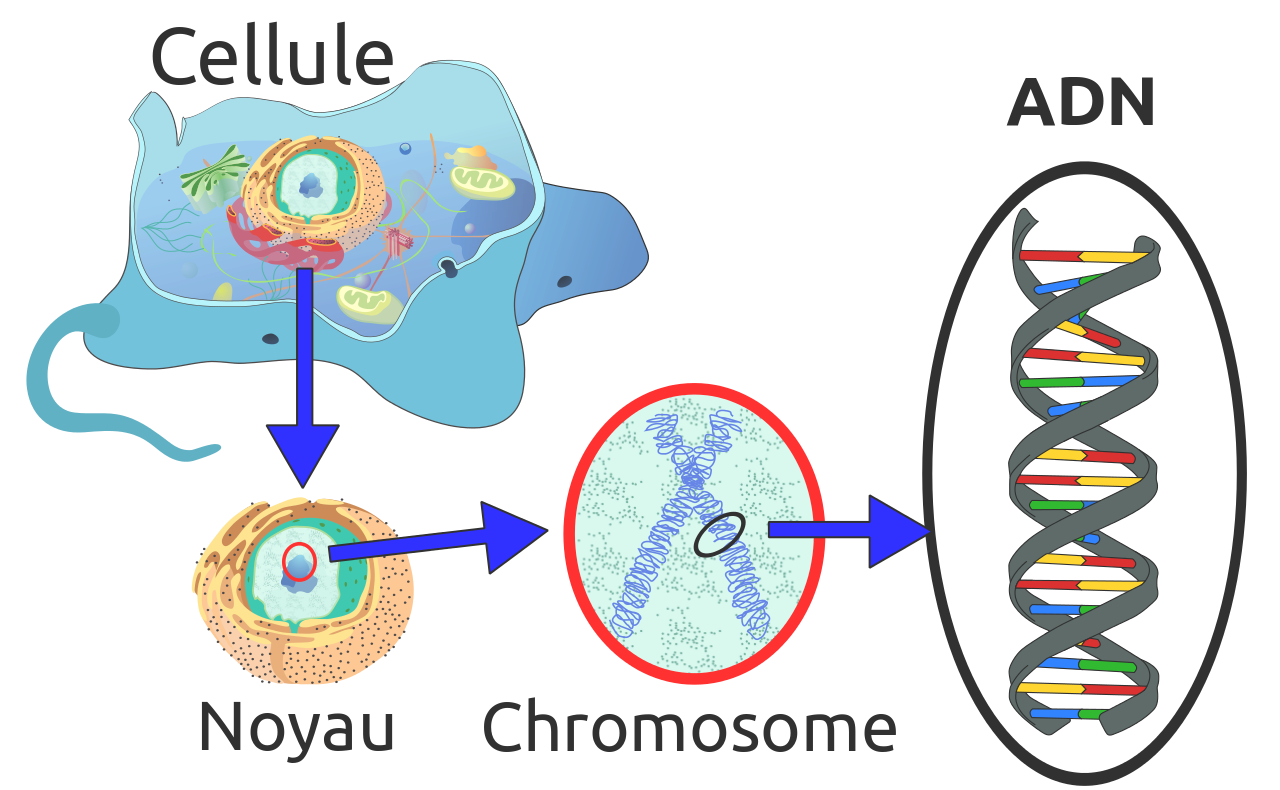
\includegraphics[width=6in]{FiguresTables/Eukaryote_DNA} 

}

\caption{Localisation de l'ADN dans une cellule eucaryote.}\label{fig:EukaryoteDNA}
\end{figure}

Le patrimoine génétique (génome) d'un individu est l'ensemble de
l'information génétique présente sous forme de chromosomes dans le noyau
des cellules eucaryotes (Figure \ref{fig:EukaryoteDNA}). L'Homme dispose
de 22 paires de chromosomes, appelés autosomes, et d'une paire de
chromosomes sexuels ou gonosomes (notés XX chez la femme, et XY chez
l'homme). Ces chromosomes constituent la forme condensée de deux
molécules, appelées brins, d'Acide DésoxyriboNucléique (ADN), et
composées de la répétition de quatre nucléotides (ou bases
nucléotidiques)~: A, C, G et T, respectivement pour adénosine, cytosine,
guanine et thymine. La position de l'une de ces bases, donnée en paire
de base (pb), est appelée locus (loci, au pluriel). Il est à noter qu'un
locus peut également désigner une région de plusieurs dizaines de paires
de bases, voire d'un gène entier. Ces quatre nucléotides sont la base de
l'information génétique et sont complémentaires pour une même paire~: A
est couplé à T, tandis que C est couplé à G. Cette complémentarité
permet aux deux brins d'ADN de se lier l'un à l'autre via une liaison
hydrogène et de former une structure en double-hélice. L'association de
cette double-hélice avec des complexes protéiques, tels que les
histones, permet à l'ADN d'être présent dans deux états de condensation
différents~: l'euchromatine, un état décondensé, et l'hétérochromatine,
un état condensé où les histones sont très rapprochées les unes des
autres. Ces deux états de condensation de la molécule d'ADN auront un
effet sur les mécanismes de transcription de l'ADN. La transcription est
un mécanisme de lecture de l'ADN et d'écriture d'une partie de
l'information génétique se trouvant au niveau d'un gène sous une forme
dérivée~: l'Acide RiboNucléique (ARN). Les gènes sont le résultat de
l'arrangement en séquence des 3,5 milliards de paires de bases du génome
humain (Ensembl version 89, mai 2017). Cependant, l'ensemble de l'ADN
n'est pas codant. Chez l'Homme, il existe environ 20 000 gènes codant
pour des protéines, répartis de façon discontinue sur l'ensemble du
génome (Ensembl version 89, mai 2017).



\begin{figure}[!htb]

{\centering 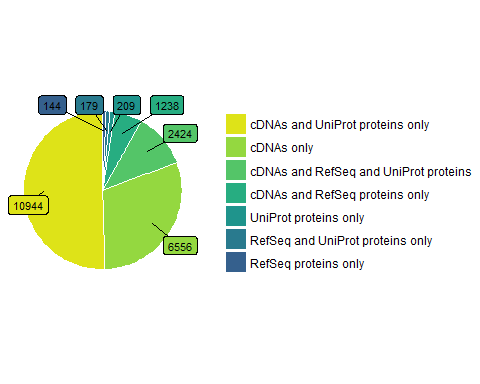
\includegraphics[width=6in,height=4in]{ArticleThesis_MickaelCanouil_files/figure-latex/ensembl-1} 

}

\caption{Diagramme des gènes répertoriés sur la base Ensembl.}\label{fig:ensembl}
\end{figure}

D'une cellule à une autre dans un même organisme, le génome est le même.
Cependant, il existe des disparités entre le génome de deux individus
d'une même espèce, et d'autant plus entre deux espèces. Ainsi, deux
individus d'une même espèce vont partager pour plusieurs loci les mêmes
allèles, mais pourront présenter des variations appelées polymorphismes.
Pour un même locus, le génotype donne l'allèle présent sur chacun des
deux chromosomes d'une même paire, et s'écrit sous la forme d'un couple
d'allèles~: AA, AB, ou BB, où A et B désignent les bases nucléotidiques
(c.-à-d. A, C, G ou T).

Au sein d'une population, la variabilité génétique est engendrée
principalement par l'intermédiaire de deux phénomènes~: la mutation ou
la recombinaison. La mutation est un mécanisme introduisant un
polymorphisme, c'est-à-dire par l'introduction d'une nouvelle version
d'un allèle au sein de la séquence, soit par l'ajout, la suppression ou
l'insertion d'un ou plusieurs nucléotides, provoquant ainsi des
changements dans la séquence d'ADN. Ces changements peuvent être classés
en différentes catégories selon leur conséquence sur la synthèse de la
protéine. Ainsi, une mutation est dite ``silencieuse'' ou ``synonyme'',
lorsque l'acide aminé n'est pas changé.



\begin{figure}[!htb]

{\centering 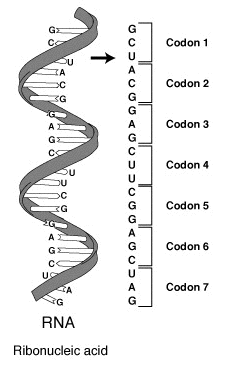
\includegraphics[width=2.3in,height=4in]{FiguresTables/RNA-codon} 

}

\caption{Brin d'ARN et codons.}\label{fig:RNAcodon}
\end{figure}

Un acide aminé est le résultat de la traduction, depuis un ARN messager,
d'une séquence de trois bases nucléotidiques nommée ``codon'' (Figure
\ref{fig:RNAcodon}). Il existe 64 codons (\(4^3\) combinaisons de
bases), correspondant à 22 acides aminés uniques, ce qui permet à
plusieurs codons d'être traduits en un même acide aminé. Quand la
mutation engendre l'apparition d'un codon stop, arrêtant par le fait
même la synthèse de la protéine avant la fin de la séquence d'ARN, elle
est alors appelée ``non-sens''.

La recombinaison est un mécanisme se produisant lors de la méiose,
c'est-à-dire lors du processus de formation des gamètes, où les
chromosomes homologues (c.-à-d. les chromosomes d'une même paire) se
chevauchent, et peuvent alors échanger une partie de l'ADN les
constituant. La recombinaison n'affecte pas l'ensemble du chromosome de
façon homogène. En effet, les événements de recombinaison sont plus
fréquents avec l'éloignement du centromère, c'est-à-dire à la position
de jointure des chromosomes d'une même paire. On parle de déséquilibre
de liaison lorsque la probabilité d'observer un allèle à un locus A
n'est pas indépendante de celle d'observer un allèle à un locus B,
autrement dit, lorsque la probabilité d'observer un certain couple
d'allèle n'est pas égale au produit au produit des probabilités
d'observé chaque allèle individuellement.

Pour la suite, nous nous intéresserons principalement aux variants
génétiques polymorphiques au niveau d'une seule base nucléotidique, les
SNPs (``Single Nucleotide Polymorphisms''), et omettrons les
insertions/délétions (INDEL), ou encore les variations du nombre de
copies ou CNVs (``Copy Number Variations'').

\subsection{Transcriptome}\label{transcriptome}




\begin{figure}[!htb]

{\centering 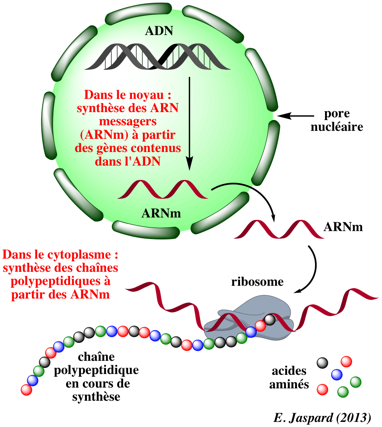
\includegraphics[width=4in]{FiguresTables/2LocalGlobale} 

}

\caption{Schéma simplifié de la synthèse des protéines chez
les eucaryotes.}\label{fig:LocalGlobale}
\end{figure}

La transcriptomique étudie les ARN formés lors de la transcription d'un
gène dans le noyau. La transcription est une étape indispensable pour la
synthèse de protéines permettant de faire transiter l'information
contenue dans l'ADN nucléaire vers le cytoplasme sous la forme d'ARN, où
se trouve le matériel nécessaire à la traduction en protéine (c.-à-d.
les ribosomes et les acides aminés) (Figure \ref{fig:LocalGlobale}). La
transcription de l'ADN en ARN est réalisée par l'enzyme ARN polymérase.
Il existe plusieurs classes d'ARN, dont la plus abondante est la classe
des ARN messagers (mRNA).



\begin{figure}[!htb]

{\centering 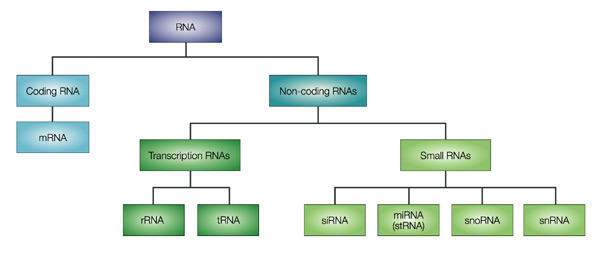
\includegraphics[width=6in]{FiguresTables/RNAtype} 

}

\caption{Classification des différents types d'ARN.}\label{fig:RNAtype}
\end{figure}

À cette classe s'ajoutent les ARN de transfert (tRNA), qui apportent les
acides aminés nécessaires à la traduction des mRNA en protéines, et les
ARN ribosomaux (rRNA), qui constituent les complexes protéiques que sont
les ribosomes, ainsi que des ARN mesurant moins de 200 nucléotides, soit
les petits ARN (``small RNA''), les miRNA (``microRNA''), les snoRNA
(``small nucleolar RNA''), les siRNA (``small interfering RNA''), les
piRNA (``piwi interfering RNA''), etc. (Figure \ref{fig:RNAtype}). Ces
derniers participent à divers mécanismes métaboliques, notamment la
régulation de l'expression des gènes
\citep{ambros_functions_2004, bartel_micrornas:_2004}.

L'expression des gènes est mesurée directement par les mRNA, qui
représentent les ARN codant pour les protéines. Il est à noter que le
nombre de protéines pouvant être synthétisé est supérieur au nombre de
gènes. En effet, un gène se compose de plusieurs exons (parties
codantes) et d'introns (parties non-codantes), et lors de la
transcription, l'épissage du gène permet la création d'une molécule mRNA
ne comportant que les parties codantes. Cette phase d'épissage peut être
``alternative'', c'est-à-dire, que pourront être conservées, lors de la
synthèse de mRNA, différentes combinaisons d'exons aboutissant à la
synthèse de plusieurs mRNA ou transcrits, qui seront alors exportés en
dehors du noyau pour être ensuite synthétisés en protéines dans le
cytoplasme de la cellule. Ainsi, un gène peut produire plusieurs
protéines différentes selon les besoins et la fonction de la cellule et
du tissu. Le transcriptome est défini comme l'ensemble des ARN présents
à un instant donné dans un tissu ou type cellulaire spécifique, et
nécessaires à la synthèse protéique et à sa régulation en partie via les
petits ARN.

\subsection{Épigénome et Méthylome}\label{epigenome-et-methylome}

Les mécanismes de régulation de l'expression des gènes sont nombreux.
L'un de ces mécanismes passe par des marques épigénétiques modifiant la
structure et la conformation de l'ADN, rendant de ce fait plus simple ou
plus difficile selon les cas, la fixation des facteurs de transcription,
et plus généralement de la machinerie cellulaire sur l'ADN. Il existe
principalement deux types de modifications épigénétiques~: la
méthylation de l'ADN et les modifications d'histones. L'ensemble de ces
modifications constitue l'épigénome d'un individu. Le méthylome
constitue un sous-ensemble de l'épigénome regroupant uniquement les
marques de méthylation. Nous nous concentrerons sur le méthylome
impliqué principalement dans la régulation des gènes, la maintenance et
la formation de la chromatine, constituant de ce fait un élément
important de la régulation du transcriptome.



\begin{figure}[!htb]

{\centering 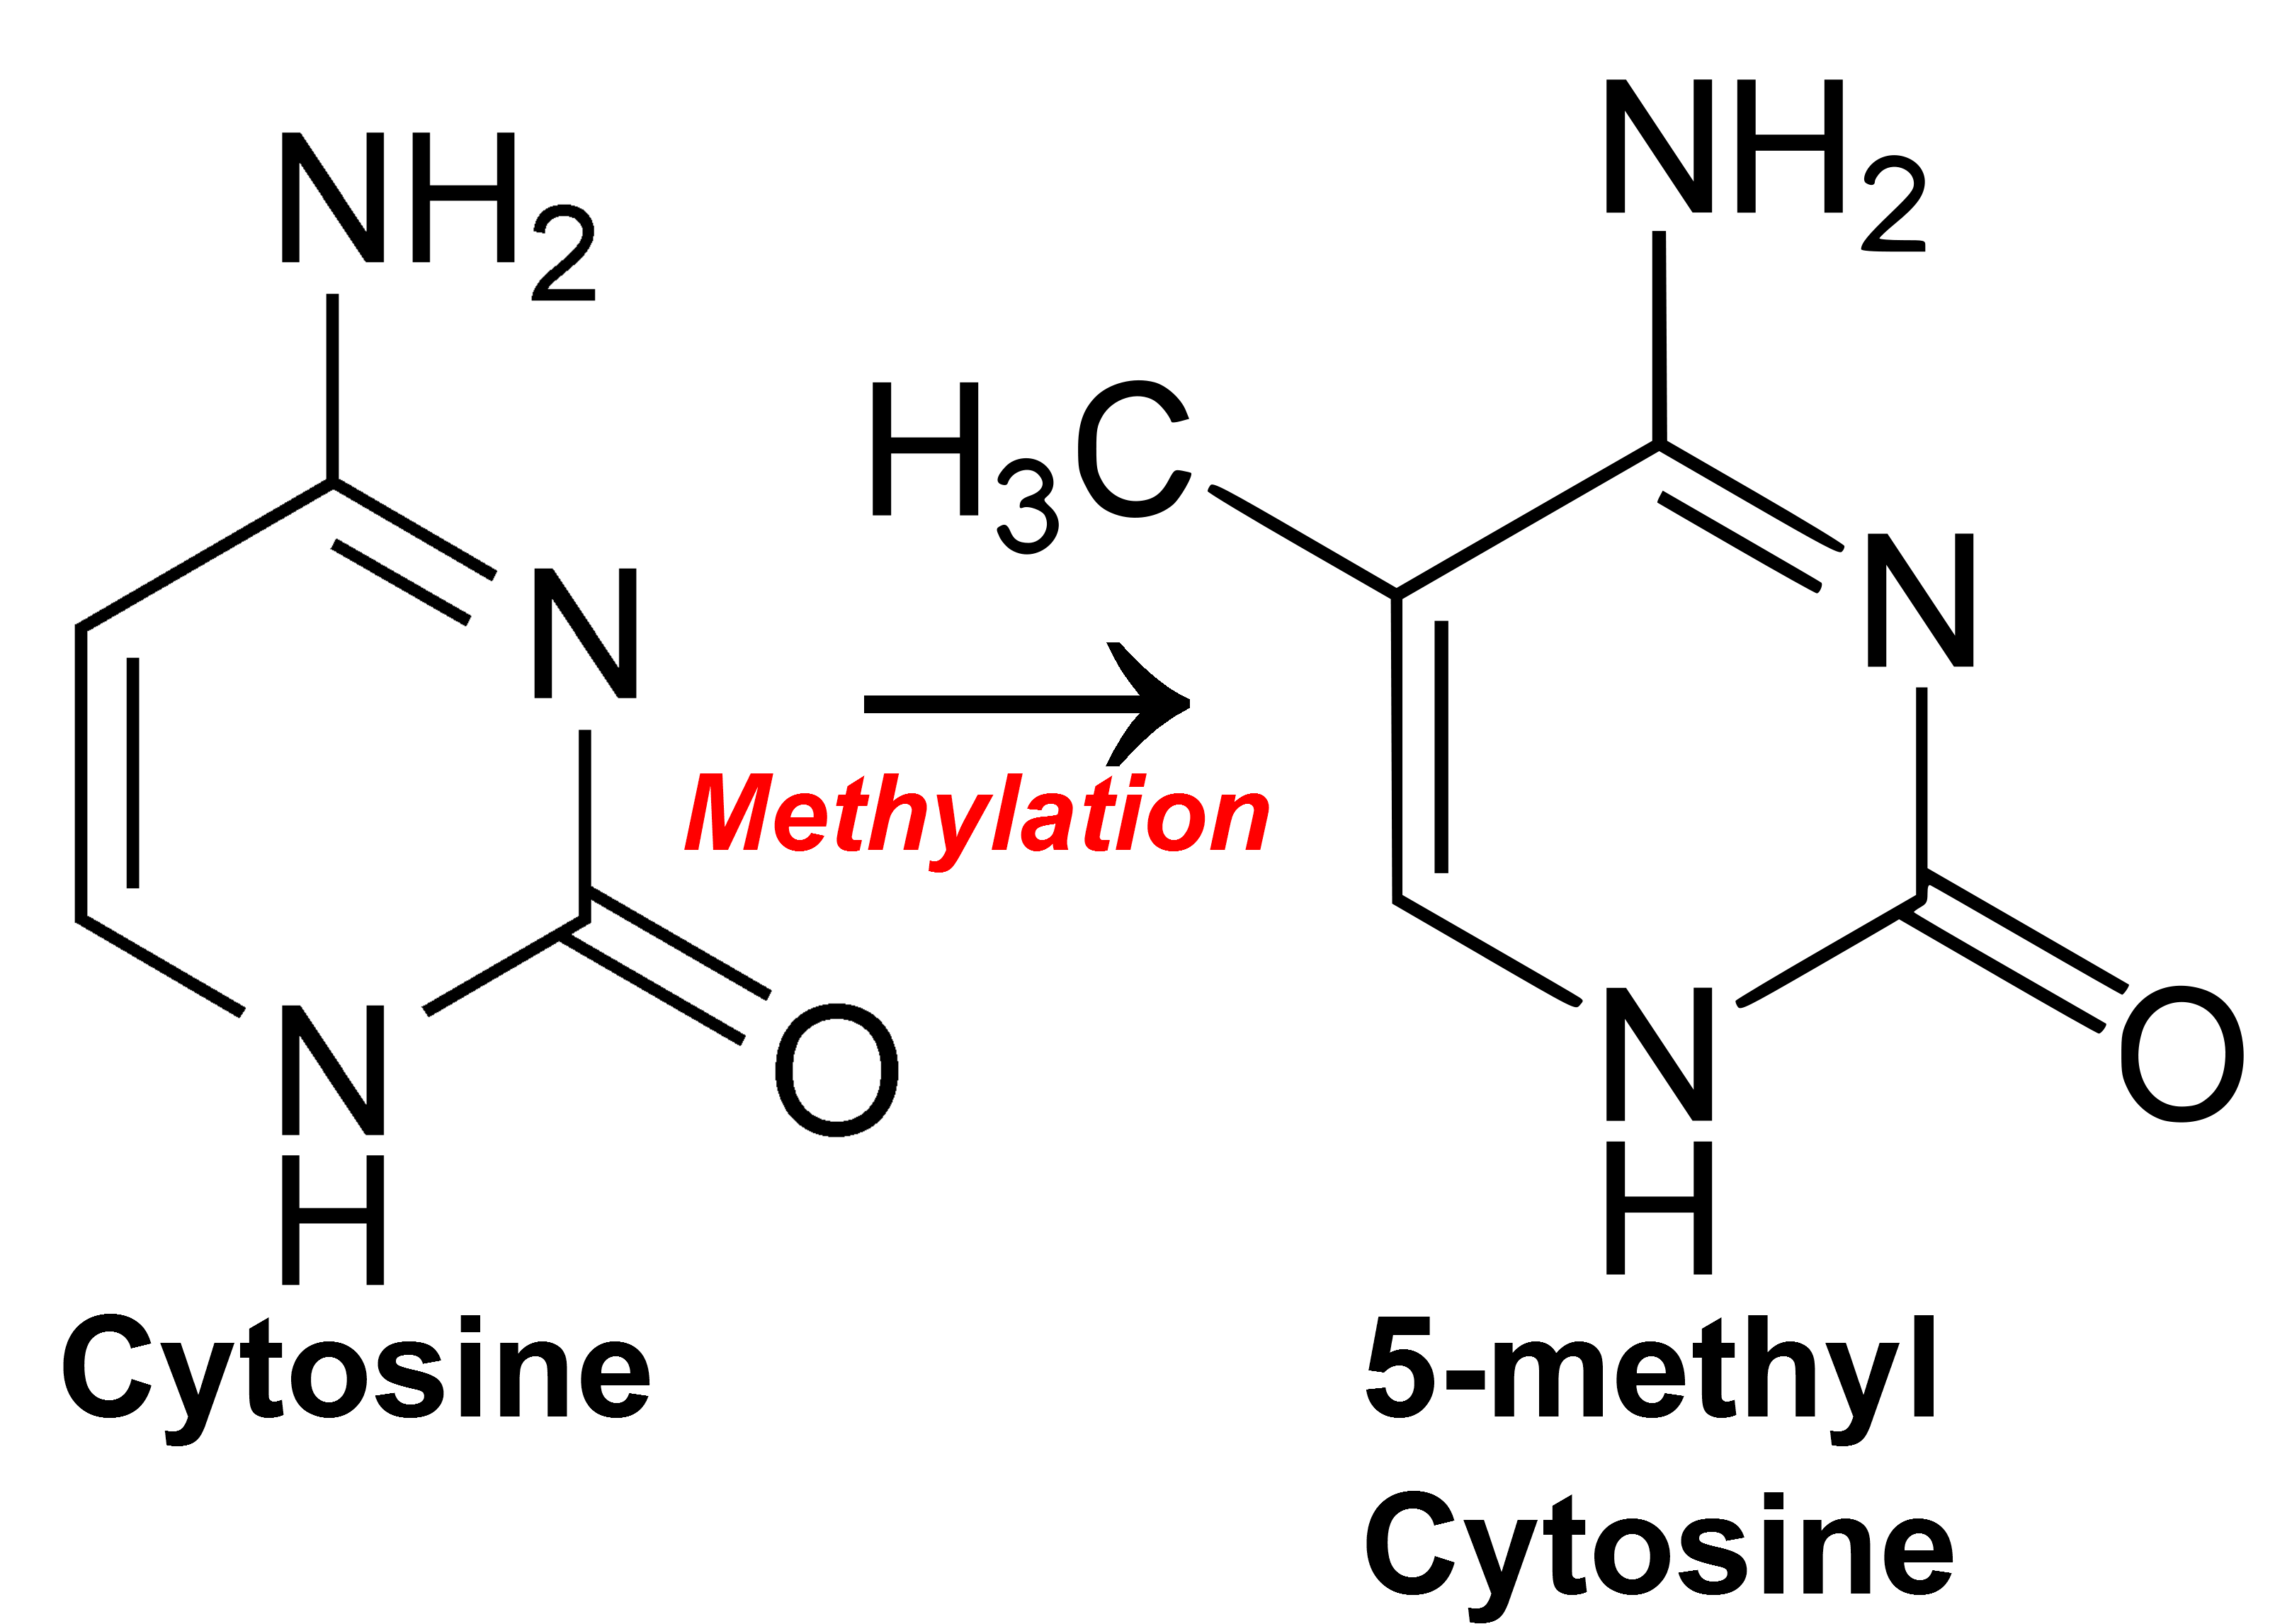
\includegraphics[width=3in]{FiguresTables/cytosine} 

}

\caption{Formule structurelle de la méthylation de la cytosine.}\label{fig:cytosine}
\end{figure}

La méthylation de l'ADN est l'ajout d'un groupement méthyl via une
enzyme de la famille des ADN méthyltransférases (\emph{DNMT}). Cette
enzyme va catalyser l'ajout d'un groupement méthyl sur le carbone en
position 5 d'une cytosine (5mC), cytosine généralement suivie (5' vers
3') d'une guanine, formant ainsi un groupement CpG
(cytosine-phosphate-guanine) (Figure \ref{fig:cytosine}). Ces
groupements, ou sites CpG, ne sont pas les seuls groupements de
dinucléotides pouvant faire l'objet d'une méthylation CpHpG (H = A, T,
ou C) \citep{lister_human_2009}. Cependant, ces marques ne sont pas les
plus fréquentes chez les organismes eucaryotes \citep{bird_dna_1980}.

Les sites CpG représentent une faible fraction du génome
(\(\simeq 1 \%\)) et sont distribués de façon hétérogène sur l'ensemble
du génome en raison d'une déamination spontanée, au cours du temps, des
5mC en thymine \citep{bird_dna_1980, cooper_cytosine_1989}.




\begin{figure}[!htb]

{\centering 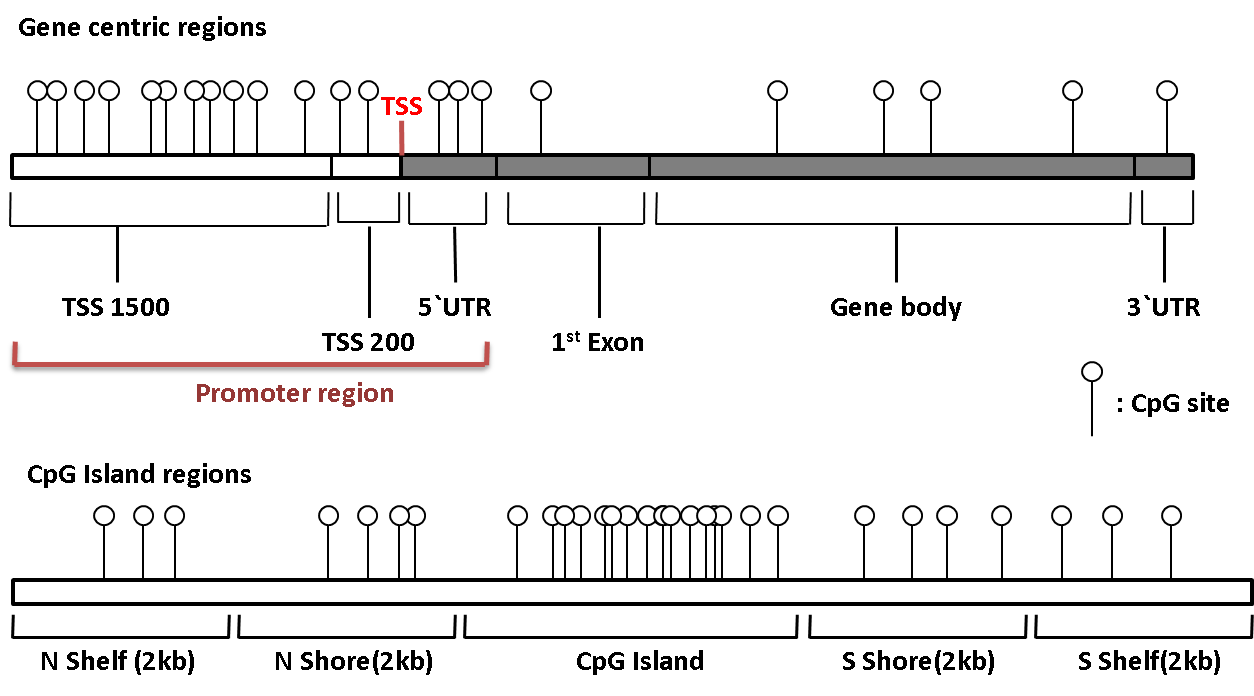
\includegraphics[width=6in]{FiguresTables/CpG} 

}

\caption{Schéma représentant la localisation des sites CpG sur le
génome.}\label{fig:CpG}
\end{figure}

Les sites CpG peuvent être regroupés en îlots, appelés îlots CpG
\citep{deaton_cpg_2011} (Figure \ref{fig:CpG}). Ces îlots CpG sont des
régions enrichies en dinucléotide guanine-cytosine (GC) et sont
généralement non-méthylés. Un îlot CpG est défini comme une séquence
d'une longueur de 200 à 1 000 paires de bases comportant plus de 50~\%
de GC et un ratio \(\frac{CpG_{observé}}{CpG_{attendu}}>=60\)~\%
\citep{antequera_structure_2003, gardiner-garden_cpg_1987}. Ces îlots
CpG sont localisés dans les régions promotrices et exoniques pour 40 à
60~\% d'entre eux \citep{larsen_cpg_1992, saxonov_genome-wide_2006},
traduisant l'importance du processus de méthylation dans la régulation
de l'expression des gènes. Les sites et îlots CpG sont principalement
déméthylés lorsqu'ils sont situés dans des régions promotrices (p.~ex.
site d'initiation de la transcription, en amont d'un gène) et des exons,
et sont méthylés lorsqu'ils sont localisés dans le corps des gènes
\citep{ball_targeted_2009, hellman_gene_2007, jones_dna_1999}. En effet,
une hypométhylation observée au niveau des régions promotrices de la
transcription est généralement inversement corrélée avec l'expression
des gènes \citep{schultz_human_2015, wagner_relationship_2014}, mais pas
de façon systématique \citep{moarii_changes_2015}, rendant complexe
l'étude de l'épigénome conjointement avec le transcriptome. À cela
s'ajoute l'impact potentiel des mutations survenant au niveau de la
cytosine d'un site CpG. Ces polymorphismes sont appelés CpG-SNPs et
permettent de mettre en évidence des mécanismes d'interaction entre
génome et épigénome \citep{dayeh_identification_2013, zhi_snps_2013}.

\subsection{Phénotype}\label{phenotype}

Le phénotype correspond à l'ensemble des caractères ou traits physiques
observables chez un individu (p.~ex. la taille, la couleur des yeux, le
statut diabétique, etc.). Le phénotype est le résultat à la fois du
génotype et des facteurs environnementaux, comme le mode de vie, le
régime alimentaire ou l'activité physique par exemple. Un biomarqueur
est une marque phénotypique particulière qui est la mesure d'un composé
(p.~ex. protéine, métabolite, etc.) présent dans le corps d'un individu
et servant, en médecine, à des fins diagnostiques d'une pathologie.

\section{Le diabète de type 2}\label{le-diabete-de-type-2}

\subsection{Définition et chiffres du
diabète}\label{definition-et-chiffres-du-diabete}

Le diabète est défini par une hyperglycémie. Dès 1999, l'organisation
Mondiale de la Santé (OMS)
\citep{world_health_organization_definition_1999} préconise deux mesures
de glycémie pour diagnostiquer le diabète~: la glycémie à jeun et la
glycémie mesurée deux heures après un test de tolérance au glucose par
voie orale (OGTT). Dans la pratique, le diagnostic du diabète
s'effectue, dans certains cas, via la mesure d'hémoglobine glyquée
(HbA1c).\\
C'est notamment le cas aux États-Unis, où la mesure d'HbA1c fait partie
des critères de définition proposés par l'Association Américaine pour le
Diabète (ADA). L'HbA1c est utilisée ici pour sa propriété à refléter
l'évolution de la glycémie sur les trois derniers mois, ce qui
correspond à la durée de vie moyenne d'un d'érythrocyte.

\begin{table}

\caption{\label{tab:t2ddefinitionOMS}Critères glycémiques de l'organisation mondiale de la santé (OMS), définissant les statuts insulinorésistant et diabétique. (OGTT : test de tolérance au glucose par voie orale).}
\centering
\begin{tabular}[t]{lll}
\toprule
 & Glycémie à jeun & Glycémie 2h après OGTT\\
\midrule
Normoglycémique & < 6,1 mmol/L & < 7,7 mmol/L\\
Intolérant au glucose & 6,1 - 6,9 mmol/L & 7,7 - 11 mmol/L\\
Diabétique & > 7 mmol/L & > 11,1 mmol/L\\
\bottomrule
\end{tabular}
\end{table}

\begin{table}

\caption{\label{tab:t2ddefinitionADA}Critères glycémiques de l'association américaine pour le diabète (ADA), définissant les statuts insulinorésistant et diabétique.}
\centering
\begin{tabular}[t]{lll}
\toprule
 & Glycémie à jeun & HbA1c\\
\midrule
Normoglycémique & < 5,6 mmol/L & > 5,7 \%\\
Intolérant au glucose & 5,6 - 6,9 mmol/L & 5,7 - 6,4 \%\\
Diabétique & > 7 mmol/L & > 6,5 \%\\
\bottomrule
\end{tabular}
\end{table}

Même si l'ADA et l'OMS s'accordent pour définir le diabète à partir
d'une glycémie à jeun supérieure à 7,0 mmol/L, les critères pour définir
une glycémie normale diffèrent entre les deux organisations, avec un
seuil de glycémie inférieure à 5,6 mmol/L pour l'ADA et 6,1 mmol/L pour
l'OMS (Tableau \ref{tab:t2ddefinitionOMS} et
\ref{tab:t2ddefinitionADA}). Cette phase, ainsi définie pour une
glycémie entre 5,6 ou 6,1 mmol/L et 7 mmol/L, peut être transitoire vers
un diabète, et est parfois appelée ``prédiabète''. Les patients
diagnostiqués comme intolérants au glucose font l'objet d'une prise en
charge préventive consistant principalement en une modification du
comportement alimentaire et plus généralement des habitudes de vie.

L'hyperglycémie chronique peut, lorsqu'elle n'est pas traitée, provoquer
des complications au niveau cardiovasculaire, rénale, oculaire, et dans
certains cas, conduire à une amputation d'un ou des membres inférieurs.
Selon le dernier rapport de l'OMS, plus de 400 millions de personnes en
2014 vivaient avec le diabète, contre seulement 108 millions en 1980
selon les estimations mondiales \citep{roglic_global_2016}. Depuis 1980,
la prévalence du diabète est passée de 4,7 à 8,5~\% chez la population
adulte dans le monde.\\
En France, selon les derniers rapports de l'Institut de Veille Sanitaire
(InVS) \citep{mandereau-bruno_prevalence_2014, ricci_diabete_2010}, la
prévalence du diabète traité est passée de 4,6~\% en 2012 à 5~\% en
2015. En 2006-2007, la prévalence de l'intolérance au glucose
représentait 5,6~\%, ce qui en fait un véritable enjeu de santé
publique.

Il existe 4 formes de diabète, le diabète de type 1, le diabète de type
2, le diabète gestationnel et les diabètes monogéniques.\\
Le diabète de type 1 est le diabète dit insulinodépendant et nécessite
des injections régulières d'insuline. Ce diabète se développe
généralement chez un individu jeune qui perd rapidement sa capacité à
réguler sa glycémie, suite à une réaction auto-immune contre les
cellules \(\beta\) du pancréas (cellules sécrétrices de l'insuline).\\
Le diabète de type 2 est parfois appelé diabète de l'adulte ou diabète
non-insulinodépendant, par opposition au diabète de type 1. Il se
caractérise principalement par un défaut du métabolisme de l'insuline
d'un ou plusieurs organes. Le diabète de type 2 représente plus de 90~\%
des diabètes dans le monde \citep{lyssenko_genetic_2013}. Parce que les
symptômes du diabète de type 2 sont moins marqués que ceux du diabète de
type 1, le diabète de type 2 est souvent diagnostiqué tardivement, et
notamment suite aux complications résultantes de celui-ci. Le diabète
existe également sous une troisième forme, dit gestationnel. Ce diabète
survient chez la femme durant la grossesse, aux environs de la 24ème
semaine d'aménorrhée, et présente un facteur de risque accru du
développement ultérieur d'un diabète de type 2, à la fois chez la mère
et chez l'enfant \citep{case_preventing_2006, roglic_global_2016}.

\subsection{Physiopathologie du diabète de type
2}\label{physiopathologie-du-diabete-de-type-2}





\begin{figure}[!htb]

{\centering 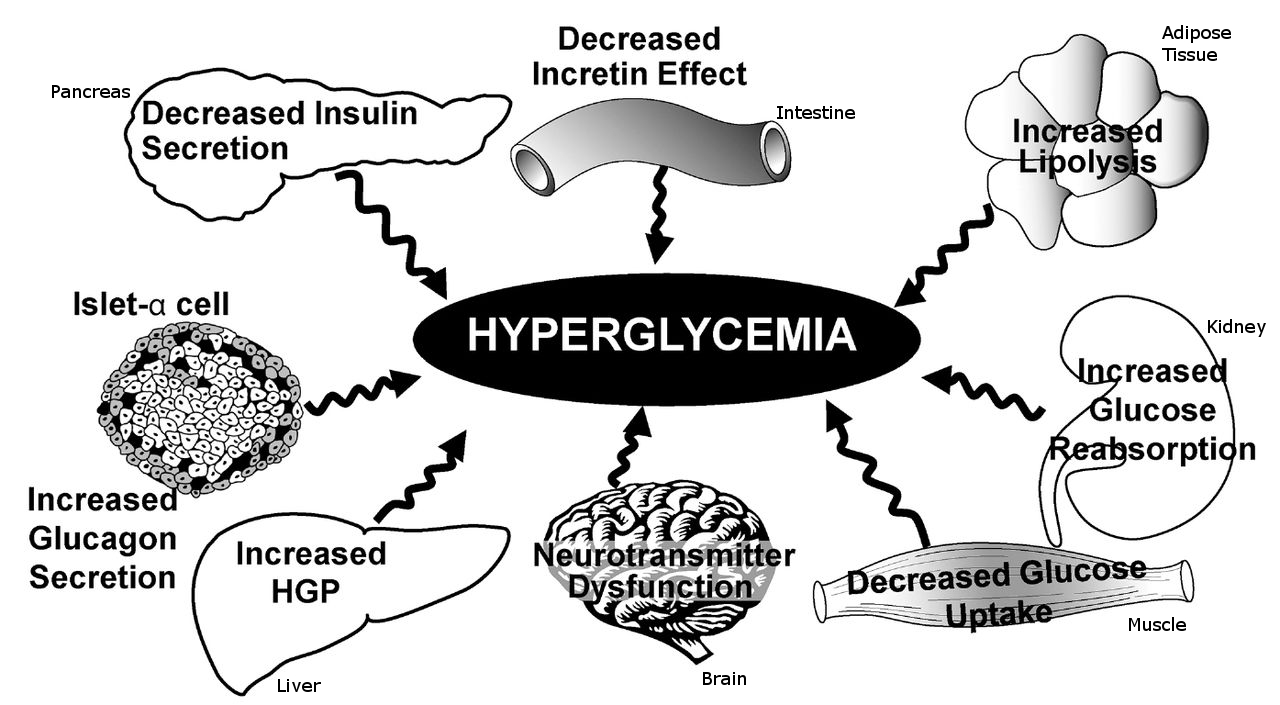
\includegraphics[width=6in]{FiguresTables/hyperglycemia_t2d} 

}

\caption{Tissus et organes impliqués dans l'hyperglycémie et
le diabète de type 2 (HGP~: ``hepatic glucose production'', production
hépatique de glucose).}\label{fig:hyperglycemia}
\end{figure}

Le diabète de type 2 serait la conséquence d'une production insuffisante
d'insuline en réponse à une demande accrue de l'organisme provenant
d'une résistance à l'insuline
\citep{world_health_organization_definition_1999, world_health_organization_definition_2006}.
Le diabète de type 2 est une pathologie complexe dont l'origine
génétique est multiple et passe notamment par des interactions avec
l'environnement. De nombreux traits ont été identifiés comme facteurs de
risque, tels le sexe, l'âge ou encore l'Indice de Masse Corporel (IMC),
mais aussi l'ethnicité (p.~ex., population des indiens Pima
\citep{diamond_double_2003, knowler_determinants_1993}) et le manque
d'activité physique font également partie de ces facteurs de risques
\citep{lyssenko_clinical_2008, mykkanen_cardiovascular_1993, noble_risk_2011}.\\
L'hyperglycémie, dans le cadre du diabète de type 2, implique trois
mécanismes principaux~: i) une augmentation de la sécrétion de glucose
par le foie (néoglucogenèse)~; ii) une diminution de l'entrée et donc du
métabolisme du glucose dans les organes périphériques, comme le muscle
(insulinorésistance)~; iii) une altération de la sécrétion d'insuline
par le pancréas ou une altération de l'insuline elle-même (Figure
\ref{fig:hyperglycemia}).

L'insulinémie et la glycémie à jeun permettent de mesurer
l'insulinorésistance sur la base des indices HOMA (``HOmeostasis Model
Assessment'') \citep{matthews_homeostasis_1985}. Trois indices HOMA ont
été proposés, avec \(I\), l'insulinémie à jeun (en mU/L) et avec \(G\),
la glycémie à jeun (en mmol/L)~:

\begin{itemize}
\item
  l'HOMA-IR reflétant l'insulinorésistance, dont la valeur normale est
  établie à 1, et qui augmente avec la gravité de l'insulinorésistance
  (\(\textrm{HOMA-IR}=\frac{(I\times G)}{22,5}\))~;
\item
  l'HOMA-B augmentant avec l'altération de la fonction des cellules
  \(\beta\), dont la valeur normale est fixée à 100~\%
  (\(\textrm{HOMA-B}=\frac{(20\times I)}{(G-3,5)}\))~;
\item
  l'HOMA-S étant l'inverse de l'HOMA-IR et représentant la sensibilité à
  l'insuline (\(\textrm{HOMA-S}=\frac{1}{\textrm{HOMA-IR}}\times 100\)).
\end{itemize}

Depuis la formulation de ces indices, \citet{levy_correct_1998} ont
proposé un nouveau modèle HOMA2, permettant la prise en compte de la
variabilité de la tolérance au glucose du foie et des tissus
périphériques, de la contribution à l'homéostasie de la proinsuline
circulante, ainsi qu'une meilleure définition de la courbe de sécrétion
d'insuline en réponse au glucose, notamment pour des concentrations en
glucose supérieures à 10 mmol/L. Les indices basés sur le modèle HOMA2
sont exprimés en pourcentage, contrairement aux indices HOMA.

L'insulinorésistance correspond à la perte de sensibilité des récepteurs
cibles de l'insuline, ne permettant plus à l'insuline de se fixer et
bloquant ainsi l'entrée du glucose dans la cellule. Cette
insulinorésistance engendre une sécrétion plus importante d'insuline par
les cellules \(\beta\) pour compenser ce manque d'efficacité (partielle
ou totale), entraînant à plus ou moins long terme la défaillance de ces
cellules, et dans le même temps induisant une hyperglycémie, signe
précurseur d'un potentiel diabète. L'insulinorésistance des tissus se
traduit, en plus de l'augmentation de la néoglucogenèse (dans le foie)
et la diminution de l'entrée du glucose dans les cellules, par une
augmentation de la libération d'acide-gras dans le tissu adipeux
(lipolyse). Cette augmentation de la lipolyse tend à aggraver les mêmes
phénomènes ayant initialement induit celle-ci, à savoir l'aggravation de
l'insulinorésistance, l'augmentation de la néoglucogenèse hépatique et
la diminution de l'action et de la sécrétion de l'insuline.

\subsection{La maladie du foie non
alcoolique}\label{la-maladie-du-foie-non-alcoolique}

Les complications du diabète, et plus généralement les pathologies
associées, sont variées et peuvent toucher tous les tissus. En
conséquence, l'étude de la physiopathologie du diabète de type 2
nécessite de comprendre les mécanismes biologiques, génétiques et
épigénétiques, impliqués dans l'ensemble des tissus connus comme ayant
un rôle dans l'hyperglycémie et l'insulinorésistance (Figure
\ref{fig:hyperglycemia}).

Ainsi, les risques de maladies de peau, rétinopathie, neuropathie,
néphropathie, ainsi que les pathologies cardiovasculaires (p.~ex.
accident cardiovasculaire, accident vasculaire cérébral et hypertension)
sont accrus chez les individus diabétiques. À ces pathologies s'ajoutent
des pathologies spécifiques du foie, rangées principalement sous
l'appellation NAFLD (``Non-Alcoholic Fatty Liver Disease'') et NASH
(``Non-Alcoholic Steato-Hepatitis'') dans les cas les plus sévères. Ces
dernières pathologies se définissent à partir de l'évaluation de
différents critères, au moyen d'une coupe histologique d'un échantillon
de biopsie du foie~:

\begin{itemize}
\item
  Stéatose~: pourcentage d'accumulation de triglycérides, se
  caractérisant par la déformation des hépatocytes et l'apparition de
  taches blanches~;
\item
  Inflammation lobulaire~: inflammation et infiltration des lobules du
  foie, entrainant des lésions du tissu~;
\item
  Ballonnement hépatocytaire~: comptage des hépatocytes présentant un
  gonflement anormal et une transparence accrue.
\end{itemize}

Ces trois critères servent à établir un score, le ``NAFLD Activity
Score'' (NAS) (Tableau \ref{tab:nas}) \citep{kleiner_design_2005}. À
cela s'ajoute une potentielle fibrose du foie se caractérisant par la
destruction d'une partie du tissu hépatique, et pouvant aboutir à une
cirrhose, voire au développement d'un carcinome hépatique.



\begin{longtable}[]{@{}ccc@{}}
\caption{\label{tab:nas}Critères constituant le score NAS (``NAFLD Activity Score'').}\tabularnewline
\toprule
Critère & Score & Catégorie\tabularnewline
\midrule
\endfirsthead
\toprule
Critère & Score & Catégorie\tabularnewline
\midrule
\endhead
Stéatose & 0 & \textless{}5\%\tabularnewline
& 1 & 5-33\%\tabularnewline
& 2 & \textgreater{}33-66\%\tabularnewline
& 3 & \textgreater{}66\%\tabularnewline
Inflammation Lobulaire & 0 & Pas de foci\tabularnewline
& 1 & \textless{}2 foci/200x\tabularnewline
& 2 & 2-4 foci/200x\tabularnewline
& 3 & \textgreater{}4 foci/200x\tabularnewline
Ballonnement hépatocytaire & 0 & Aucune cellule\tabularnewline
& 1 & Quelques cellules\tabularnewline
& 2 & Beaucoup de cellules\tabularnewline
\bottomrule
\end{longtable}

\subsection{La génétique et l'épigénétique du diabète de type
2}\label{la-genetique-et-lepigenetique-du-diabete-de-type-2}




\begin{longtable}[]{@{}lccc@{}}
\caption{\label{tab:MODY}Gènes identifiés dans les diabètes de type MODY
(``Maturity-Onset Diabetes of the Young'').}\tabularnewline
\toprule
& Gène muté & Chromosome & Année de découverte\tabularnewline
\midrule
\endfirsthead
\toprule
& Gène muté & Chromosome & Année de découverte\tabularnewline
\midrule
\endhead
MODY 1 & HNF-4-alfa & 20 & 1991\tabularnewline
MODY 2 & Glucokinase & 7 & 1992\tabularnewline
MODY 3 & HNF-1-alfa & 12 & 1994\tabularnewline
MODY 4 & IPF-1 & 13 & 1997\tabularnewline
MODY 5 & HNF-1-beta & 17 & 1997\tabularnewline
MODY 6 & NeuroD1 & 2 & 1999\tabularnewline
\bottomrule
\end{longtable}

Le diabète de type 2 présente une composante génétique dont les premiers
éléments ont été mis en évidence dans des études portant sur des jumeaux
(monozygotes et dizygotes) \citep{kaprio_concordance_1992}, des études
d'agrégation familiale, ainsi que des études portant sur des formes
monogéniques de diabète, comme les diabètes dits ``Maturity-Onset
Diabetes of the Young'' (MODY) \citep{thanabalasingham_diagnosis_2011},
ou diabète de type adulte chez le jeune. Les diabètes de type MODY
n'impliquent qu'un seul gène (ou quelques-uns) (Tableau \ref{tab:MODY}).
Par exemple, un individu caractérisé MODY 2 présentera une mutation au
niveau du gène \emph{GCK} (Glucokinase), gène impliqué dans la
régulation de la glycémie transformant le glucose en
glucose-6-phosphate. Il a été montré qu'avoir un parent diabétique
augmente le risque de développer un diabète de l'ordre de 30 à 40~\%. Ce
risque augmente à 70~\% lorsque les deux parents sont diabétiques
\citep{kobberling_empirical_1982, meigs_parental_2000}.








\begin{figure}[!htb]

{\centering 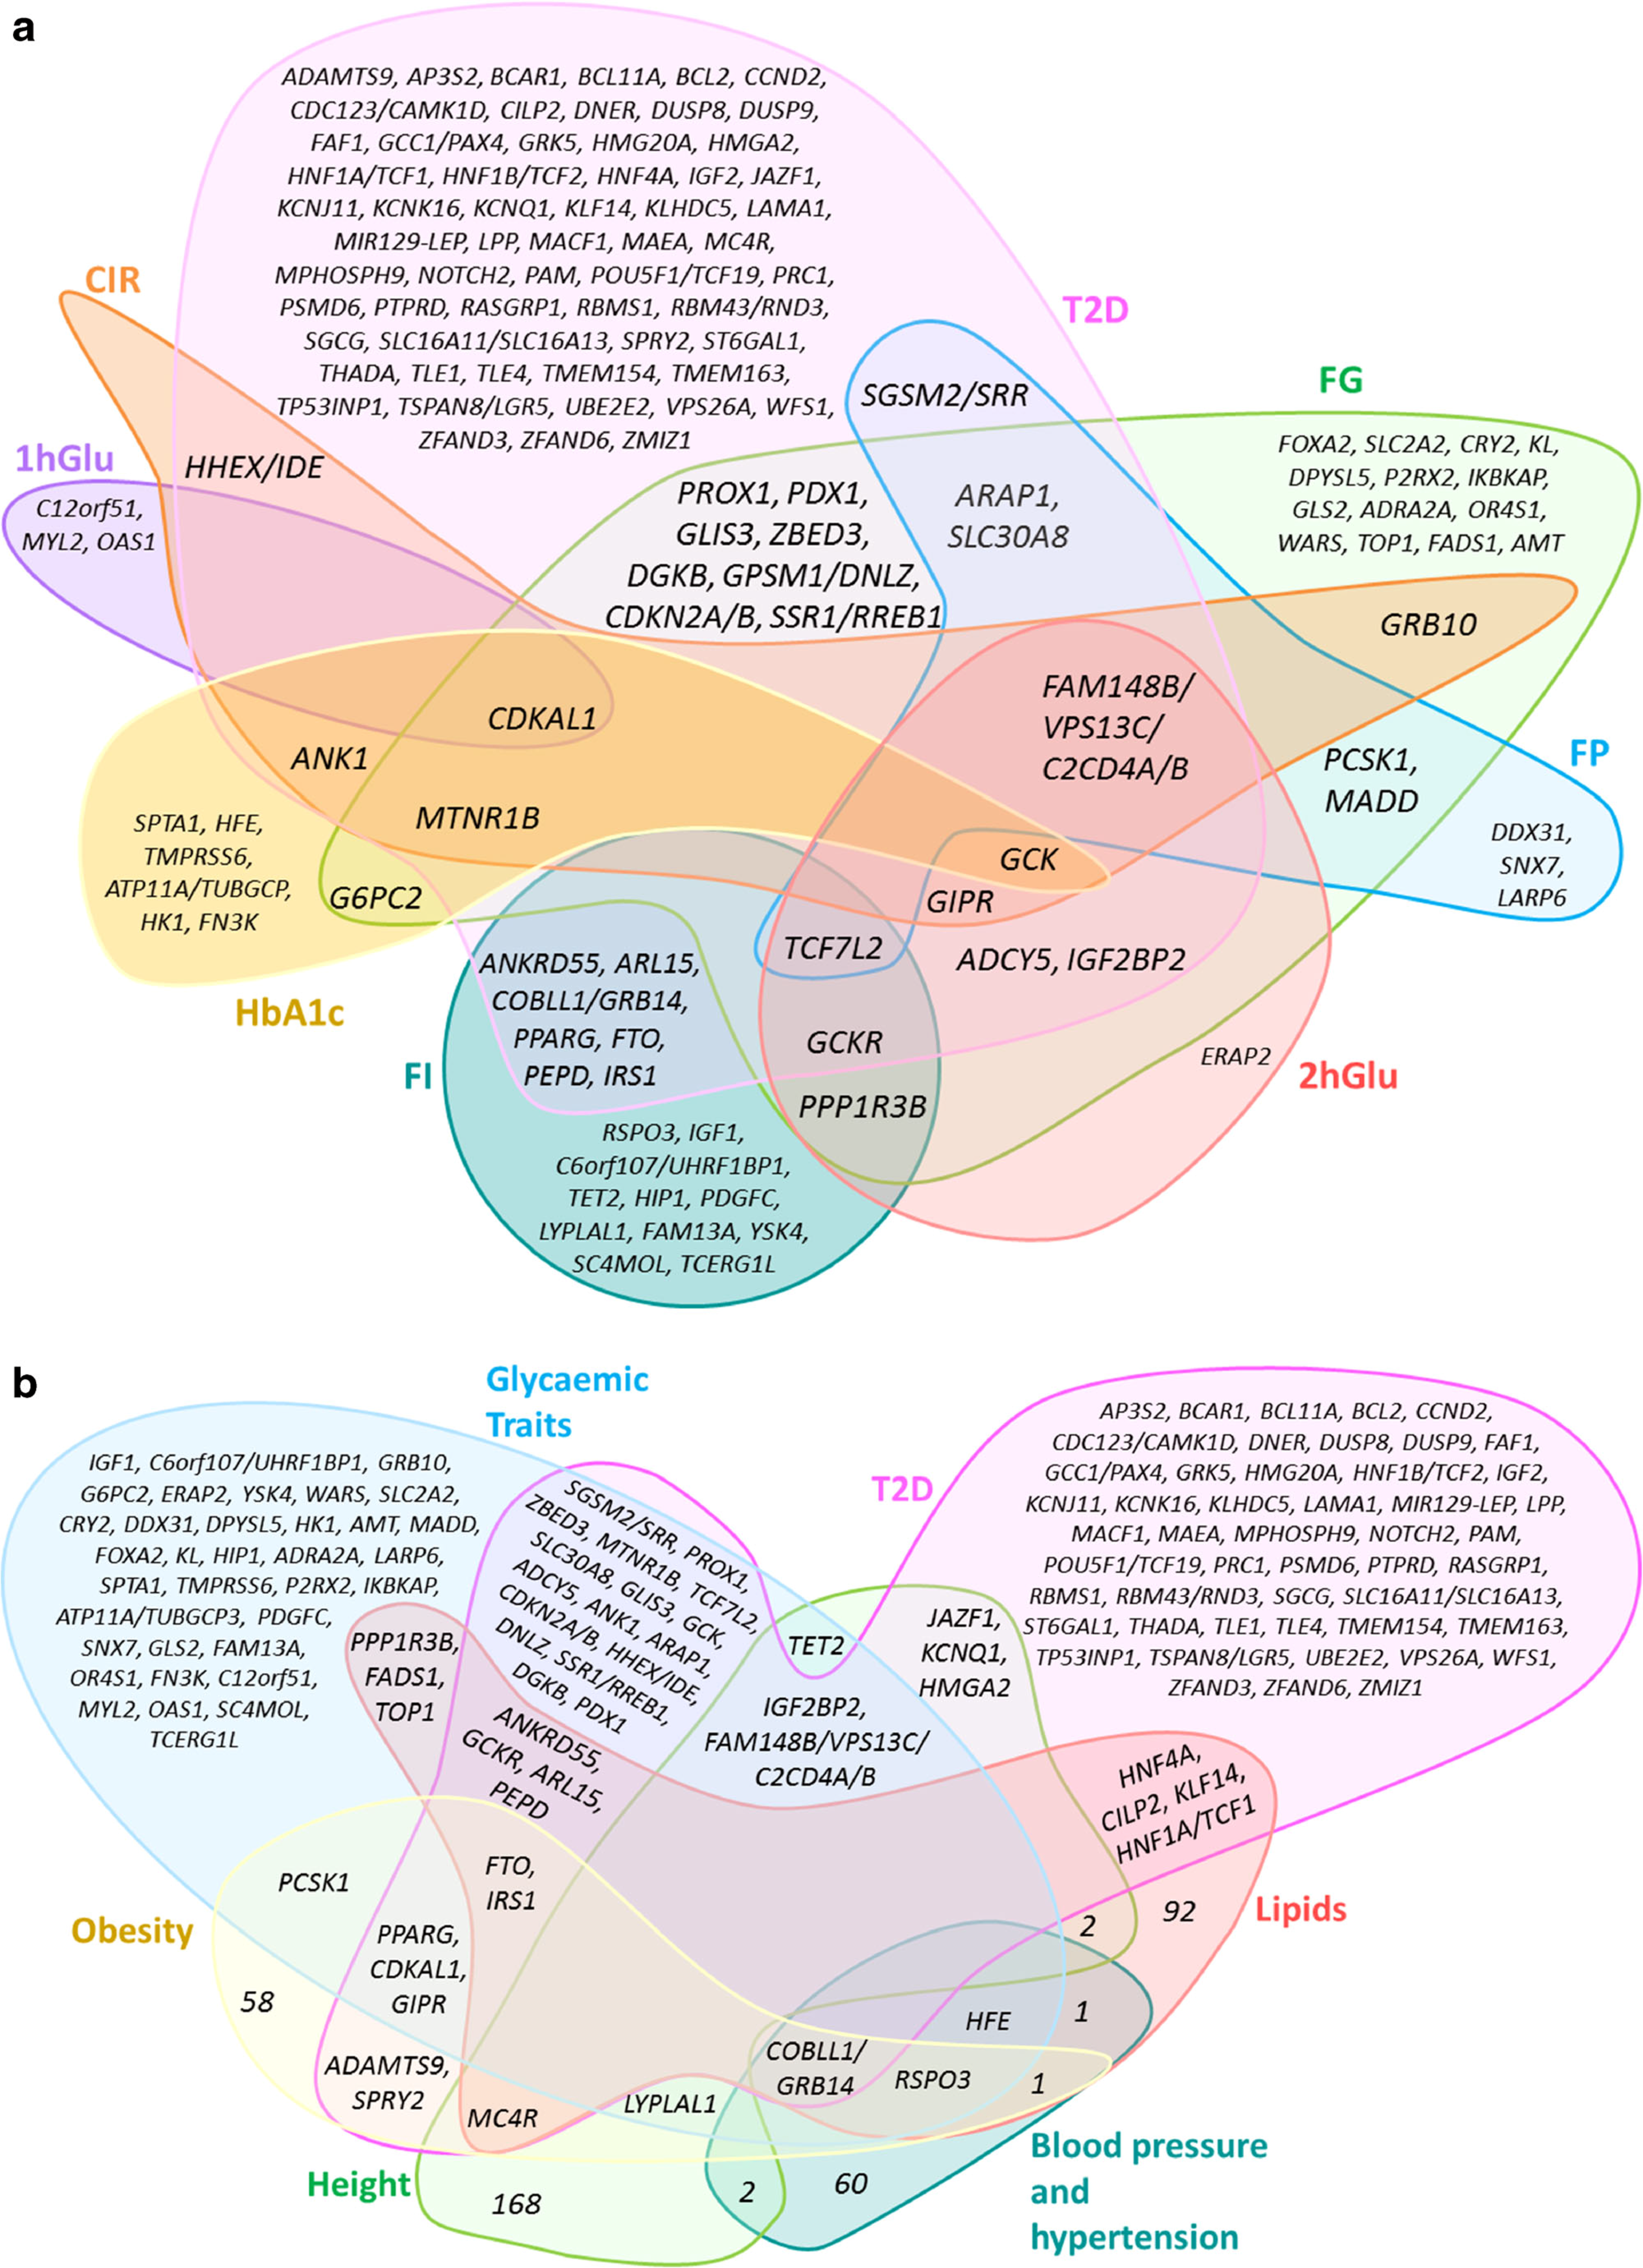
\includegraphics[width=6in]{FiguresTables/ProkopenkoMetaboDiagram} 

}

\caption{Diagramme de Venn des loci identifiés par
études d'association pangénomiques pour leur effet sur différents traits
glycémiques et le diabète de type 2 \citep{marullo_insights_2014}. T2D~:
diabète de type 2~; FG~: glycémie à jeun~; FI: insulinémie à jeun~; FP~:
proinsulinémie à jeun~; 2hGlu~: glycémie à 2 heures~; HbA1c~:
hémoglobine glyquée~; CIR~: ratio carbohydrate-insuline.}\label{fig:ProkopenkoMetaboDiagram}
\end{figure}

Au cours de la dernière décennie, et depuis la première étude
d'association pangénomique (``Genome-Wide Association Study'' ou GWAS)
portant sur le diabète de type 2 \citep{sladek_genome-wide_2007}, à
l'heure actuelle, plus de 100 loci ont été identifiés (Figure
\ref{fig:T2Dhistory}) comme étant associés au diabète de type 2, dont
certains sont également associés à la glycémie ou l'insulinémie dans des
populations normoglycémiques (Figure \ref{fig:ProkopenkoMetaboDiagram}),
notamment les gènes \emph{MTNR1B} (``Melatonin Receptor 1B'')
\citep{bouatia-naji_variant_2009, prokopenko_variants_2009, sladek_genome-wide_2007, tam_common_2010}
et \emph{TCF7L2} (``Transcription Factor 7-Like 2'')
\citep{grant_variant_2006, groves_association_2006, zhang_variant_2006}.





\begin{figure}[!htb]

{\centering 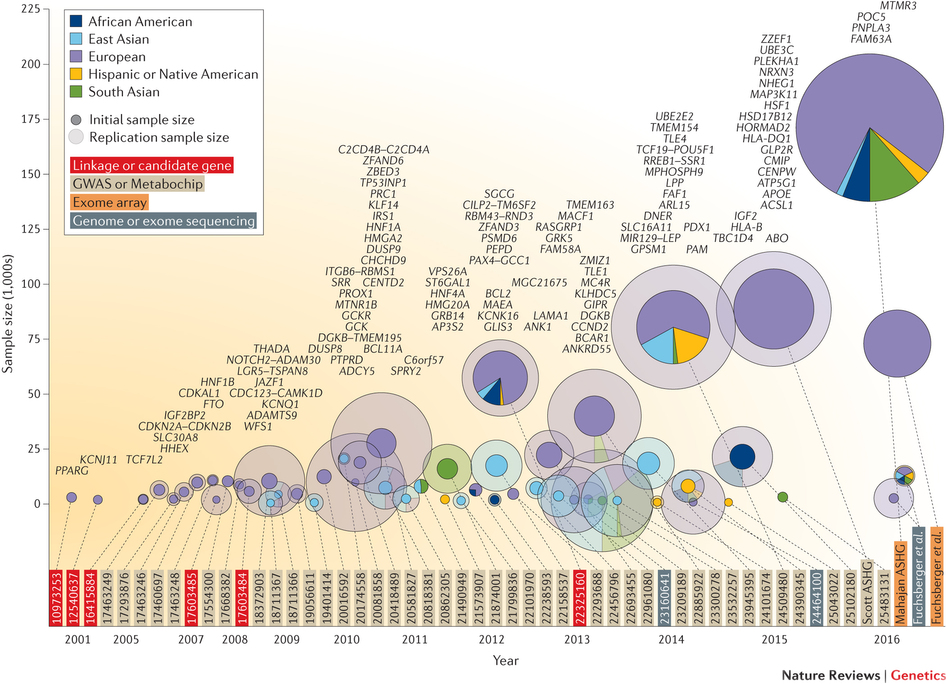
\includegraphics[width=6in]{FiguresTables/T2Dhistory} 

}

\caption{Historique des loci de susceptibilité au diabète de
type 2 identifiés par études d'association pangénomiques
\citep{flannick_type_2016}.}\label{fig:T2Dhistory}
\end{figure}

Les études ayant mené à l'identification de ces variants regroupent des
études de liaison et des études d'association de type gènes-candidats.
Par exemple, en utilisant la puce Illumina Metabochip
\citep{voight_metabochip_2012} qui inclut environ 200~000 variants
préalablement sélectionnés de résultats provenant des études
d'association sur des traits métaboliques, cardiovasculaires et
anthropométriques, environ 5~000 variants susceptibles d'être associés
au diabète de type 2, et 17~000 autres dans des régions déjà associées
dans des études antérieures (par GWAS ou séquençage du génome) ont été
testés.\\
Il est à noter que les loci identifiés par GWAS et par meta-analyses
présentent, en premier lieu, des effets observés faibles sur le diabète
de type 2 (odds ratio compris entre 1,1 et 1,4) et ne contribuent que
faiblement à l'héritabilité de cette pathologie (10 à 15~\%)
\citep{scott_genome-wide_2007, morris_large-scale_2012}. Ces estimations
de l'héritabilité ont conduit à l'émergence d'un débat portant sur
``l'héritabilité manquante'', ouvrant la voie vers de nouvelles pistes
de recherches comme, par exemple, le séquençage de l'ensemble de l'exome
ou du génome dans le but d'étudier des variants avec de faibles
fréquences alléliques, et l'étude des CNV
\citep{manolio_finding_2009}.\\
La localisation intergénique ou intronique de ces loci ne permet pas
d'identifier la fonction de ces variants de façon évidente, à quelques
exceptions près, comme par exemple les loci au niveau de \emph{GCKR}
(``glucokinase regulatory protein'') et \emph{SLC30A8} (``ZnT-8 zinc
transporter''), qui entraînent une altération de la séquence codante du
transcrit de ces gènes
\citep{beer_p446l_2009, mccarthy_genome-wide_2009, saxena_genome-wide_2007, sladek_genome-wide_2007}.

La problématique de l'héritabilité manquante a renforcé l'hypothèse de
``maladie commune, variants rares'', laquelle stipule que des variants
rares pourraient avoir une pénétrance plus forte et un effet plus
important sur le risque de diabète de type 2 que les variants communs
\citep{lupski_clan_2011, schork_common_2009}. Cette hypothèse fait
contrepoids à l'hypothèse présupposée des études gènes-candidats et des
GWAS, c'est-à-dire celle de ``maladie commune, variant commun''
\citep{schork_common_2009}. Un variant commun est un variant dont la
fréquence allélique est supérieure à 5~\% dans la population générale,
ce qui représente le seuil standard pour analyse statistique des SNPs
dans les GWAS.

Ces études d'associations ont pu mettre en évidence le fait que certains
variants pouvaient avoir un effet sur le risque de diabète de type 2,
mais également avoir un effet sur des traits cliniques, telles
l'insulinémie ou la glycémie
\citep{dupuis_new_2010, voight_twelve_2010, yaghootkar_recent_2013}. Il
est à noter qu'en raison de la prise de traitement influençant la
glycémie et l'insulinémie, les études réalisées sur ces traits ne l'ont
été que chez des individus normoglycémiques (non diabétiques). De plus,
les variants présentant un effet à la fois sur la glycémie et sur le
risque de diabète de type 2 ne représentent qu'une faible proportion des
variants identifiés
\citep{dupuis_new_2010, voight_twelve_2010, yaghootkar_recent_2013}.
Cela indique que les mécanismes conduisant au diabète de type 2 et à
l'élévation de la glycémie ne sont pas les mêmes, et paradoxalement
qu'une élévation de la glycémie chez un individu pourrait ne pas
augmenter son risque de développer un diabète de type 2.

L'épigénétique, principalement la méthylation de l'ADN et les
modifications d'histones, est devenue une composante importante dans
l'étude de la pathogenèse du diabète de type 2. En effet, ces
modifications n'altèrent pas la séquence d'ADN et peuvent être
transmises de génération en génération \citep{raciti_personalized_2014}.
Elles sont également le reflet de facteurs environnementaux et peuvent
modifier l'expression, voire activer ou éteindre complètement certains
gènes \citep{zierath_research_2011}. Dans un sens, ces modifications
peuvent avoir un effet équivalent aux SNPs ou à d'autres mutations, en
bloquant la transcription d'un gène. Plusieurs éléments viennent
corroborer l'idée selon laquelle l'épigénétique pourrait expliquer une
partie de ``l'héritabilité manquante'' dans le diabète de type 2,
notamment en tant que reflet de l'environnement intra-utérin, comme cela
a été montré dans des populations soumises à des contraintes
alimentaires, où le risque de développement d'un diabète de type 2 était
accru chez les enfants dont la mère avait connu une famine au moment de
la grossesse
\citep{hales_type_1992, pettitt_congenital_1988, ravelli_glucose_1998}.
Des études similaires menées chez les indiens Pima ont montré des
risques de développement de diabète supérieurs chez l'enfant lorsque la
mère présentait une hyperglycémie et/ou un diabète
\citep{dabelea_intrauterine_2000, pavkov_effect_2010, pettitt_excessive_1983}.

Une autre indication vient de l'étude des perturbateurs endocriniens et
de polluants qui sont présents sous différentes formes dans divers
produits et outils de la vie de tous les jours (p.~ex. boîte alimentaire
en plastique, produits d'entretien, peintures, etc.). Ces substances
peuvent avoir un effet sur la méthylation de l'ADN, résultant en un
changement coordonné de l'expression des gènes (mRNA, miRNA), et ainsi
produire un effet sur la sécrétion d'insuline \citep{hall_effects_2014}
ou l'homéostasie du glucose, comme cela a été observé chez l'homme
\citep{bi_diabetes_2015} et chez les rongeurs (rat et souris)
\citep{li_f0_2014, rajesh_gestational_2015}. En raison du caractère
tissu-spécifique de la méthylation, les premières études se sont
focalisées sur les tissus dont les échantillons étaient facilement
prélevables, tels que le sang
\citep{bell_integrated_2010, canivell_differential_2014, chambers_epigenome-wide_2015, dayeh_dna_2016, toperoff_genome-wide_2012}
et le pancréas, notamment les îlots pancréatiques impliqués dans la
sécrétion d'insuline
\citep{dayeh_genome-wide_2014, hall_effects_2014, stitzel_global_2010, volkmar_dna_2012}.
Dans l'une des premières études de l'épigénome à grande échelle via
l'utilisation de puce Illumina HumanMethylation450 BeadChip
(\textasciitilde{}480~000 sites CpG couverts), plus de 1~600 CpG
(\textasciitilde{}850 gènes), incluant des loci connus tels que
\emph{TCF7L2} et \emph{KCNQ1}, ont été identifiés comme étant
différentiellement méthylés entre des diabétiques et des non diabétiques
\citep{dayeh_genome-wide_2014}. Des études plus récentes ont apporté des
pistes de réponse, quant à la nature causale de la méthylation, en
considérant les polymorphismes identifiés dans le diabète de type 2
(Consortium DIAGRAM) \citep{morris_large-scale_2012}. Ainsi, la
méthylation du locus KCNQ1 serait causale dans le développement du
diabète de type 2 \citep{elliott_role_2017}.

Bien que l'ère des GWAS ait permis d'identifier plus de 100 loci
associés au diabète de type 2, les mécanismes liant ces variants à sa
pathogenèse restent méconnus pour une grande partie d'entre eux. À cela
s'ajoute que ces variants ne constituent qu'une faible part de
l'héritabilité de cette maladie complexe. Ainsi, au cours des dernières
années, les axes de recherches se sont progressivement déplacés vers
l'étude d'autres ``-omiques'' comme la transcriptomique, l'épigénomique,
ou encore la métabolomique. La grande diversité des organes/tissus
impliqués dans la pathogenèse du diabète de type 2 renforce la nécessité
de recueillir et d'étudier en détail le caractère spécifique des tissus
et la fonction des cellules qui les composent, afin de pouvoir établir
une carte détaillée des mécanismes sous-jacents au développement du
diabète de type 2. Avec le développement des techniques et technologies,
il est également possible non seulement d'étudier séparément la
génétique, l'épigénétique et les facteurs environnementaux afin de
classer les individus selon leur risque de développer un diabète, mais
aussi d'étudier les interactions et les connections entre ces
différentes composantes. Les études fonctionnelles représentent
également une étape importante dans la compréhension des mécanismes
biologiques des loci identifiés à l'aide des études ``-omiques''. La
variété et la croissance de la quantité des données générées nécessitent
un développement constant d'outils et de méthodes statistiques visant à
identifier des gènes ou loci candidats. L'intégration des différentes
données ``-omiques'' offre la possibilité de mettre au jour de nouvelles
connaissances sur la chronologie des mécanismes en amont et en aval du
développement d'une pathologie, mais également de révéler les liens
unissant le génome et le phénome.

\section{Méthodes statistiques : des données à la
biologie}\label{methodes-statistiques-des-donnees-a-la-biologie}

\subsection{La statistique génétique}\label{la-statistique-genetique}

Les principes de l'héritabilité développés par Gregor Mendel (1822-1884)
à la fin du XIXème siècle ont servi de fondements à la plupart des
connaissances actuelles sur la transmission des traits des parents à
leurs enfants. Au fur et à mesure du développement du concept de traits
hérités s'est développée la génétique, la science qui étudie la
transmission de ces traits et du matériel biologique dans les organismes
vivants. La génétique est devenue partie intégrante de la recherche sur
l'origine de certaines maladies, comme l'obésité et le diabète.
Contrairement à l'étude des végétaux et des petits animaux (rat, souris,
etc.), où la croissance et les croisements peuvent être contrôlés de
façon expérimentale, et où la transmission des caractères étudiés est
rendue possible dans un temps limité (en particulier grâce à un temps
réduit de passage d'une génération à la suivante, p.~ex. 2-4 mois pour
le poisson-zèbre), la situation est plus complexe chez l'Homme,
puisqu'il faut entre 20 et 30 ans pour qu'une nouvelle génération voit
le jour.

Aujourd'hui, avec les évolutions technologiques au niveau des
plateformes moléculaires, ayant notamment permis le séquençage du génome
humain (``Human Genome Project'' \citep{sawicki_human_1993}), le volume
des données génomiques a augmenté au cours des dernières décennies et a
ainsi permis le développement d'une branche de la statistique, soit la
statistique génétique. Cette nouvelle branche vise à développer des
outils d'analyses des caractères hérités et plus généralement des
données génétiques, permettant en outre l'identification de facteurs de
risque ou de déterminants génétiques pour des maladies complexes, tels
que les cancers, les diabètes, les maladies cardio-vasculaires ou les
troubles psychiatriques. Une maladie complexe est définie comme une
pathologie dont les causes sont multiples, lesquelles peuvent être le
fruit d'une interaction de facteurs comportementaux, environnementaux et
génétiques pouvant produire un effet sur plusieurs gènes de façon
simultanée. Ces maladies complexes s'opposent aux maladies dites
mendéliennes, dont l'origine s'explique principalement par la génétique,
via des processus de transmission conjecturés par Gregor Mendel. Ces
maladies se caractérisent par la transmission d'un gène délétère à la
descendance, comme c'est le cas pour les formes de diabète MODY
discutées précédemment.

\subsection{Recueil et prétraitement des
données}\label{recueil-et-pretraitement-des-donnees}

\subsubsection{Puce-à-ADN}\label{puce-a-adn}

L'émergence des puces à ADN (``DNA micro-array''), notamment propulsées
par les grands projets internationaux de séquençage tels le ``Human
Genome Project'' \citep{sawicki_human_1993}, ``HapMap Project''
\citep{gibbs_international_2003}, ``1~000 Genomes Project''
\citep{siva_1000_2008, the_1000_genomes_project_consortium_global_2015},
a permis d'étendre le champ d'application de la statistique grâce à la
disponibilité et la variété des données issue de ces puces, à savoir
aussi bien des données de transcriptomique, de génomique et
d'épigénomique. En effet, les puces à ADN utilisent le principe
d'hybridation de l'ADN reposant sur la complémentarité de ces bases.
Rappelons le fonctionnement des puces à ADN d'un point de vue général.



\begin{figure}[!htb]

{\centering 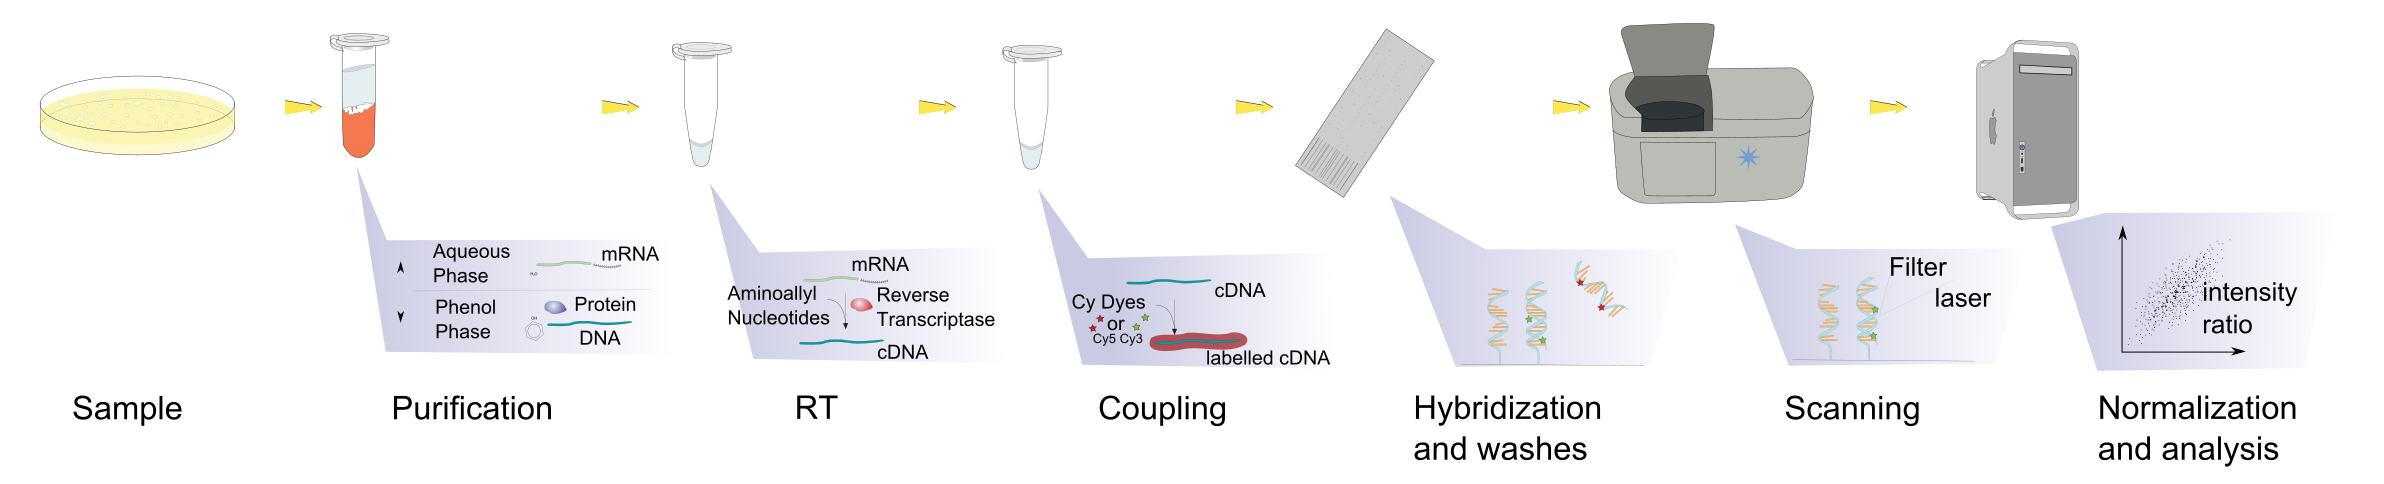
\includegraphics[width=6in]{FiguresTables/Microarray} 

}

\caption{Schéma du protocole des puces à ADN.}\label{fig:Microarray}
\end{figure}

L'ADN est extrait et purifié à partir d'un échantillon de tissu (p.~ex.
prélèvement sanguin ou salivaire). L'ADN purifié peut ensuite être
amplifié au moyen d'une réaction en chaîne par polymérase (PCR), un
procédé qui permet d'augmenter la quantité d'ADN. Un marquage des
séquences par le remplacement de certaines bases nucléotidiques par leur
analogue radioactif est ensuite réalisé. Les séquences d'ADN marquées
sont ensuite hybridées sur des sondes spécifiques disposées sur les
puces à ADN, puces pouvant contenir des milliers de ces sondes
complémentaires de séquences d'ADN. Une fois l'hybridation des séquences
d'intérêts réalisée, la puce est passée dans un outil de visualisation
permettant de lire et quantifier la fluorescence émise par chaque puits
(position d'une sonde sur la puce). Selon le type d'omique, le protocole
utilisé dans les puces varie et peut inclure des étapes spécifiques,
telles qu'une étape de conversion de l'ARN en cDNA (ADN complémentaire
de l'ARN reconstitué par une étape de transcription inverse) pour une
étude transcriptomique, ou bien une étape de bisulfitation dans le cas
d'une étude méthylomique, permettant le changement de la cytosine
non-méthylée d'un groupement CpG en uracile avant de passer à l'étape
d'amplification PCR. C'est à l'issue de ces étapes (Figure
\ref{fig:Microarray}), que l'information génomique, transcriptomique ou
méthylomique est disponible sous forme de données numériques pouvant
être analysées après un prétraitement et un contrôle-qualité.

\subsubsection{Prétraitement}\label{pretraitement}

Comme dans toute analyse statistique, la validité des résultats est
conditionnée par la qualité des données. De ce fait, une étape de
contrôle de qualité et de plausibilité des données est indispensable. En
plus des problématiques génériques telles que les valeurs extrêmes, les
études omiques soulèvent quelques niveaux de complexité supplémentaires
provenant en grande partie des protocoles complexes générant ces
données. Ainsi, dans le cas du génotypage, la qualité peut être
influencée par plusieurs facteurs n'étant pas toujours sous contrôle,
comme la qualité de l'ADN qui dépend du type de prélèvement de
l'échantillon (p.~ex. échantillon sanguin ou buccal, biopsie, etc.), le
stockage et la conservation de l'échantillon (p.~ex. température,
stockage paraffine, etc.), et la plateforme de génotypage (c.-à-d. la
technologie utilisée par le manufacturier).

\paragraph{Génomique}\label{genomique}

Dans les études populationnelles, les erreurs de génotypage survenant
indépendamment du statut des individus (p.~ex. malade/non malade) ou de
leur génotype, peuvent occasionner une diminution de la puissance
statistique sans pour autant modifier le risque de première espèce des
tests
\citep{fardo_quality_2009, gordon_assessment_2001, marquard_impact_2009},
ce qui peut ne pas être le cas dans les études familiales où le taux de
faux positifs peut alors être augmenté
\citep{yan_impact_2016, abecasis_impact_2001}. Cette diminution de la
puissance statistique et augmentation de l'erreur de type 1 sont
d'autant plus importantes lorsque les erreurs de génotypage se trouvent
être associées aux génotypes et/ou phénotypes, voire au plan
expérimental (c.-à-d. différents techniciens, séparation complète des
groupes étudiés sur des puces différentes, etc.). Une étape de
contrôle-qualité peut consister en l'application de plusieurs filtres
successifs, en particulier au moyen du logiciel PLINK
\citep{chang_second-generation_2015, purcell_plink_2015}qui dispose de
nombreuses fonctionnalités pour la manipulation de fichiers génomiques.
Ces filtres peuvent être regroupés en deux catégories, d'une part sur
les individus, et d'autre part sur les variants génétiques.

\subparagraph{Contrôle-qualité des échantillons}\label{QCgenomique}








\begin{figure}[!htb]

{\centering 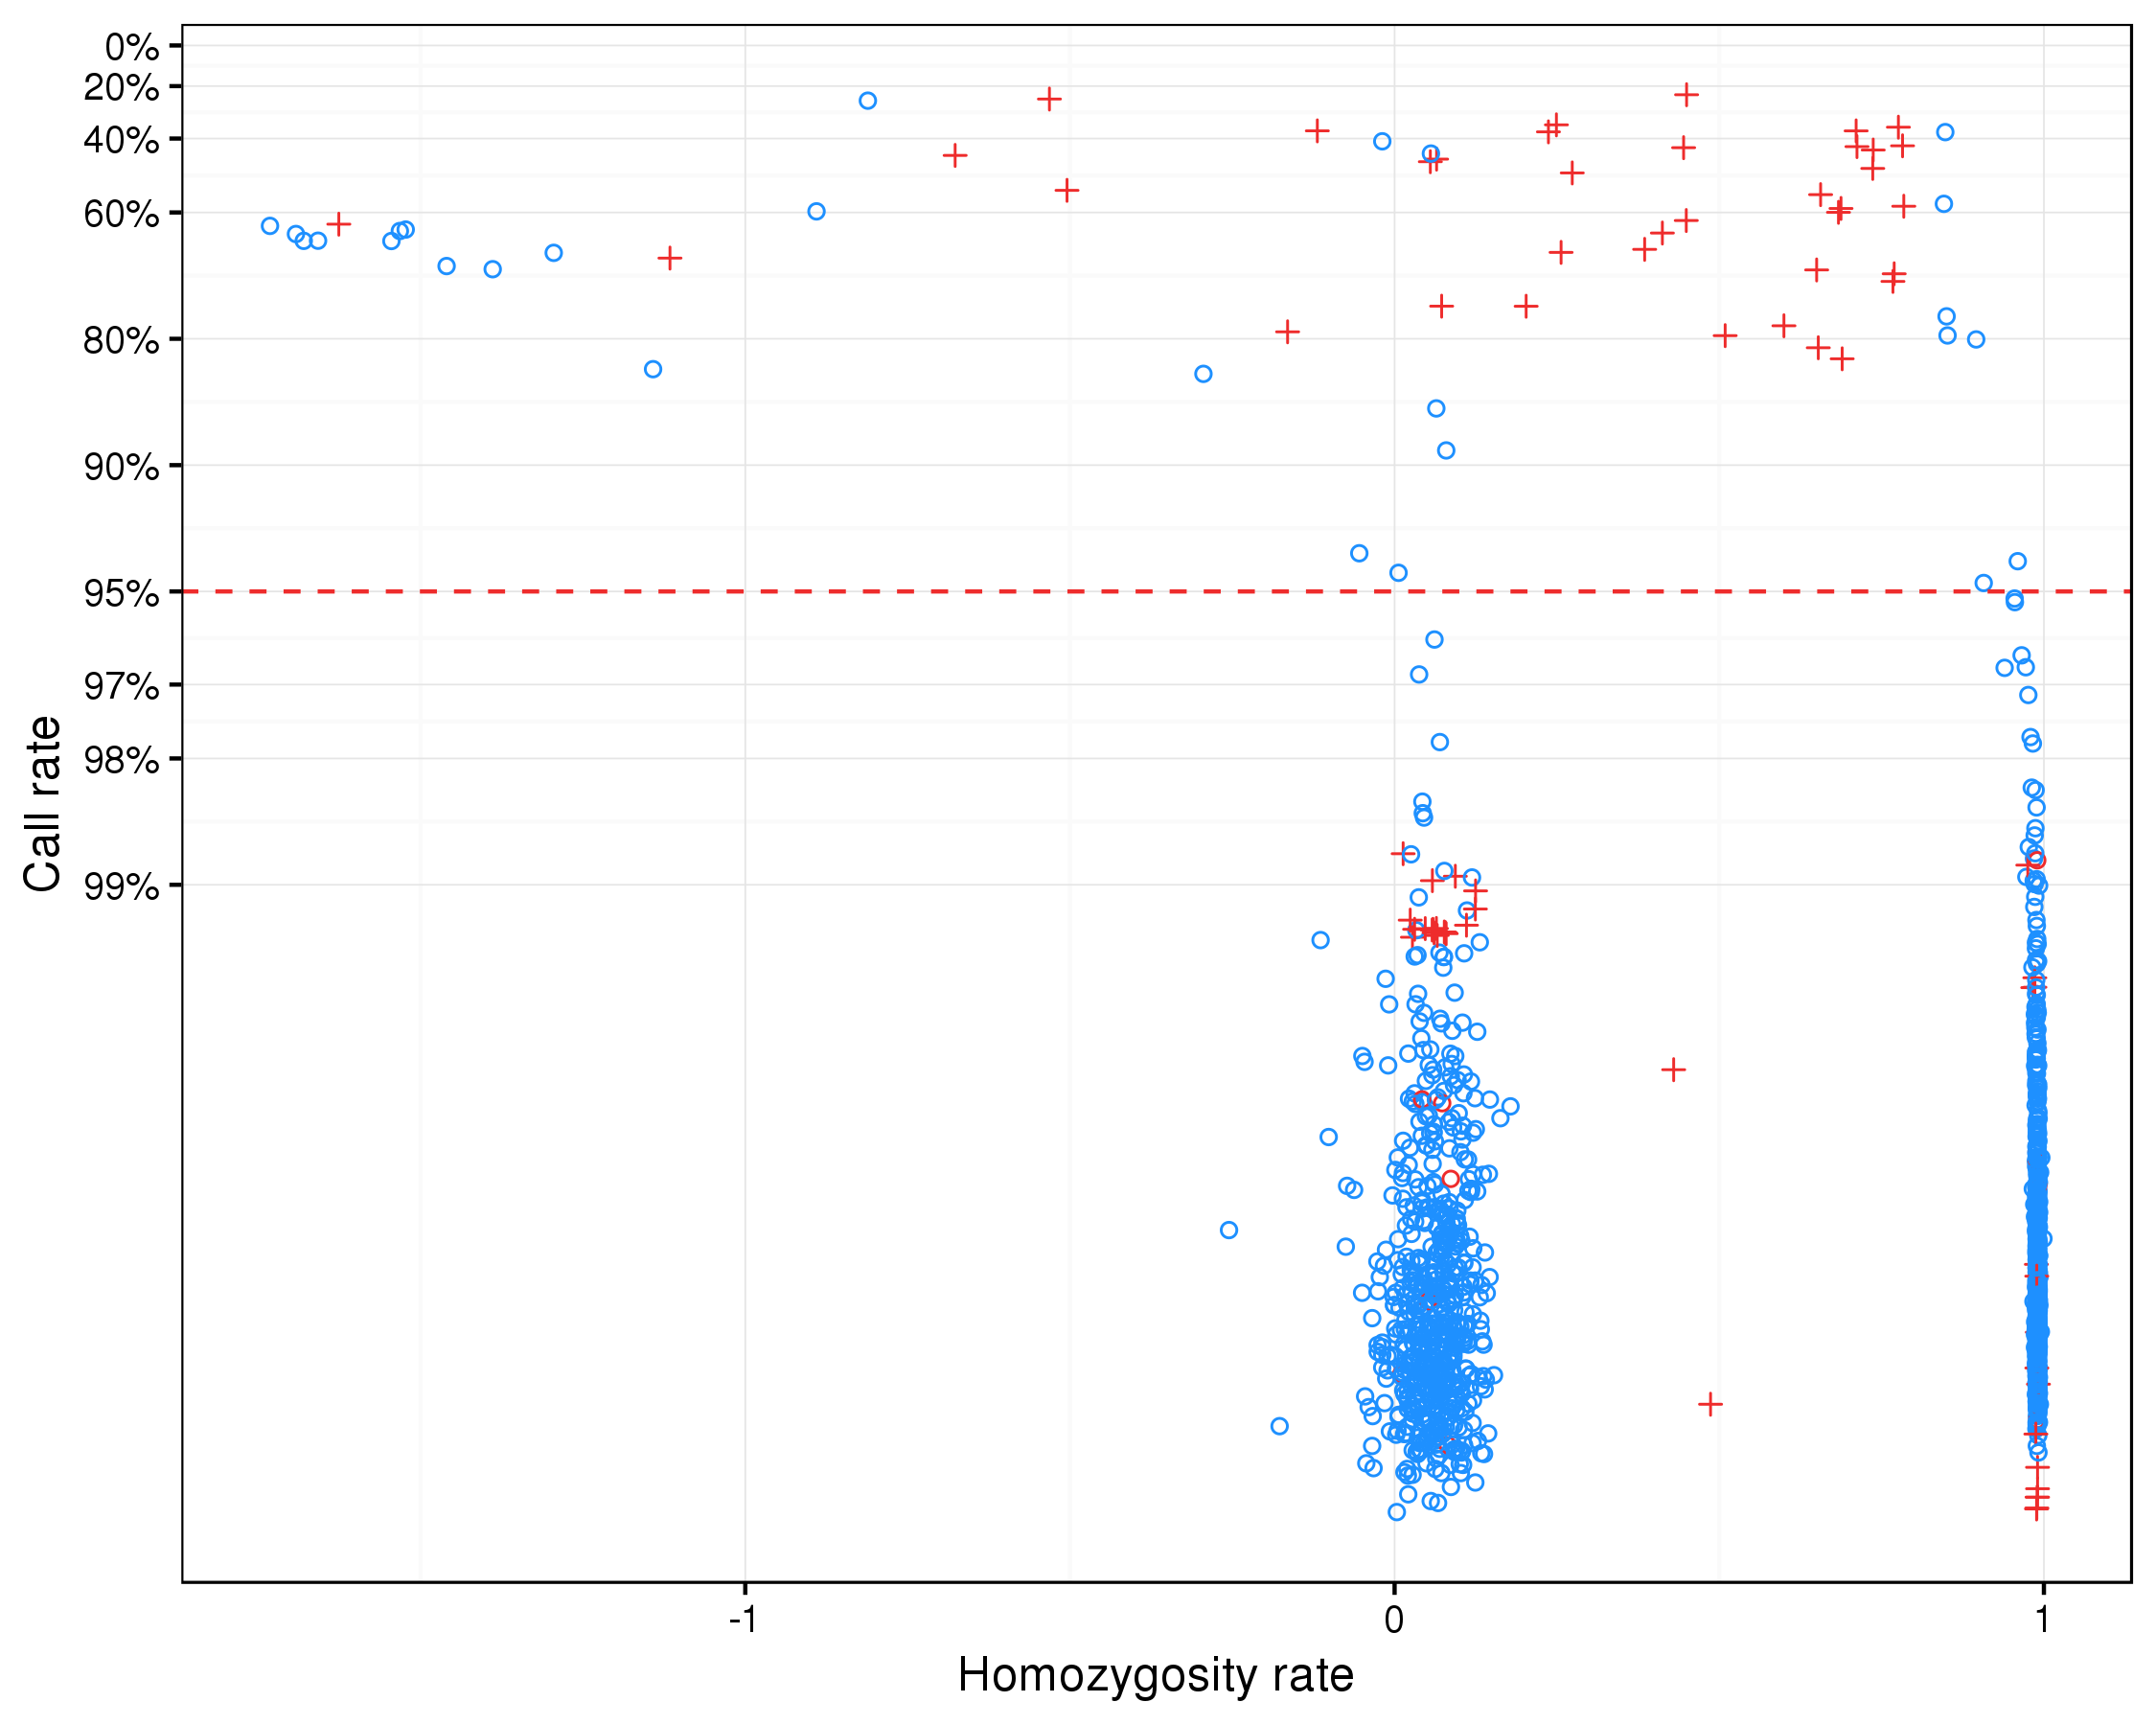
\includegraphics[width=3in,height=2.4in]{FiguresTables/gendercheck} 

}

\caption{Le taux d'homozygotie (estimé à l'aide des variants du
chromosome X) est représenté en fonction de la proportion de génotypes
manquants par échantillon. Le taux d'homozygotie attendu pour les hommes
est de 1 et inférieur à 0,2 pour les femmes. Les points rouges
représentent les échantillons pour lesquels les informations sur le sexe
sont discordantes ou manquantes.}\label{fig:gendercheck}
\end{figure}

\begin{itemize}
\tightlist
\item
  \emph{Concordance du genre entre le génotype et le phénotype} (Figure
  \ref{fig:gendercheck})\\
  En mesurant le taux d'homozygotie au niveau des gonosomes pour chaque
  individu, il est possible de déterminer le sexe à partir du chromosome
  X. Ainsi, pour les femmes, qui présentent deux chromosomes X et
  peuvent donc avoir deux allèles différents pour chaque variant, le
  taux d'homozygotie doit être inférieur à 0,2. Pour les hommes, qui ne
  présentent qu'un seul chromosome X, le taux d'homozygotie attendu est
  de 1, ou au moins supérieur à 0,8 (seuil de tolérance). Ce filtre a
  deux objectifs~: vérifier l'information du phénotype, et fournir une
  information quant à la qualité du génotypage.
\end{itemize}




\begin{figure}[!htb]

{\centering 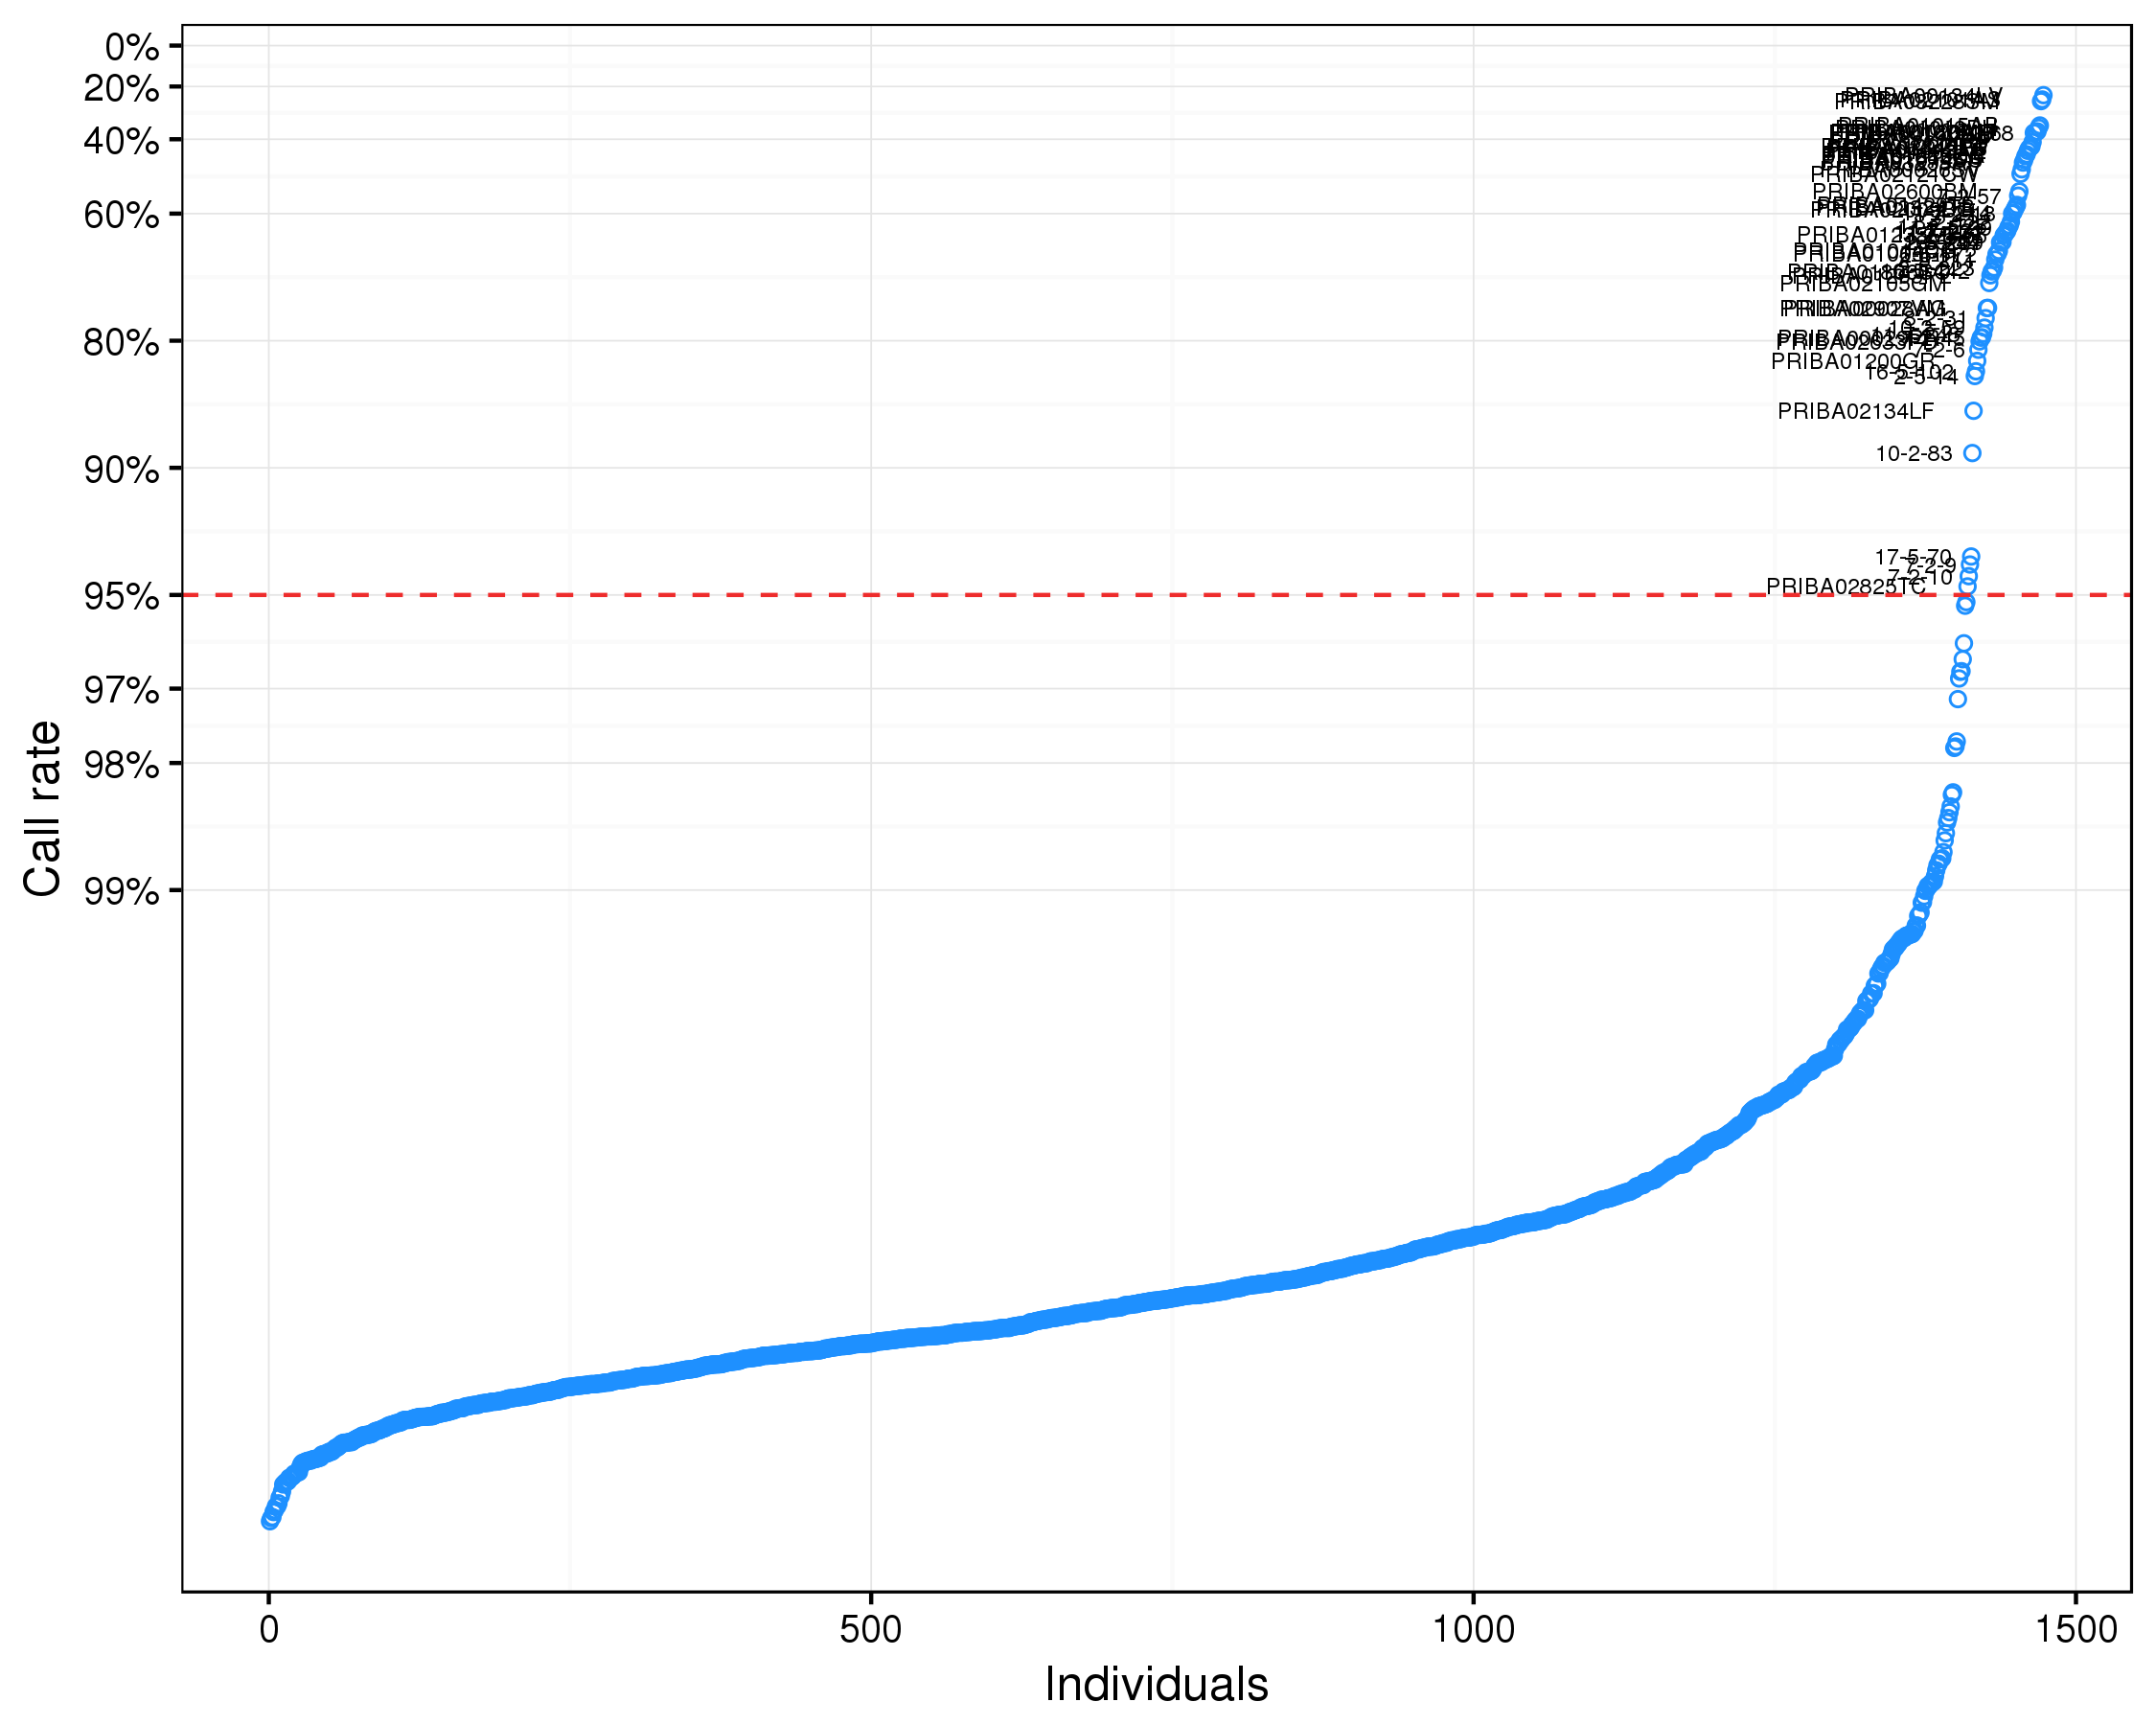
\includegraphics[width=3in,height=2.4in]{FiguresTables/samplecallrateevaluation} 

}

\caption{Distribution du taux de génotype manquant
par échantillon.}\label{fig:samplecallrateevaluation}
\end{figure}

\begin{itemize}
\tightlist
\item
  \emph{Taux de génotypage ou taux de génotype manquants} (Figure
  \ref{fig:samplecallrateevaluation})\\
  Cette vérification permet également d'identifier les individus pour
  lesquels un problème est survenu lors du génotypage ou de l'extraction
  d'ADN, en particulier un défaut de qualité de l'ADN. Les individus
  présentant plus de 5~\% de génotypes manquants sont généralement
  exclus à ce stade.
\end{itemize}









\begin{figure}[!htb]

{\centering 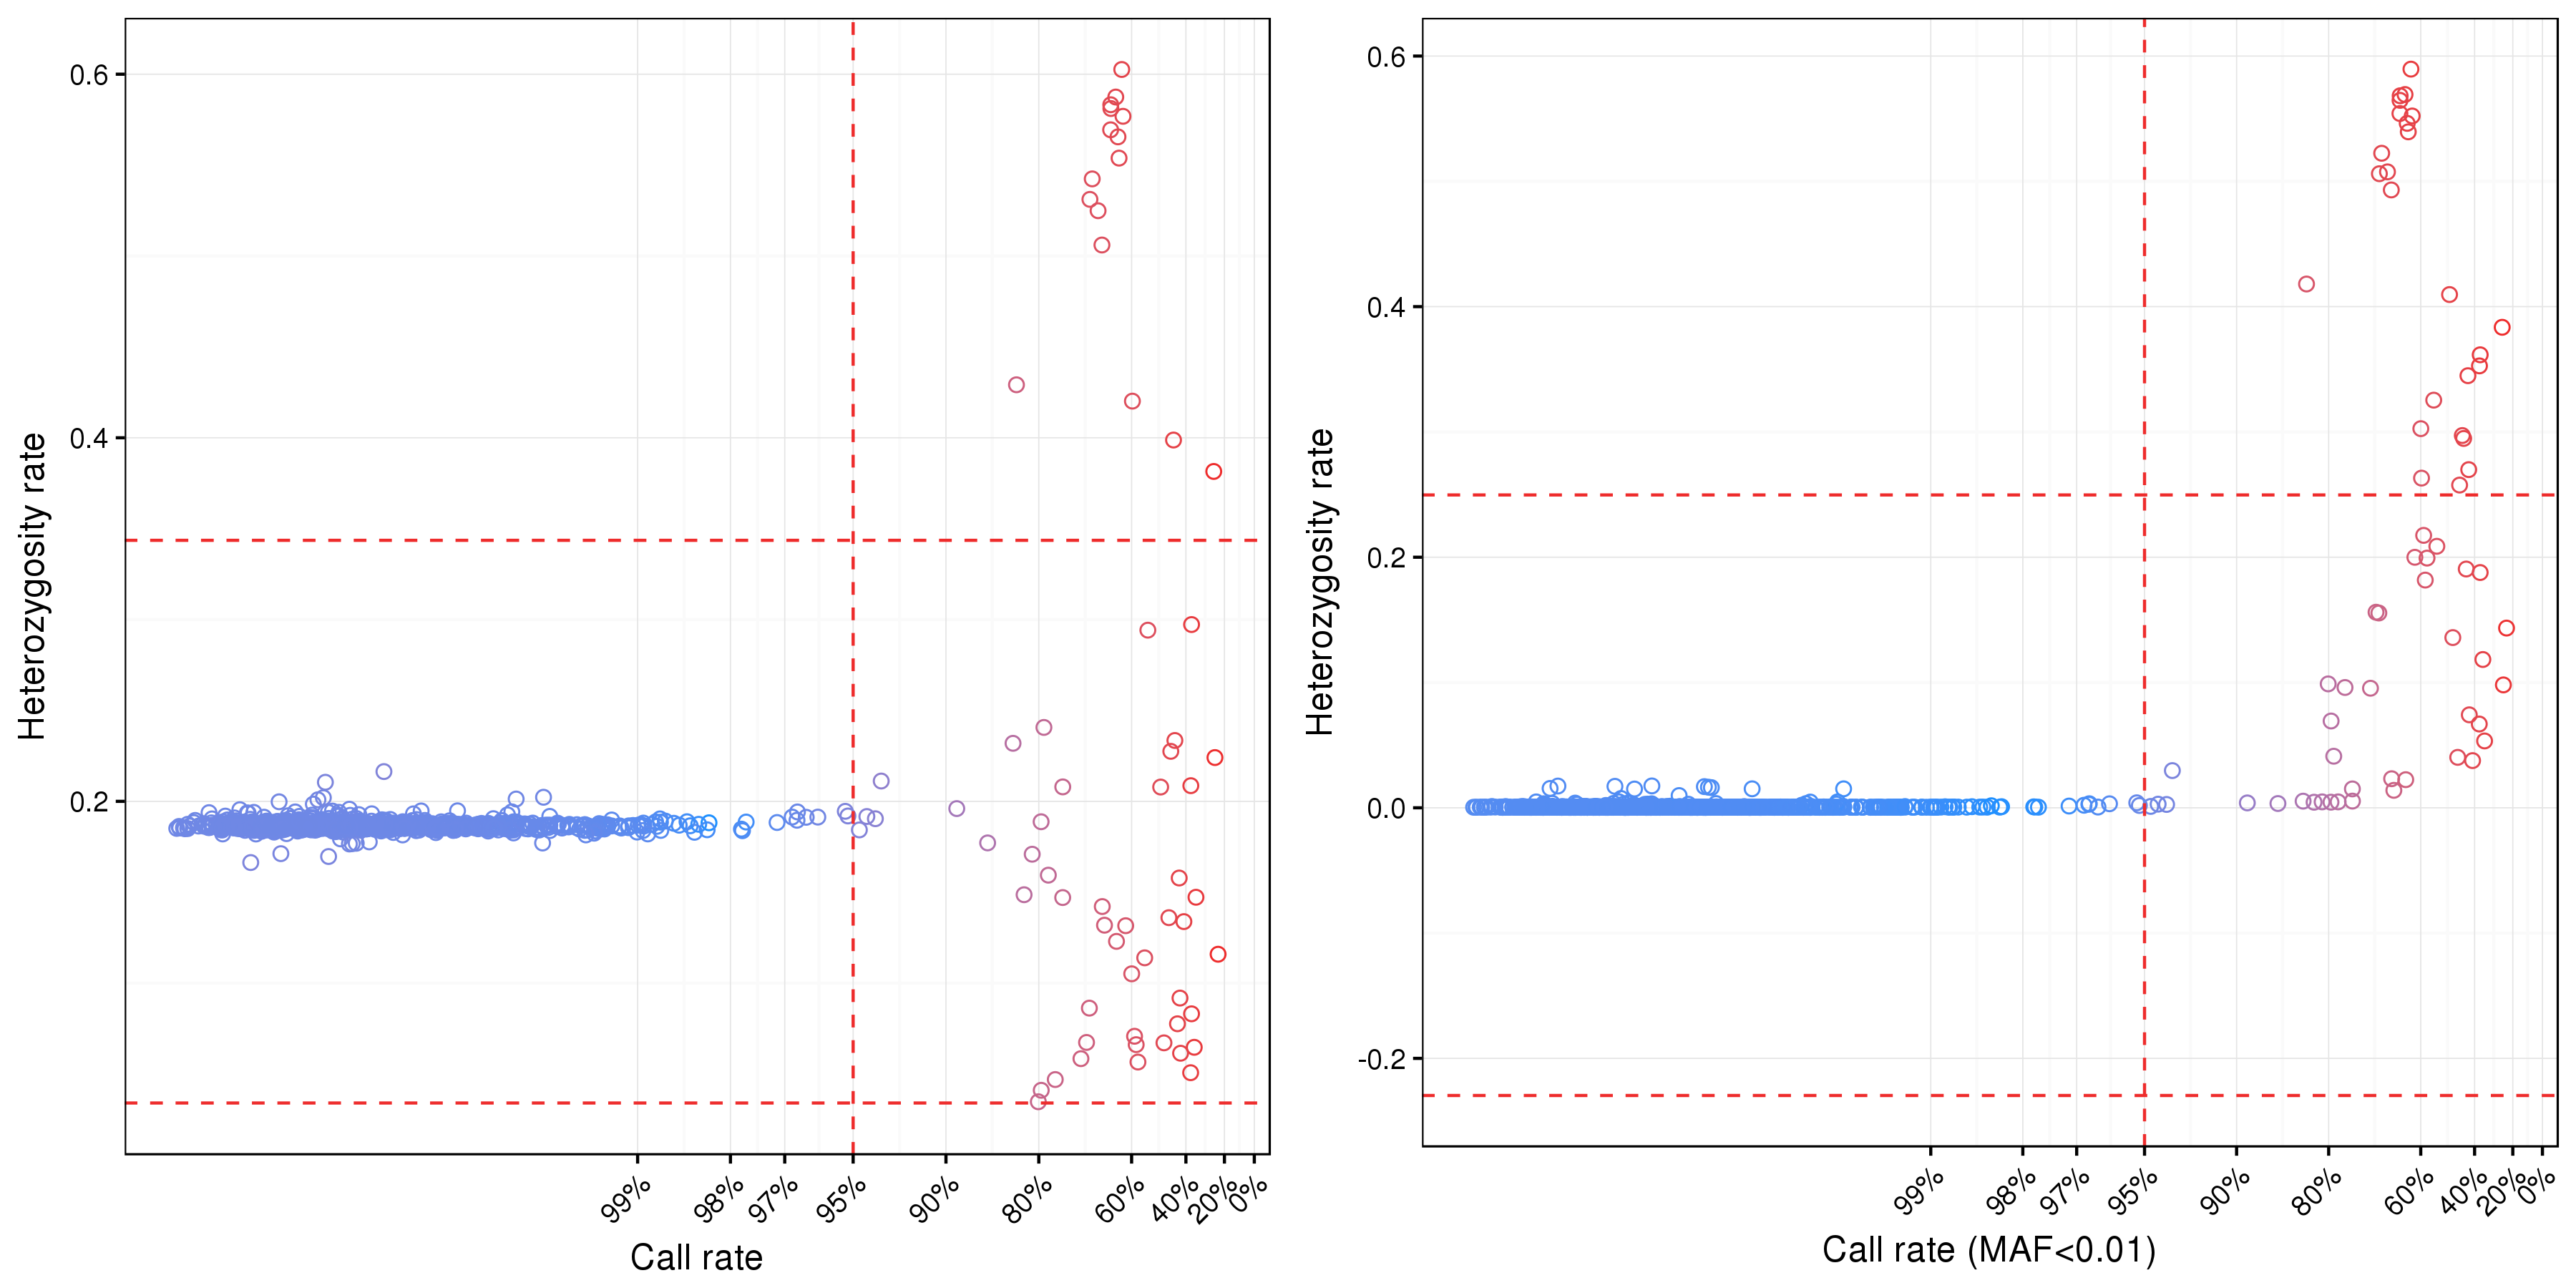
\includegraphics[width=6in,height=2.4in]{FiguresTables/heterozygositycheck} 

}

\caption{Taux d'hétérozygotie par échantillon par
rapport au taux de génotypage. À gauche, le taux d'hétérozygotie pour
l'ensemble des variants, à droite, le taux d'hétérozygotie des variants
dont la fréquence allélique est inférieure à 1~\%. Les lignes rouges
horizontales représentent l'intervalle à plus ou moins quatre fois
l'écart-type du taux moyen d'hétérozygotie. La ligne rouge verticale
indique le seuil du taux de génotypage.}\label{fig:heterozygositycheck}
\end{figure}

\begin{itemize}
\item
  \emph{Taux d'hétérozygotie (autosomes)} (Figure
  \ref{fig:heterozygositycheck})\\
  L'objectif de cette vérification est de s'assurer d'une qualité
  homogène des génotypes des individus. La distribution du taux
  d'hétérozygotie (hors chromosomes sexuels) chez tous les individus
  doit être inspectée pour identifier les individus ayant une proportion
  excessive ou réduite de génotypes hétérozygotes. En effet, cela peut
  respectivement indiquer une contamination (p.~ex. mélange de deux
  ADN), ou une consanguinité au sein des échantillons d'ADN. Les
  individus présentant un taux d'hétérozygotie extrême par rapport à la
  distribution de celui-ci sur l'ensemble des individus sont exclus,
  généralement sur la base d'un écart à la moyenne de trois à quatre
  fois l'écart-type. Le taux d'hétérozygotie (donnée par
  \(\frac{(n-h)}{n}\), où \(n\) est le nombre de génotypes total observé
  et \(h\) est le nombre de génotypes homozygotes observé pour un
  individu donné) différera selon les populations étudiées et selon
  l'ensemble des SNPs ciblés par une puce donnée.
\item
  \emph{Degré d'apparentement (étude non-familiale)}\\
  Dans le contexte des études populationnelles d'association
  pangénomiques, les individus étudiés sont sélectionnés pour satisfaire
  un critère de non-apparentement en plus de critères purement liés aux
  hypothèses auxquelles l'étude doit répondre. En effet, la présence
  d'individus apparentés (c.-à-d. du second degré ou plus proche, ou
  ayant plus de 20~\% de leur génome parfaitement identique), voire
  d'individus en doublons, peuvent introduire un biais dans l'étude par
  la surreprésentation de génotypes spécifiques à quelques familles, et
  conséquemment modifier les fréquences alléliques qui ne seront alors
  plus représentatives de la population étudiée. Pour éviter ce biais,
  le degré d'apparentement de chaque paire d'individus est mesuré à
  partir de la proportion de leurs génomes partagés avec un ancêtre
  commun (identité par descendance ou IBD). De cette façon, les
  individus en doublons ou jumeaux (monozygotes) présenteront un
  \(IBD\simeq 1\), un \(IBD\simeq 0,5\) pour les individus ayant un lien
  du premier degré (p.~ex. parents, enfants, frères et sœurs) et un
  \(IBD\simeq 0,25\) pour un lien du second degré (p.~ex. oncles,
  tantes, grand-parents, etc.). En raison d'erreur de génotypage, de
  stratification cachée dans l'échantillon (p.~ex. due à différentes
  origines ethniques) ou de déséquilibre de liaison, ces valeurs d'IBD
  théoriques peuvent varier avec des données réelles et des intervalles
  de valeurs sont alors tolérés~: par exemple, \([0,20\ ; 0,30]\) pour
  le premier degré, ou \([0,40\ ; 0,60]\) pour le second degré.
\end{itemize}






\begin{figure}[!htb]

{\centering 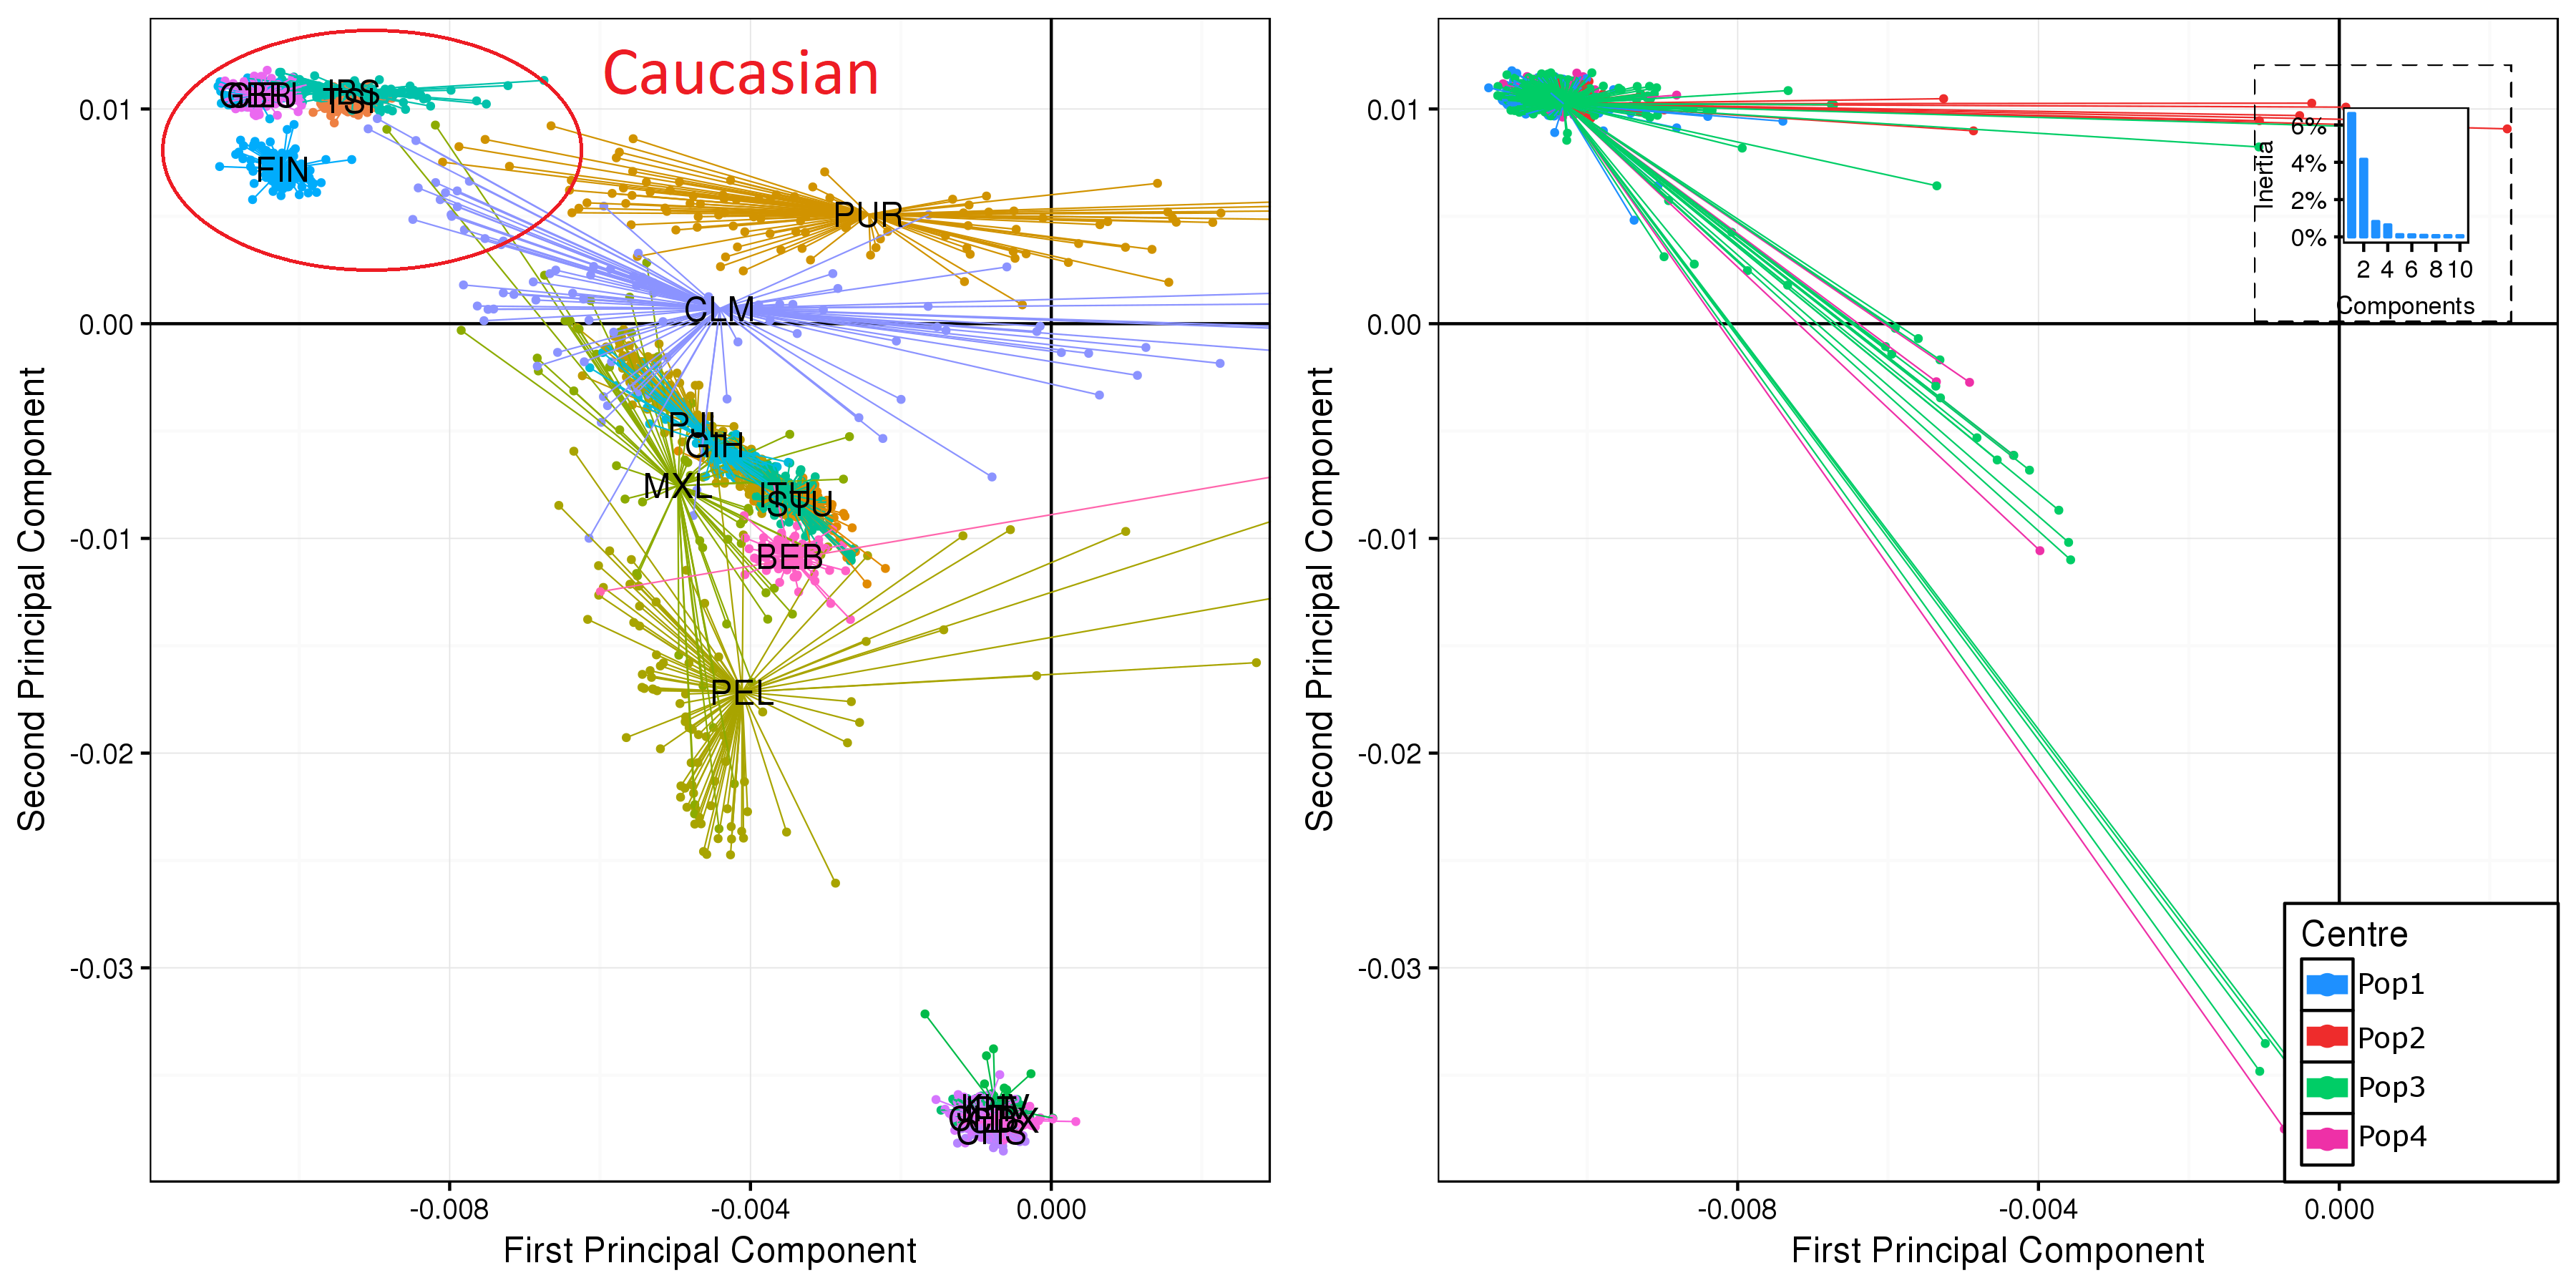
\includegraphics[width=6in,height=2.4in]{FiguresTables/population} 

}

\caption{Premier plan factoriel de l'analyse en composante
principale du jeu de données combinant la population d'étude et celle de
référence (1~000 génomes). Avec à gauche la population de référence et à
droite la population d'étude.}\label{fig:population}
\end{figure}

\begin{itemize}
\tightlist
\item
  \emph{Stratification de la population} (Figure \ref{fig:population})\\
  Comme évoqué précédemment, une stratification peut exister au sein de
  la population d'étude, créée par des individus d'origines ethniques
  différentes ou de zones géographiques différentes, et peut induire un
  biais dans les résultats lors de l'analyse
  \citep{clayton_population_2005, cardon_population_2003}, en
  particulier si cette stratification n'est pas la même entre les
  sous-groupes formés des cas et des témoins. L'approche la plus
  courante pour identifier une stratification demeure l'analyse en
  composantes principales ou ACP
  \citep{caussinus_models_1986, patterson_population_2006, price_principal_2006}.
  L'ACP est une méthode statistique multivariée qui, à partir d'une
  matrice contenant l'ensemble des observations (dans notre cas, les
  individus génotypés) sur un nombre \(N\) de variables potentiellement
  corrélées (c.-à-d. les SNPs), vise à obtenir un nombre réduit \(n<N\)
  de composantes principales non corrélées et orthogonales. Les
  composantes sont calculées de sorte que la part de variabilité
  qu'elles peuvent expliquer décroisse de la première à la dernière
  composante. Afin d'évaluer une potentielle stratification d'origine
  ethnique, la matrice des génotypes est augmentée des génotypes
  provenant d'une base de référence
  \citep{gibbs_international_2003, siva_1000_2008, the_1000_genomes_project_consortium_global_2015}.
  Ces bases de références contiennent des individus dont l'origine
  ethnique a été vérifiée par génotypage ou séquençage. L'ACP est alors
  réalisée sur un jeu de données comportant les populations de
  références et l'échantillon étudié. En raison de la grande diversité
  génétique observée entre individus d'origines caucasiennes, africaines
  et asiatiques, les deux premières composantes sont généralement
  suffisantes pour identifier une stratification ethnique dans
  l'échantillon.
\end{itemize}

\clearpage

\subparagraph{Contrôle-qualité des
SNPs}\label{controle-qualite-des-snps}




\begin{figure}[!htb]

{\centering 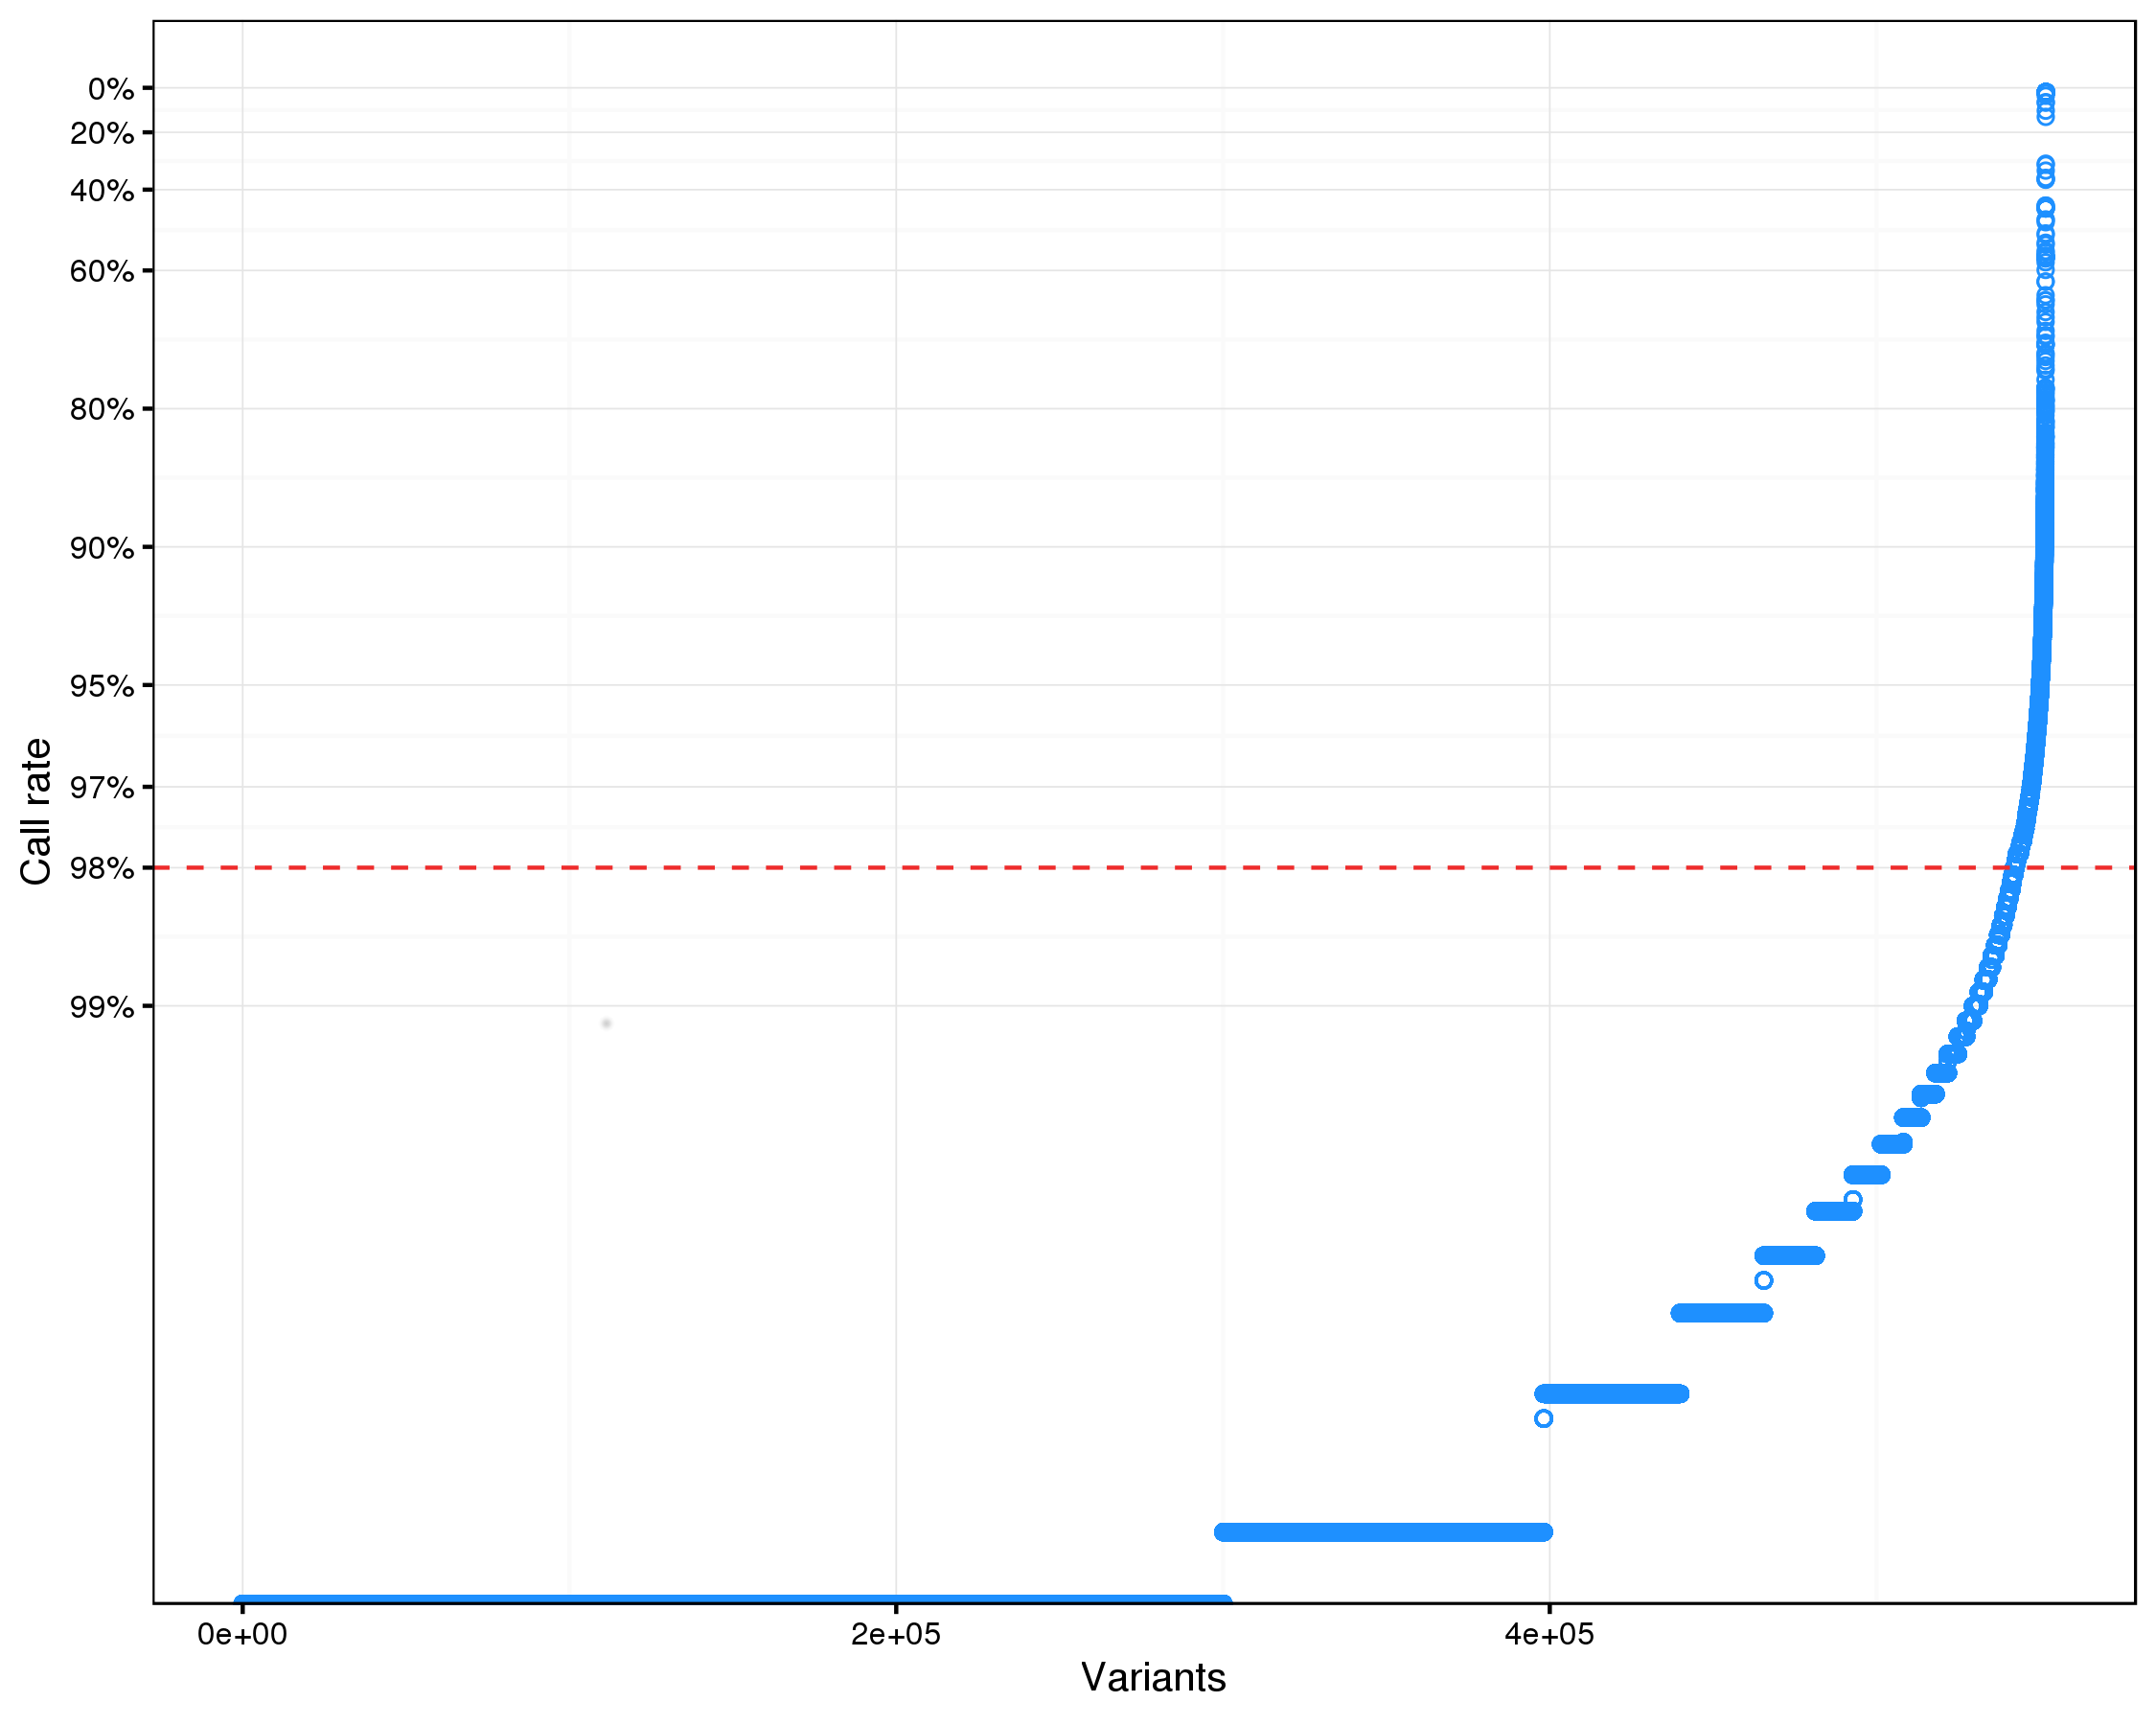
\includegraphics[width=3in,height=2.4in]{FiguresTables/variantbasedQC} 

}

\caption{Taux de génotypage par variant. La ligne rouge
indique le seuil de 98~\%.}\label{fig:variantbasedQC}
\end{figure}

\begin{itemize}
\tightlist
\item
  \emph{Taux de génotypage ou taux de génotypes manquants} (Figure
  \ref{fig:variantbasedQC})\\
  Sur le même principe que le taux de génotypage pour un individu, le
  taux de génotypage d'un SNP est examiné. Un taux de succès,
  généralement fixé à 95~\%, est toléré, seuil en dessous duquel le SNP
  sera exclus des analyses.
\end{itemize}





\begin{figure}[!htb]

{\centering 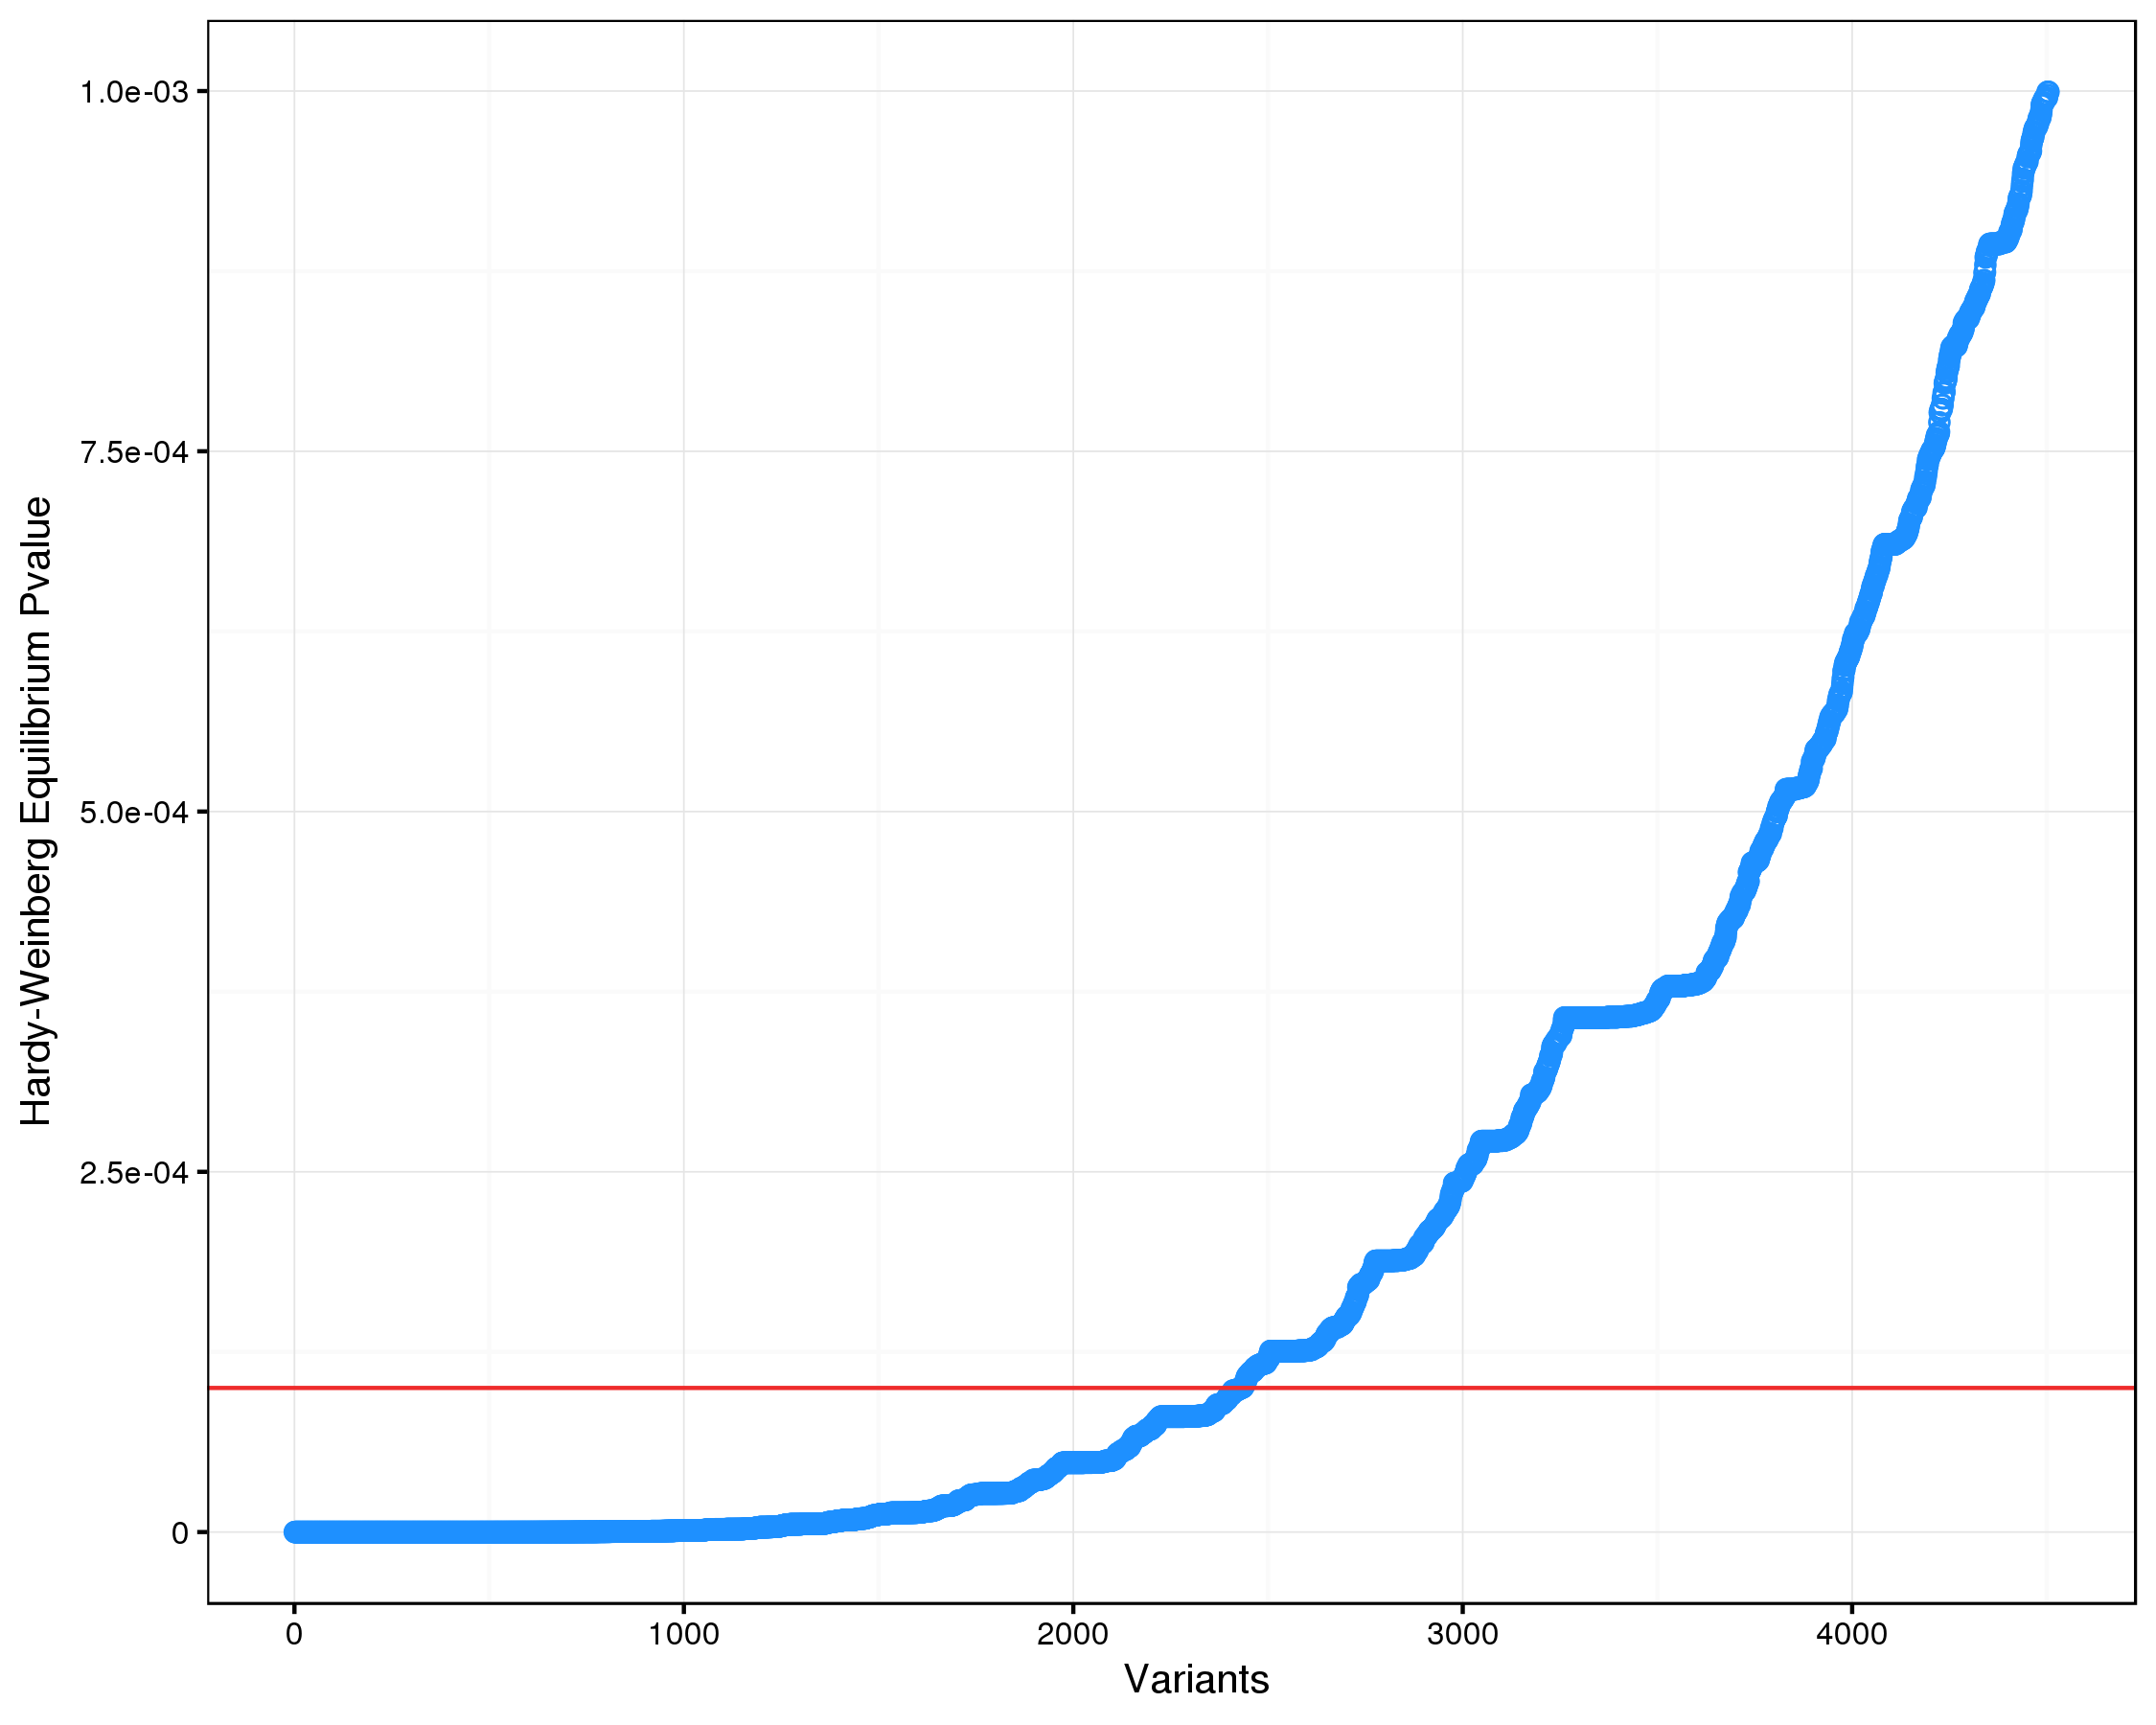
\includegraphics[width=3in,height=2.4in]{FiguresTables/hardyweinbergpvalues} 

}

\caption{Distribution des valeurs-p du test des
variants à l'équilibre de Hardy-Weinberg (HWE). La ligne rouge
horizontale indique le seuil de significativité pour \(\alpha=0,0001\).}\label{fig:hardyweinbergpvalues}
\end{figure}

\begin{itemize}
\tightlist
\item
  \emph{Équilibre de Hardy-Weinberg} (Figure
  \ref{fig:hardyweinbergpvalues})\\
  L'équilibre de Hardy-Weinberg (HWE) constitue l'un des principes
  fondamentaux de la génétique des populations. Pour une population
  suffisamment grande, non apparentée (c.-à-d. population panmictique où
  les accouplements se font au hasard ou de façon équiprobable), sans
  pression de sélection, et lorsque les générations d'individus
  successives sont discrètes et séparées, cet équilibre prédit que les
  proportions génotypiques d'un variant donné restent constantes d'une
  génération à la suivante et s'écrivent simplement comme le produit
  mathématique des fréquences alléliques de cette population. Une forte
  déviation par rapport à l'HWE est un motif d'exclusion d'un SNP dans
  les études associations pangénomiques, car peu probable et sans doute
  révélatrice d'une erreur de génotypage. Mais un écart important par
  rapport à l'HWE peut également indiquer un effet de sélection,
  c'est-à-dire que les cas (dans une étude cas/témoin) peuvent montrer
  une déviation à l'HWE pour des loci associés à la maladie étudiée~:
  exclure ces loci reviendrait donc à exclure ce qui est précisément
  l'objet de l'étude \citep{wittke-thompson_rational_2005}. Ceci
  explique pourquoi le seuil de significativité du test d'écart à l'HWE
  varie d'une étude à l'autre, bien que ce test ne soit effectué que
  dans le groupe témoin
  \citep{meyre_genome-wide_2009, sladek_genome-wide_2007, burton_genome-wide_2007}.
\end{itemize}




\begin{figure}[!htb]

{\centering 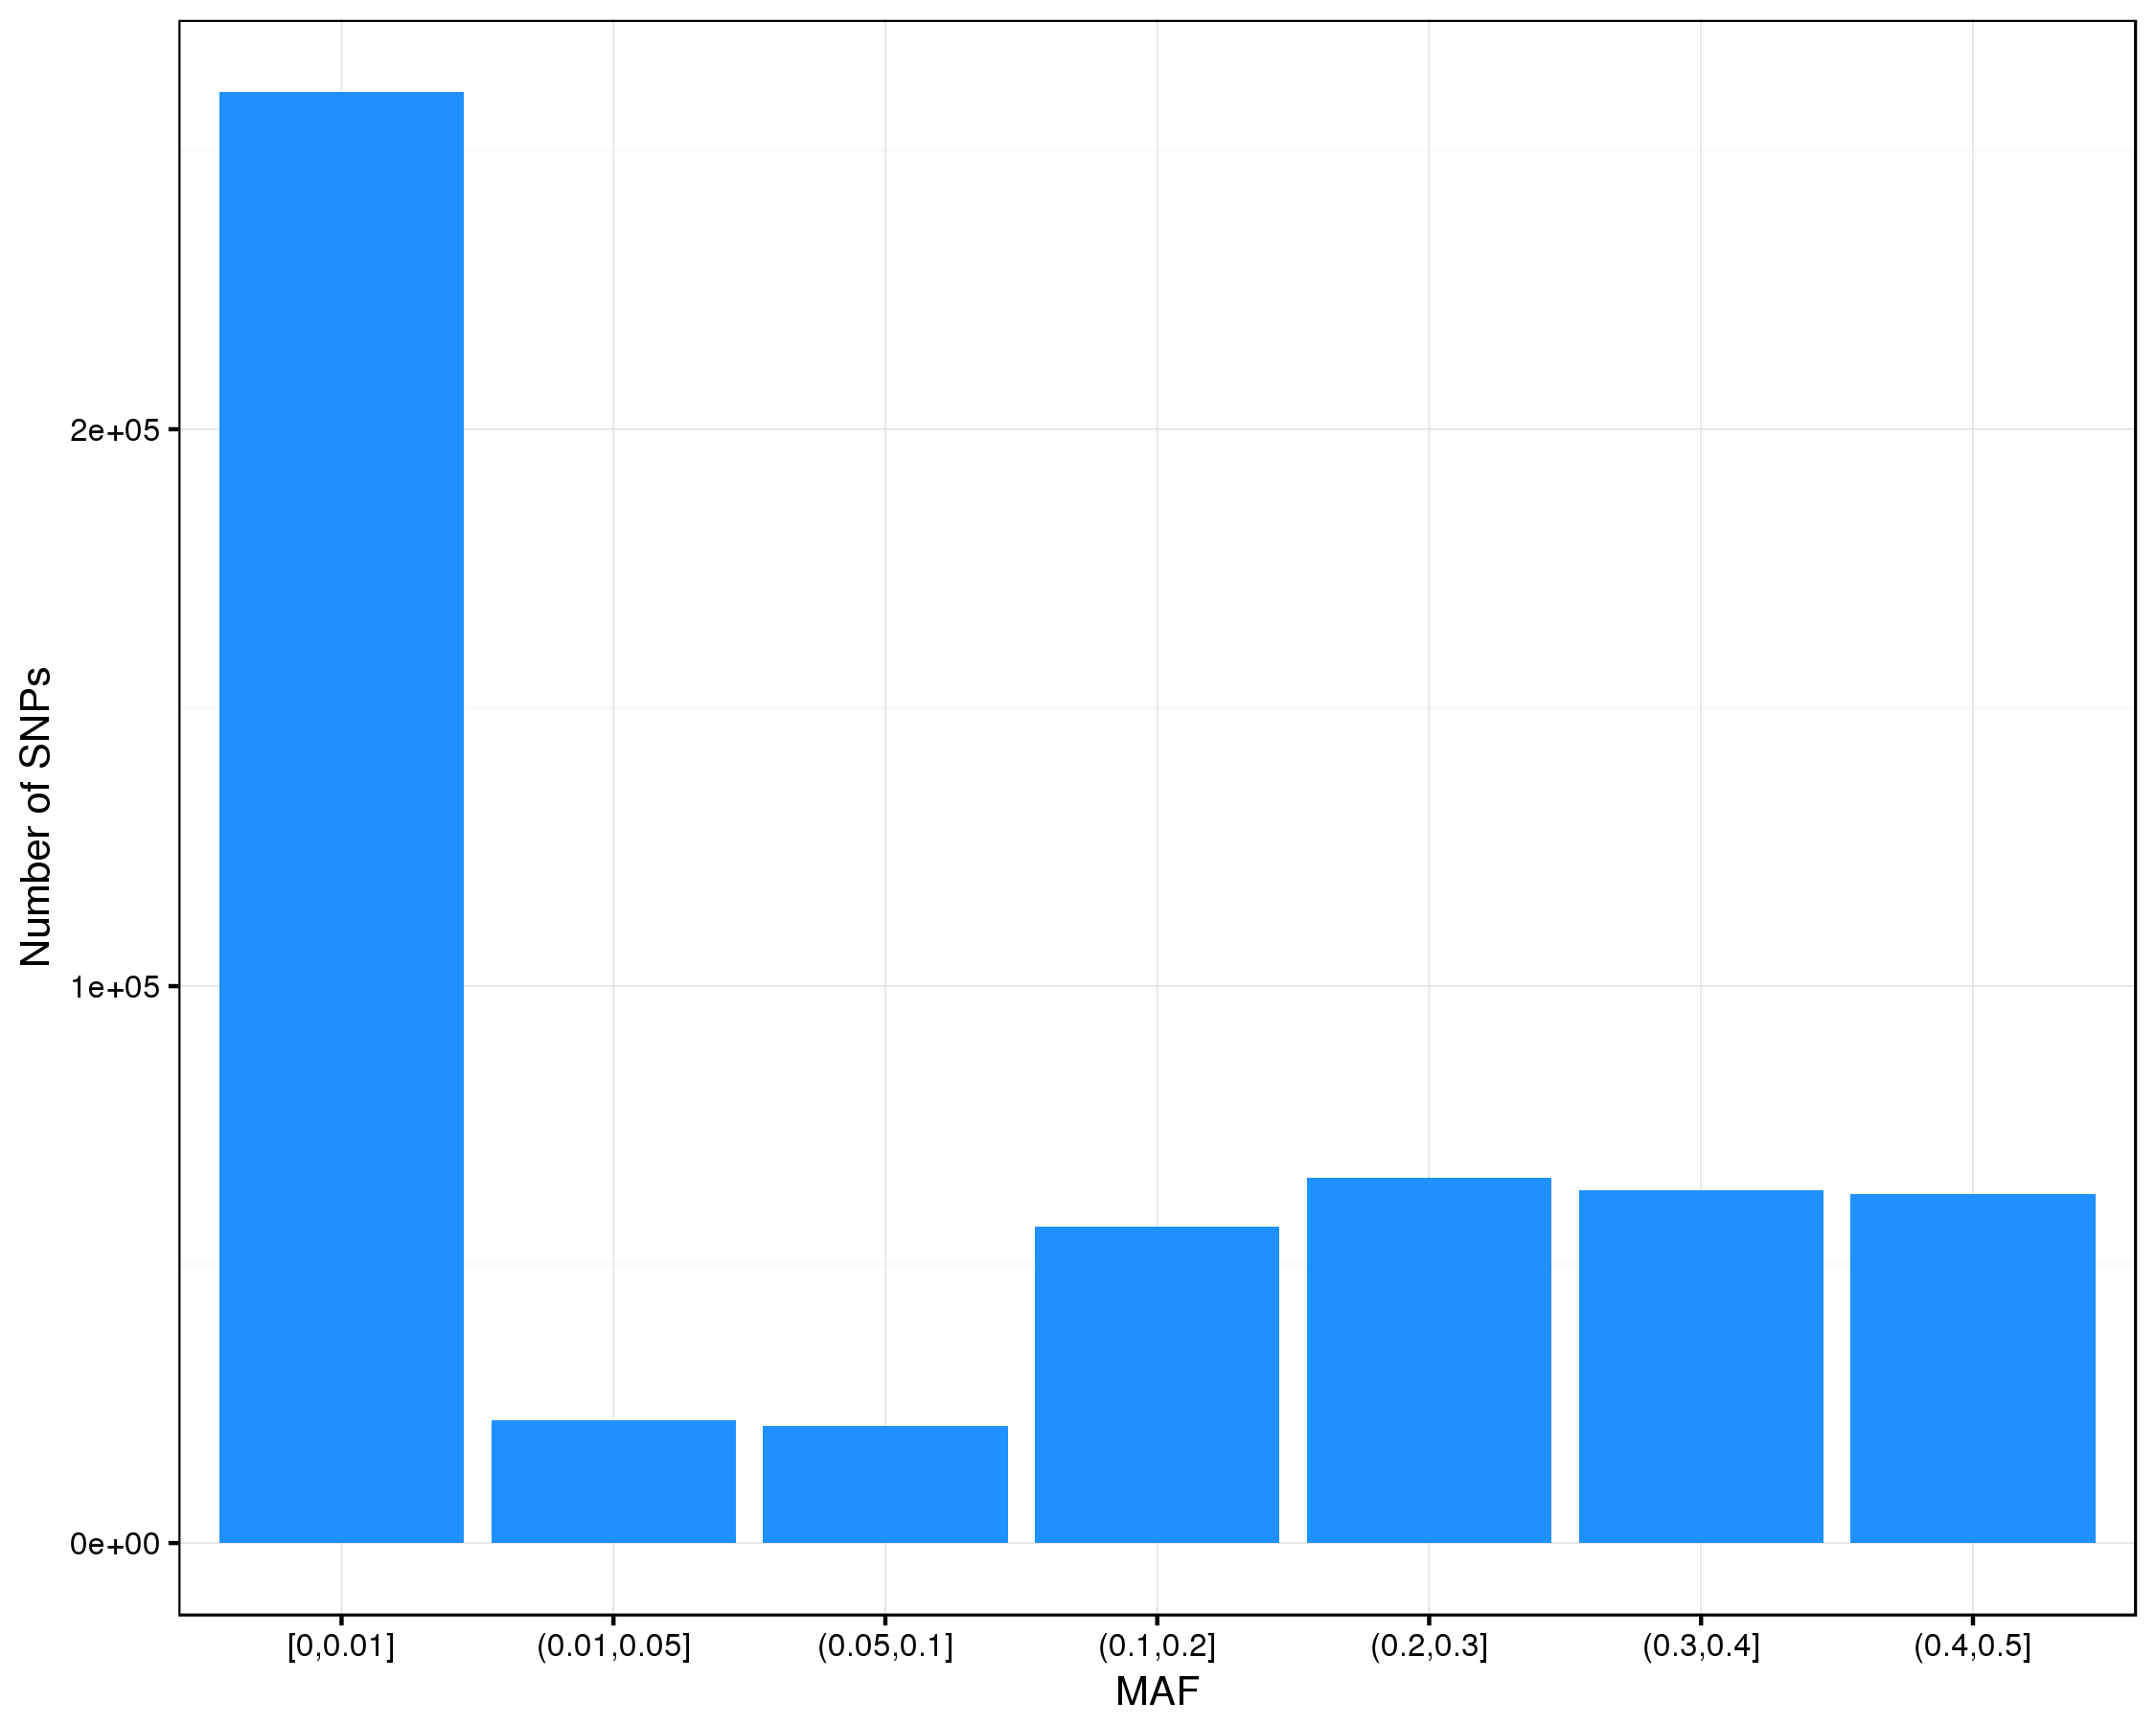
\includegraphics[width=3in,height=2.4in]{FiguresTables/mafdistribution} 

}

\caption{Répartition du nombre de SNP par classe de
fréquence des allèles mineurs (MAF).}\label{fig:mafdistribution}
\end{figure}

\begin{itemize}
\tightlist
\item
  \emph{Fréquence allélique mineure (en anglais, maf)} (Figure
  \ref{fig:mafdistribution})\\
  Un filtre sur la fréquence allélique est appliqué pour ne conserver
  dans les analyses statistiques que les polymorphismes dont la
  fréquence de l'allèle mineur est supérieure à 5~\% (par définition,
  cette fréquence est comprise entre 0 et 50~\%). Dans certaines études,
  pour conserver des SNPs considérés comme ``rares'', c.-à-d. dont la
  maf estinférieure à 5~\%, il est possible d'augmenter le seuil du taux
  de génotypage par SNP \citep{burton_genome-wide_2007}. Cependant, les
  résultats des tests d'associations observés pour ces SNPs rares sont
  moins robustes, malgré un taux de génotypage plus élevé (p.~ex.
  99~\%), principalement parce que ces résultats peuvent être produits
  par les génotypes rares de quelques individus seulement. En effet,
  \citet{morris_evaluation_2010} ont montré que la puissance statistique
  pour détecter des associations pour des SNPs rares était faible,
  particulièrement avec des approches dites ``\emph{simple SNP}'',
  c.-à-d. un SNP à la fois. En réalité, leur exclusion n'aurait qu'un
  impact modéré sur les résultats de l'étude.
\end{itemize}

En conclusion, même après avoir appliqué ces différents filtres de
contrôle-qualité, aussi bien au niveau des individus qu'au niveau des
SNPs, des erreurs de génotypage peuvent subsister, d'où la nécessité de
répliquer les associations détectées dans d'autres échantillons.

\clearpage

\paragraph{Transcriptomique}\label{transcriptomiquePT}

Les données de transcriptomique provenant de la lecture et de la
quantification de la fluorescence d'une puce à ADN nécessitent également
un prétraitement afin de garantir la validité et la fiabilité de
celles-ci. Avant la réalisation d'une étude transcriptomique, une
considération particulière doit être prise quant à la conception du plan
d'expérience pour réduire les biais techniques, p.~ex. en équilibrant
les échantillons sur les puces et plaques, en réalisant l'expérience en
un minimum de temps, ou en limitant le nombre d'expérimentateurs
\citep{quackenbush_microarray_2002}), et ainsi permettre un
contrôle-qualité plus efficace, particulièrement lors de la
normalisation des données.

Les plateformes qui permettent de quantifier l'expression des gènes via
la quantification d'ADN complémentaire (cDNA) à partir de séquences
d'ARN (mRNA, microRNA) ne font pas appel aux mêmes techniques. Plusieurs
outils ont été développés permettant l'importation et le prétraitement
des données brutes directement depuis le logiciel statistique R
\citep{R-limma, R-AgiMicroRna}.

\begin{itemize}
\item
  \emph{Valeur-p de détection}\\
  Selon la plateforme utilisée (principalement chez Illumina), la mesure
  brute d'expression peut être accompagnée d'une valeur-p de détection
  calculée à partir de la mesure d'intensité de sondes contrôles,
  permettant d'évaluer si le signal observé est statistiquement
  différent de l'intensité (artéfactuelle) observée au niveau des sondes
  contrôles. Cette mesure peut alors être utilisée en tant que filtre en
  amont des étapes de normalisation pour exclure les sondes
  non-détectées (à partir d'un seuil, p.~ex. \(\textrm{valeur-p}<0,05\))
  sur un nombre suffisant déterminé par l'expérimentateur ou analyste
  (p.~ex. sonde détectée sur 95~\% des échantillons).
\item
  \emph{Correction du ``bruit de fond''}\\
  En effet, après que les puces à ADN aient été scannées pour évaluer la
  fluorescence des sondes permettant la quantification indirecte de
  l'ARN, deux types de mesures sont disponibles~: l'intensité de
  fluorescence au niveau d'un puits (une sonde par puits) et l'intensité
  de fluorescence ambiante (au voisinage des puits). Cette seconde
  information, appelée ``bruit de fond'', doit être prise en compte.
  Plusieurs approches sont disponibles pour réaliser cette correction de
  l'intensité des sondes (signal) par l'intensité ambiante, dont
  l'approche la plus classique consiste à soustraire l'intensité
  ambiante au signal. Cependant, cette correction produit des effets
  indésirables, puisqu'elle peut générer des valeurs négatives lorsque
  l'intensité ambiante est plus forte que le signal ce qui, lors du
  passage au logarithme ou logarithme-ratios, aboutissent à la
  génération de données manquantes, rendant de ce fait inexploitable ces
  mesures. L'extension R \emph{limma} \citep{R-limma} propose plusieurs
  méthodes pour cette correction du ``bruit de fond'', dont une approche
  basée sur un modèle de convolution normale + exponentielle. Le modèle
  suppose que les intensités observées sont la somme de l'intensité
  ambiante et du signal, l'intensité ambiante suivant une distribution
  normale lorsque le signal suit une distribution exponentielle
  \citep{irizarry_exploration_2003, silver_microarray_2009, ritchie_comparison_2007}.
  Cette méthode permet de garantir que le signal de l'ensemble des
  sondes est strictement positif, et ainsi permet le passage au
  logarithme sans perte de données.
\end{itemize}




\begin{figure}[!htb]

{\centering 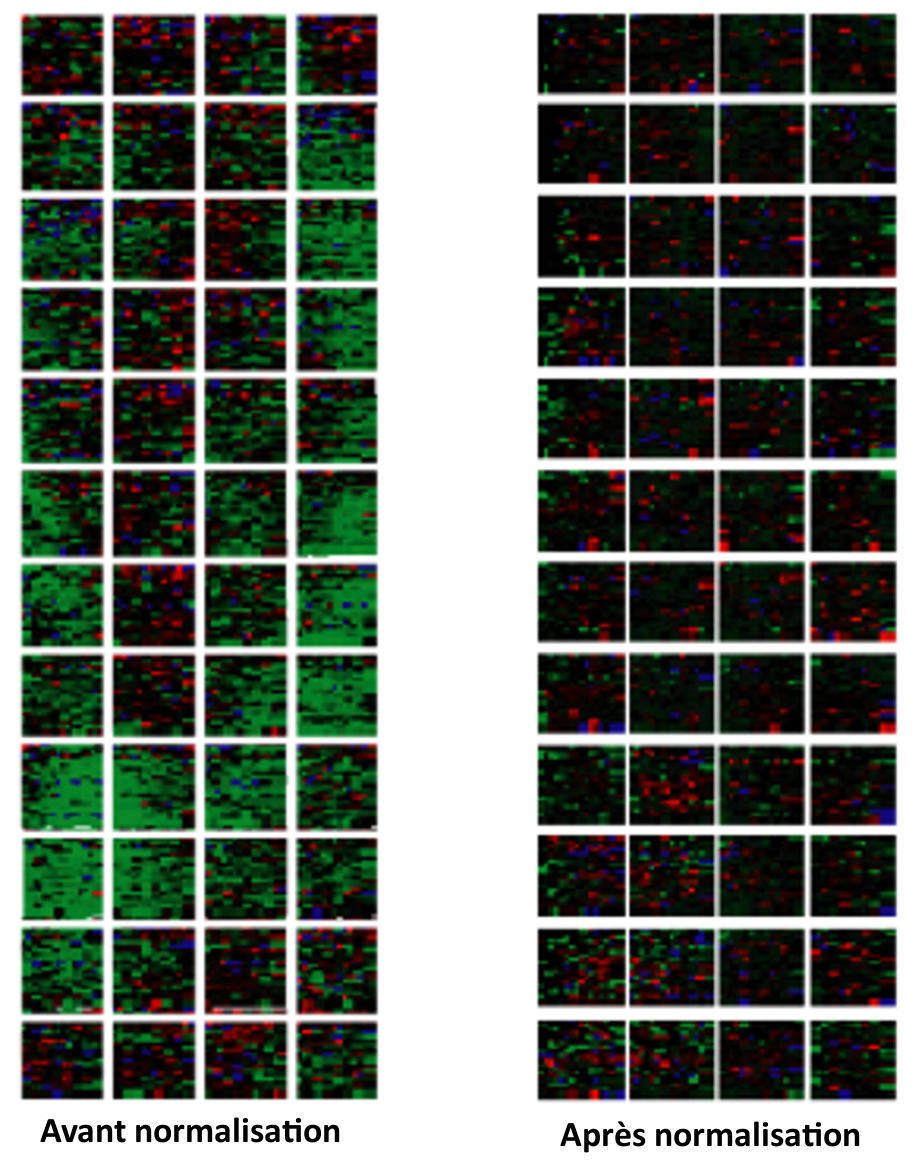
\includegraphics[width=4in,height=3.25in]{FiguresTables/normalisation} 

}

\caption{Données d'expression avant et après normalisation
des intensités.}\label{fig:normalisation}
\end{figure}

\begin{itemize}
\item
  \emph{Normalisation inter-puces}\\
  Une étape de normalisation est réalisée afin de repérer et corriger un
  effet, ou biais, systématique sur l'ensemble des mesures d'expression
  pouvant correspondre à un effet puce, c'est-à-dire qu'il peut exister
  une différence dans l'application des protocoles d'une puce à l'autre
  induisant des mesures systématiquement plus élevées sur une puce en
  particulier. Ces différences techniques peuvent être le résultat d'une
  mauvaise hybridation des cDNA sur une puce, ou d'une faible quantité
  de cDNA aboutissant à des pics de fluorescence plus faibles dans ces
  cas-là (Figure \ref{fig:normalisation}). La principale méthode de
  normalisation utilisée dans les études transcriptomiques est la
  normalisation quantile, permettant de rendre similaire, d'un point de
  vue statistique, deux ou plusieurs distributions. Autrement dit, la
  distribution des mesures d'expression d'une puce est prise en
  référence, et la distribution des mesures obtenues sur une seconde
  puce est normalisée pour que celle-ci soit comparable à la première.
  Dans le même temps, la normalité des mesures d'expression n'étant pas
  toujours vérifiée, une transformation logarithmique (base 2) est
  préalablement appliquée sur les données brutes, ou sur les ratios des
  mesures obtenues~: pour une sonde dans une condition donnée, sa mesure
  est divisée par la mesure obtenue pour la même sonde dans une
  condition contrôle, comme cela est fait dans les expériences de
  quantification par RT-PCR, permettant ainsi la quantification
  (fluorescence) d'un mRNA spécifique via la transcription inverse
  suivie d'une amplification des fragments de cDNA.
\item
  \emph{Filtre des sondes}\\
  Une fois les données normalisées, une étape additionnelle peut être
  appliquée pour filtrer les sondes, par exemple, pour ne conserver que
  les sondes exprimées (à partir d'un seuil défini au préalable, selon
  un gène de ménage servant de référence, c'est-à-dire un gène dont le
  niveau d'expression est constant dans l'ensemble des tissus) sur un
  certain nombre d'échantillons d'une condition (p.~ex. 95~\% des
  individus contrôles).
\item
  \emph{Profil extrême global} (Figure \ref{fig:pcaexpr})\\
  Enfin, un dernier contrôle consiste à la vérification et à
  l'identification d'individus présentant un profil transcriptomique
  extrême, par exemple, au moyen d'une ACP. D'une part, l'ACP permettra
  de pouvoir identifier une éventuelle stratification, au sein des
  individus, associée ou non aux conditions expérimentales~; d'autre
  part, elle permettra d'identifier des individus extrêmes par rapport à
  l'ensemble des conditions ou d'une condition expérimentale donnée, qui
  pourrait être liée à la quantité de cDNA ou à la qualité d'ARN.
\end{itemize}




\begin{figure}[!htb]

{\centering 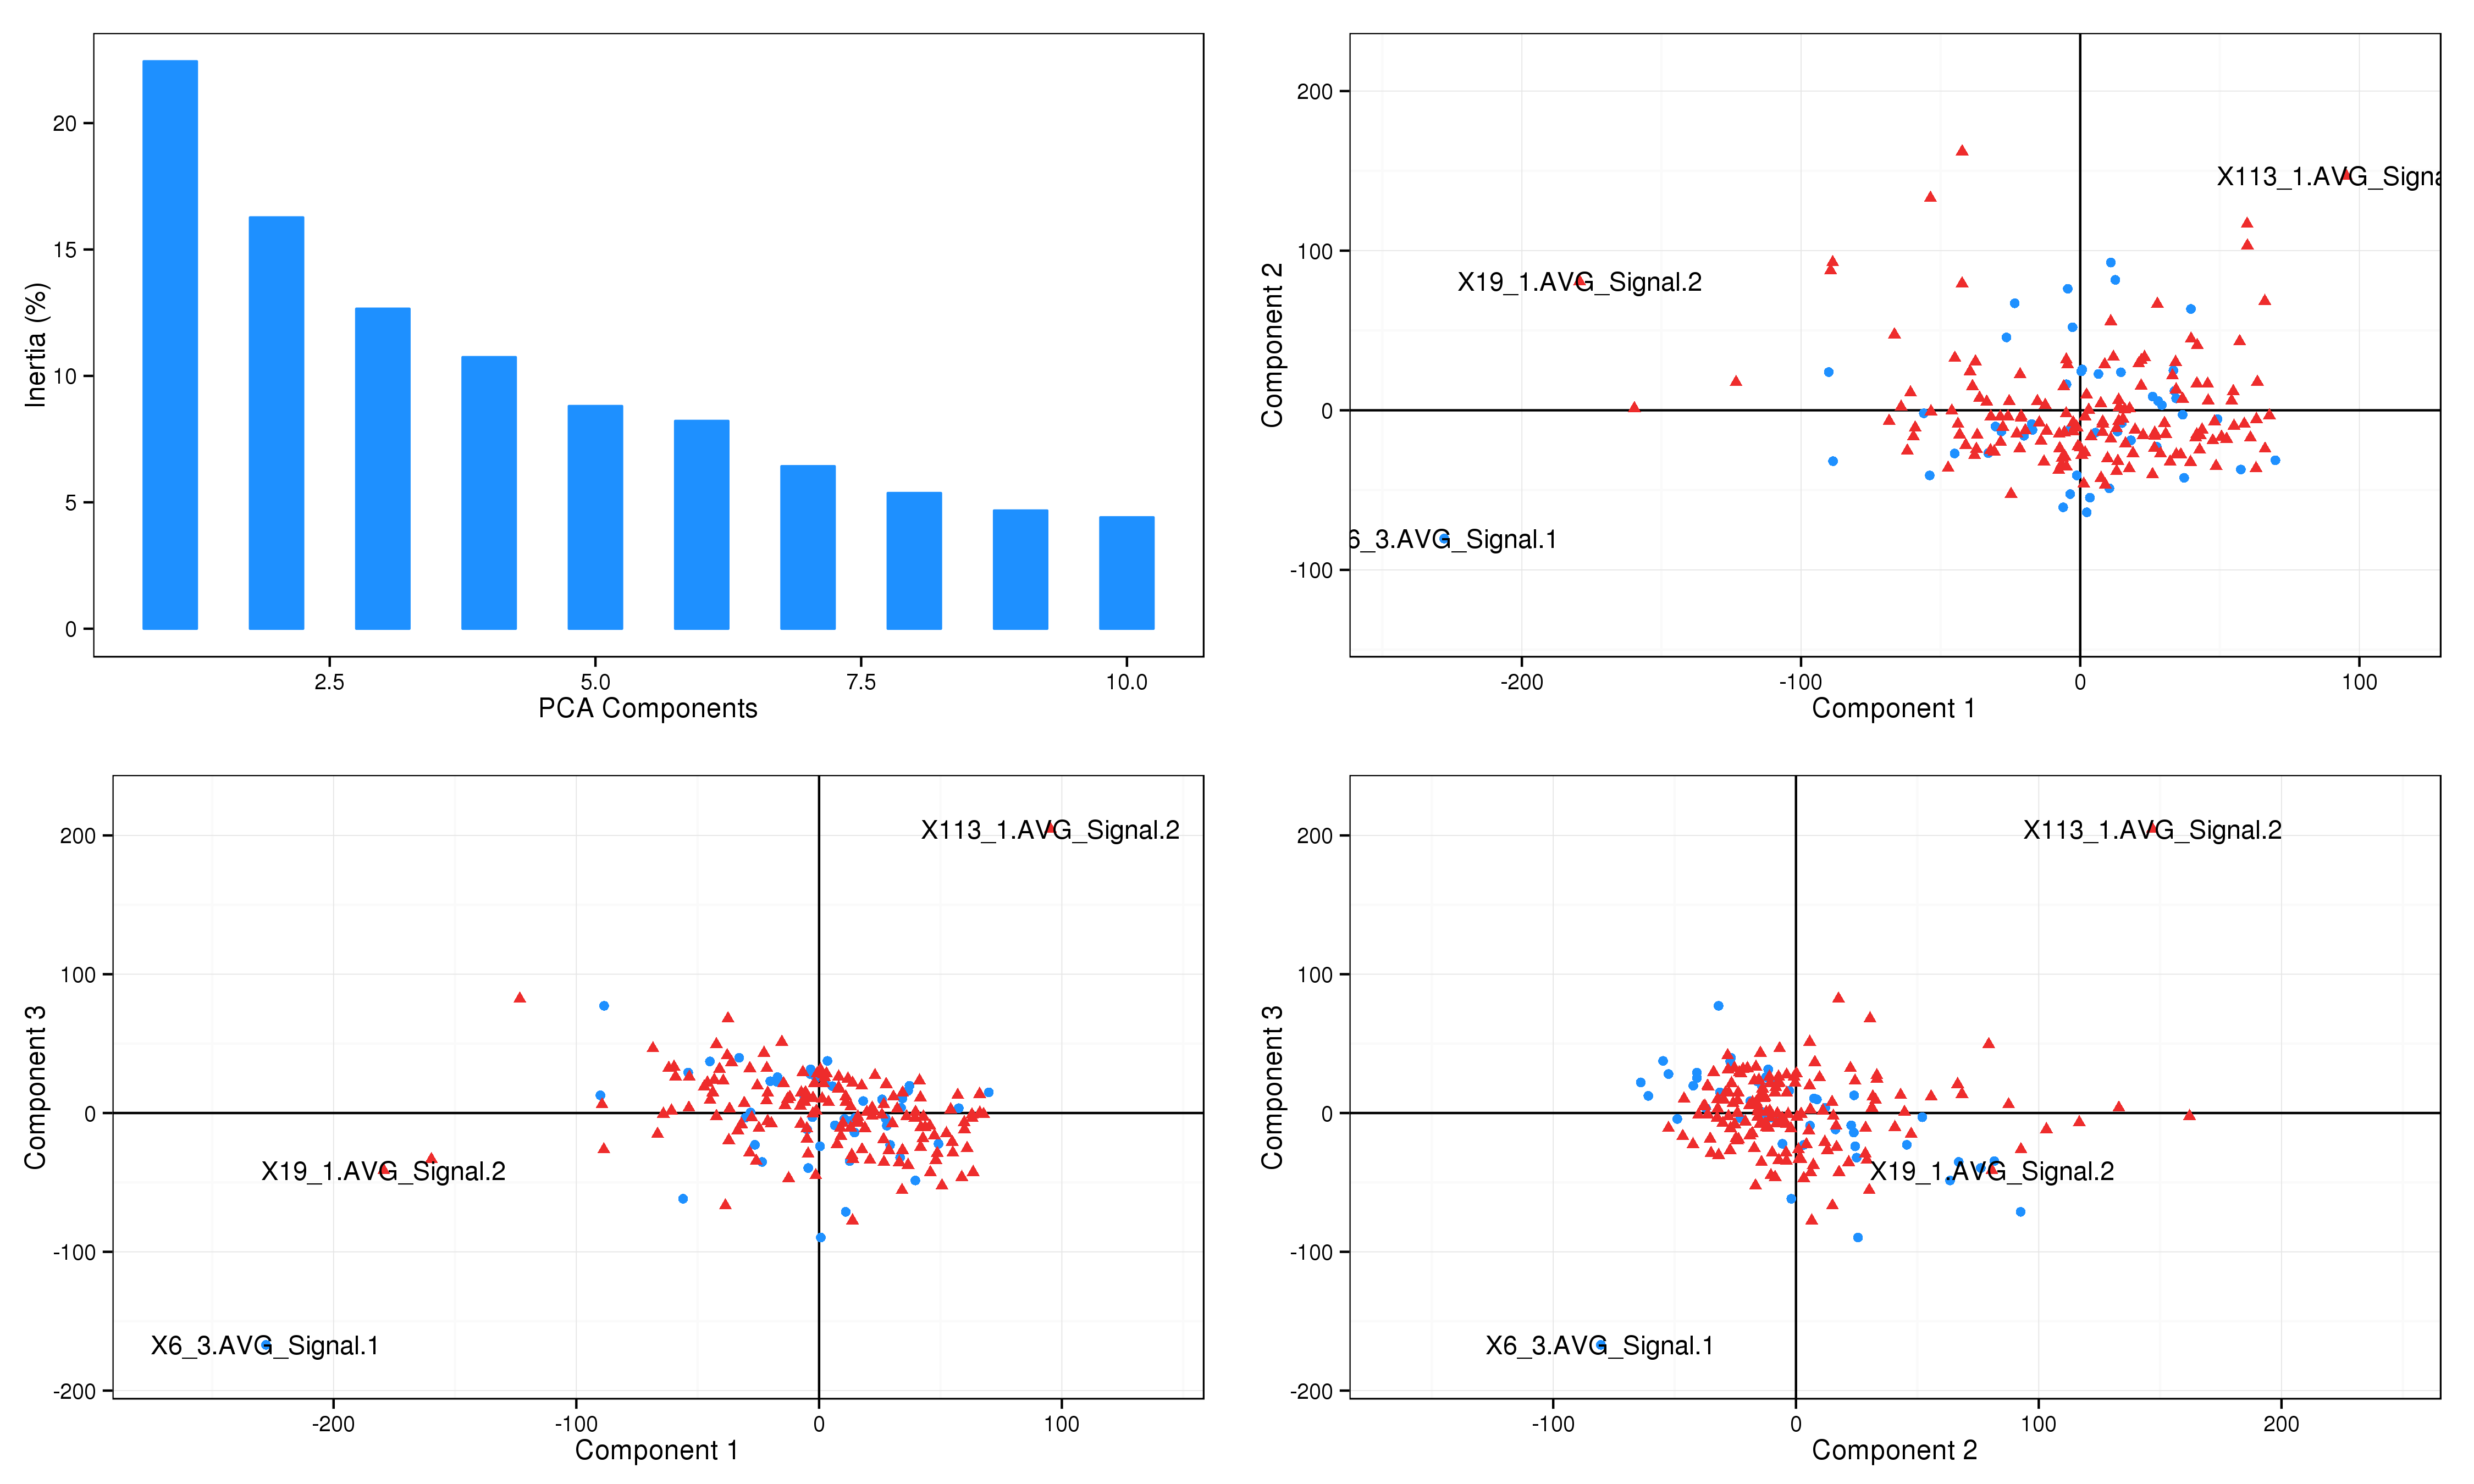
\includegraphics[width=6in]{FiguresTables/pcaexpr} 

}

\caption{Identification de profil extrême à partir des premières
composantes de l'analyse en composante principale.}\label{fig:pcaexpr}
\end{figure}

Les puces à ADN utilisées en transcriptomique n'exploitent pas toutes
les mêmes techniques expérimentales (p.~ex. puce monochrome ou
bi-couleur), nécessitant de ce fait d'adapter les étapes de
prétraitement et de contrôle-qualité décrites précédemment.

\clearpage

\paragraph{Méthylomique}\label{methylomiquePT}

Comme les précédentes techniques omiques, les données de méthylomique
doivent faire l'objet d'un prétraitement et d'un contrôle-qualité. Les
principes et techniques évoqués pour la génomique et la transcriptomique
peuvent et sont employés également en méthylomique. Néanmoins, d'autres
vérifications et certaines adaptations méthodologiques sont nécessaires.
En génomique, les valeurs sont discrètes et codées 0, 1, 2 (modèle
additif)~; en transcriptomique, les valeurs (brutes) sont continues et
définies sur l'intervalle \([0, +\infty(\), tandis qu'en méthylomique,
les données sont bornées entre 0 et 1.


















\begin{figure}[!htb]

{\centering \includegraphics[width=6in]{FiguresTables/Illumina450k} 

}

\caption{Représentation des techniques de marquage utilisées
sur la puce Illumina Infinium HumanMethylation450
\citep{maksimovic_swan:_2012}. a) Infinium I. Chaque CpG est interrogé à
l'aide de deux types de sondes~: méthylée (M) et non-méthylée (U). Les
deux types de sondes incorporent le même nucléotide marqué pour un site
CpG donné, produisant ainsi la même fluorescence. Le nucléotide qui est
ajouté est déterminé par la base en aval du ``C'' du CpG ciblé. Le
pourcentage de méthylation peut être calculé en comparant les intensités
des deux sondes (U et M) de la même couleur. b) Infinium II. Chaque CpG
est interrogé à l'aide d'un seul type de sonde. L'état de méthylation
est détecté par la base complémentaire unique à la position du ``C'' du
CpG ciblé, ce qui entraîne l'ajout d'un nucléotide marqué ``G'' ou
``A'', complémentaire à la cytosine (méthylé) ou à la thymine
(non-méthylé), respectivement. Le pourcentage de méthylation du site CpG
ciblé est déterminé en comparant les intensités des deux couleurs émises
par les nucléotides marqués.}\label{fig:Illumina450k}
\end{figure}

Les étapes décrites ci-après, quoique non-exclusives ou exhaustives,
concernent principalement la puce Illumina HumanMethylation450
\citep{bibikova_high_2011}, puce qui a été utilisée dans l'article du
Chapitre \ref{Article3}. La puce Illumina HumanMethylation450 permet
l'identification de la méthylation sur plus de 450~000 sites CpG
localisés sur l'ensemble du génome, et se caractérise par l'utilisation
de deux processus d'analyses chimiques différents (Infinium I et II).
L'Infinium I utilise un système de marquage fluorescent monocouleur,
tandis que l'Infinium II exploite un système bi-couleur pour quantifier
la méthylation. À cela, s'ajoute un second niveau de différences,
puisque l'Infinium I dispose de deux types de sondes pour identifier les
allèles méthylés et les allèles non-méthylés. L'Infinium II n'utilise
qu'un seul type de sonde qui, lors de l'hybridation des fragments d'ADN
sur la puce, rend accessible ou non la base nucléotidique complémentaire
à celles marquées (T et G pour les sites CpG respectivement non-méthylés
et méthylés) (Figure \ref{fig:Illumina450k}).
\citet{dedeurwaerder_evaluation_2011} ont montré que ces différentes
techniques (c.-à-d. réactions chimiques et types de sonde) impactaient
directement les résultats obtenus. Les extensions R et les algorithmes
de prétraitement des données de méthylation se sont fortement développés
et multipliés ces dernières années, imposant à l'utilisateur la délicate
tâche de sélectionner les méthodes les plus efficaces et les plus
adaptées à ces données.

\subparagraph{Contrôle-qualité des sites
CpG}\label{controle-qualite-des-sites-cpg}

\begin{itemize}
\item
  \emph{Filtre des sites}\\
  En amont, un premier filtre est réalisé pour exclure les sites de
  méthylation pouvant présenter des résultats étranges, principalement
  pour des raisons techniques~:

  \begin{itemize}
  \item
    Sondes trans-réactives\\
    La transformation des cytosines non-méthylées en thymine lors de la
    bisulfitation entraîne un changement dans la distribution des quatre
    bases nucléotidiques dans le génome, et par conséquent augmente la
    probabilité que les sondes Infinium puissent s'hybrider sur d'autres
    portions du génome que celles ciblées initialement. La méthylation
    observée sur ces sites peut donc être le résultat d'un mélange de la
    méthylation du site cible et de celle d'autres sites. Des
    annotations des sites supposés ou vérifiés comme non-spécifiques ont
    été générées pour permettre de les identifier et/ou de les exclure
    \citep{price_additional_2013, zhang_analysis_2012, chen_discovery_2013}.
  \item
    Sondes incluant un SNP\\
    Il peut être nécessaire d'exclure les sondes comportant un SNP,
    puisque la quantification de la méthylation est basée sur le
    génotypage (quantitatif) de C/T (après conversion bisulfite)
    \citep{price_additional_2013, chen_discovery_2013}. En effet, des
    polymorphisme C/T peuvent être présents naturellement chez un
    individu, et ainsi être considérés comme un résultat de la
    conversion bisulfite. La séquence d'ADN est alors confondue avec la
    méthylation. Par exemple, un individu homozygote C/C aura une
    méthylation proche de 100~\%, pendant qu'un individu homozygote T/T
    aura quant à lui une méthylation de 0~\%. Enfin, un individu
    hétérozygote C/T sera à 50~\% méthylé sur ce site. En l'absence de
    données de génomique conjointement aux données de méthylomique, il
    est préférable d'exclure ces sondes et les sites correspondants
    avant analyse.
  \item
    Valeur-p de détection\\
    Tout comme pour les puces d'expression d'Illumina, les puces de
    méthylation fournissent, en plus de la quantification de la
    méthylation, des valeurs-p de détection pour l'ensemble des
    sondes/sites basées sur des sondes contrôles. Par exemple, dans
    l'étude présentée au Chapitre \ref{Article3}), une méthode dérivée
    du contrôle-qualité appliqué en génomique a été utilisée. Ainsi, un
    site est exclu dès lors que la valeur-p de détection est supérieure
    à \(10^{-6}\) pour au moins 5~\% des échantillons. Un filtre
    équivalent est appliqué sur les échantillons, à savoir qu'un
    échantillon doit présenter des valeurs-p de détection inférieures à
    \(10^{-6}\) pour plus de 75~\% des sites pour être conservé.
  \end{itemize}
\item
  \emph{Normalisation}

  \begin{itemize}
  \item
    Intra-puce~: Infinium I/II\\
    Une première normalisation est nécessaire pour corriger les
    différences de distribution des niveaux de méthylation entre
    Infinium I et Infinium II. Cette étape de normalisation Infinium
    I/II est indispensable~; cependant, il convient de choisir la bonne
    méthode après avoir examiné soigneusement la distribution des
    valeurs de méthylation
    \citep{marabita_evaluation_2013, yousefi_considerations_2013}.\\
    Plusieurs méthodes ont été développées~:

    \begin{itemize}
    \item
      ``Peak Based Correction'' (PBC)
      \citep{dedeurwaerder_evaluation_2011}~: la distribution bimodale
      des valeurs de méthylation, avec un pic pour les sites
      non-méthylés et un pic pour les sites méthylés, de l'Infinium I
      est utilisée comme référence pour fixer les deux modes des valeurs
      de méthylation de l'Infinium II.
    \item
      ``Subset quantile Within-Array Normalisation'' (SWAN)
      \citep{maksimovic_swan:_2012}~: une normalisation quantile est
      appliquée à une sélection aléatoire de sondes Infinium I et
      Infinium II (dont la composition en nombre de sites CpG est
      similaire et par type de sondes de l'Infinium II). Les
      distributions (similaires) ainsi obtenues sont ensuite utilisées
      pour ajuster (interpolation linéaire) les valeurs des sondes
      restantes. Similaire à l'approche SWAN, l'approche ``Subset
      Quantile Normalisation'' (SQN) \citep{touleimat_complete_2012} ne
      diffère que par la classification des sondes, effectuée selon leur
      position par rapport aux îlots CpG.
    \item
      ``Beta-Mixture Quantile Normalisation'' (BMIQ)
      \citep{teschendorff_beta-mixture_2013}~: la densité de
      distribution des valeurs de méthylation des Infinium I et II est
      chacune décomposée en un mélange de trois distributions Bêta, où
      chaque distribution Bêta correspond à un état de méthylation~:
      non-méthylé (proche de 0~\%), hémi-méthylé (proche de 50~\%), et
      méthylé (proche de 100~\%). Une normalisation quantile est ensuite
      appliquée entre chaque distribution Bêta de l'Infinium II et la
      distribution Bêta correspondante de l'Infinium I (Figure
      \ref{fig:BMIQ}).
    \end{itemize}
  \item
    Intra-puce~: ``bruit de fond''\\
    Une correction du ``bruit de fond'' suivant les mêmes stratégies que
    celles appliquées pour les puces d'expression (p.~ex. modèle par
    convolution Normale + Exponentielle)
    \citep{xu_enmix:_2015, triche_low-level_2013}.
  \item
    Inter-puce\\
    Une étape supplémentaire de normalisation peut être appliquée pour
    réduire autant que possible les effets ``plaques'' et ``puces''. Des
    méthodes ont été développées dans cet objectif, comme la méthode
    \emph{ComBat} \citep{johnson_adjusting_2007, leek_sva_2012}), ayant
    déjà montré son efficacité sur des données de méthylation
    \citep{sun_batch_2011, leek_tackling_2010}. Cependant, il convient
    de faire attention à l'utilisation de ces méthodes, notamment
    lorsqu'elles permettent d'inclure des informations sur les
    conditions biologiques testées (p.~ex. groupes cas et contrôle)
    \citep{nygaard_methods_2015}. Il est également important de garder à
    l'esprit que la meilleure façon d'éviter les problèmes liés aux
    effets ``plaques'' et ``puces'' est d'avoir réalisé un plan
    d'expérience ex ante, c'est-à-dire d'avoir prévu la répartition des
    échantillons et conditions de façon homogène entre les puces.
  \end{itemize}
\end{itemize}






\begin{figure}[!htb]

{\centering 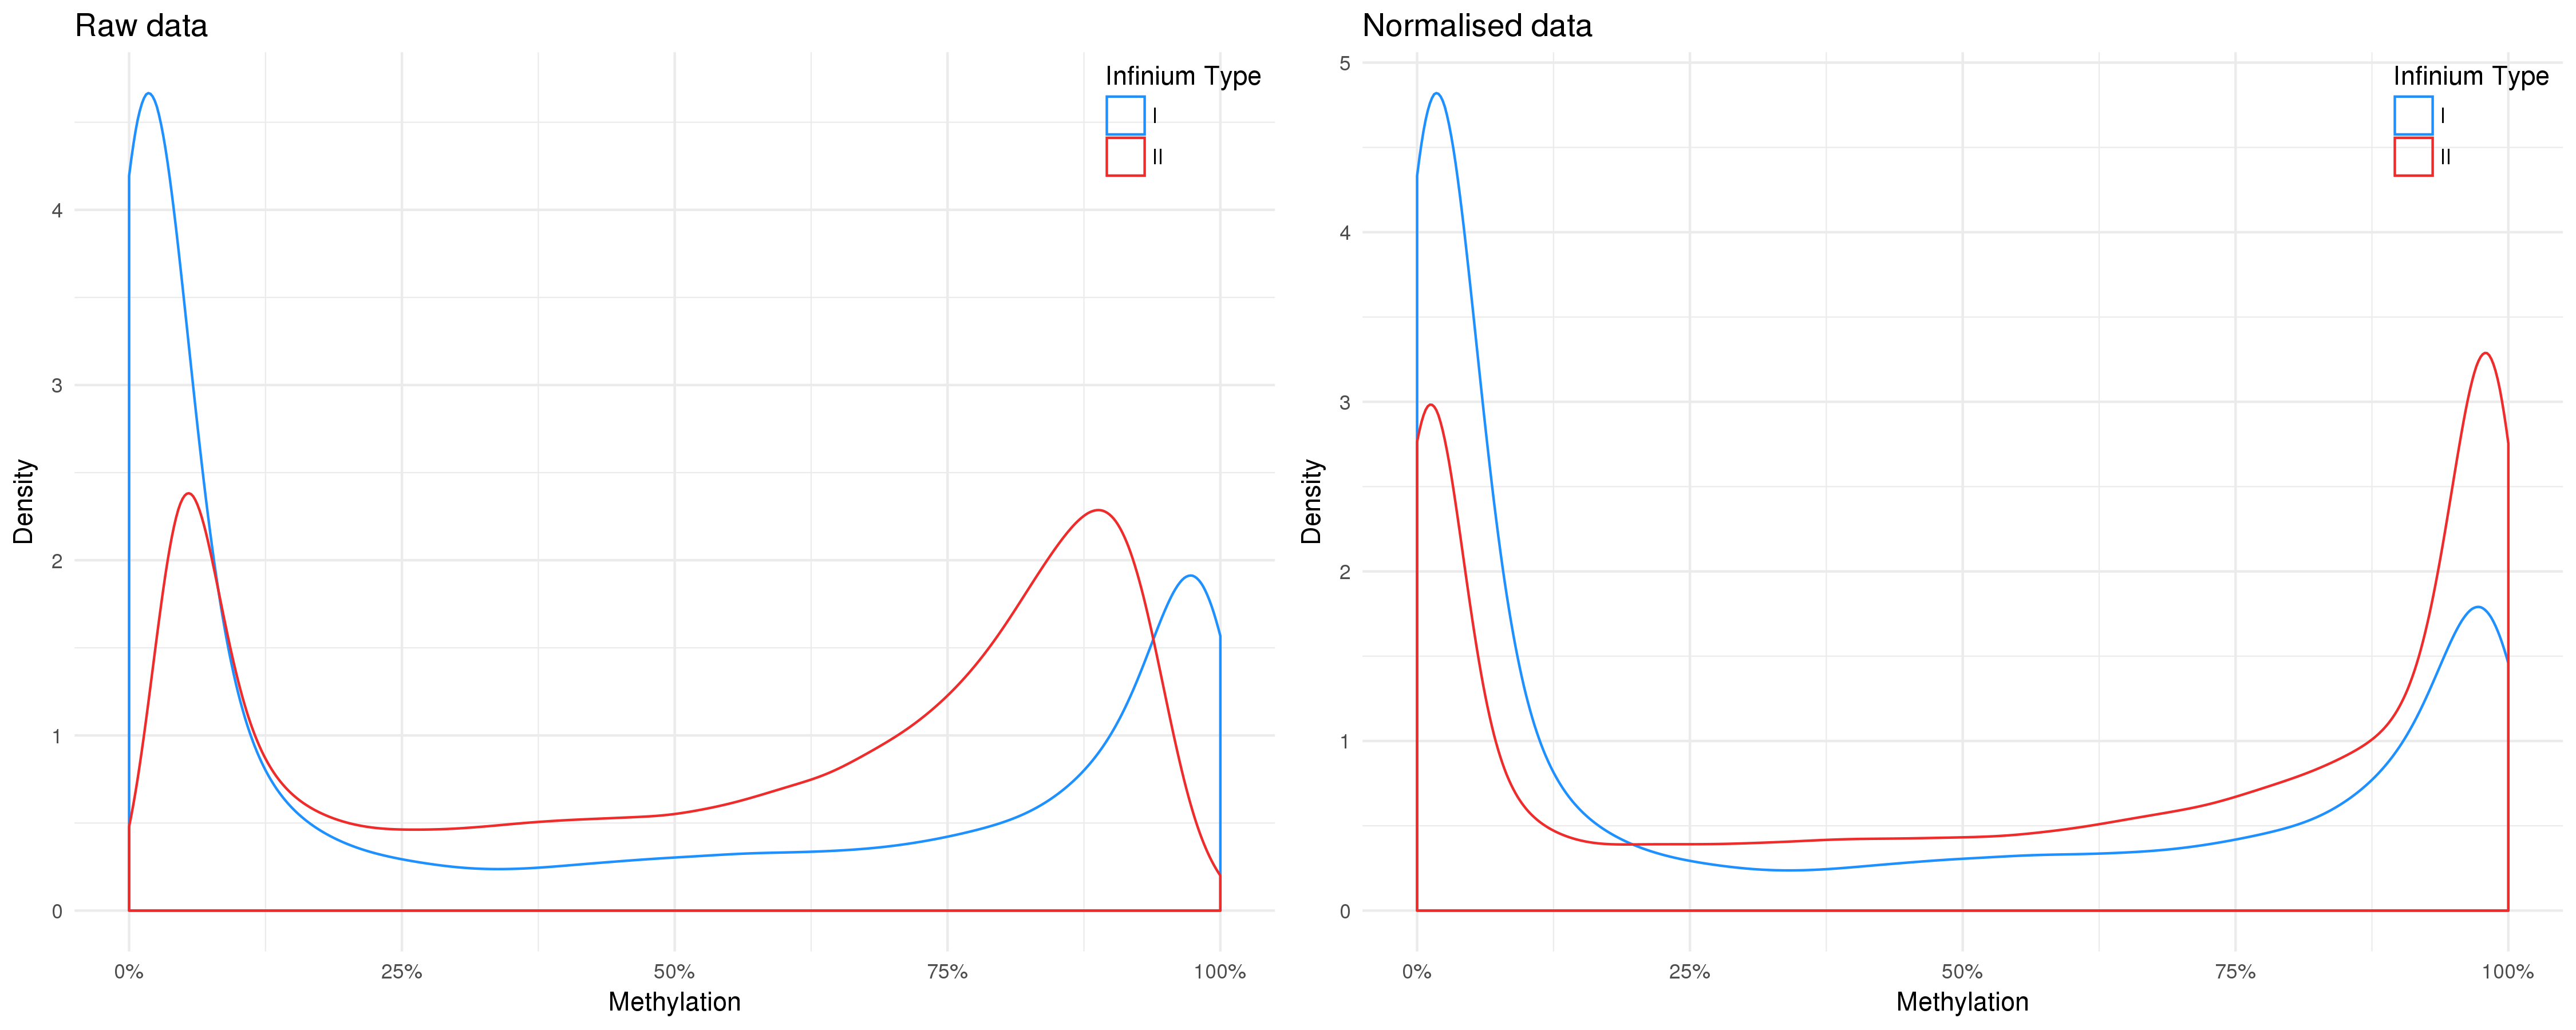
\includegraphics[width=6in,height=2.4in]{FiguresTables/InfiniumType} 

}

\caption{Distribution des valeurs-\(\beta\) de méthylation des sondes
Infinium I et II, avant normalisation BMIQ
\citep{teschendorff_beta-mixture_2013} (à gauche) et après normalisation
BMIQ (à droite).}\label{fig:BMIQ}
\end{figure}

\subparagraph{Contrôle-qualité des
échantillons}\label{controle-qualite-des-echantillons}

Un premier contrôle des échantillons est réalisé lors de l'application
du filtre sur les valeurs-p de détection, permettant ainsi d'exclure les
individus ayant une faible qualité de détection, résultant d'une
dégradation de l'ADN, par exemple. De la même façon qu'en génomique et
transcriptomique, une ACP peut être réalisée dans le but d'identifier
des échantillons dont le profil de méthylation est extrême, et
identifier une stratification des données qui pourrait être liée à un
biais technique non pris en compte.

\subsection{Analyses omique et
multi-omique}\label{analyses-omique-et-multi-omique}

\subsubsection{Génomique}\label{genomique-1}

\paragraph{Avant l'ère des études d'association
pangénomiques}\label{avant-lere-des-etudes-dassociation-pangenomiques}

En l'absence de données omiques, et plus particulièrement de données
génomiques, les études d'\emph{agrégation}, d'\emph{héritabilité} et/ou
de \emph{ségrégation} oont permis de mettre en avant la contribution de
la génétique à de nombreuses pathologies, en se basant sur
l'apparentement d'individus provenant d'une même famille. Ces études
sont réalisées dans un certain ordre, consistant à évaluer en premier
lieu, le caractère héritable d'un trait (binaire ou quantitatif), et en
second lieu, le mode de transmission génétique d'une génération à la
suivante.

\begin{itemize}
\item
  • Les études d'agrégation (pour traits binaires, par exemple, le
  statut diabétique
  \citep{bijanzadeh_recurrence_2017, weijnen_risk_2002}) ont pour but
  d'évaluer le risque relatif d'un trait entre les membres d'une famille
  \citep{laird_15_2000}. Dans ces études, un individu porteur de la
  pathologie est dit ``proband''. Même si ces études permettent de
  montrer qu'un certain trait peut se retrouver de façon plus importante
  dans une famille plutôt que dans une autre (c.-à-d. agrégation), elles
  ne permettent pas d'éliminer un potentiel effet de confusion produit
  par l'environnement, puisque celui-ci peut être identique pour tous
  les individus d'une même famille.
\item
  Les études d'héritabilité (pour traits quantitatifs, par exemple, la
  glycémie à jeun) ressemblent aux études d'agrégation, et cherchent à
  évaluer l'effet de la génétique dans la variabilité d'un trait
  quantitatif. On parle de cet effet comme l'héritabilité d'un trait,
  laquelle donne la proportion de la variabilité totale du trait qui est
  expliquée par l'ensemble des variations liées à la génétique.
\item
  Les études de ségrégation ont pour objectif d'identifier le mode de
  transmission génétique d'un trait, à savoir si le gène de
  susceptibilité suit un modèle génétique de type récessif/dominant,
  additif ou de codominance. Ces différents modes de transmission
  mendélienne s'illustrent bien en utilisant le groupe sanguin ABO
  (phénotype), où les allèles sont définis par A, B et O. L'allèle O est
  l'allèle récessif par rapport aux allèles A et B~: ainsi, un génotype
  A/O donnera le groupe sanguin A, tandis que le génotype B/O donnera le
  groupe sanguin B. Le groupe sanguin AB est issu de la codominance des
  allèles A et B. Enfin, dû au caractère récessif de l'allèle O, un
  individu doit être porteur de deux allèles O (génotype O/O) pour
  présenter un groupe sanguin O.
\end{itemize}

Ces différentes études ont initialement été développées lorsque les
techniques de génotypage étaient onéreuses, et ont servi en quelque
sorte d'études préliminaires aux études d'association pangénomiques.

\paragraph{Les études d'association
pangénomiques}\label{les-etudes-dassociation-pangenomiques}

Les études d'association génétiques se sont développées au cours des 20
dernières années, et viennent compléter les études de liaison qui
quantifie l'excès d'allèles transmis par descendance (selon les
principes mendéliens) entre des individus apparentés (principalement, du
premier et second degré). Nous distinguerons deux types d'études
d'association~: d'une part, lorsque l'analyse porte sur des familles, et
d'autre part, lorsque l'analyse porte sur des individus non apparentés.
Dans le cas des études familiales, en particulier des trios
correspondant à un enfant atteint/porteur et de ses deux parents, le
principal test employé est le test du déséquilibre de transmission
(TDT). Ce test se base sur une statistique calculée par
\((t-u)^2 / (t+u)\), où \(t\) le nombre d'allèles transmis et \(u\) le
nombre d'allèles non transmis. Sous l'hypothèse nulle d'indépendance des
distributions de \(t\) et \(u\), cette statistique suit une distribution
du \(\chi^2\) à 1 degré de liberté. Dans le contexte des études
familiales, ce test confère une puissance statistique plus importante
que les tests d'association classiques avec design cas/témoins, et
limite l'effet lié à une stratification de la population d'étude,
notamment en faisant l'hypothèse d'une homogénéité phénotypique
intra-famille plutôt qu'inter-famille.

\subparagraph{\texorpdfstring{L'approche dite
``classique''}{L'approche dite classique}}\label{lapproche-dite-classique}

Les études d'association pangénomiques (GWAS), dont la toute première a
été réalisée en 2005 \citep{klein_complement_2005}, et la première dans
le diabète de type 2 en 2007 \citep{sladek_genome-wide_2007}, ont été le
principal moteur dans la découverte de nombreux loci de susceptibilité à
diverses maladies complexes, et sont répertoriées au sein de la base de
données ``GWAS Catalog'' \citep{macarthur_new_2017}. Deux raisons
principales expliquent cet essor~: la première est la limite de
détection du TDT dans les maladies complexes (non monogéniques), où
l'excès de transmission de chaque allèle contribuant à cette maladie est
modéré voire faible. La seconde raison concerne les études de puissance
réalisées au début des années 2000
\citep{risch_future_1996, sham_power_2000} qui suggéraient un gain de
puissance statistique pour détecter des associations dans les études
d'association comparativement aux études de liaison. Cependant, ce gain
de puissance demeure relatif, puisque celui-ci dépend de la fréquence
allélique ou encore du déséquilibre de liaison entre les loci étudiés
\citep{tu_power_1999}.

Une étude GWA consiste généralement en l'application d'un modèle de
régression logistique ou linéaire généralisé, selon la nature du trait
étudié, à l'ensemble des polymorphismes identifiés via une puce ADN. Le
nombre de SNPs est passé de près de 300~000 à plusieurs millions, en
particulier grâce à des techniques d'imputation du génome
\citep{howie_genotype_2011} à l'aide de génome de référence
\citep{the_1000_genomes_project_consortium_global_2015}, permettant de
ce fait de pallier aux spécificités des différentes puces, et
d'accroître d'autant la quantité d'information génétique disponible pour
chaque individu.

\begin{equation}g[E(\boldsymbol{Y})]=\beta_0 + \beta_1 \boldsymbol{X} + \beta \boldsymbol{Z}\label{eq:GWAS}\end{equation}

Le modèle classique de régression donné par l'Équation \eqref{eq:GWAS}
consiste à expliquer un trait \(Y\), par exemple le statut DT2 (binaire)
ou la glycémie à jeun (quantitatif), par des SNPs avec en général une
hypothèse d'additivité des allèles. Ainsi le génotype \(X\) est codé 0
pour le génotype homozygote majeur (c.-à-d. homozygote pour l'allèle
avec la plus forte fréquence allélique), 1 pour le génotype hétérozygote
et 2 pour le génotype homozygote mineur (Tableau
\ref{tab:codingGenotype}).\\
La fonction \(g(.)\) est la fonction de lien, par exemple, la fonction
\(logit\) (\(log\left(\frac{P(Y=1)}{1-P(Y=1)}\right)\)) dans le cas où
\(Y\) est dichotomique (régression logistique), ou encore la fonction
\emph{identité} lorsque \(Y\) est quantitatif (régression linéaire).\\
Ces approches sont préférées aux approches basées sur la construction de
table de contingence (p.~ex. test exact de Fisher), en particulier, dans
les études cas/témoins, puisque ces dernières permettent l'ajustement à
des covariables (\(Z\)) cliniques ou démographiques, par exemple. En
outre, l'usage d'un modèle de régression logistique permet de fournir
des odds ratios à partir de la mesure de l'effet \(\beta_1\) du génotype
\(X\).



\begin{longtable}[]{@{}ccccc@{}}
\caption{\label{tab:codingGenotype}Codage du génotype selon le modèle génétique.}\tabularnewline
\toprule
Génotype & Codominant & Additif & Recessif & Dominant\tabularnewline
\midrule
\endfirsthead
\toprule
Génotype & Codominant & Additif & Recessif & Dominant\tabularnewline
\midrule
\endhead
AA & \(X=(01)\) & \(X=2\) & \(X=1\) & \(X=1\)\tabularnewline
Aa & \(X=(10)\) & \(X=1\) & \(X=0\) & \(X=1\)\tabularnewline
aa & \(X=(00)\) & \(X=0\) & \(X=0\) & \(X=0\)\tabularnewline
\bottomrule
\end{longtable}

Des covariables d'ajustements (\(Z\)) sont également ajoutées au modèle,
particulièrement lorsque le plan d'expérience n'a pas permis de prendre
en compte celles-ci. Malgré un plan d'expérience prenant en compte
différents paramètres essentiellement techniques, pouvant être sources
de confusion dans l'analyse, il n'est pas toujours possible de tous les
contrôler dans un même plan d'expérience. Ainsi, ces variables
techniques, démographiques et cliniques peuvent être incluses dans le
modèle en tant que covariable, par exemple, l'âge, le sexe ou encore
l'IMC. D'autres éventuelles variables peuvent être incluses, comme les
premières composantes (deux à cinq) de l'ACP réalisée lors du
contrôle-qualité, permettant de prendre en compte une stratification ou
mélange (p.~ex. ethnique ou géographique) au sein de la population
d'étude
\citep{novembre_genes_2008, clayton_population_2005, bouaziz_accounting_2011}.
L'ajustement pour ces covariables est effectué pour deux raisons
principales~: soit pour éviter de confondre la relation entre le
génotype et le phénotype, soit pour réduire la variance résiduelle et
ainsi augmenter la précision des estimations.

\subparagraph{\texorpdfstring{Les approches
``longitudinales''}{Les approches longitudinales}}\label{les-approches-longitudinales}

Les études GWA classiques se concentrent sur une seule mesure d'un trait
quantitatif par individu pour identifier des variants génétiques, même
lorsque des données longitudinales étaient disponibles, principalement à
cause de la complexité des modèles permettant d'analyser ces données et
en particulier, les temps élevés de calcul. L'utilisation des modèles
linéaires mixtes (LMM)
\citep{laird_random-effects_1982, liang_longitudinal_1986}, des
équations estimantes généralisantes (GEE)
\citep{ziegler_generalised_1998}, et d'autres approches pour prendre en
compte les mesures répétées, est devenue plus fréquente dans les études
GWA, avec notamment des groupes de travail (Genetic Analysis Workshop
18) dont la thématique portait sur les méthodes permettant l'analyse des
données longitudinales dans un contexte génétique
\citep{almasy_data_2014, beyene_longitudinal_2014, wu_mixed-effects_2014}.
Les méthodes LMM et GEE permettent de prendre en compte différentes
structures de données telles que les données longitudinales et
familiales. Cependant, ce type de données comporte habituellement de
nombreuses données manquantes, et nécessite de vérifier certaines
hypothèses quant à leur distribution \citep{graham_missing_2009}~:

\begin{itemize}
\item
  MCAR (``missing completely at random'')~: les données sont manquantes
  indépendamment des données observées et non observées~;
\item
  MAR (``missing at random'')~: conditionnellement aux données
  observées, les données manquantes sont indépendantes des données non
  observées~;
\item
  MNAR (``missing not at random'')~: les données manquantes sont
  dépendantes de variables non observées.
\end{itemize}

Dans le cas des LMM, les données manquantes doivent être distribuées
selon un processus MAR ou MCAR pour obtenir une inférence statistique
valide~; pour les GEE (inférence non-basée sur la maximisation de la
vraisemblance), elles doivent être distribuées selon un processus MCAR
\citep{robins_estimation_1994}. De plus, l'utilisation de données
longitudinales implique des hypothèses quant à la structure de
corrélation entre les individus et entre les mesures de chaque individu.
Une mauvaise spécification de cette structure de corrélation ou
l'omission de ces hypothèses peuvent conduire à un biais dans les
estimations \citep{lu_impact_2009}. L'une des raisons derrière le besoin
d'exploiter les données longitudinales, lorsque disponibles, reposent
sur le gain de puissance statistique qui peut être obtenu à partir de
ces données
\citep{costanza_consistency_2012, hossain_analysis_2014, hu_association_2014, lee_analysis_2014, wang_comparing_2014, xu_longitudinal_2014, zhao_cross-sectional_2014}.
Ce gain de puissance est généralement obtenu dans les études GWA
classiques par l'augmentation du nombre d'individus de façon directe ou
indirecte par méta-analyse. Pour remédier et contourner le problème de
complexité algorithmique induit par le volume des données génomiques,
des méthodes dérivées et approchées des LMM
\citep{sikorska_fast_2013, verbeke_conditional_2001} et des GEE
\citep{robins_estimation_1994, sitlani_generalized_2015}, ainsi que des
approches en ``deux-étapes''
\citep{hossain_analysis_2014, houwing-duistermaat_gene_2014, musolf_mapping_2014, roslin_genome-wide_2009, sikorska_gwas_2015, sikorska_fast_2013, wang_comparing_2014}
ont été développées
\citep{beyene_longitudinal_2014, wu_mixed-effects_2014, kerner_use_2009}.

Les LMM ont été introduits par \citet{laird_random-effects_1982}, et
leur forme générale est donnée par l'équation

\begin{equation}\boldsymbol{Y}_i=\beta \boldsymbol{X}_i + b_i \boldsymbol{Z}_i + \epsilon_i\label{eq:LMM1}\end{equation}

, où \(\boldsymbol{Y}_i\) représentent les mesures de l'individu \(i\)
(\(i=1, \cdots, n_i\)), \(\boldsymbol{X}_i\) et \(\boldsymbol{Z}_i\)
dsignent les matrices respectives des effets fixes et aléatoires. Ces
matrices sont de dimensions respectives \(n_i\times p\) et
\(n_i\times q\), où \(p\) et \(q\) donnent le nombre de covariables
définies en effet fixe et aléatoire. Les paramètres \(\beta\) et \(b_i\)
désignent les effets fixes et aléatoires pour l'individu \(i\) et
\(\epsilon_i\) dénote un terme d'erreur supposé normalement distribué.
La partie des effets aléatoires peut comporter une ordonnée à l'origine
aléatoire, c'est-à-dire que la valeur d'origine de chaque individu peut
varier selon l'individu, et inclure une pente aléatoire, ces pentes
pouvant varier d'un individu à l'autre. Lorsque seule l'ordonnée à
l'origine est incluse dans les effets aléatoires, la structure de
corrélation est dite ``compound symmetry'', où les corrélations entre
les mesures pour un même individu sont constantes dans le temps. Cette
hypothèse est peu réaliste, en particulier dans les données cliniques et
épidémiologiques~; conséquemment, une pente est généralement incluse
dans les effets aléatoires, permettant ainsi d'avoir une structure de
corrélation plus complexe, tel qu'un processus autorégressif d'ordre 1
(AR1), par exemple. Dans un contexte d'étude GWA, le modèle général (en
omettant la matrice des covariables) s'écrit sous la forme suivante~:

\begin{equation}Y_{ij}=\beta_0+b_{0i}+\beta_1 t_{ij}+b_{1i} t_{ij}+\beta_2 G_i+\beta_3 G_i t_{ij}+\epsilon_{ij}\label{eq:LMM2}\end{equation}

où \(G_i\), le génotype d'un SNP pour l'individu \(i\), et \(t_{ij}\)
désigne le temps de la mesure \(j\) de l'individu \(i\). Néanmoins, en
raison de la complexité computationnelle, ces modèles sont
habituellement appliqués sur des ensembles réduits de SNPs (p.~ex.
chromosome, gènes ou SNPs candidats), et parfois en omettant le terme
représentant la pente aléatoire
\citep{hu_association_2014, wu_mixed-effects_2014, mei_longitudinal_2012, lee_analysis_2014, liu_penalized_2014, xu_longitudinal_2014, smith_longitudinal_2010}.

Une approche dérivée des LMM a également été proposée sous le nom de LMM
conditionnel (cLMM) \citep{verbeke_conditional_2001}. Ce modèle, en plus
d'estimer les effets longitudinaux (c.-à-d. les effets sur l'ensemble
des mesures d'un individu), garantit une plus grande robustesse
relativement à une mauvaise spécification des caractéristiques de la
mesure à l'origine (c.-à-d. la première mesure d'un individu). Le cLMM
peut s'écrire, à partir de l'équation \eqref{eq:LMM1}~:

\begin{equation}\boldsymbol{Y}_i=\beta^1 \boldsymbol{X}_i^1+\beta^2 \boldsymbol{X}_i^2+b_i^1 \boldsymbol{Z}_i^1+b_i^2 \boldsymbol{Z}_i^2+\epsilon_i\label{eq:cLMM}\end{equation}

Dans ce modèle, les effets fixes (\(\boldsymbol{X}_i\)) et aléatoires
(\(\boldsymbol{Z}_i\)) sont décomposés respectivement en~:

\begin{itemize}
\item
  \(\boldsymbol{X}_i=(\boldsymbol{X}_i^1|\boldsymbol{X}_i^2)\), où
  \(\boldsymbol{X}_i^1\) représente la matrice des covariables
  indépendantes du temps (\(n_i\times p_1\)) et \(\boldsymbol{X}_i^2\)
  la matrice des covariables dépendantes du temps (\(n_i\times p_2\))~;
\item
  \(\boldsymbol{Z}_i=(\boldsymbol{Z}_i^1|\boldsymbol{Z}_i^2)\), où
  \(\boldsymbol{Z}_i^1=\boldsymbol{1}_{(n_i)}\) et
  \(\boldsymbol{Z}_i^2\) représente la matrice des covariables
  dépendantes du temps (\(n_i\times (q-1)\)).
\end{itemize}

L'évolution temporelle des traits cliniques mesurés aux différentes
visites peut être modélisée par une droite, ce qui a motivé les
approches dites en ``deux étapes''. Elles consistent à utiliser un
modèle ``simplifié'', c'est-à-dire sans la variable d'intérêt (SNP
testé) en premier lieu, puis utiliser l'un des paramètres estimés dans
un second modèle en incluant la variable d'intérêt, par exemple, et en
prenant comme variable réponse la pente \citep{sikorska_fast_2013},
l'ordonnée à l'origine \citep{wang_sample_2014} ou les résidus
\citep{hossain_analysis_2014}. Le modèle s'écrit alors~:

\begin{equation}Y_{ij}=\beta_{0i}^\Delta+\beta_{1i}^\Delta t_{ij}+\epsilon_{ij}^\Delta\label{eq:LMMshort}\end{equation}

Enfin, certaines approches utilisent des modèles à classes latentes en
``deux étapes'' \citep{roslin_genome-wide_2009, musolf_mapping_2014}.
L'idée principale consiste à réduire l'information du trait quantitatif
à un trait qualitatif reposant, par exemple, sur les probabilités
bayésiennes a posteriori (probabilité de chaque individu d'appartenir à
un groupe ou sous-groupe), et d'inclure ces probabilités comme variables
réponses dans un second modèle. Cette méthode possède l'avantage de
réduire le temps de calcul en diminuant leur complexité.

Une alternative aux LMM est l'approche GEE
\citep{liang_longitudinal_1986}. Il s'agit d'une méthode
semi-paramétrique dont l'objectif est l'inférence de l'effet moyen sur
la population d'une variable d'intérêt. Cette méthode nécessite de
vérifier d'abord la nature de la distribution des données manquantes,
ainsi que de définir la ``bonne'' structure de corrélation des mesures
intra-individuelles. Elle peut s'écrire, dans sa formulation la plus
simple, comme~:

\begin{equation}E(\boldsymbol{Y}_{it})=\beta_0+\beta_1 \boldsymbol{X}_{it}+ \gamma \boldsymbol{Z}_{it}\label{eq:GEE}\end{equation}

Contrairement aux approches LMM, les GEE nécessitent que les données
manquantes soit distribuées selon un processus MCAR. Des améliorations
ont été proposées pour réduire l'impact du non-respect de cette
hypothèse, et rendre de ce fait les GEE plus robustes aux distributions
des données manquantes
\citep{robins_analysis_1995, robins_estimation_1994}. Cependant, dans le
contexte des études GWA, la violation de cette hypothèse pourrait ne pas
être un problème, puisque les données manquantes ne peuvent s'expliquer
par un seul variant génétique avec effet faible
\citep{sitlani_generalized_2015}.

Les données longitudinales offrent, en plus de pouvoir modéliser
l'évolution de différents traits quantitatifs, la possibilité d'étudier
la survenue d'un événement, en particulier le développement d'une
pathologie comme le diabète de type 2. Dans ce contexte, les études GWA
ont dans un premier temps réalisé des tests d'associations au moyen
d'une régression logistique~; cependant, cette approche ne permet pas de
prendre en compte la composante longitudinale et se limite à une seule
mesure du trait. Les modèles de survie, tel le modèle de Cox, se
présentent comme des alternatives au modèle de régression logistique.
Ces approches commencent à se développer et à être optimisées pour
application sur données réelles en génétique
\citep{syed_evaluation_2016, syed_survivalgwas_power:_2016}.

La modélisation conjointe permet de modéliser d'une part, la composante
longitudinale (c.-à-d. la trajectoire de la variable étudiée) et d'autre
part, la composante de survie (c.-à-d. la survenue de l'événement
étudié). La composante longitudinale consiste typiquement à
l'application d'un modèle linéaire mixte~:

\begin{equation}Y_{ij}=X_{ij}+\epsilon_{ij}\label{eq:eq1}\end{equation}

où \(Y_{ij}\) est la valeur observée et \(X_{ij}\) la vraie (non
observée) valeur de la variable longitudinale. Le terme
\(\epsilon_{ij}\) est le terme d'erreur aléatoire supposé distribué
selon la loi Normale~:

\begin{equation}\epsilon_{ij} \sim \mathcal{N}(0, \sigma^2)\label{eq:eq2}\end{equation}

La quantité \(X_{ij}\) représente la fonction de la trajectoire et est
définie usuellement comme une fonction linéaire (ou quadratique)
dépendante du temps. Des covariables peuvent aussi être incluses dans
cette fonction, comme l'âge, le sexe ou l'IMC. Par exemple, si
\(Y_{ij}\) représente les valeurs mesurées de la glycémie à jeun au
temps \(t_{ij}\), \(Z_i\) désigne le génotype du SNP analysé pour
l'individu \(i\), et \(W_i\) désigne les covariables, le modèle
s'énonce~:

\begin{equation}Y_{ij}=X_{ij}+\epsilon_{ij}=\theta_{0i}+\theta_{1i}\times t_{ij}+\gamma \times Z_i+\delta \times W_i + \epsilon_{ij}\label{eq:eq3}\end{equation}

Pour simplifier l'écriture dans ce qui suit, le terme
\(\delta \times W_i\) sera omis. Les paramètres \(\theta_{0i}\) et
\(\theta_{1i}\) sont réputés distribués selon une distribution Normale
bivariée~:

\begin{equation}\theta \sim \mathcal{N}_2(\mu, \boldsymbol{\Sigma})\label{eq:eq4}\end{equation}

Le paramètre \(\gamma\) évalue l'effet de \(Z_i\) (p.~ex. effet additif
du SNP) sur la fonction de la trajectoire. Pour tenir compte
éventuellement de pentes différentes entre les génotypes, un terme
d'interaction entre \(Z_i\) et le temps peut être inclus dans la
fonction de la trajectoire.

La composante de survie (p.~ex. survenue du DT2) se compose généralement
d'un modèle paramétrique (p.~ex. Exponentielle ou Weibull) ou
semi-paramétrique (p.~ex. risques proportionnels de Cox) avec~:

\begin{equation}h_i(t)=h_0(t) \exp(\beta X_i(t)+\alpha Z_i)\label{eq:eq5}\end{equation}

où \(h_i(t)\) est la fonction de risque au temps \(t\) pour l'individu
\(i\), et \(h_0(t)\) est la fonction de risque de base non spécifiée
(Tableau \ref{tab:surv}). Le coefficient \(\alpha\) mesure l'effet de
\(Z_i\) sur le temps de survenue de l'événement, alors que le
coefficient \(\beta\) mesure l'association entre la trajectoire \(Y_i\)
et le temps de survenue.

Le choix d'un modèle joint est généralement motivé par la volonté de
modéliser le lien entre les variables d'intérêt de chaque composante
(c.-à-d. variable longitudinale et variable événement), d'évaluer le
mécanisme sous-jacent aux données manquantes, et de prendre en compte
une covariable dépendante du temps \citep{sudell_joint_2016}. Les
modèles principalement employés dans cette approche sont les modèles
linéaires mixtes et les modèles de Cox, ceux-ci étant déjà implémentés
au sein d'extensions du logiciel R \citep{R-JM, R-joineR, R-JMbayes}.
\clearpage




\begin{longtable}[]{@{}cccc@{}}
\caption{\label{tab:surv}Caractéristiques des distributions exponentielle, de Weibull
et de Gompertz sous le modèle de Cox avec \(h(t)=h_0(t) \exp(\beta X)\).}\tabularnewline
\toprule
Caractéristique & Exponentielle & Weibull & Gompertz\tabularnewline
\midrule
\endfirsthead
\toprule
Caractéristique & Exponentielle & Weibull & Gompertz\tabularnewline
\midrule
\endhead
Paramètre d'échelle & \(\lambda >0\) & \(\lambda >0\) &
\(\lambda >0\)\tabularnewline
Paramètre de forme & & \(\nu >0\) &
\(-\inf<\alpha < \inf\)\tabularnewline
Fonction de risque & \(h_0(t)=\lambda\) &
\(h_0(t)=\lambda\nu t^{(\nu-1)}\) &
\(h_0(t)=\lambda\exp(\alpha t)\)\tabularnewline
Fonction de risque & \(H_0(t)=\lambda t\) & \(H_0(t)=\lambda t^\nu\) &
\(H_0(t)=\frac{\lambda}{\alpha}(\exp(\alpha t)-1)\)\tabularnewline
cumulée & & &\tabularnewline
Fonction inverse & \(H_0^{-1}(t)=\lambda^{-1} t\) &
\(H_0^{-1}(t)=(\lambda^{-1} t)^{(1/\nu)}\) &
\(H_0^{-1}=\frac{1}{\alpha}\log(\frac{\alpha}{\lambda}t+1)\)\tabularnewline
de risque cumulée & & &\tabularnewline
Temps d'événement & \(T=-\frac{\log(u)}{\lambda\exp(\beta X)}\) &
\(T=\left(-\frac{\log(u)}{\lambda\exp(\beta X)}\right)^{(1/\nu)}\) &
\(T=\frac{1}{\alpha}\left(1-\frac{\alpha\log(u)}{\lambda\exp(\beta X)} \right)\)\tabularnewline
(\(u\sim Uniforme(0,1)\)) & & &\tabularnewline
\bottomrule
\end{longtable}

\subparagraph{Correction post-analyse}\label{correction-post-analyse}







\begin{figure}[!htb]

{\centering 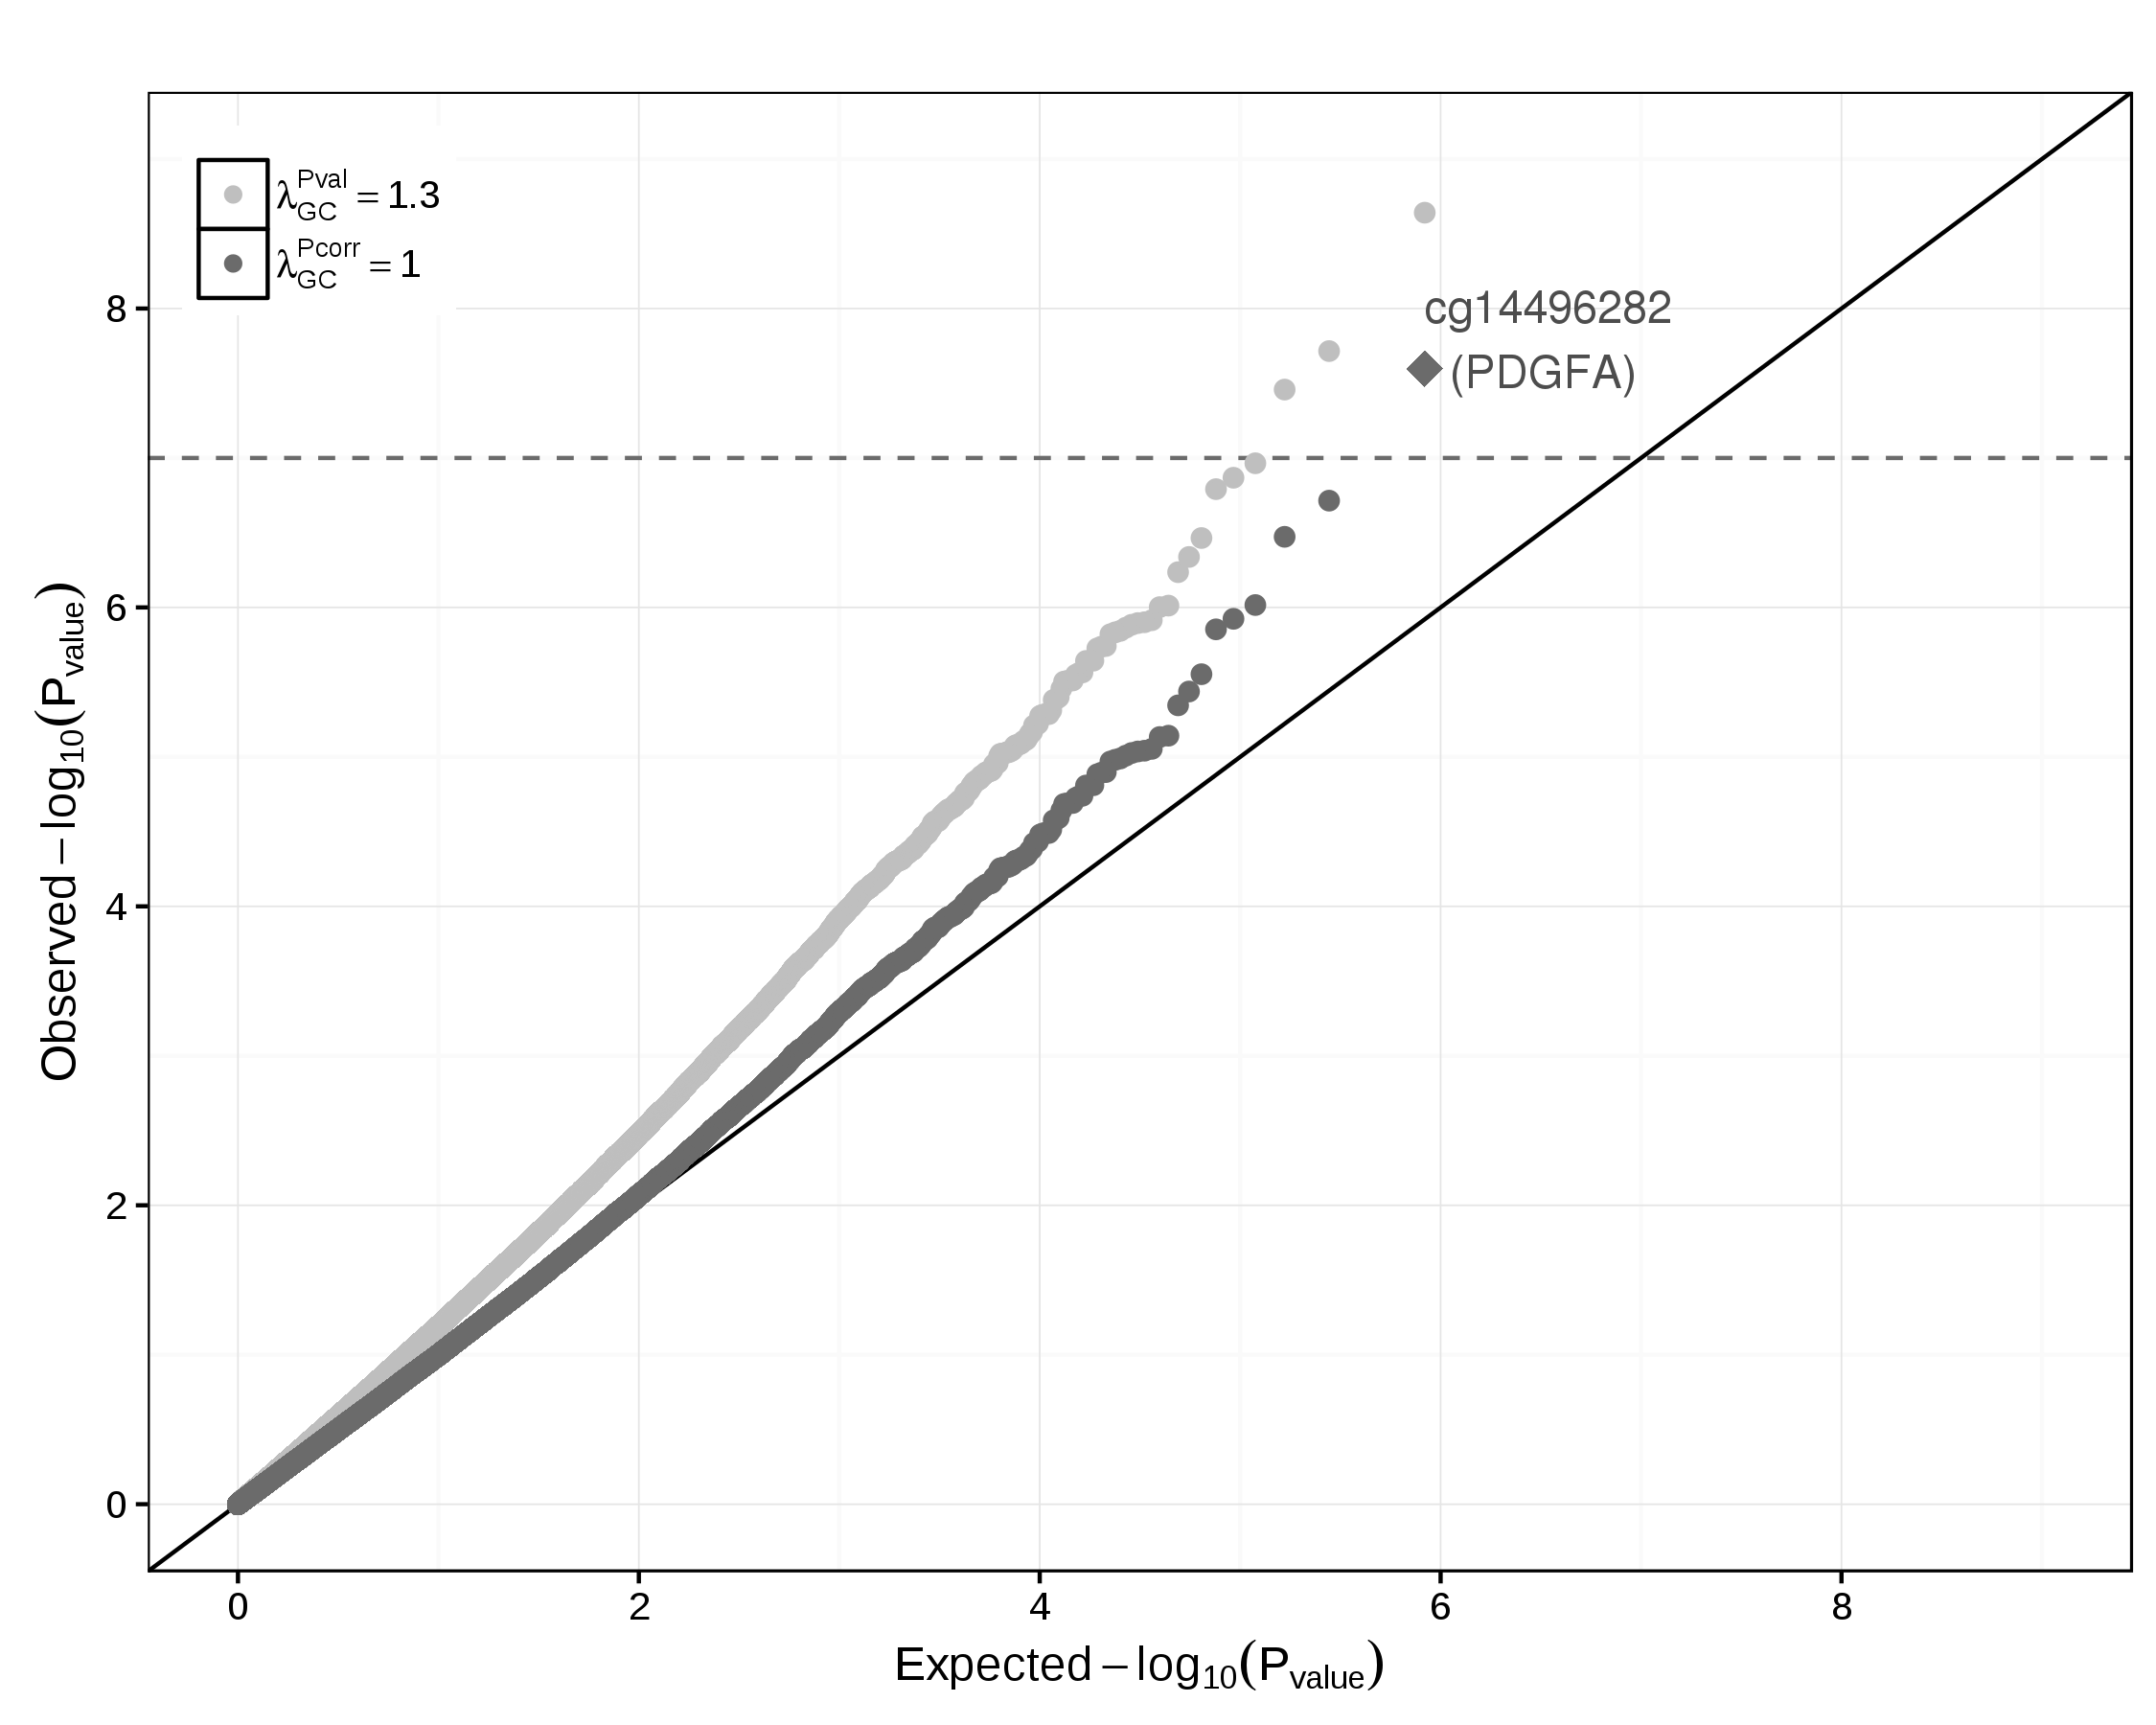
\includegraphics[width=3in,height=2.4in]{FiguresTables/Figure1_A} 

}

\caption{Graphique quantile-quantile des valeurs-p de l'étude
d'association épigénétique en cas/contrôle sur le diabète de type 2
(Chapitre \ref{Article3}), avant et après normalisation sur le facteur
d'inflation \(\lambda\). La ligne horizontale en pointillé représente le
seuil de significativité corrigé selon la méthode de Bonferroni.}\label{fig:lambda}
\end{figure}

Une fois l'analyse réalisée au moyen de logiciels tels que PLINK
\citep{chang_second-generation_2015, purcell_plink_2015}, SNPTEST
\citep{burton_genome-wide_2007, clark_conjuring_2007} ou d'extensions du
logiciel R \citep{huber_orchestrating_2015}, une correction appelée
contrôle génomique (``Genomic control'') peut être appliquée, avec comme
principale motivation la correction d'une éventuelle stratification ou
mélange au sein de la population d'étude. Cette inflation est mesurée
par le paramètre de sur-dispersion \(\lambda\) sur l'ensemble des
statistiques de test observées \citep{devlin_genomic_1999}. Il est
estimé à partir de la distribution observée des m statistiques de test
de chi-deux comparée à celle attendue sous l'hypothèse nulle. Pour se
prémunir des valeurs extrêmes, la valeur médiane (et non la moyenne) est
utilisée \(\lambda=\frac{median(\chi^2_1, \cdots, \chi^2_m)}{0,4549}\).
La distribution de la statistique de test observée dans l'étude est
ensuite corrigée par ce facteur \(\lambda\) (Figure \ref{fig:lambda}).
Il est à noter que même si le paramètre \(\lambda\) n'est pas
directement relié à la fréquence allélique, cette correction peut
toutefois engendrer une perte de puissance
\citep{georgiopoulos_power_2016}

Les études GWA consistant en la réalisation d'un grand nombre de
répétitions d'un même test statistique, il convient d'appliquer une
correction pour test multiples afin de diminuer le taux de faux-positifs
global de l'étude \citep{pearson_how_2008}. Un test statistique est dit
significatif, et son hypothèse nulle rejetée, si la valeur-p est
inférieure à un seuil \(\alpha\) déterminé en amont de l'analyse
(communément fixé à 0,05). En d'autres mots, on admettra que l'hypothèse
nulle est rejetée à tort dans 5~\% des répétitions (taux de
faux-positifs). Ce seuil de 5~\% est applicable sur un seul test
statistique~; pour un grand nombre de tests, la probabilité cumulée
d'observer un ou plusieurs faux-positifs augmente avec le nombre de
tests. Depuis la première étude GWA, la méthode de correction du seuil
\(\alpha\), choisie préférentiellement en raison de sa simplicité, est
la méthode de Bonferroni \citep{dunn_multiple_2012}. Cette méthode
suppose que les tests effectués sont indépendants entre eux, et consiste
à diviser le seuil \(\alpha\) par le nombre de tests. Par exemple, pour
500~000 tests à un seuil de 5~\%, on obtient
\(\alpha_{cor}=0,05/(500\,000)=1\times 10^{-7}\). Cependant, l'hypothèse
d'indépendance n'est pas vérifiée en raison de la présence connue de
déséquilibre de liaison entre les SNPs étudiés. D'autres méthodes de
correction existent et ont été utilisées, tels le FDR (``False Discovery
Rate'') qui consiste à estimer le taux de faux-positifs parmi tous les
résultats significatifs à un seuil pré-défini \(\alpha\)
\citep{hochberg_more_1990, van_den_oord_controlling_2008}, ou encore les
méthodes de permutation comme celles développées au sein du logiciel
PLINK \citep{chang_second-generation_2015, purcell_plink_2015}. À
l'heure actuelle, le seuil nominal communément admis de significativité
est \(\alpha_{cor}=5\times 10^{-8}\). Ce seuil de significativité
pangénomique (``genome-wide significance''), a été établi en considérant
une étude avec individus d'origine caucasienne
\citep{dudbridge_estimation_2008} et réalisée à une échelle pangénomique
d'environ 1 million de SNPs indépendants.

Enfin, les résultats d'une étude GWA, après la découverte de nouveaux
loci, peuvent faire l'objet d'une validation ou d'une réplication,
c'est-à-dire que le même modèle (ou suffisamment proche) est appliqué
dans une population indépendante à celle de l'étude initiale, mais dont
les caractéristiques populationnelles sont similaires. Pour qu'un
résultat soit validé, certaines caractéristiques doivent être obtenues
dans l'étude de réplication, telles~:

\begin{itemize}
\item
  une taille d'échantillon suffisamment grande avec puissance
  statistique estimée à au moins 80~\%, permettant ainsi de limiter le
  taux de faux-négatifs et d'augmenter la réplication des
  ``vrais-positifs'' de l'étude initiale~;
\item
  un effet dans la même direction (p.~ex. effet positif), présentant une
  valeur-p inférieure au seuil nominal \(\alpha\) de 5~\%.
\end{itemize}

Ces études de réplication, même si elles ne sont pas obligatoires,
permettent tout de même de réduire le nombre de faux-positifs rapportés
dans les résultats. Une autre approche de validation concerne les
méta-analyses
\citep{zeggini_meta-analysis_2009, evangelou_meta-analysis_2013}. Ces
méthodes permettent, soit en agrégeant les valeurs-p (méthode de Fisher)
de plusieurs études (l'étude initiale n'étant pas incluse pour éviter
d'orienter les résultats), soit en utilisant les effets estimés et leur
erreurs-types (permettant de pondérer les effets selon la taille de
l'échantillon de l'étude), de proposer une valeur-p globale et
transversale à plusieurs études, indiquant par le fait même si le
résultat de l'étude initiale est validé ou non. L'hétérogénéité des
études incluses dans la méta-analyse doit être prise en compte afin
d'éviter de tirer des conclusions erronées créées principalement par les
différences entre celles-ci.

\subsubsection{Transcriptomique}\label{transcriptomique}

Une fois complété le pré-traitement et le contrôle-qualité des mesures
de fluorescence adaptés à la plateforme utilisée (p.~ex. Affymetrix,
Illumina ou Agilent), l'approche classique consiste à identifier des
gènes différentiellement exprimés selon une ou plusieurs conditions
expérimentales. En effet, l'objectif premier des puces d'expression est
d'identifier des processus biologiques ou voies biologiques permettant
de discriminer deux ou plusieurs groupes. Les différentes puces
permettent de quantifier l'expression (quantité de mRNA) pour l'ensemble
des gènes sur le génome et les différents transcrits de ces gènes.
Cependant, d'une plateforme à une autre, les informations sur les
transcrits diffèrent aussi bien en termes de quantification que
d'annotation des sondes, c.-à-d. la localisation des sondes par rapport
aux transcrits. Il est donc difficile de comparer les mesures
d'expression entre des plateformes différentes.

La détection de gènes différentiellement exprimés s'effectue
généralement au moyen d'un modèle de régression linéaire généralisé
appliqué à chaque gène individuellement. En plus de proposer un cadre
commun d'analyse des données issues des différentes plateformes
\citep{R-limma}, l'extension R \emph{limma} propose une amélioration du
modèle en incluant, d'une part, une composante hiérarchique permettant
de prendre en compte la variabilité inter-puce, et d'autre part, une
modification de la statistique de test en régulant l'erreur-type de
l'estimateur par un paramètre de variance de chaque gène sur l'ensemble
des puces et des échantillons (paramètre estimé par une approche
bayésienne empirique). Cette amélioration accroît la stabilité de
l'inférence comparée à celle de l'approche classique obtenue par
régression linéaire \citep{smyth_linear_2004, phipson_robust_2016}. Afin
d'identifier les gènes différentiellement exprimés, le seuil de
significativité \(\alpha\) doit être défini en considérant le nombre de
tests réalisées, par exemple, au moyen d'une correction sur le FDR
(option par défaut dans (option par défaut dans \emph{limma}).





\begin{figure}[!htb]

{\centering 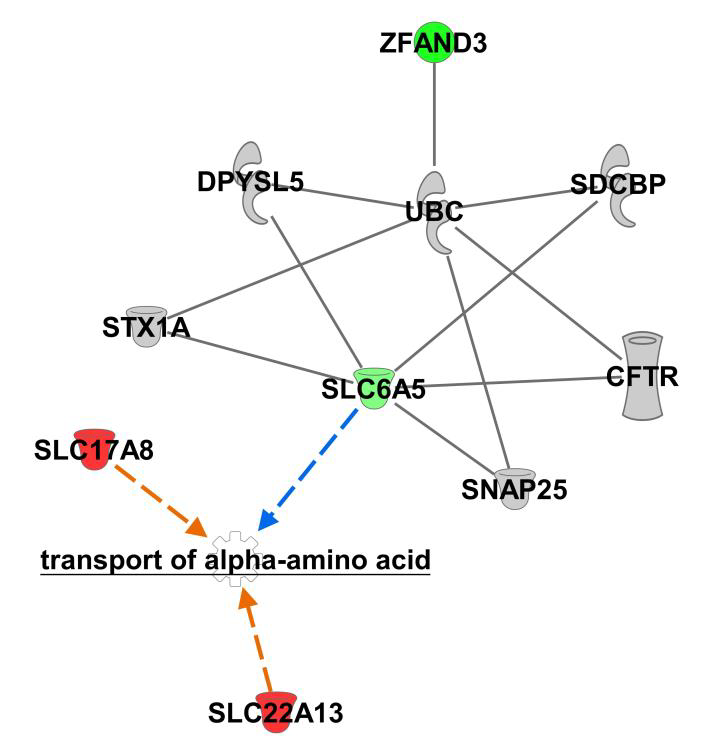
\includegraphics[width=3in,height=3.6in]{FiguresTables/networkIPA} 

}

\caption{Identification par IPA d'un réseau de gènes associé à
la diminution de l'expression de \emph{ZFAND3} (Chapitre
\ref{Article2}).}\label{fig:networkIPA}
\end{figure}

À l'issue de l'analyse, un grand nombre de gènes peut alors être
différentiellement exprimé. A priori, il est difficile d'identifier
parmi ces gènes, une fonction ou une voie métabolique commune qui
pourrait éclairer sur l'aspect biologique de ces résultats. Afin de
réduire l'information et identifier des groupes de gènes impliqués dans
une fonction particulière, une approche consiste à effectuer des tests
d'enrichissement, c'est-à-dire à évaluer si l'ensemble des gènes
présente en excès un groupe de gènes particuliers liés à une fonction ou
à une localisation dans un tissu particulier. Ces études
d'enrichissement peuvent se faire à partir de différentes bases de
données telles que ``Gene Ontology'' \citep{ashburner_gene_2000}, KEGG
(``Kyoto Encyclopedia of Genes and Genomes'')
\citep{kanehisa_kegg:_2017} ou encore depuis des logiciels d'analyse
ayant accès à leurs propres bases de connaissance comme ``Ingenuity
Pathway Analysis'' (IPA) (Figure \ref{fig:networkIPA}) et ``Gene Set
Enrichment Analysis'' (GSEA) \citep{subramanian_gene_2005}.\\
Une autre approche consiste à utiliser des méthodes de classification
hiérarchique représentées sous la forme de ``heatmap'' comportant deux
dendrogrammes, l'un représentant les dissimilarités entre les
échantillons, et l'autre celles entre les gènes/transcrits (Figure
\ref{fig:heatmap}). Cette méthode permet de visualiser rapidement et
simplement les groupes de gènes différentiellement exprimés entre
plusieurs conditions expérimentales.








\begin{figure}[!htb]

{\centering 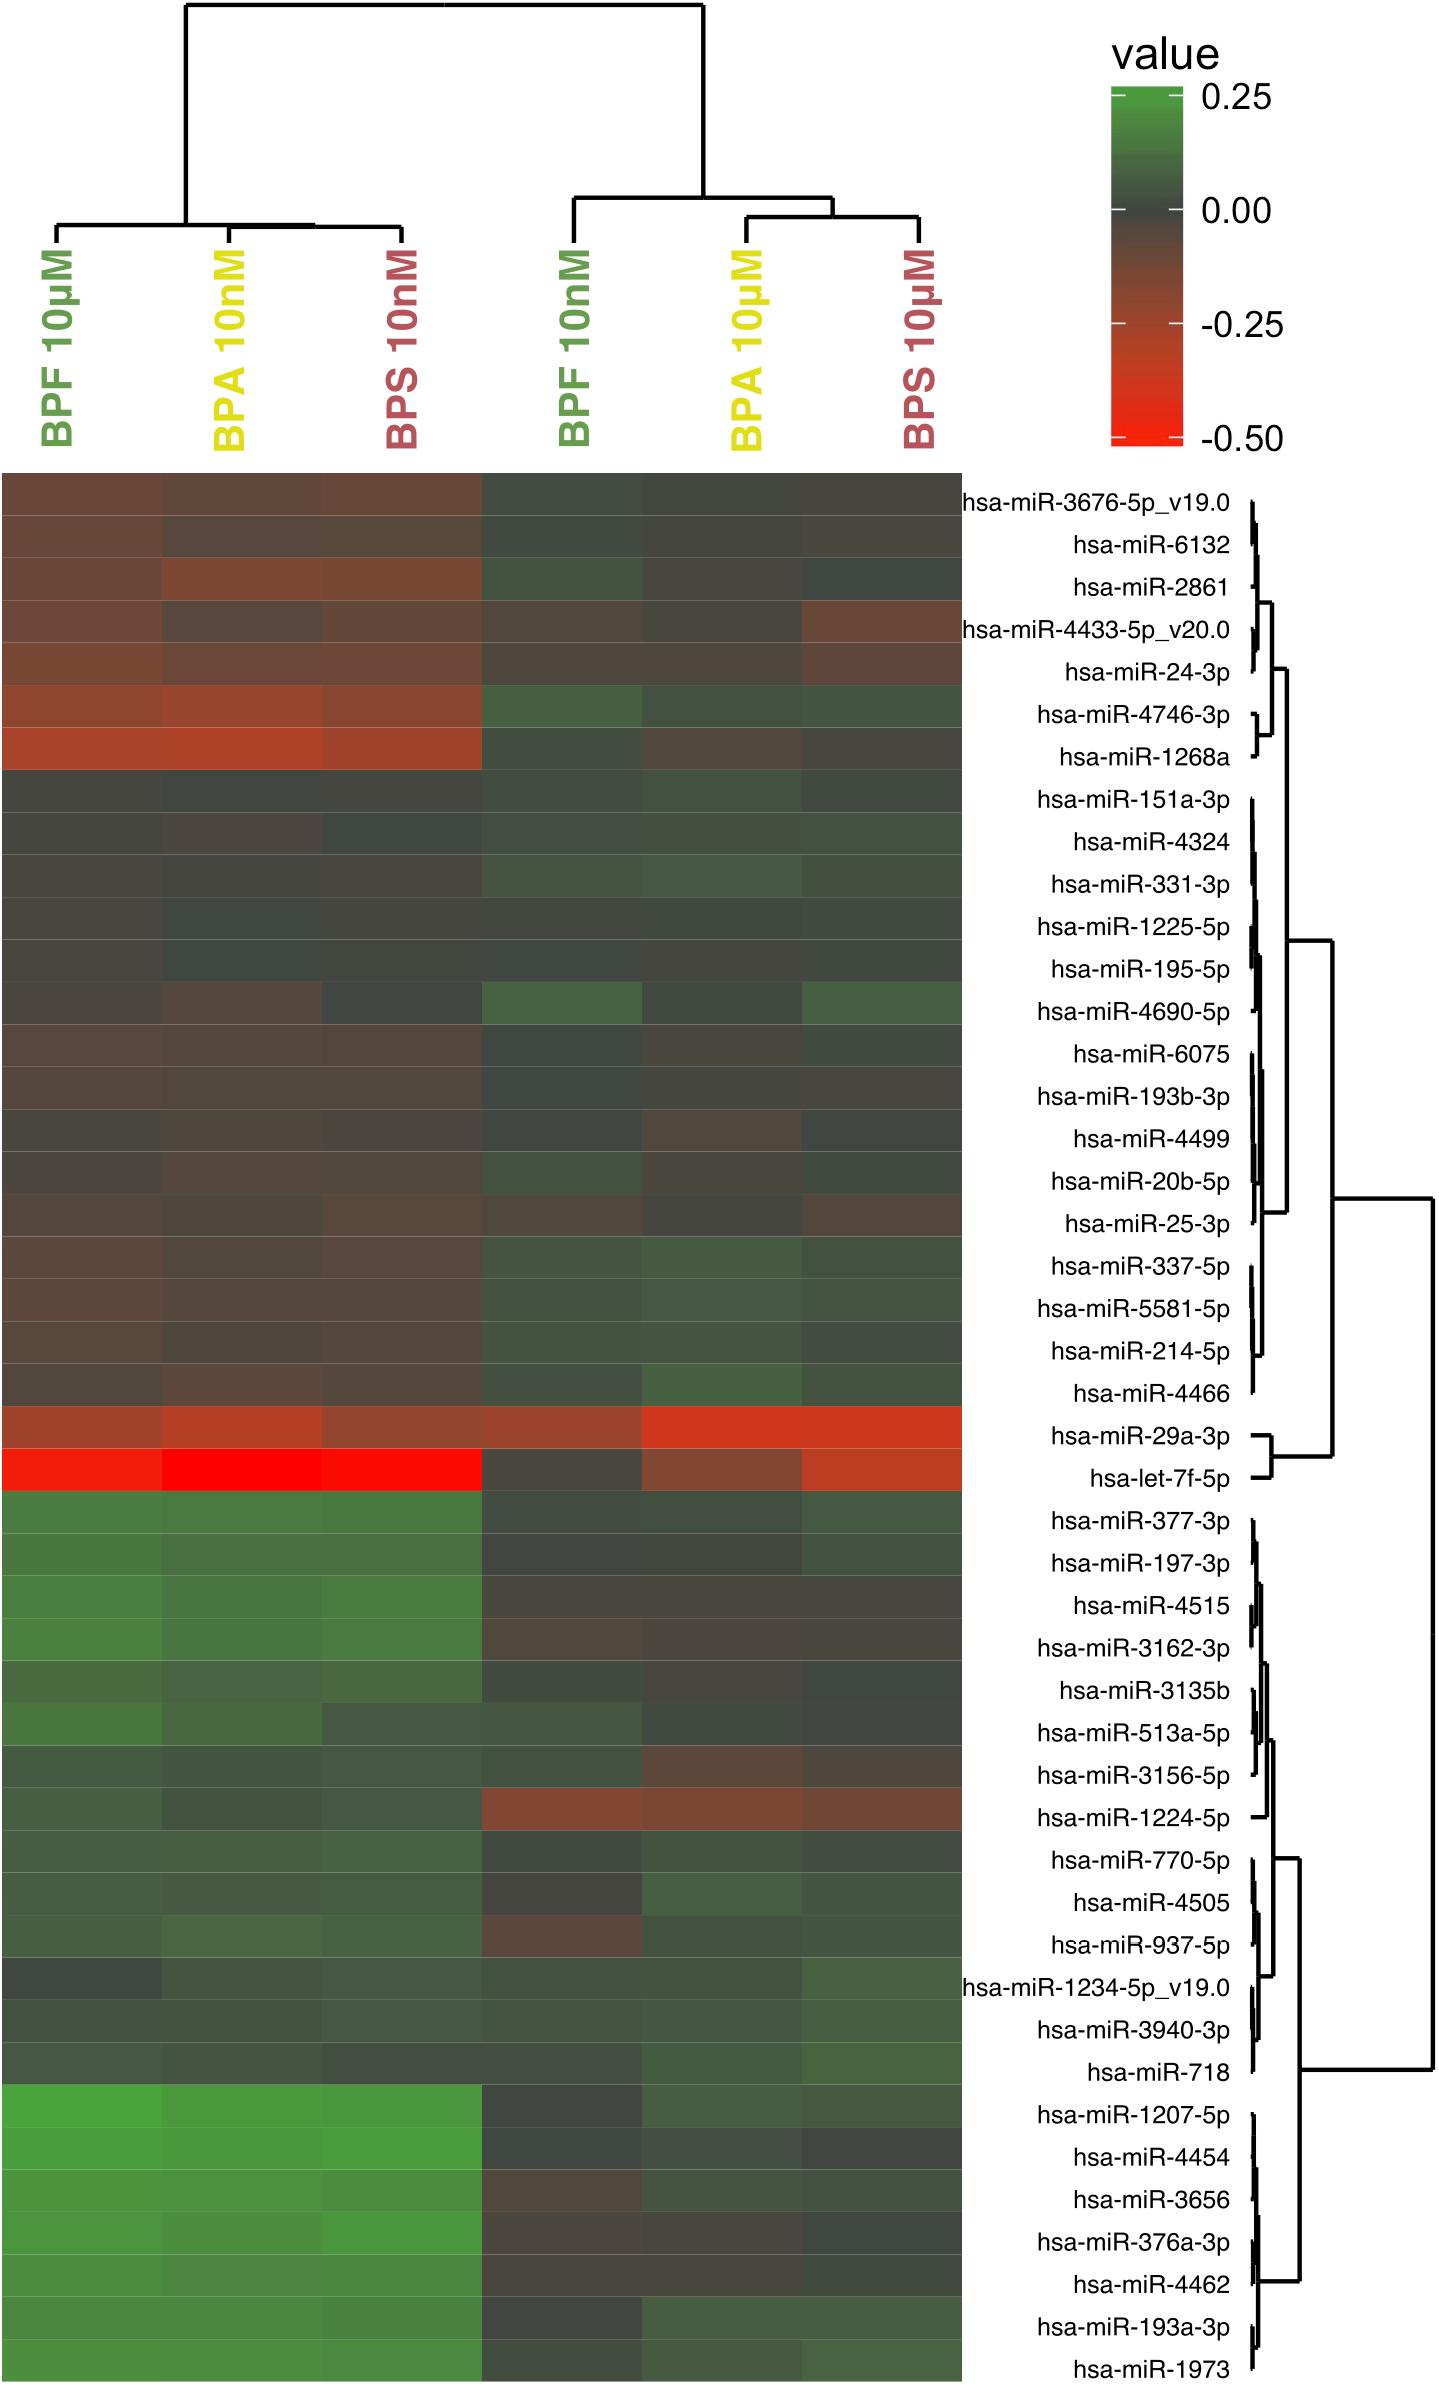
\includegraphics[width=2.5in,height=5in]{FiguresTables/heatmap} 

}

\caption{Représentation ``heatmap'' des micro ARN
différentiellement exprimés entre 10 nM et 10 \(\mu\)M, dans les 3
bisphénols (A, F et S). Les valeurs représentent les \(\log_2\) des
``Fold Change'' (c.-à-d. le ratio de l'expression d'un miRNA, pour un
bisphénol donné, sur la condition contrôle, sans exposition bisphénol)
\citep{verbanck_low-dose_2017}.}\label{fig:heatmap}
\end{figure}

\subsubsection{Méthylomique}\label{methylomique}

Après le pré-traitement des données provenant des puces de méthylation
(c.-à-d. après filtrage des sondes problématiques et normalisation des
différents biais techniques), il est possible d'analyser ces données
généralement obtenues selon un plan d'expérience de type cas/témoins.

Lorsque le plan d'expérience le permet, c'est-à-dire lorsque les
individus sont appariés entre cas et témoins, un test-t ou un test
non-paramétrique de Mann-Whitney peut être appliqué à chaque sonde. Dans
le cas contraire, les mêmes covariables d'ajustement que dans les études
GWA sont incluses dans un modèle de régression (logistique ou linéaire),
à savoir l'âge, le sexe, l'IMC, voire des composantes principales. Une
sonde est une position différentiellement méthylée (``Differentially
Methylated Position'', DMP) lorsque la valeur-p du test est inférieure
au seuil nominal de \(\alpha=0,05\) ou corrigé pour les tests multiples
(c.-à-d. Bonferroni, FDR, etc.). Les données extraites depuis le
logiciel GenomeStudio représentent les niveaux de méthylation mesurés à
chaque sonde, et rapportés en tant que valeur-\(\beta\) (suit une
distribution Bêta sous l'hypothèse que les intensités sont distribuées
selon une loi Gamma) définie comme \(\beta=\frac{M}{(M+U+\phi)}\), où
\(M\) est l'intensité de l'allèle méthylé, \(U\) est l'intensité de
l'allèle non-méthylé et \(\phi\) une constante pour compenser des
intensités sont faibles. Les valeurs-\(\beta\) varient de zéro
(complètement non-méthylé) à un (complètement méthylé). Les
caractéristiques de la distribution de ces valeurs n'en font pas une
bonne variable pour les tests statistiques (p.~ex. test-t et régression
linéaire) qui s'appuient sur l'hypothèse d'homoscédasticité de la
variable (variance constante). La transformation des valeurs-\(\beta\)
en valeurs-\(M\) (\(M=log_2\left(\frac{M+\phi}{U+\phi}\right)\)) a été
proposée et étudiée pour contourner cet écueil
\citep{du_comparison_2010}. En raison de l'interprétation biologique
simple des valeurs-\(\beta\), lesquelles sont exprimées en pourcentages,
mais de la ``qualité'' statistique des valeurs-\(M\), les analyses
statistiques sont réalisées sur les valeurs-\(M\), et ce sont les
valeurs-\(\beta\) qui sont reportées.




\begin{figure}[!htb]

{\centering 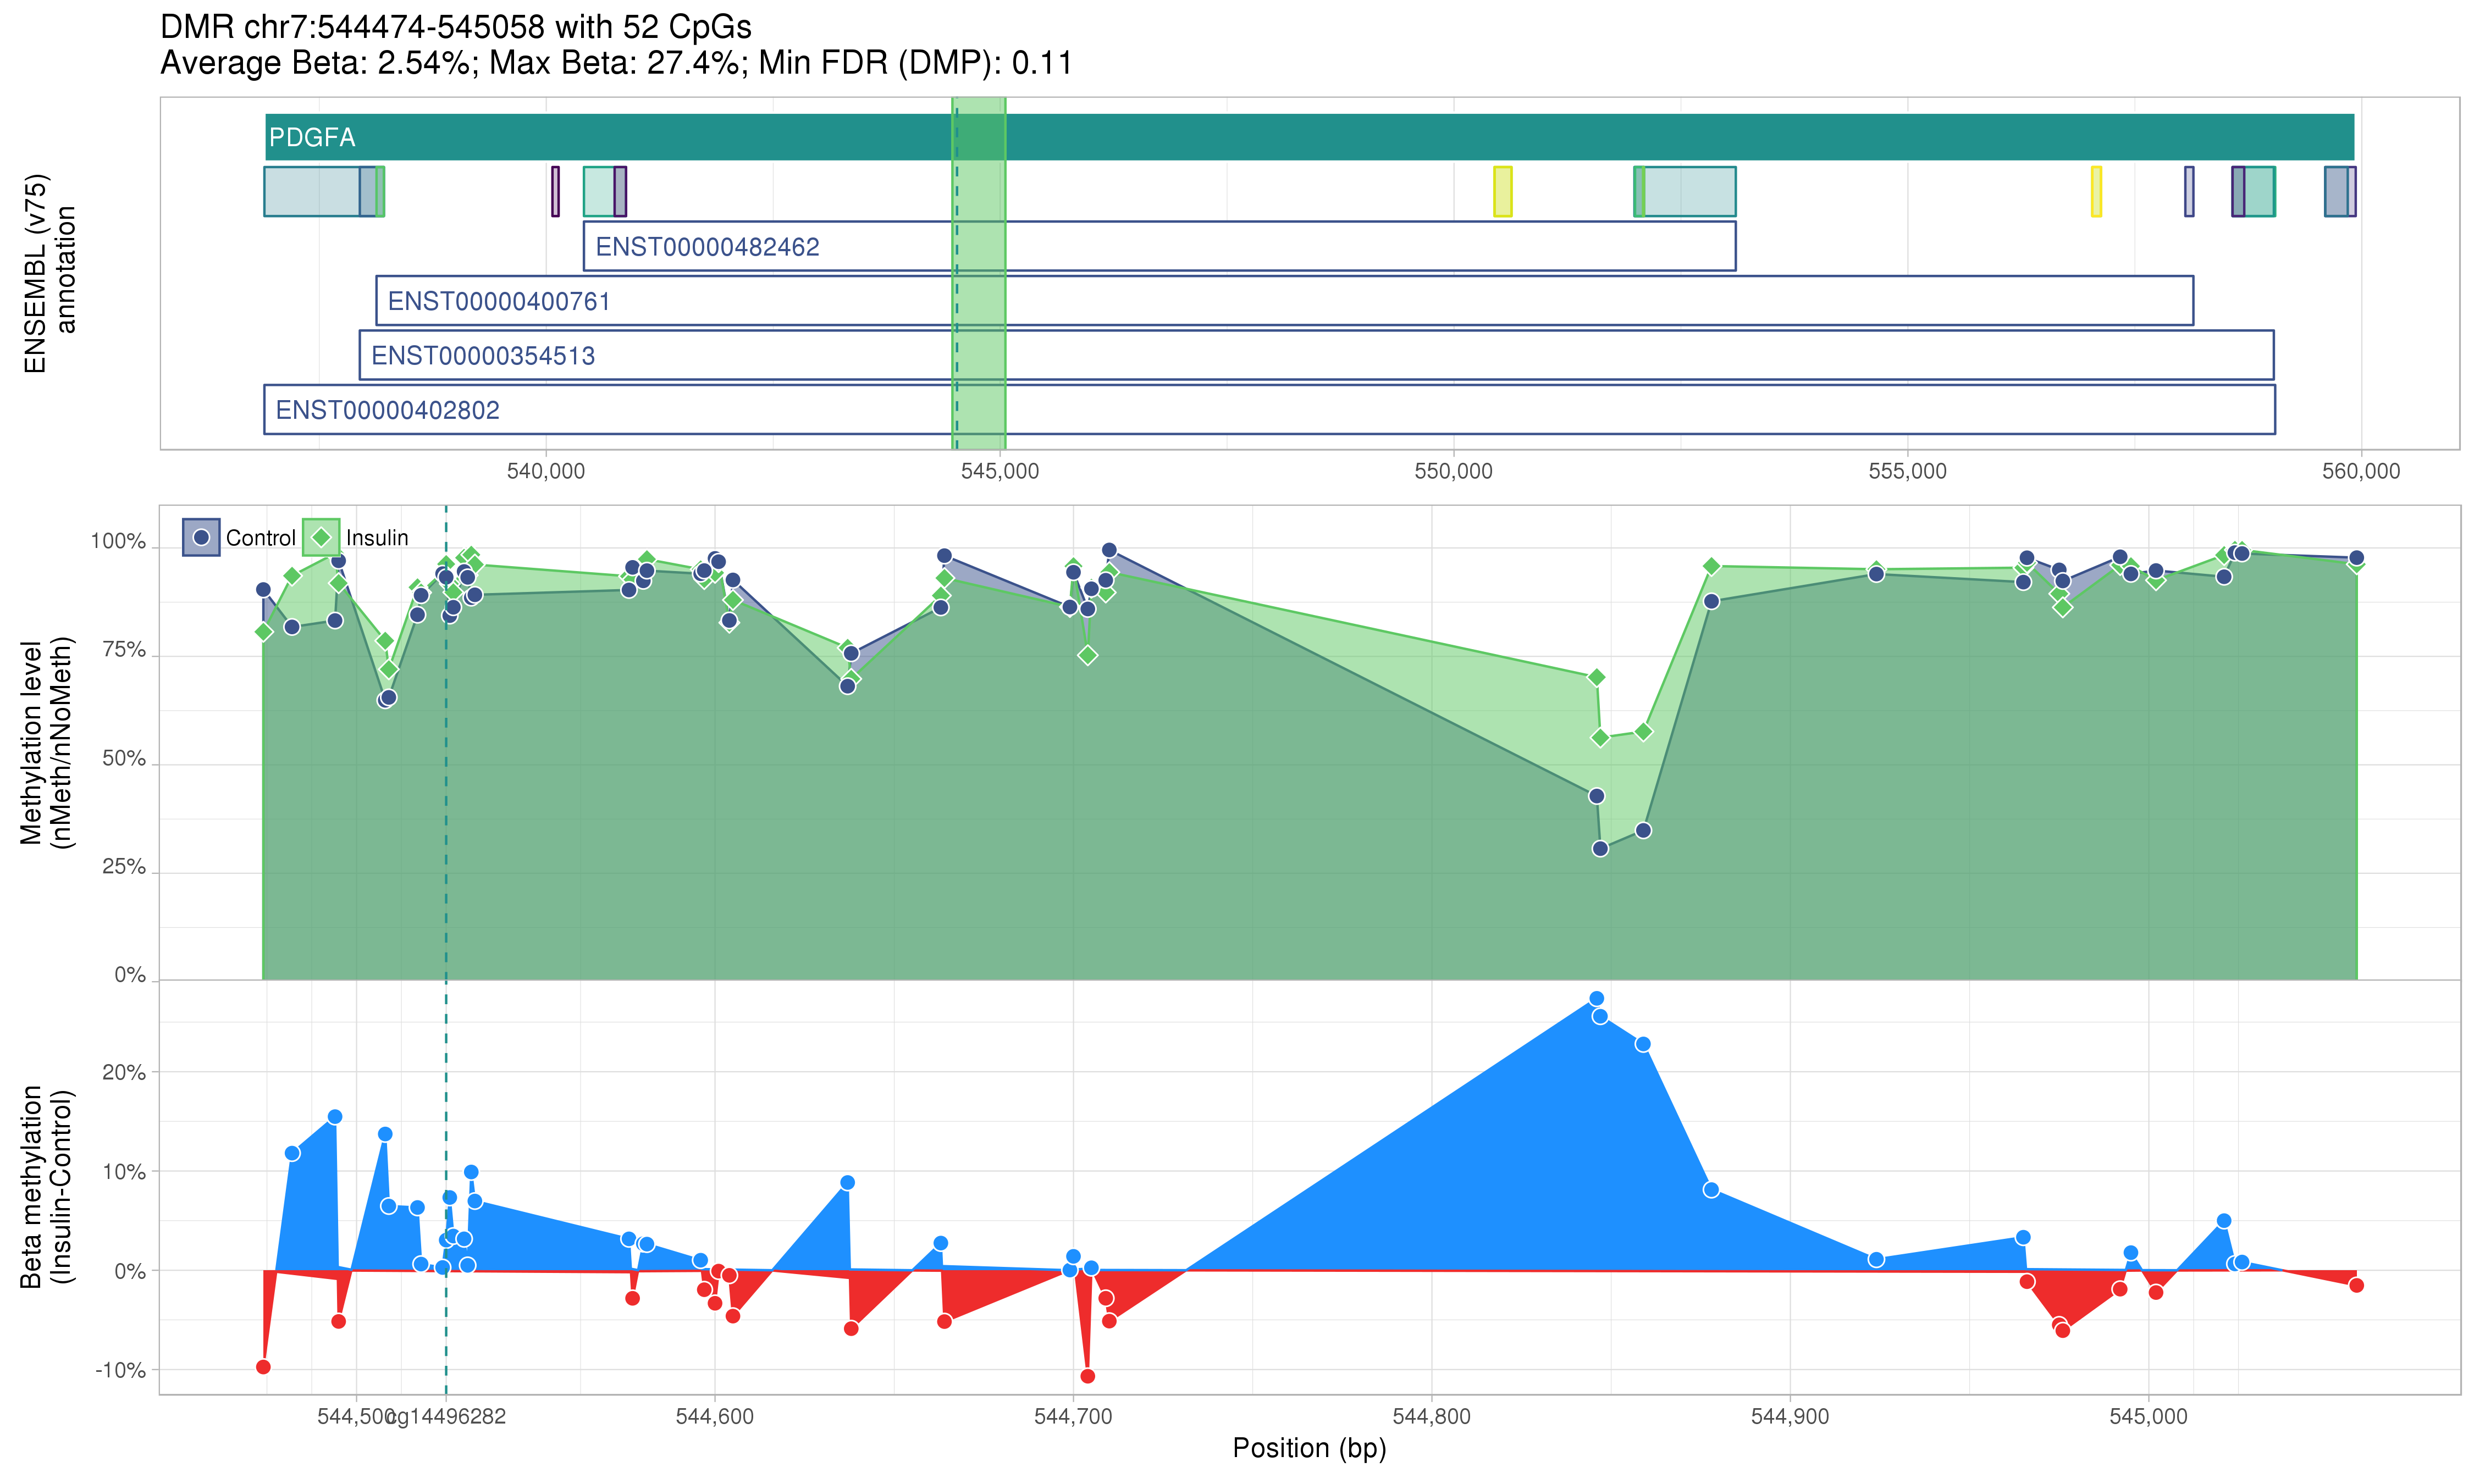
\includegraphics[width=6in,height=4.8in]{FiguresTables/DMR} 

}

\caption{Représentation de la méthylation du gène \emph{PDGFA} et du
locus CpG cg14496282 en présence d'insuline (Chapitre \ref{Article3}).}\label{fig:DMR}
\end{figure}

Une seconde approche peut être réalisée en considérant non plus chaque
sonde de façon individuelle, mais en considérant des régions ou blocs,
permettant de ce fait d'identifier des régions différentiellement
méthylées (``Differentially Methylated Region'', DMR)
\citep{peters_novo_2015, hansen_increased_2011, hansen_bsmooth:_2012}
(Figure \ref{fig:DMR}). Cette approche se base sur l'hypothèse que des
sondes dans un même voisinage auraient le même comportement en termes de
méthylation~: par exemple, une région hypométhylée ou méthylée au niveau
du promoteur de la transcription d'un gène. Cependant, en raison de la
couverture relativement faible et non-homogène du génome par la puce
Illumina HumanMethylation450 \citep{bibikova_high_2011}, cette approche
ne permet d'étudier que partiellement ces régions, et est destiné
principalement aux techniques de séquençage (p.~ex. séquençage
bisulfite) ou aux puces bénéficiant d'une plus grande couverture, comme
c'est le cas dans les dernières puces Illumina HumanMethylation850
\citep{moran_validation_2016}.

Comme dans les études GWA, une validation ou une réplication des
résultats est préconisée d'autant plus que les biais techniques (p.~ex.
types de sonde, effet plaques, etc.) représentent des facteurs majeurs
menant à une inflation du taux de faux-positifs. Une première approche
consiste à réaliser une réplication avec la même technologie sur une
cohorte indépendante présentant des caractéristiques similaires. Une
seconde approche consiste à réaliser une validation d'un DMP ou DMR à
l'aide d'une autre technologie (p.~ex. mesurer la méthylation d'un
DMP/DMR via une technique ciblée comme le pyroséquençage) sur la même
population que l'étude initiale \citep{kurdyukov_dna_2016}. Cette
dernière présente l'avantage de pouvoir valider ce qui a été observé
dans une population donnée avec une technologie donnée, et permet en
conséquence de réduire le risque de faux-positifs imputable à un facteur
technique, mais ne permet toutefois pas d'éliminer une potentielle
spécificité de la population étudiée (p.~ex. biais de sélection). En
revanche, la première approche permet de contrôler à la fois ces deux
phénomènes, lorsque la population de réplication est adaptée.





\begin{figure}[!htb]

{\centering 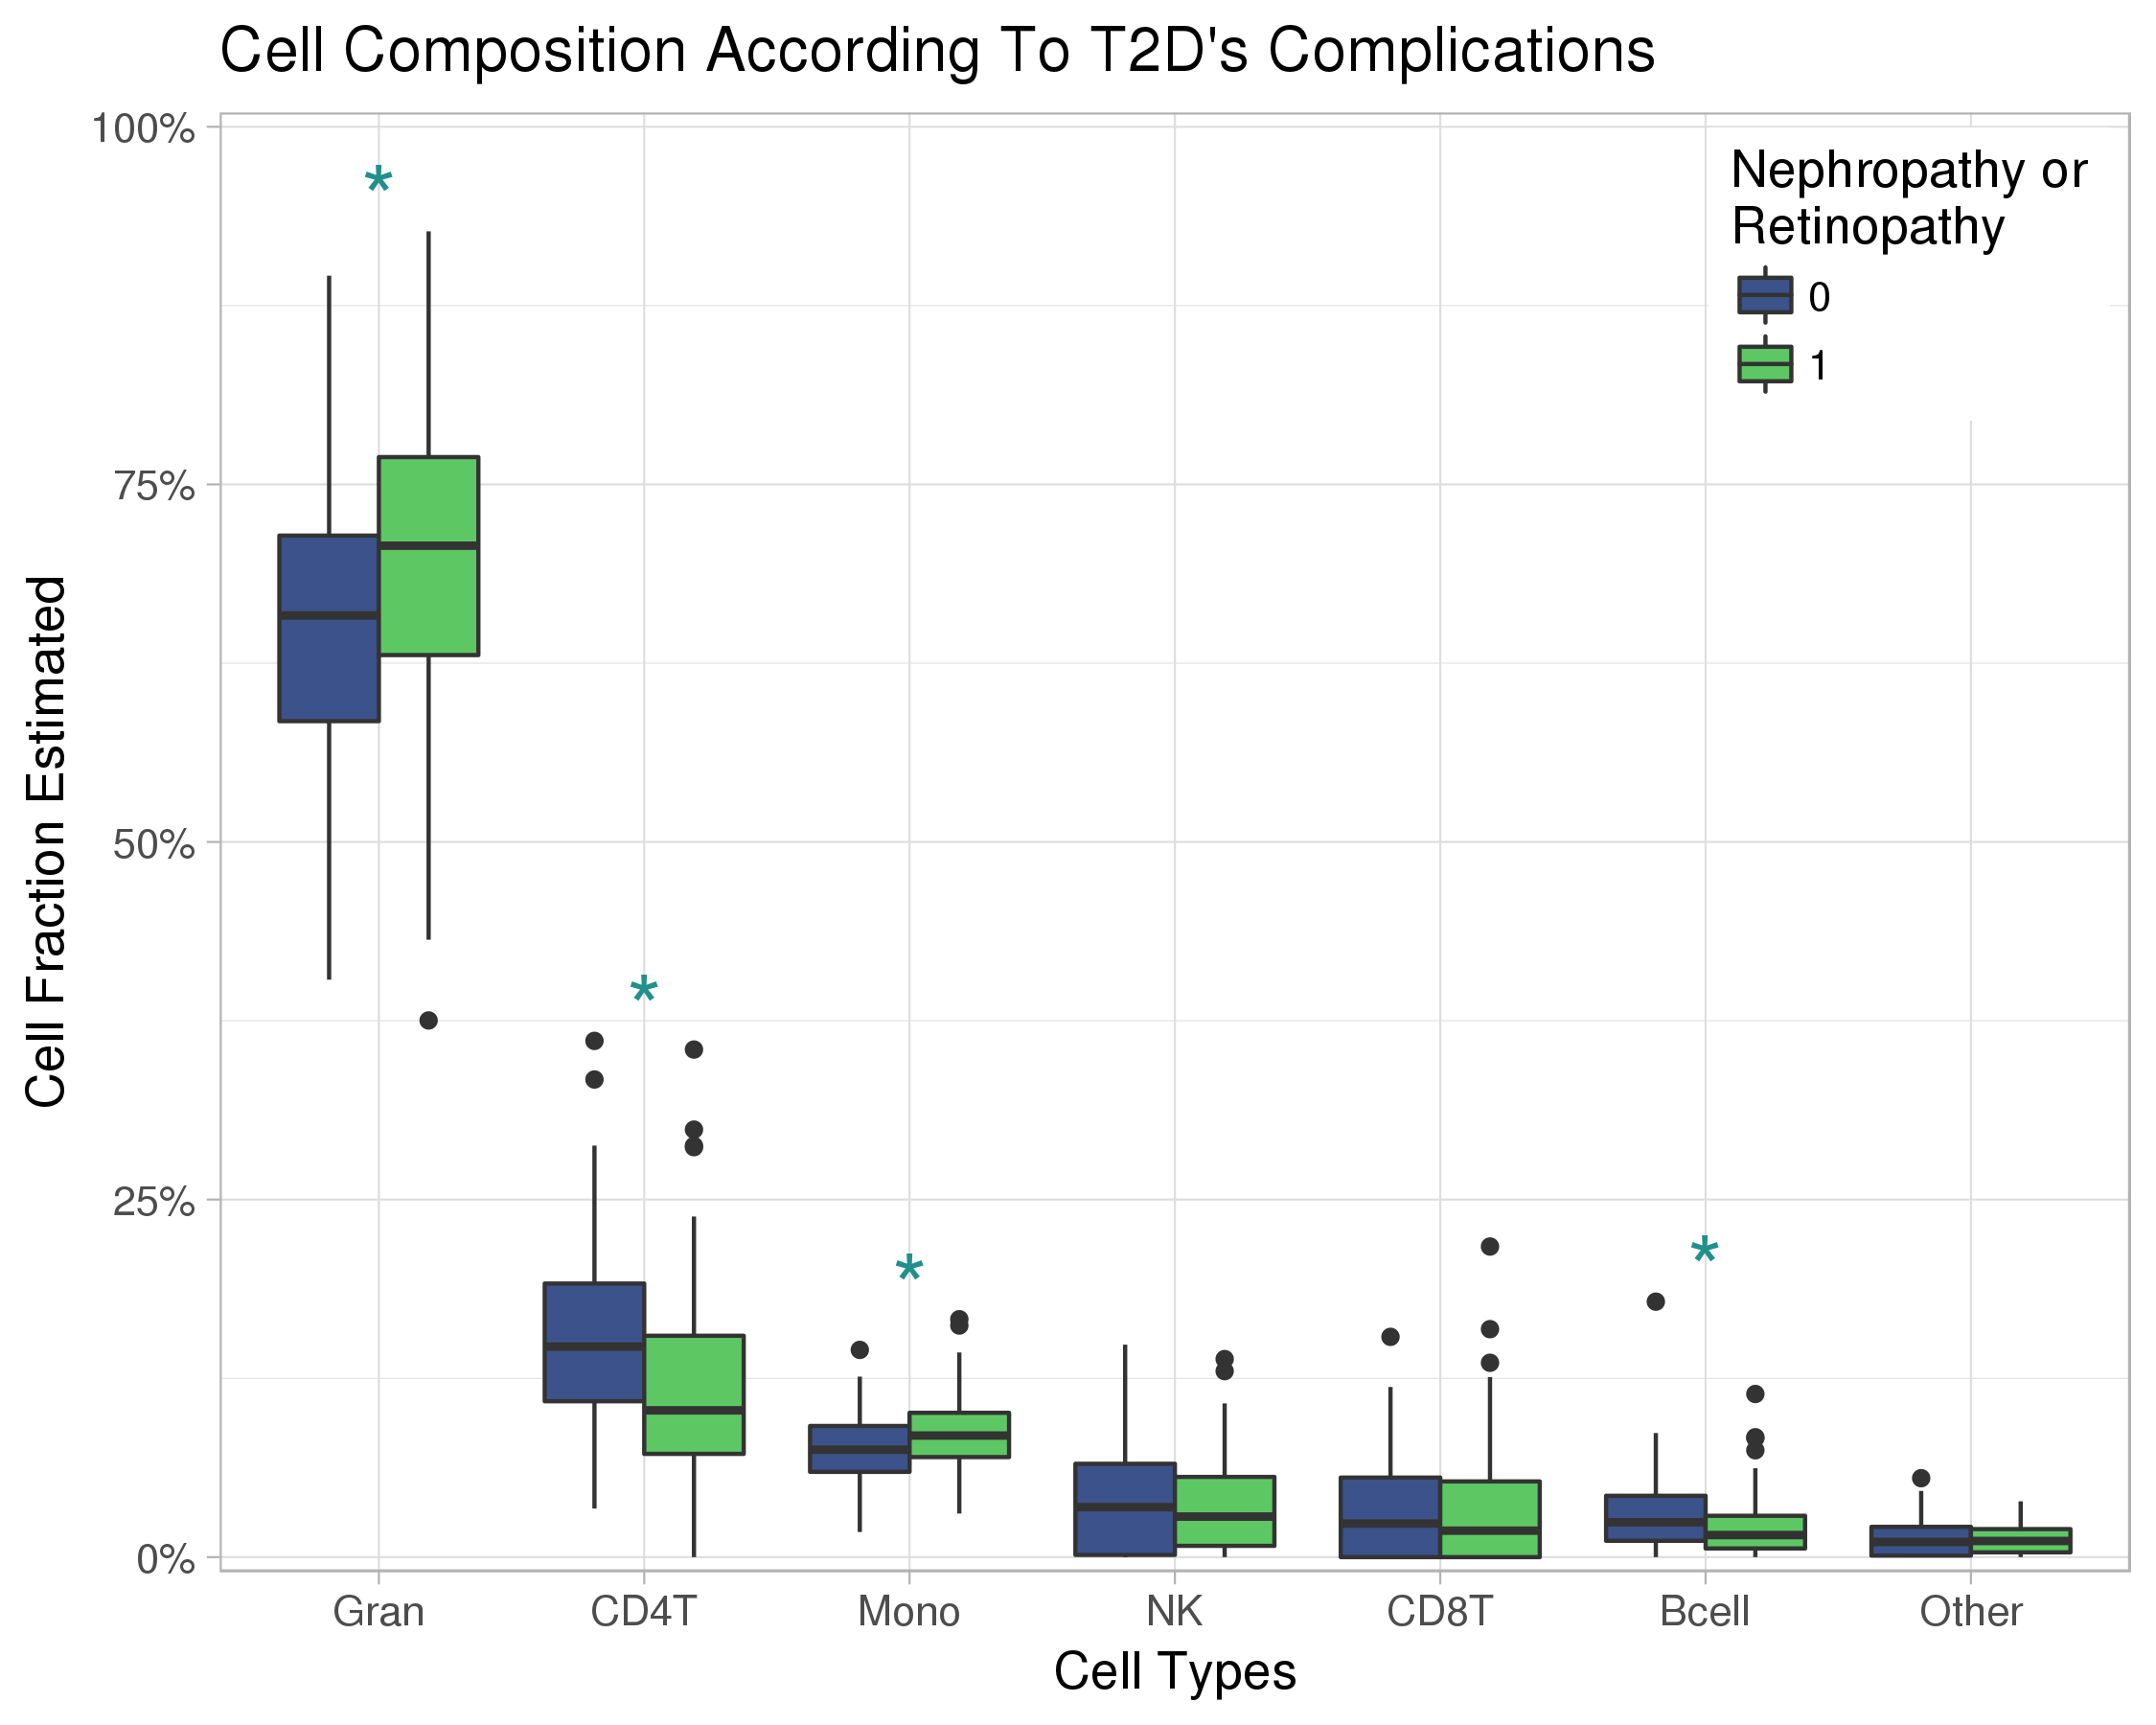
\includegraphics[width=3in,height=2.4in]{FiguresTables/Figure8} 

}

\caption{Estimation des différences de composition cellulaire
(selon une base de référence) entre le groupe diabétique et le groupe
contrôle.}\label{fig:compcell}
\end{figure}

Il est à noter que la méthylation diffère entre les tissus, et plus
précisément entre les types cellulaires. Les échantillons provenant
généralement de prélèvements sanguins, voire de biopsies, la composition
cellulaire du prélèvement, c.-à-d. le nombre et la proportion des types
cellulaires qui composent le tissu, peut ne pas être homogène d'un
individu à l'autre, et par conséquent, d'un groupe à l'autre. Ceci peut
représenter un facteur de confusion avec le statut cas/témoin d'une
étude. Il convient alors de considérer l'étude des valeurs-\(\beta\) à
l'aide d'une base de référence
\citep{houseman_dna_2012, teschendorff_comparison_2017, cardenas_validation_2016}
(Figure \ref{fig:compcell}) ou de façon algorithmique, comme s'il
s'agissait d'un mélange de distributions, par exemple, ou en effectuant
une décomposition de celles-ci sur le même principe qu'une ACP
\citep{houseman_cell-composition_2015, houseman_reference-free_2016, houseman_reference-free_2014}.
Cette différence potentielle de composition cellulaire peut également
être corrigée de la même façon que dans les études GWA, au regard de la
stratification de la population, avec notamment l'application d'une
correction post-analyse comme le contrôle génomique, simultanément ou en
plus de sa prise en compte en tant que covariable d'ajustement dans le
test d'association.

\subsubsection{Multi-omique}\label{multi-omique}

Lorsque les données de différentes omiques sont disponibles pour un
ensemble d'individus, il peut être intéressant d'intégrer ces
différentes sources d'information afin d'améliorer et de parfaire la
compréhension d'une association mise en avant lors des analyses décrites
précédemment. Lorsqu'un gène/SNP/CpG est identifié comme candidat pour
la susceptibilité au trait d'intérêt, des analyses complémentaires et
ciblées peuvent être réalisées et pourront être étudiées de façon
conjointe. La méthode employée le plus souvent consiste alors soit à
mesurer les corrélations entre les différentes données omiques, soit à
inclure cette information additionnelle en tant que covariable dans le
modèle de régression. Lorsque des puces ADN sont employées et qu'aucune
hypothèse ou sélection a priori n'est réalisée, le volume de données
devient très important et difficle à intégrer pour l'ensemble des trois
omiques discutées dans ce manuscrit (Tableau \ref{tab:omics}). Quelques
méthodes exploitant deux omiques différentes seront rapidement
détaillées dans la suite. Heureusement, des approches de type ``machine
learning'' commencent à voir le jour pour analyser tous les types de
données omiques simultanément \citep{lin_machine_2017}, données
provenant de puces ou issues de méthodes de séquençage à haut-débit dit
de nouvelle génération (\emph{Next Generation Sequencing}).




\begin{longtable}[]{@{}ccc@{}}
\caption{\label{tab:omics}Plateformes omiques (puce-à-ADN) utilisées dans les
Chapitres \ref{Article1}, \ref{Article3} et \ref{Article4}.}\tabularnewline
\toprule
Plateforme & Nombre de sondes/marqueurs & Omique\tabularnewline
\midrule
\endfirsthead
\toprule
Plateforme & Nombre de sondes/marqueurs & Omique\tabularnewline
\midrule
\endhead
Illumina HumanHT-12 & \textasciitilde{}50 000 &
Transcriptomique\tabularnewline
Agilent SurePrint G3 Human mRNA/lncRNA Microarray & \textasciitilde{}50
000 & Transcriptomique\tabularnewline
Agilent SurePrint G3 Human miRNA Microarray & \textasciitilde{}2 500 &
Transcriptomique\tabularnewline
Illumina Cardio-Metabochip & \textasciitilde{}200 000 &
Génomique\tabularnewline
Illumina HumanMethylation450 & \textasciitilde{}480 000 &
Methylomique\tabularnewline
\bottomrule
\end{longtable}

\clearpage

\paragraph{\texorpdfstring{eQTL~: ``expression Quantitative Trait
Loci''}{eQTL~: expression Quantitative Trait Loci}}\label{eqtl-expression-quantitative-trait-loci}

Quoique les études GWA aient permis d'identifier des loci de
susceptibilité, le mécanisme reliant ces SNPs à la maladie n'est pas
évident. Les analyses dites eQTL pour ``expression Quantitative Trait
Loci'' \citep{rockman_genetics_2006, gibson_quantitative_2005} proposent
d'intégrer l'information d'expression des gènes à ces loci de
susceptibilité de façon à identifier une relation de causalité entre
génomique et transcriptomique
\citep{rockman_genetics_2006, gibson_quantitative_2005}. Ces analyses
eQTL considèrent la mesure d'expression d'un gène/transcrit en tant que
trait quantitatif sur lequel le génotype d'un SNP, ainsi que des
covariables, seront régressés pour évaluer la relation entre le génotype
et l'expression. Les combinaisons de SNPs (environ 1~000~000) et de
gènes (environ 20~000), pouvant aboutir à un très grand nombre de
configurations possibles (\(\simeq10^{10}\)), ces analyses soulèvent
notamment des problèmes computationnels \citep{mackay_genetics_2009}.




\begin{figure}[!htb]

{\centering 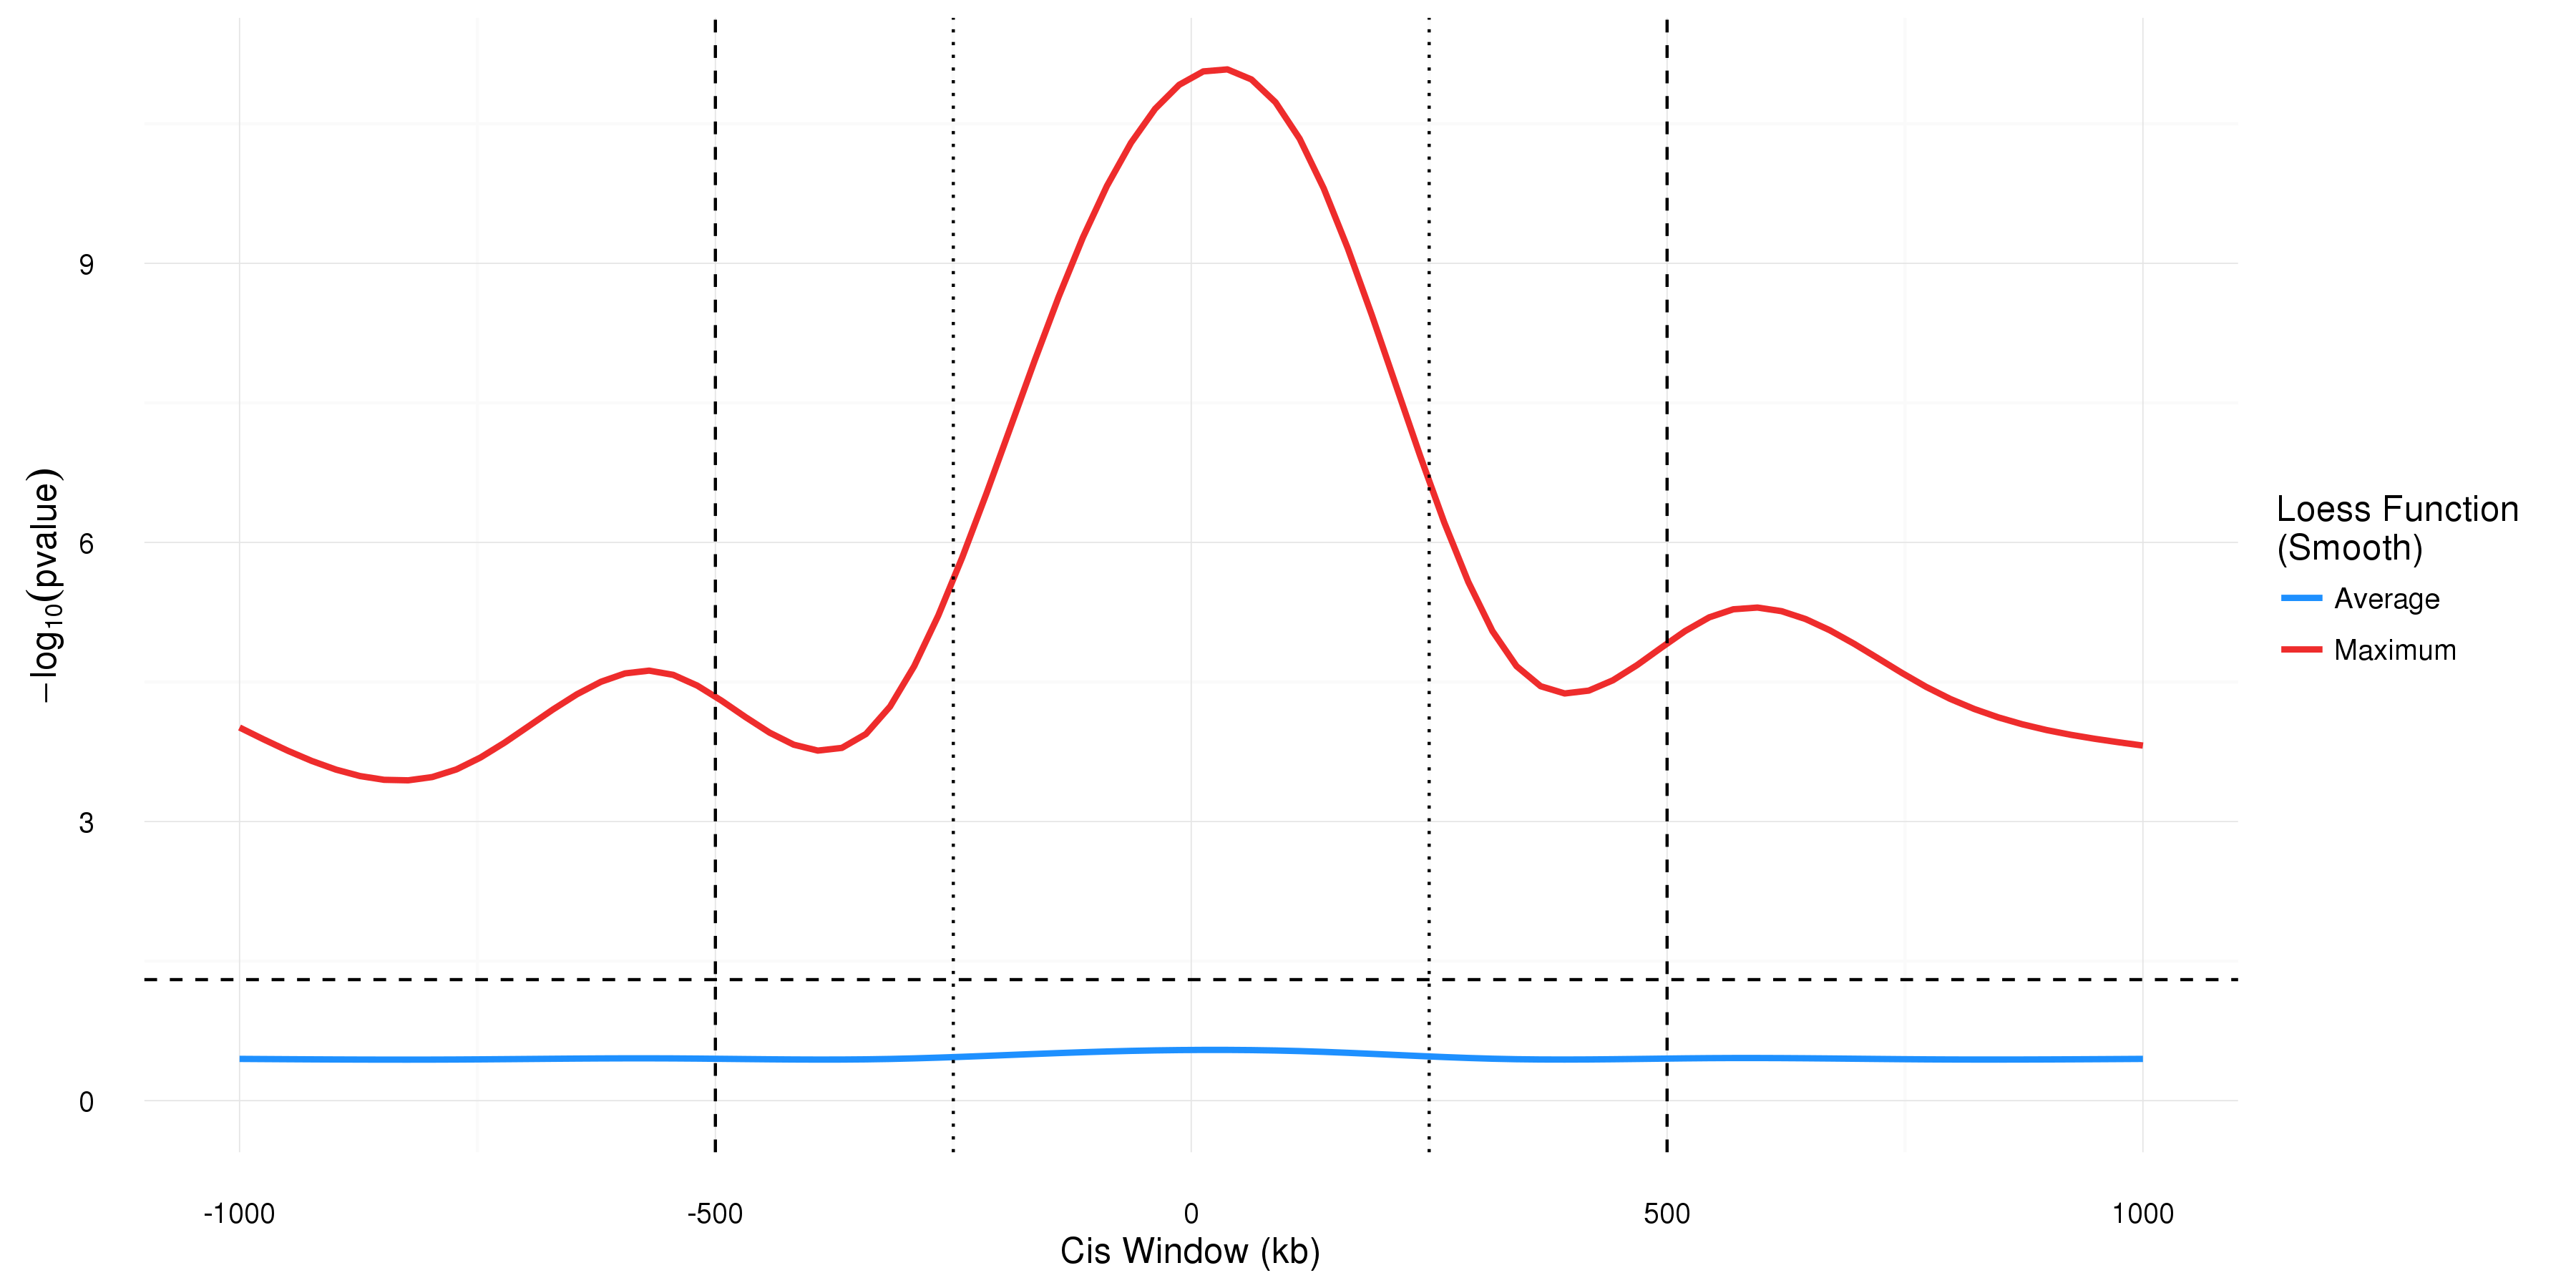
\includegraphics[width=4.8in,height=2.4in]{FiguresTables/eQTL} 

}

\caption{Distribution des valeurs-p d'association entre les SNPs et
l'expression des gènes à moins de un mégabase du promoteur du gène.}\label{fig:eQTL}
\end{figure}

Les tests peuvent être effectués en \emph{cis}, c'est-à-dire qu'un gène
est testé pour un SNP si celui-ci est localisé à moins d'une certaine
distance en paires de bases (en général, entre 100 kb et 1 Mb) du gène,
ou en \emph{trans} lorsque le SNP excède la distance définie
\citep{rockman_genetics_2006, cheung_genetics_2009}. Une façon de
définir la distance est de réaliser l'analyse sur un sous-ensemble
(aléatoire) des combinaisons à tester et d'étudier la répartition du
signal selon la distance en paire de base (Figure \ref{fig:eQTL}). Les
SNPs en \emph{trans} ne sont, en raison de contraintes computationnelles
ou d'interprétations difficiles, généralement pas analysés. En effet,
l'hypothèse courante suppose qu'un SNP a une probabilité plus élevée de
produire un effet sur l'expression d'un gène s'il se trouve dans le
corps du gène, ou en amont, c'est-à-dire proche des promoteurs de la
transcription (``Transcription Start Site'' ou TSS). Par extension,
cette approche eQTL est applicable aux données d'épigénomique et connue
sous le nom de meQTL (``methylation Quantitative Trait Loci'') ou mQTL
(utilisé parfois comme ``metabolomic Quantitative Trait Loci''), avec en
lieu et place de l'expression du gène, le niveau de méthylation d'un
site CpG.

\paragraph{Causalité~: la randomisation
mendélienne}\label{causalite-la-randomisation-mendelienne}








\begin{figure}[!htb]

{\centering 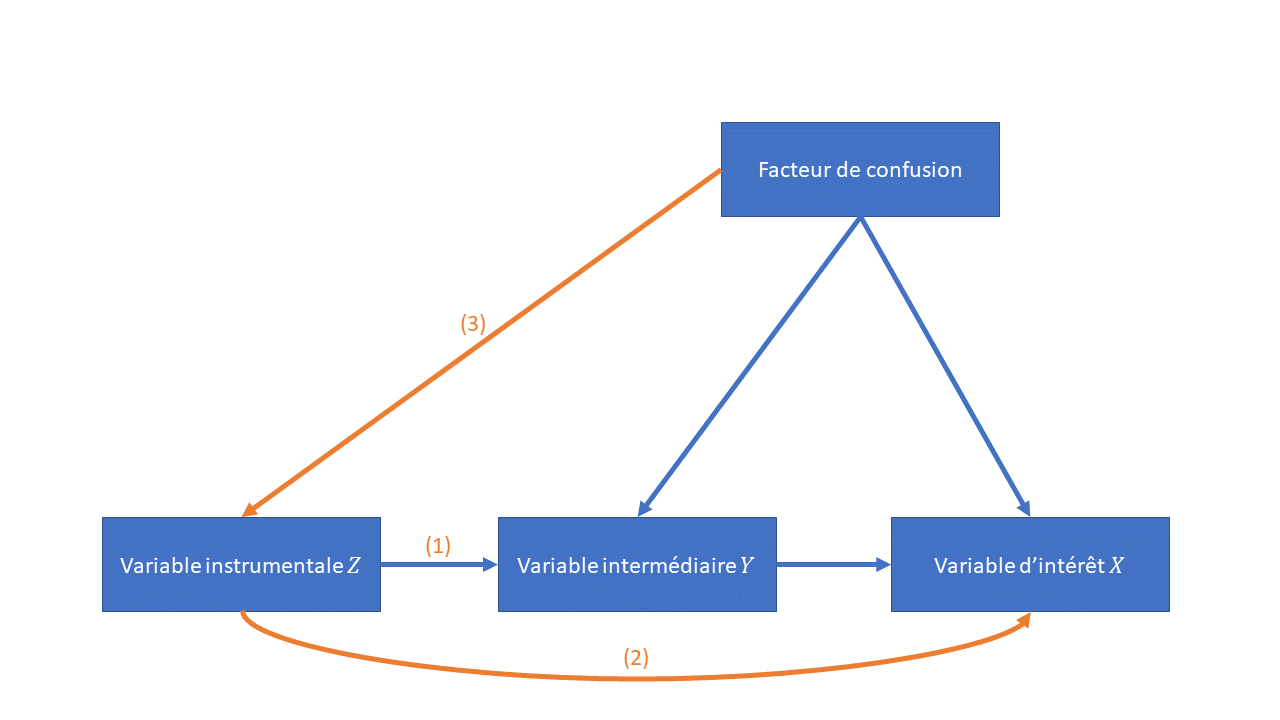
\includegraphics[width=6in]{FiguresTables/MR} 

}

\caption{Représentation schématique de la randomisation mendélienne. La
randomisation mendélienne peut être utilisée pour tester l'hypthèse
selon laquelle \(Y\) est causale de \(X\) selon que les conditions (1),
(2) et (3) soient remplies par la variable instrumentale \(Z\), où (1)
\(Z\) est associée à \(Y\), (2) \(Z\) n'est pas associée à \(X\), et (3)
\(Z\) n'est pas associé à des facteurs de confusions mesurés ou non.}\label{fig:MR}
\end{figure}

En combinant les résultats des études GWA et eQTL, il est possible
d'évaluer la causalité d'un SNP sur une pathologie en considérant que,
si un SNP est associé au risque de développement d'une pathologie et que
ce même SNP est également associé à des changements de l'expression d'un
gène (\emph{cis}), alors il est probable que le SNP soit causal de la
pathologie
\citep{nica_candidate_2010, schadt_integrative_2005, zhu_increasing_2007, chang_genome-wide_2016}.
Cette idée sous-tend la randomisation mendélienne
\citep{lawlor_mendelian_2008}, où l'expression d'un gène peut être
considérée comme un phénotype intermédiaire (\(Y\)) entre le génotype
(variable instrumentale, \(Z\)) et le phénotype d'intérêt (\(X\))
(p.~ex. statut diabétique, glycémie, insulinémie, etc.) (Figure
\ref{fig:MR}).

En général, même s'il est possible de tester l'association entre deux
variables (\(X\) et \(Y\)), il n'est pas possible de répondre quant à la
direction de cette relation~: cause ou conséquence ? En outre,
l'association entre ces deux variables peut être le résultat de facteurs
de confusion, mesurés ou non, ayant un effet sur une ou les deux
variables, causant un biais dans l'estimation de cette association. Pour
évaluer si la variable intermédiaire \(Y\) est causale de la variable
d'intérêt \(X\), la randomisation mendélienne consiste à utiliser une
variable instrumentale \(Z\), répondant aux conditions suivantes~: 1)
\(Z\) est associée à la variable intermédiaire \(Y\), 2) \(Z\) ne
présente pas d'association (directe) avec la variable d'intérêt \(X\) et
3) \(Z\) ne présente pas d'association avec des facteurs de confusion
(mesurés ou non) (Figure \ref{fig:MR}). Le génotype d'un SNP ou un score
agrégé de génotypes (p.~ex. score de risque génétique) remplit ces
conditions et permet de déduire la direction de la causalité, puisque la
génétique exerce un effet partiel ou total sur les traits biologiques,
et non l'inverse. De plus, la mesure du génotype n'est soumise qu'à peu
de variabilité et de biais. Grâce à la structure de LD entre les
variants, il n'est pas obligatoire d'utiliser le SNP causal du trait~;
un variant en fort LD avec celui-ci peut être utilisé de façon
équivalente.

\chapter*{Objectifs \& Plan}\label{objectifs-plan}


\section*{Objectifs \& Contexte}\label{objectifs-contexte}


Ce travail de thèse a été conduit au sein de l'unité de ``Génomique
Intégrative et Modélisation des Maladies Métaboliques'' UMR 8199 (CNRS /
Université de Lille 2 / Institut Pasteur de Lille) sous la direction du
Pr. Philippe Froguel et du Dr.~Ghislain Rocheleau. Le laboratoire de
``Génomique Intégrative et Modélisation des Maladies Métaboliques'',
membre de la fédération de recherche ``European Genomic Institute for
Diabetes'' (EGID), est un acteur majeur dans l'étude de la génétique du
diabète et de l'obésité, notamment par ces nombreuses publications (245
publications entre 2007 et 2017, référencées via l'outil SAMPRA de
l'Université de Lille) et la publication de la première étude
d'association pangénomique sur le diabète de type 2 en 2007
\citep{sladek_genome-wide_2007}. L'unité a développé une expertise en
génomique, transcriptomique, études fonctionnelles (modèles animaux et
cellulaires), et depuis quelques années en épigénomique, le volume et la
variété des données générées par l'unité ont donc augmenté, nécessitant
un développement méthodologique en amont (p.~ex. plan
d'étude/expérience, calcul de puissance statistique, calcul du nombre
d'échantillons nécessaire, etc.) et en aval (p.~ex. nouveau modèle
statistique, correction des biais expérimentaux et technologiques, etc.)
de la génération des données.

Ce travail de recherche s'inscrit dans un esprit pluridisciplinaire et
transversal, se situant à l'interface entre la biologie, la génétique et
la statistique, en intégrant différents types de données ``-omiques''.
Les objectifs de cette thèse consistaient à apporter un support en
statistique ainsi qu'une veille méthodologique, afin d'améliorer la
compréhension des mécanismes biologiques au moyen d'outils d'analyse
statistique adaptés et d'outils de visualisation des données
``-omiques''. Tous les résultats d'analyses de ces données, conduites en
collaboration avec des chercheurs de l'unité et des chercheurs à
l'international, ont tenté de répondre au questionnement biologique
inhérent à l'étiologie du diabète de type 2, en accord avec les besoins
identifiés par les chercheurs au sein de l'unité

\section*{Plan}\label{plan}


Différentes méthodes statistiques et types de données seront abordés au
travers de quatre chapitres, chacun correspondant à un article publié
(Chapitres \ref{Article2} et \ref{Article4}), soumis (Chapitre
\ref{Article1} et \ref{Article3}) dans des revues internationales à
comité de lecture.

Le premier chapitre porte sur le développement et l'application d'un
modèle joint permettant de modéliser conjointement deux processus
stochastiques~: d'une part, la modélisation de la trajectoire de la
glycémie à jeun chez des individus issus d'une population générale, et
d'autre part, l'évolution du risque de développement d'un diabète de
type 2, conditionnellement à la trajectoire de la glycémie à jeun. Nous
nous intéressons particulièrement à l'effet simultané des polymorphismes
(SNPs) sur ces deux processus. Le principal objectif est d'évaluer ce
modèle du point de vue de la puissance statistique, de l'erreur de type
1 et du temps de calcul, dans un contexte d'application à la génomique,
c'est-à-dire avec un volume très élevé de données. Cette évaluation est
faite, en premier lieu, sur des données simulées, puis en second lieu,
sur un jeu de données réelles générées par l'unité.

\begin{itemize}
\tightlist
\item
  ARTICLE 1~: Variants génétiques associés à la trajectoire de la
  glycémie à jeun et à l'incidence du diabète de type 2~: Une approche
  par modèle joint (Soumis à \textbf{\emph{Genetic Epidemiology}})
\end{itemize}

Le second chapitre vise à étudier l'expression des gènes de
susceptibilité au diabète de type 2, et notamment la contribution de ces
gènes dans la sécrétion d'insuline au niveau des cellules \(\beta\) du
pancréas.\\
Deux objectifs ont été remplis~: dans un premier temps, identifier les
gènes (parmi 104 candidats) étant exprimés dans l'organe clé de la
sécrétion d'insuline, soit les cellules \(\beta\) (24 tissus et types
cellulaires considérés, dont du tissu pancréatique), dans un second
temps, évaluer l'impact de ces gènes sur la sécrétion d'insuline dans un
modèle humain de cellules \(\beta\). Enfin, le séquençage de l'ARN a été
effectué pour les gènes présentant un effet sur la sécrétion d'insuline,
suivi d'une étude dans un modèle murin dont la fonction pancréatique a
été altérée.

\begin{itemize}
\tightlist
\item
  ARTICLE 2~: L'Expression et l'Évaluation Fonctionnelle des Gènes de
  Susceptibilité au Diabète de Type 2 Identifient Quatre Nouveaux Gènes
  Contribuant à la Sécrétion d'Insuline Humaine (Publié dans
  \textbf{\emph{Molecular Metabolism}})
\end{itemize}

Le troisième chapitre s'intéresse à la fois au transcriptome et au
méthylome dans une étude cas/témoins portant sur le diabète de type 2.
Dans ce chapitre, le foie est l'organe étudié, notamment pour son
implication dans la production de glucose, l'insulinorésistance
hépatique, et dans les complications souvent associées au diabète de
type 2, comme les NAFLD (``Non-Alcoholic Fatty Liver Disease''). L'étude
du méthylome a permis de mettre en évidence un site CpG (cg14496282)
localisé sur le gène \emph{PDGFA} (``Platelet-Derived Growth Factor
subunit A''), présentant une hypométhylation chez les diabétiques de
type 2. Cette hypométhylation est inversement corrélée avec l'expression
de \emph{PDGFA}, l'insulinémie et l'insulinorésistance (évalué par
l'indice HOMA-IR). Les résultats d'une étude sur un modèle d'hépatocytes
humains et de différents scores de risque génétique (\emph{Genetic Risk
Score}) suggèrent une relation causale de l'hyperinsulinémie sur le
niveau de méthylation du site CpG identifié, ouvrant ainsi la voie vers
une potentielle cible thérapeutique.

\begin{itemize}
\tightlist
\item
  ARTICLE 3~: La Surexpression Hépatique de PDGF-AA Affaiblit la
  Signalisation de l'Insuline dans le Diabète (Soumis à
  \textbf{\emph{Nature Communications}})
\end{itemize}

Le quatrième chapitre propose d'étudier les effets du bisphénol A (BPA)
et de ses substituants, soit les bisphénol F (BPF) et bisphénol S (BPS),
sur l'expression des gènes (ARN codant et non codant) dans le tissu
adipeux, et notamment les adipocytes. Le lien entre le BPA et les
désordres métaboliques comme le diabète de type 2 ayant déjà été
démontré dans des études antérieures, l'objectif consiste à mesurer au
niveau transcriptomique l'effet d'une faible concentration de bisphénol
correspondant à celle retrouvée chez l'Homme, et une concentration plus
forte qui pourrait résulter d'un relargage massif des adipocytes lors
d'une perte de poids, par exemple, ou pendant la lipolyse des adipocytes
survenant dans certaines maladies métaboliques comme le diabète de type
2.

\begin{itemize}
\tightlist
\item
  ARTICLE 4~: L'Exposition à Faible Dose aux Bisphénols A, F et S des
  Adipocytes Primaires Humains Modifie les Profils d'ARN Codant et
  Non-Codant (Publié dans \textbf{\emph{PLoS ONE}})
\end{itemize}

Enfin, une discussion générale clôt cette thèse et tente de replacer ces
travaux dans un contexte multi-omique élargi. Elle apporte des
perspectives de travail quant à l'évolution de la statistique génétique,
tributaire en partie de l'évolution des technologies permettant de
générer (encore) plus de données de différentes natures (biologique ou
informatique), en regard notamment de la diminution exponentielle des
coûts de séquençage de ces dernières années, et le développement des
études d'association portant sur les variants rares dans les populations
étudiées.

\chapter{Variants génétiques associés à la trajectoire de la glycémie à
jeun et à l'incidence du diabète de type 2 : Une approche par modèle
joint}\label{Article1}

\chaptermark{Variants génétiques associés à la trajectoire de la glycémie à jeun et à l'incidence du diabète de type 2 [...]}
Soumis à \textbf{\emph{Genetic Epidemiology}}.

\textbf{Mickaël Canouil\textsuperscript{1,2,3}}, Philippe
Froguel\textsuperscript{1,2,3,4} \& Ghislain
Rocheleau\textsuperscript{1,2,3}

\footnotesize
\textsuperscript{1}Université de Lille, UMR 8199 - EGID, F-59000 Lille,
France~; \textsuperscript{2}CNRS, UMR 8199, F-59000 Lille, France~;
\textsuperscript{3}Institut Pasteur de Lille, F-59000 Lille, France~;
\textsuperscript{4}Department of Genomics of Common Disease, Imperial
College London, London, United Kingdom. \normalsize

\section{Introduction}\label{introduction-1}

\subsection{Contexte/objectifs}\label{contexteobjectifs}

Dans le but d'optimiser l'utilisation des données phénotypiques
existantes, nous proposons une approche statistique par modèle joint
(JM) permettant l'identification de marqueurs génétiques simultanément
associés à la trajectoire temporelle d'un trait phénotypique et à la
survenue d'un événement. Nous illustrons l'application du modèle joint
dans un contexte génétique des maladies métaboliques, en exploitant la
forte association entre la trajectoire temporelle de la glycémie à jeun
et l'incidence du diabète de type 2 (DT2).

\subsection{Méthodes}\label{methodes}

Le modèle proposé dans notre étude consiste en un modèle de régression
linéaire mixte combiné à un modèle de survie dit de Cox à risque
proportionnel. À partir des données de génotypage (Illumina Metabochip
DNA arrays) obtenues pour près de 4~500 individus de la cohorte
D.E.S.I.R. (Données Épidémiologiques sur le Syndrome
d'Insulino-Résistance), nous avons analysé l'ensemble des variants
génétiques disponibles (SNPs). Sur la base de simulations faisant varier
plusieurs paramètres comme le nombre de mesures, le nombre d'individus,
la fréquence allélique et/ou le taux d'incidence, aboutissant ainsi à
240 scénarios différents (c.-à-d. 240 combinaisons des valeurs possibles
pour chaque paramètre) chacun simulés 500 fois, l'erreur de type I, la
puissance statistique et les estimations obtenues ont fait l'objet d'une
étude comparative entre l'approche par modèle joint et les approches
classiques utilisées dans les études d'association pangénomiques (GWAS).

\subsection{Résultats}\label{resultats}

Nos résultats démontrent la forte association entre la glycémie à jeun
et l'incidence du DT2 (ce qui était attendu selon la définition clinique
du DT2), et confirment également l'association entre la glycémie et
certains SNPs rapportés dans les études de type GWAS, tels que les SNPs
situés dans les gènes \emph{G6PC2} ou encore \emph{TCF7L2}. Les
associations relevées ici sont pour la plupart nominales
(\(\textrm{valeur-p} < 0,05\)), principalement en raison de la faible
taille de notre cohorte en comparaison aux tailles d'effectifs rapportée
en méta-analyse, et aussi en raison du nombre peu élevé de cas de DT2
incident (environ 5~\% sur 9 ans de suivi dans la cohorte D.E.S.I.R.).
Notre analyse par modèle joint a révélé que les SNPs se situant près ou
dans le gène \emph{MTNR1B} pourraient ne pas avoir d'effet simultané sur
l'élévation de la glycémie à jeun et le risque de survenue du DT2.

Notre étude comparative des différents modèles révèle que l'approche JM
pourrait être plus puissante, en comparaison des approches transversales
(c.-à-d. régression linéaire et logistique), pour détecter des effets de
polymorphisme, aussi bien sur le trait longitudinal (paramètre
\(\gamma\)) que sur le risque de survenue d'un événement (paramètre
\(\alpha\)), tout en maintenant l'erreur de type I près du niveau global
de 5~\%. En outre, nous avons pu observer que l'approche en deux-étapes
(``Two-Step'' ou TS) présentait une puissance et une erreur de type I
similaires à celles obtenues avec l'approche JM.

L'étude du RMSE (\emph{Root Mean Square Error}) montre que l'estimation
de \(\alpha\) est impactée par le nombre d'individus et la fréquence du
polymorphisme, mais reste similaire entre l'approche JM et l'approche
par modèle linéaire mixte. Les valeurs de RMSE divergent selon les
méthodes, notamment pour l'estimation de \(\beta\) (effet de la
trajectoire sur le risque d'événement)~: le modèle de Cox avec
covariable dépendante du temps fournit les valeurs de RMSE les plus
élevées sur l'ensemble des scénarios. Les valeurs de RMSE de l'approche
TS tendent à se rapprocher de celles de l'approche JM, particulièrement
lorsque le nombre de mesures longitudinales augmente. Dans le cas du
paramètre \(\alpha\), les valeurs de RMSE se montrent sensibles au
nombre d'individus (\(<1\,000\)), au faible nombre d'événements (taux
d'incidence \(<2,5\,\%\)), et à la fréquence du polymorphisme
(\(<5\,\%\)). Dans ces scénarios de faible fréquence allélique, faible
taux d'incidence ou petit nombre d'individus, l'approche JM présente les
valeurs de RMSE les plus faibles comparativement aux approches TS et
Cox, ces différences tendant à s'estomper lorsque le nombre d'individus
est supérieur à 2~500, ou que la fréquence allélique est supérieure à
5~\%. Enfin, la maximisation de la vraisemblance jointe de l'approche JM
se révèle être consommatrice de temps, à hauteur d'un facteur de 30 à 40
fois le temps de calculs requis par l'approche TS.

\subsection{Conclusion}\label{conclusion}

L'analyse par modèle joint a montré, d'une part, une grande cohérence
avec les résultats des études antérieures de type GWAS, et d'autre part,
semble indiquer un gain de puissance statistique pour détecter l'effet
d'un SNP sur l'évolution de la glycémie à jeun et/ou sur la survenue du
DT2. Cependant, l'approche JM présente un frein important dû au temps de
calcul énorme qui ne permet pas l'exploration systématique de tous les
SNPs à une échelle pangénomique. L'approche TS ayant montré des
caractéristiques (estimation, puissance et erreur de type I) proches de
celles de JM, et réalisable dans un temps raisonnable, pourrait être
employée comme un filtre sur les polymorphismes. Dans un second temps,
un affinage des estimations pourrait s'obtenir au moyen de l'approche
JM. Enfin, le résultat obtenu pour le gène \emph{MTNR1B} tend à montrer
qu'une modélisation statistique simultanée des deux processus pourrait
mener à une identification plus fine des variants génétiques associés à
l'homéostasie du glucose sanguin ou à la physiopathologie du diabète.

\section{Article}\label{article}

\clearpage

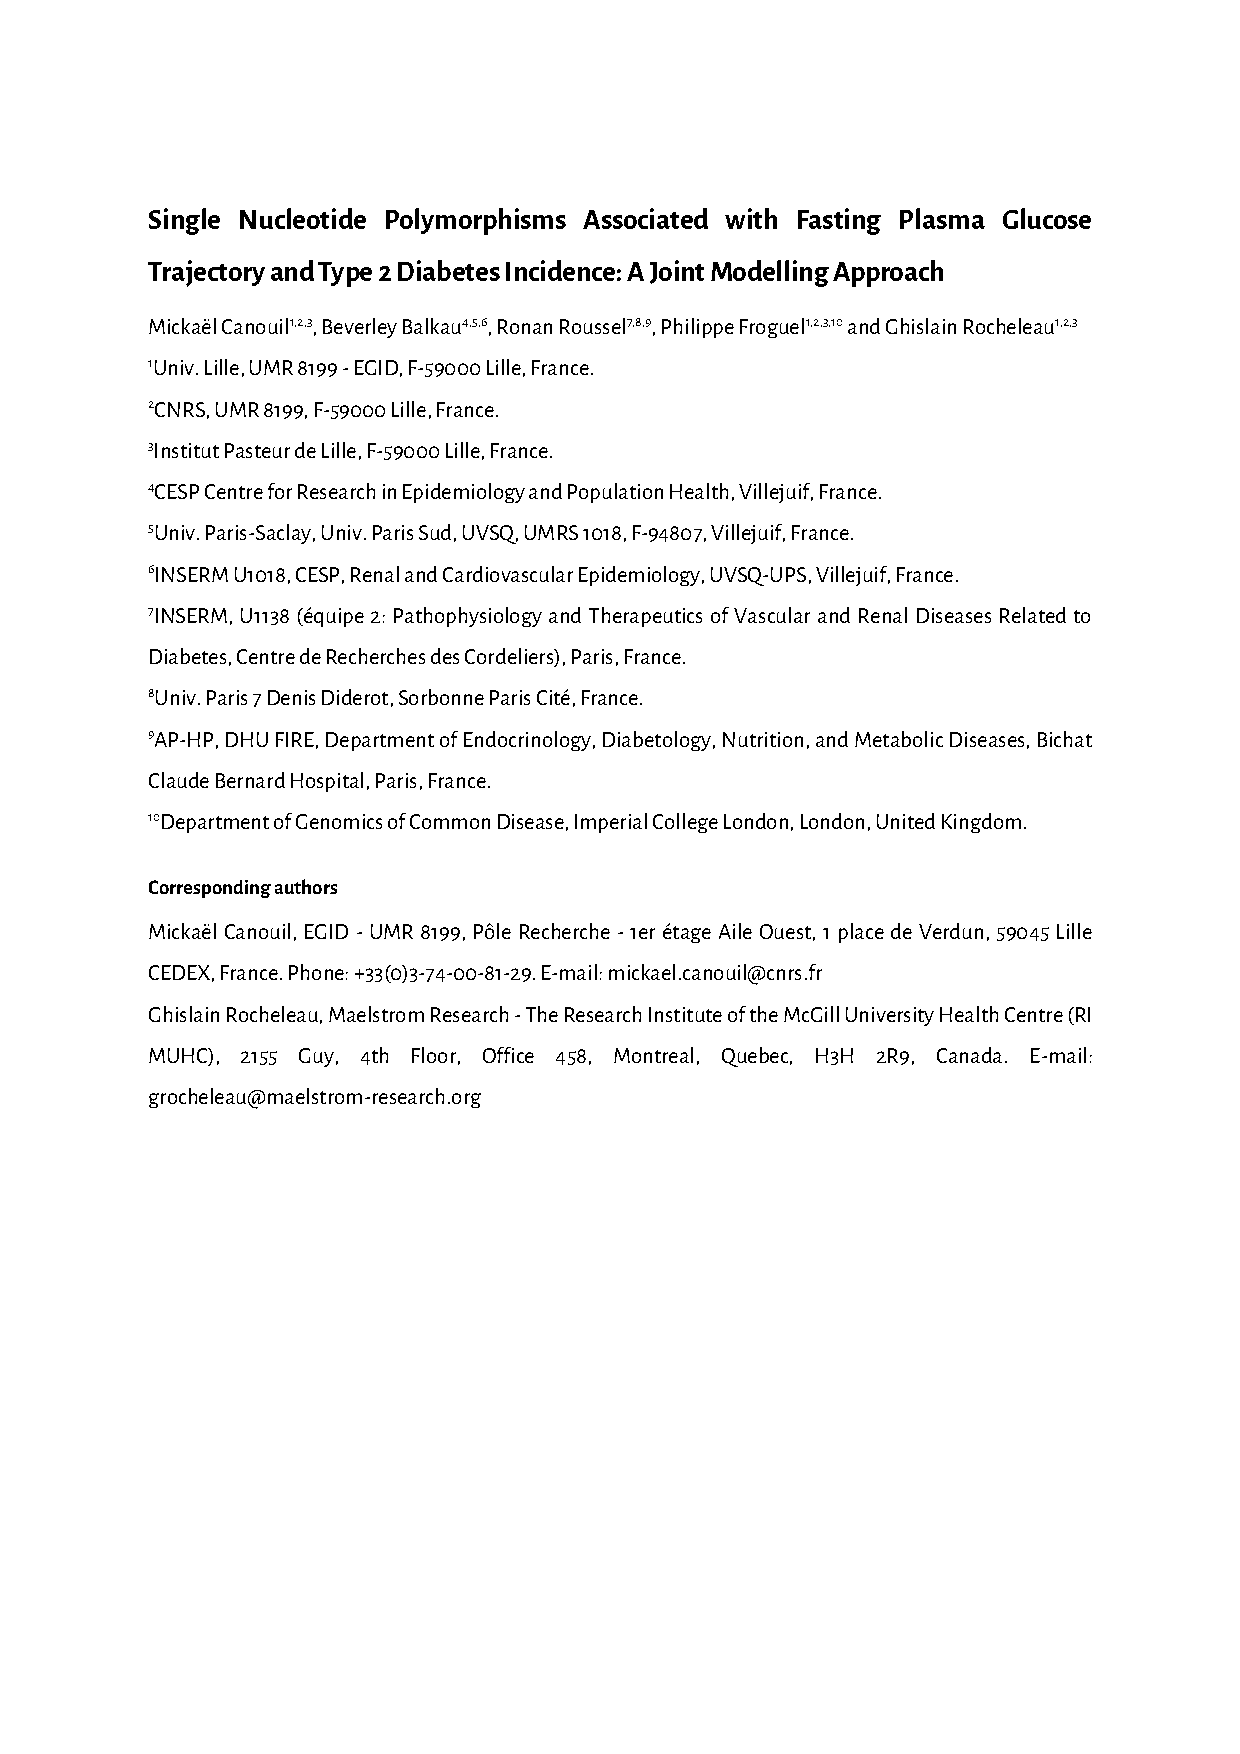
\includepdf[pages=1-12, scale=1, fitpaper=true, offset = 0cm -0.3cm, pagecommand={\thispagestyle{headings}}]{Articles/Article1.pdf}
\includepdf[pages=13, scale=1, fitpaper=true, angle=90, offset = 0cm -0.3cm, pagecommand={\thispagestyle{headings}}]{Articles/Article1.pdf}
\includepdf[pages=14-, scale=1, fitpaper=true, offset = 0cm -0.3cm, pagecommand={\thispagestyle{headings}}]{Articles/Article1.pdf}

\chapter{L'Expression et l'Évaluation Fonctionnelle des Gènes de
Susceptibilité au Diabète de Type 2 Identifient Quatre Nouveaux Gènes
Contribuant à la Sécrétion d'Insuline Humaine}\label{Article2}

\chaptermark{L'Expression et l'Évaluation Fonctionnelle des Gènes de Susceptibilité au Diabète de Type 2 [...]}
Publié dans
\textbf{\emph{\href{http://doi.org/10.1016/j.molmet.2017.03.011}{Molecular Metabolism}}}.

Fatou K Ndiaye\textsuperscript{1,\textasteriskcentered}, Ana
Ortalli\textsuperscript{1,\textasteriskcentered}, \textbf{Mickaël
Canouil\textsuperscript{1,\textasteriskcentered}}, Marlène
Huyvaert\textsuperscript{1}, Clara Salazar-Cardozo\textsuperscript{1},
Cécile Lecoeur\textsuperscript{1}, Marie Verbanck\textsuperscript{1},
Valérie Pawlowski\textsuperscript{1}, Raphaël Boutry\textsuperscript{1},
Emmanuelle Durand\textsuperscript{1}, Iandry
Rabearivelo\textsuperscript{1}, Olivier Sand\textsuperscript{1}, Lorella
Marselli\textsuperscript{2}, Julie Kerr-Conte\textsuperscript{3}, Vikash
Chandra\textsuperscript{4}, Raphaël Scharfmann\textsuperscript{4}, Odile
Poulain-Godefroy\textsuperscript{1}, Piero Marchetti\textsuperscript{2},
François Pattou\textsuperscript{3}, Amar
Abderrahmani\textsuperscript{1,5}, Philippe
Froguel\textsuperscript{1,5,\textdagger} \& Amélie
Bonnefond\textsuperscript{1,5,\textdagger}

\footnotesize
\textsuperscript{1}CNRS UMR 8199, European Genomic Institute for
Diabetes (EGID), Institut Pasteur de Lille, University of Lille, 59000
Lille, France~; \textsuperscript{2}Department of Clinical and
Experimental Medicine, Islet Cell Laboratory, University of Pisa, 56100
Pisa, Italy~; \textsuperscript{3}Inserm U1190, EGID, CHU Lille,
University of Lille, 59000 Lille, France~; \textsuperscript{4}Inserm
U1016, Institut Cochin, Faculté de Médecine, Paris Descartes University,
Sorbonne Paris Cité, 75014 Paris, France~; \textsuperscript{5}Department
of Genomics of Common Disease, Imperial College London, W12 0NN London,
United Kingdom.

\textsuperscript{\textasteriskcentered}Co-premier auteurs.\\
\textsuperscript{\textdagger}Co-dernier auteurs. \normalsize

\clearpage

\section{Introduction}\label{introduction-2}

\subsection{Contexte/objectifs}\label{contexteobjectifs-1}

Les études d'association pangénomiques (GWAS) ont permis
l'identification de plus de 100 loci associés au risque de diabète de
type 2 (DT2) dont la fonction n'a pas encore été élucidée. Notre
objectif dans cette étude est de palier à ce manque de connaissances
quant au processus liant l'expression des gènes identifiés et la
pathophysiologie du DT2, notamment au travers de l'effet de ces gènes
sur la sécrétion d'insuline.

\subsection{Méthodes}\label{methodes-1}

\subsubsection{Spécificité et enrichissement dans un panel
pluritissulaire}\label{specificite-et-enrichissement-dans-un-panel-pluritissulaire}

Le transcriptome de 104 gènes candidats associés au DT2 en \emph{cis}
(c.-à-d. localisés sur le même chromosome) et des SNPs identifiés par
GWAS a été étudié dans 24 organes, tissus et types cellulaires
différents, incluant des échantillons de foie, muscle squelettique,
cerveau, pancréas, cellules \(\beta\) pancréatiques, îlots
pancréatiques, pancréas exocrine et adipocytes (primaires et matures).
Un ensemble de cinq gènes de ménages a été constitué sur une base
d'expression ubiquitaire, c'est-à-dire exprimés de la même façon dans
les différents tissus. L'expression des gènes est ensuite mesurée pour
148 cibles (incluant les 5 gènes de ménages et les 104 gènes candidats)
au moyen d'une technique sans étape d'amplification PCR (NanoString) qui
peut, suite à des erreurs de copie de l'ARN polymérase, engendrer un
biais des mesures. Les données transcriptomiques obtenues sont alors
normalisées, en prenant la transformation logarithme en base 2, du ratio
d'expression du gène d'intérêt par la moyenne d'expression des 5 gènes
de ménages et ce, dans chacun des 24 tissus.





\begin{figure}[!htb]

{\centering 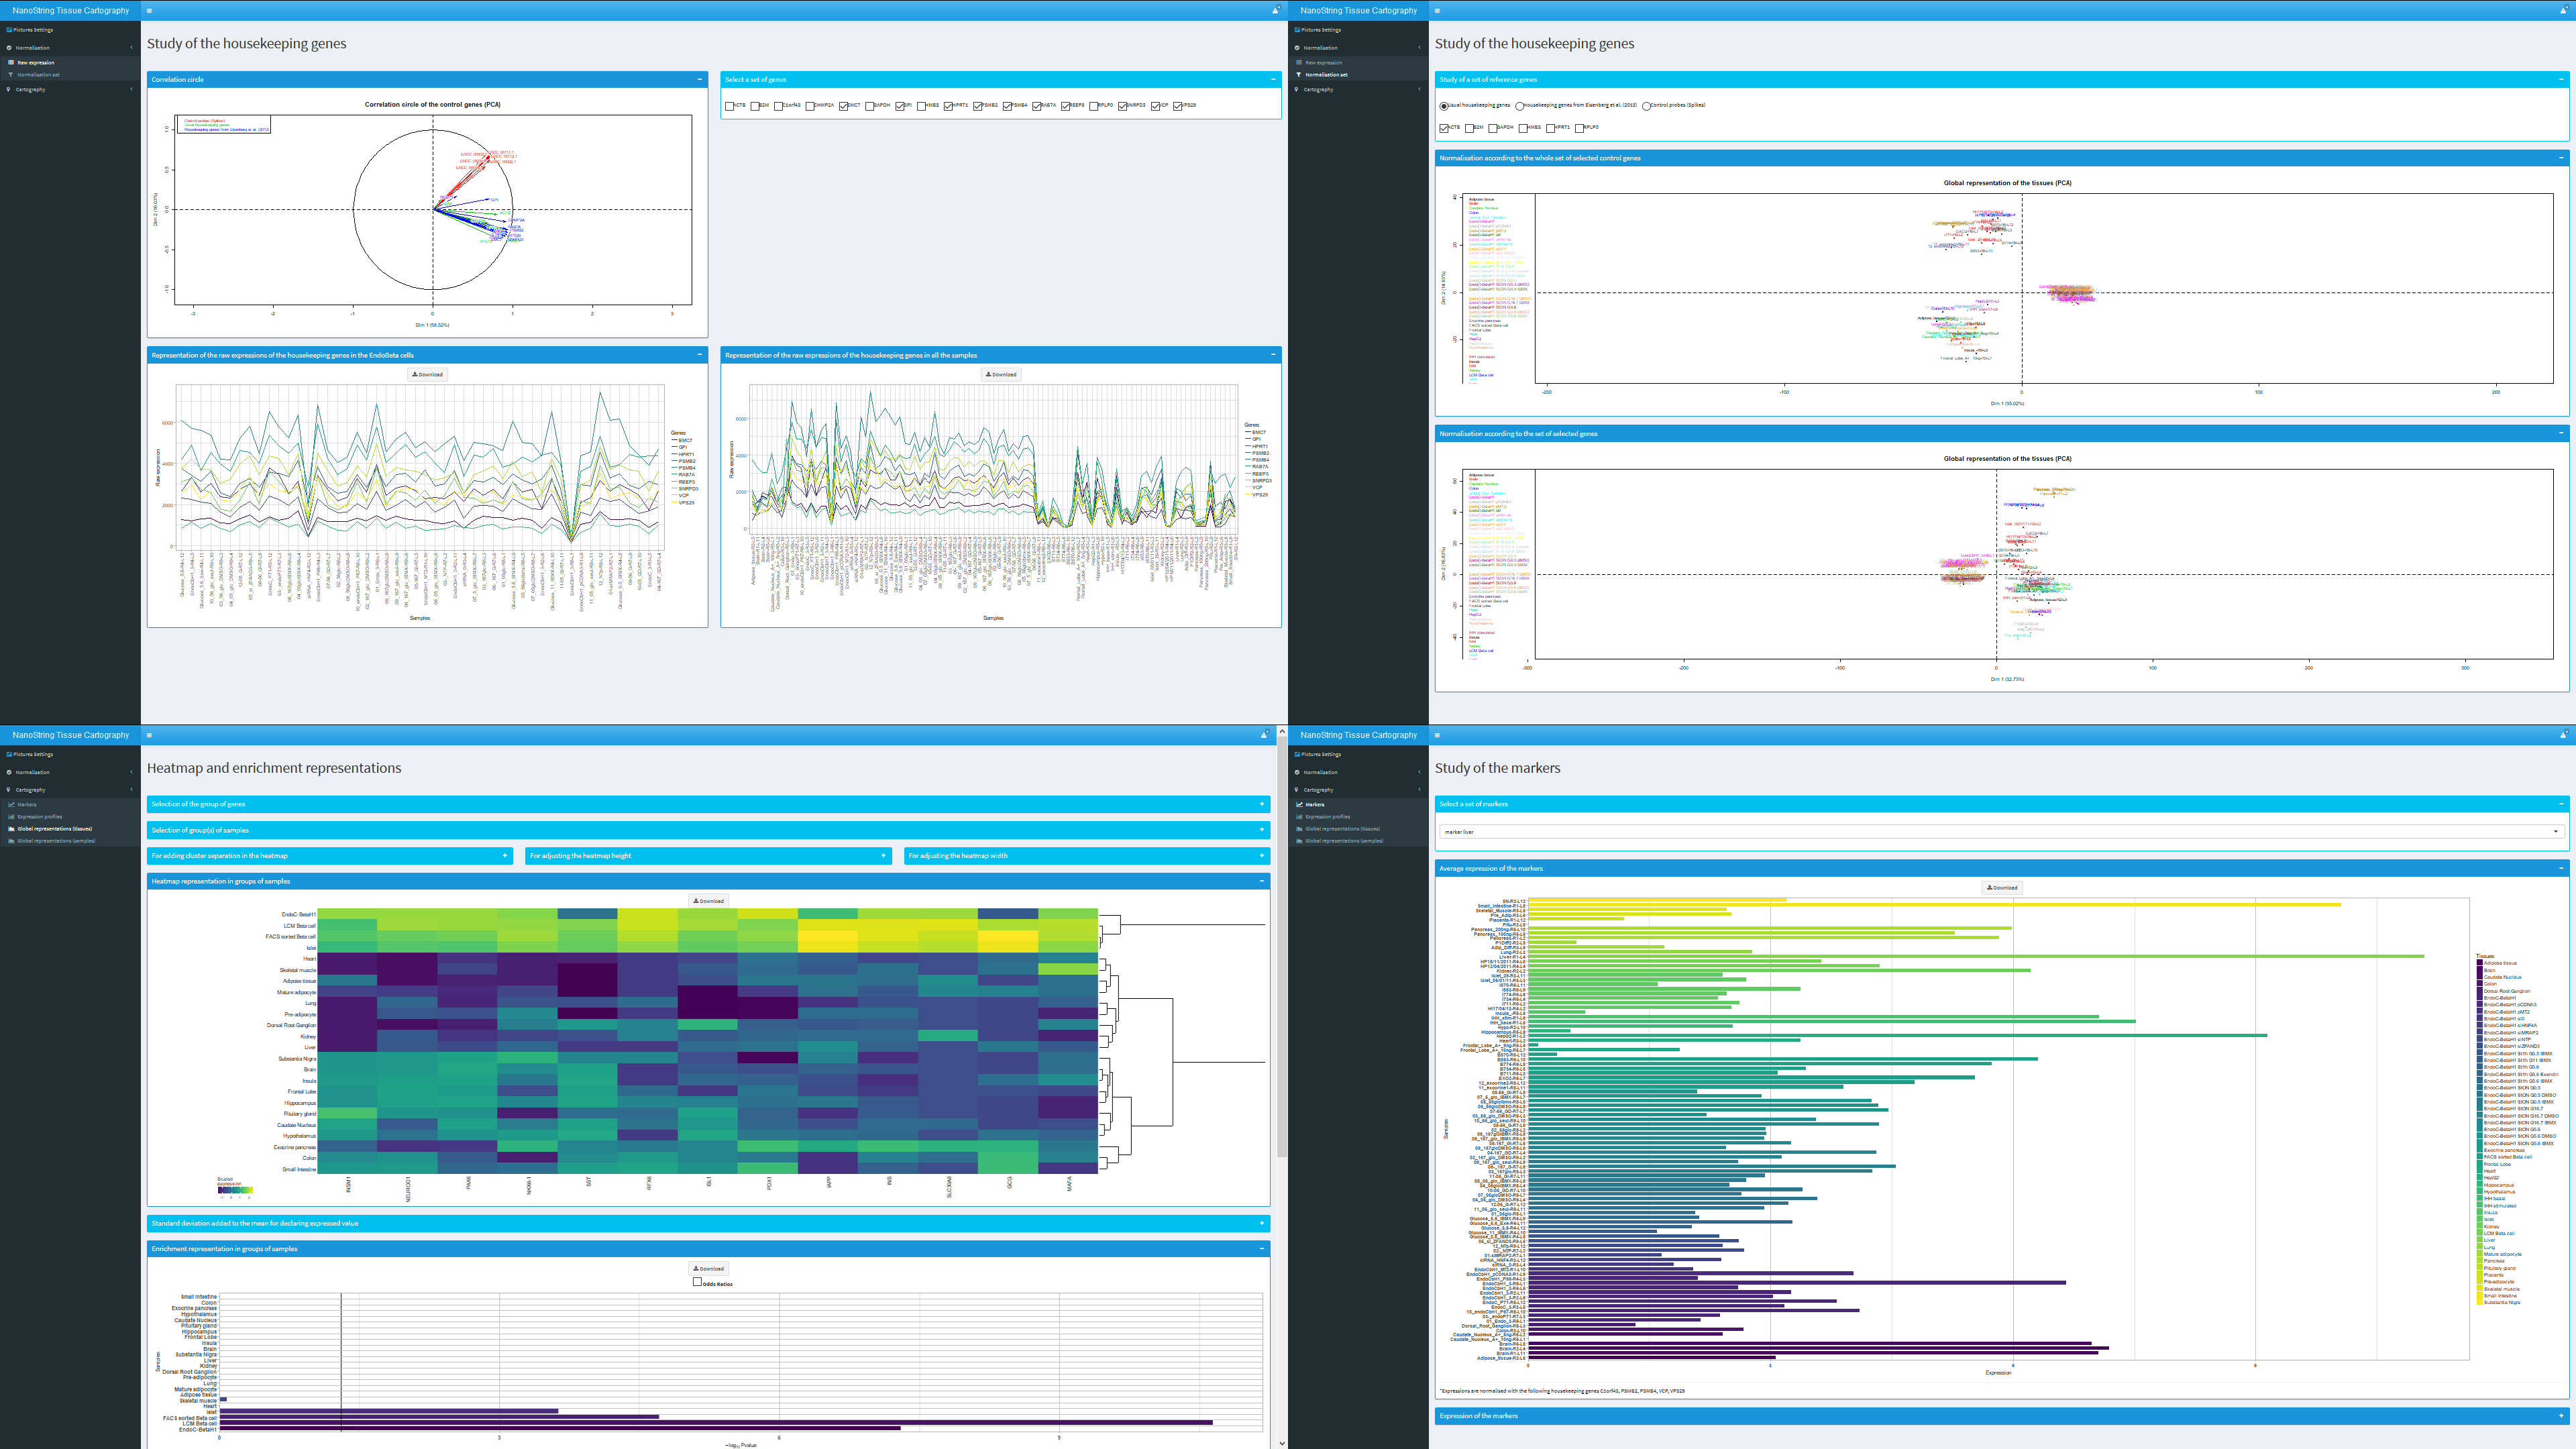
\includegraphics[width=6in]{FiguresTables/App2} 

}

\caption{Application Shiny développée dans le cadre de l'analyse de
l'expression de gènes de susceptibilité au diabète de type 2 dans un
panel pluritissulaire.}\label{fig:App2}
\end{figure}

Dans un premier temps, une interface web (Figure \ref{fig:App2}), via
l'extension R shiny \citep{R-shiny}, a été développée pour visualiser
l'ensemble des données générées, principalement à l'aide de
représentations ``heatmap'' et de dendrogrammes, créées à partir de la
classification hiérarchique des mesures d'expression (distance de Ward
sur les données centrées et réduites). Cette interface, permet la
visualisation et l'identification de groupes de gènes exprimés de façon
similaires entre les tissus, notamment dans les échantillons liés au
pancréas, siège de la sécrétion d'insuline. Dans un second temps, les
gènes ont été regroupés selon leur nature, à savoir les 104 gènes
candidats, les gènes spécifiques à chaque organe (p.~ex. gènes exprimés
uniquement dans le foie), et les gènes identifiés dans les formes
monogéniques de DT2. Pour chacun de ces ensembles, une table de
contingence a été construite sur la base des comptages de gènes
présentant une expression supérieure à celle observée en moyenne dans
l'ensemble des tissus
(\(Expr_{i}>\mu_{Tissus}+1,5\times\sigma_{Tissus}\)). L'enrichissement
en gènes surexprimés dans un ensemble et dans un tissu donné est testé
au moyen du test exact de Fisher. Les valeurs-p obtenues ont été
présentées sous la forme d'un histogramme au sein de l'interface web,
permettant la visualisation simultanée des résultats de l'enrichissement
des ensembles de gènes, ainsi que l'homogénéité ou l'hétérogénéité de
l'expression ces gènes.

\subsubsection{Sécrétion d'insuline en réponse au glucose (modèle
cellulaire)}\label{secretion-dinsuline-en-reponse-au-glucose-modele-cellulaire}

Le rôle des gènes candidats a été ensuite étudié en diminuant leur
expression au moyen de petits ARN interférents (siRNA), ayant pour
fonction de cibler spécifiquement les mRNA et induire leur dégradation,
dans un modèle de cellules \(\beta\) humaines (c.-à-d. EndoC
\(\beta H1\)).




\begin{figure}[!htb]

{\centering 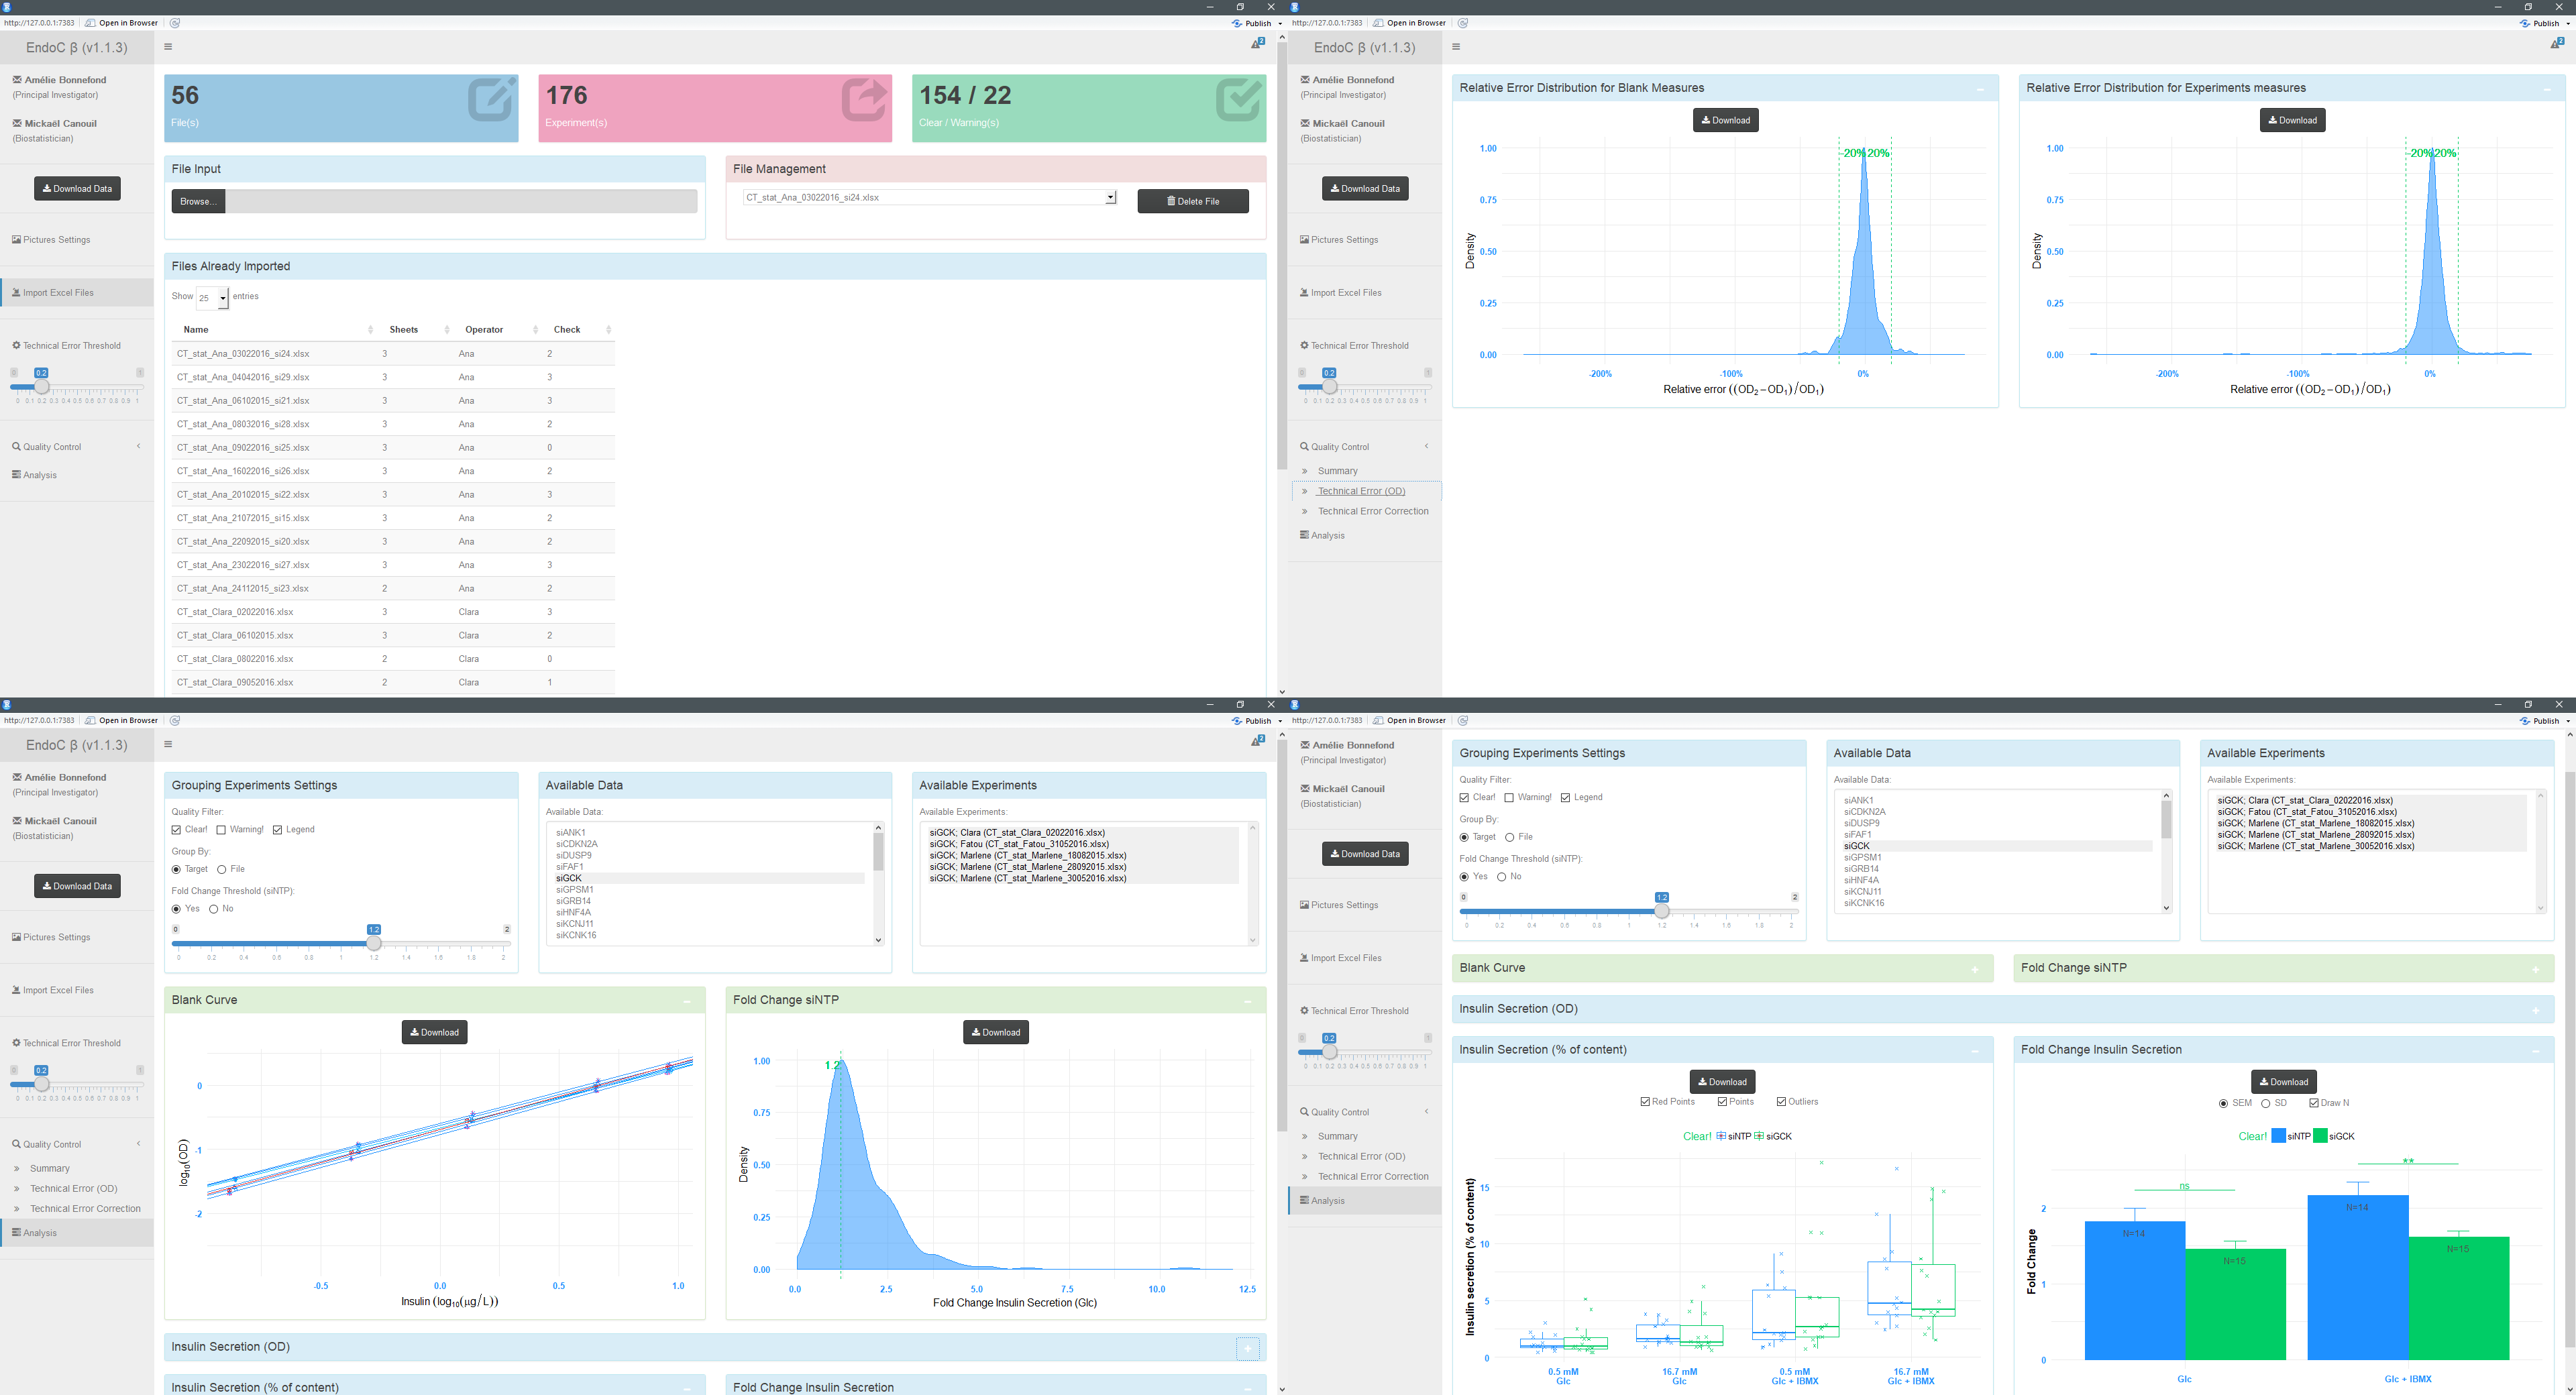
\includegraphics[width=6in]{FiguresTables/App1} 

}

\caption{Application Shiny développée dans le cadre de l'analyse de la
sécrétion d'insuline par le modèle cellulaire d'EndoC \(\beta\)H1.}\label{fig:App1}
\end{figure}

Le processus d'analyse comprend d'abord une étape de contrôle-qualité
des différentes étapes de l'expérimentation, notamment au niveau des
mesures de la gamme étalon d'absorbance, permettant d'évaluer la
sécrétion d'insuline par les cellules. Cette étape consiste en
l'évaluation du biais (erreur relative) entre les deux mesures
d'absorbance (duplicats) des triplicats expérimentaux (cellules), et des
mesures servant à établir la gamme étalon sur plus de 100 expériences.
Un seuil de qualité a été défini graphiquement via la courbe de
distribution des erreurs relatives des mesures d'absorbances~: les
expériences dont l'erreur relative était inférieure à 20~\% étaient
conservées pour analyse. Les expériences validant les critères du
contrôle-qualité sont ensuite analysées pour deux conditions de
stimulation~: glucose et glucose + IBMX (3-isobutyl-1-methylxanthine).
Les mesures de sécrétion d'insuline sont ainsi comparées entre les
cellules contrôles (où l'expression du gène n'est pas altérée), et les
cellules d'intérêt (où l'expression du gène est réduite via la
transfection d'un siRNA), par une approche de régression linéaire avec
ajustement sur les variables d'expérimentation, tels l'expérimentateur
et le jour de l'expérience. Les mesures de sécrétion d'insuline sont
ensuite exprimées en ``Fold Change''.

L'ensemble des étapes de contrôle-qualité et des analyses ont été
implémentées au sein d'une interface web (Figure \ref{fig:App1}), via
l'extension R shiny \citep{R-shiny} permettant la visualisation, à la
volée, de la qualité et des résultats de chaque expérience, dès leur
inclusion dans l'application.

\subsection{Résultats}\label{resultats-1}

\subsubsection{Spécificité et enrichissement dans un panel
pluritissulaire}\label{specificite-et-enrichissement-dans-un-panel-pluritissulaire-1}

L'étude transcriptomique des 104 gènes candidats a montré que ces gènes
étaient préférentiellement exprimés dans les cellules \(\beta\) du
pancréas~:

\begin{itemize}
\item
  cellules \(\beta\) prélevées à l'aide d'une microdissection par
  capture laser (LCM)~: \(\textrm{valeur-p}=5,1\times 10^{-4}\)
  (valeur-p du test exact de Fisher)~;
\item
  cellules \(\beta\) triées (``Fluorescence Activated Cell Sorting'' ou
  FACS)~: \(\textrm{valeur-p}=1,6\times 10^{-3}\)~;
\item
  modèle de cellules \(\beta\) (EndoC \(\beta H1\))~:
  \(\textrm{valeur-p}=1,6\times 10^{-3}\)~;
\end{itemize}

mais aucun enrichissement significatif de ces gènes n'a pu être montré
dans les tissus cibles de l'insuline (c.-à-d. foie, muscle squelettique
et tissu adipeux).

\subsubsection{Sécrétion d'insuline en réponse au glucose (modèle
cellulaire)}\label{secretion-dinsuline-en-reponse-au-glucose-modele-cellulaire-1}

L'étude de la sécrétion de l'insuline par les EndoC \(\beta H1\), pour
les gènes dont la transfection de siRNA a réussi, a permis
l'identification et la confirmation de sept gènes (\emph{GCK},
\emph{HNF4A}, \emph{TCF19}, \emph{SLC30A8}, \emph{TBC1D4}, \emph{CDKN2A}
et \emph{KNCK16}) connus pour être exprimés ou ayant un rôle dans les
cellules \(\beta\), et particulièrement sur la sécrétion d'insuline.
L'approche développée ici a également permis de mettre en lumière quatre
gènes candidats additionnels (\emph{PRC1}, \emph{SRR}, \emph{ZFAND3} et
\emph{ZFAND6}), pouvant impacter la sécrétion d'insuline, et dont le
rôle dans la cellule \(\beta\) en fait de bons candidats pour l'étude
des mécanismes liant la cellule \(\beta\) au développement d'un diabète
de type 2. L'expression de ces gènes a été validée par
immunofluorescence. De plus, une corrélation positive significative a
été retrouvée dans les ilots de cellules \(\beta\) pancréatiques de
souris entre l'expression de l'insuline et l'expression de ces quatre
gènes. Enfin, un séquençage de l'ARN d'EndoC \(\beta H1\), transfectées
avec \emph{siPRC1}, \emph{siSRR}, \emph{siZFAND6}, \emph{siZFAND3} ou
\emph{siNTP} (contrôle), a été réalisé afin d'identifier des voies
physiopathologiques pouvant expliquer la corrélation avec la sécrétion
d'insuline observée (p.~ex. réseau de gènes liés à l'apoptose des
cellules \(\beta\) pancréatiques, au stress du reticulum endoplasmique,
etc.)

\subsection{Conclusion}\label{conclusion-1}

Les développements statistiques apportés dans cette étude fonctionnelle,
quoique non directement appliquée à l'ensemble des gènes localisés au
voisinage des SNPs identifiés par GWAS ou méta-analyses, se révèlent des
outils robustes ayant permis de mettre en évidence un aspect plus
mécanistique/pathophysiologique des loci identifiés par les approches
GWAS, augmentant ainsi la compréhension des maladies complexes.

\section{Article}\label{article-1}

Article disponible en ligne sur \textbf{\emph{Molecular Metabolism}}
(\url{http://doi.org/10.1016/j.molmet.2017.03.011}) \clearpage

\chapter{La Surexpression Hépatique de PDGF-AA Affaiblit la
Signalisation de l'Insuline dans le Diabète}\label{Article3}

\chaptermark{La Surexpression Hépatique de PDGF-AA Affaiblit la Signalisation de l'Insuline dans le Diabète}
Soumis à \textbf{\emph{Nature Communications}}.

Amar Abderrahmani\textsuperscript{1,2\textasteriskcentered}, Loïc
Yengo\textsuperscript{1\textasteriskcentered}, Robert
Caiazzo\textsuperscript{3\textasteriskcentered}, \textbf{Mickaël
Canouil\textsuperscript{1\textasteriskcentered}}, Stéphane
Cauchi\textsuperscript{1}, Violeta Raverdy\textsuperscript{2}, Valérie
Plaisance\textsuperscript{1}, Stéphane Lobbens\textsuperscript{1}, Julie
Maillet\textsuperscript{1}, Laure Rolland\textsuperscript{1}, Raphael
Boutry\textsuperscript{1}, Maxime Kwapich\textsuperscript{1}, Mathie
Tenenbaum\textsuperscript{1}, Julien Bricambert\textsuperscript{1},
Sophie Saussenthaler\textsuperscript{4}, Elodie
Anthony\textsuperscript{5}, Pooja Jha\textsuperscript{6}, Julien
Derop\textsuperscript{1}, Olivier Sand\textsuperscript{1}, Iandry
Rabearivelo\textsuperscript{1}, Audrey Leloire\textsuperscript{1}, Marie
Pigeyre\textsuperscript{2}, Martine Daujat-Chavanieu\textsuperscript{7},
Sabine Gerbal-Chaloin\textsuperscript{7}, Tasnim
Dayeh\textsuperscript{8}, Guillaume Lassailly\textsuperscript{2},
Philippe Mathurin\textsuperscript{9}, Bart Staels\textsuperscript{10},
Johan Auwerx\textsuperscript{5}, Annette Schürmann\textsuperscript{4},
Catherine Postic\textsuperscript{5}, Clemens
Schafmayer\textsuperscript{11}, Jochen Hampe\textsuperscript{12}, Amélie
Bonnefond\textsuperscript{1,2}, François
Pattou\textsuperscript{3\textdagger} \& Philippe
Froguel\textsuperscript{1,2\textdagger}

\footnotesize
\textsuperscript{1}Univ. Lille, CNRS, Institut Pasteur de Lille, UMR
8199 - EGID, F-59000 Lille, France~; \textsuperscript{2}Department of
genomics of common disease, Imperial College London, UK~;
\textsuperscript{3}Univ. Lille, Inserm, CHU Lille, U1190 - EGID, F-59000
Lille, France~; \textsuperscript{4}Department of Experimental
Diabetology, German Institute of Human Nutrition Potsdam-Rehbrüecke,
Nuthetal and German Center for Diabetes Research (DZD),
München-Neuherberg, Germany~; \textsuperscript{5}Inserm, U1016, Institut
Cochin, Paris, France CNRS UMR 8104, Paris, France Université Paris
Descartes, Sorbonne Paris Cité, Paris, France~;
\textsuperscript{6}Laboratory of Integrative and Systems Physiology,
École Polytechnique Fédérale de Lausanne, 1015 Lausanne, Switzerland~;
\textsuperscript{7}INSERM U1183, Univ. Montpellier, UMR 1183, Institute
for Regenerative Medicine and Biotherapy, CHU Montpellier, France~;
\textsuperscript{8}Department of clinical science~; Skane University
Hospital Malmö, Malmö, Sweden~; \textsuperscript{9}Univ. Lille, Inserm,
CHU Lille, U995 - LIRIC - Lille Inflammation Research International
Center, F-59000 Lille, France~; \textsuperscript{10}Univ. Lille, Inserm,
CHU Lille, Institut Pasteur de Lille, U1011- EGID, F-59000 Lille,
France~; \textsuperscript{11}Department of Visceral and Thoracic
Surgery, University Hospital Schleswig-Holstein, Kiel, Germany~;
\textsuperscript{12}Medical Department 1, Technische Universität Dresden
(TU Dresden), Dresden, Germany.

\textsuperscript{\textasteriskcentered}Co-premier auteurs.\\
\textsuperscript{\textdagger}Co-dernier auteurs. \normalsize

\clearpage

\section{Introduction}\label{introduction-3}

\subsection{Contexte/objectifs}\label{contexteobjectifs-2}

Les études d'association pangénomique (GWAS) n'ont pu expliquer
qu'environ 15~\% de l'héritabilité du diabète de type 2 (DT2). Les
mécanismes sous-jacents à la pathophysiologie du DT2 et aux
complications dérivées de celui-ci, comme les stéatoses hépatiques
non-alcooliques (NAFLD~: ``Non-Alcoholic Fatty Liver Disease''~; NASH :
``Non-Alcoholic SteatoHepatitis''), restent en grande partie méconnus.
Les modifications épigénétiques de l'ADN dans un tissu clé tel que le
foie pourraient contribuer à expliquer une partie de cette héritabilité
manquante dans le DT2 et/ou fournir des indications sur le lien entre le
DT2 et ses complications. Une étude du méthylome et du transcriptome du
foie de patientes obèses a été réalisée selon une approche cas/témoins
(96 DT2 contre 96 normoglycémiques).

\subsection{Méthodes}\label{methodes-2}

\subsubsection{Génome}\label{genome-1}

Le génotypage des 192 individus provenant de la cohorte ABOS (Atlas
Biologique de l'Obésité Sévère), a été réalisé au moyen de la puce
Illumina Metabochip, une puce personnalisée comportant 200~000 SNPs,
dont environ 120~000 situés près de 257 loci identifiés par GWAS pour
plusieurs traits comme le diabète de type 2 ou la glycémie. Ces données
de génotypage ont fait l'objet d'un contrôle-qualité visant à exclure
les SNPs dont le taux de génotypage était inférieur à 95~\% et dont
l'équilibre de Hardy-Weinberg n'était pas respecté
(\(\textrm{valeur-p}<=10^{-4}\)). Afin de vérifier l'homogénéité
ethnique de nos indivius, une analyse en composantes principales a été
réalisée sur un jeu de données combinant les génotypes (196~470 SNPs)
des 192 individus, aux génotypes de 272 individus provenant du projet de
génotypage HapMap comportant 87 individus caucasiens (Europe de l'ouest
et du nord), 97 individus asiatiques (Chine, Beijing) et 88 individus
africains (Nigéria). À partir des SNPs précédemment identifiés par GWAS
(disponibles sur la puce Illumina Metabochip) comme étant associés à
l'insulinémie à jeun (19 SNPs), à la glycémie à jeun (24 SNPs), au
risque de DT2 (65 SNPs) et à l'indice de masse corporelle (97 SNPs),
quatre scores de risque génétique (GRS) ont été construits en prenant la
somme des allèles à risque portés par chaque individu.

\subsubsection{Méthylome}\label{methylome}

L'ensemble des sites de méthylation disponibles au sein de la puce
Illumina HumanMethylation450 ont été analysés dans l'objectif
d'identifier des marques de méthylation associées au statut diabétique
des individus. Une étape de contrôle-qualité des données brutes (format
IDAT) a été réalisée sur la base de deux critères~:

\begin{itemize}
\item
  exclusion des individus avec moins de 75~\% des sites de méthylation
  détectés (\(\textrm{valeur-p}<10^{-16}\)) selon le logiciel Illumina
  GenomeStudio (outil permettant la lecture des images de
  fluorescence)~;
\item
  exclusion des sites de méthylation lorsque le niveau de méthylation
  n'a pu être détecté (\(\textrm{valeur-p}<10^{-16}\)) dans au moins
  95~\% des individus, selon le logiciel Illumina GenomeStudio.
\end{itemize}

Suite à l'application de ces critères, l'ensemble des individus et
environ 85~\% (416~693) des sites de méthylation ont été conservés pour
analyse.

La puce Illumina HumanMethylation450 comporte deux technologies de
détection des niveaux de méthylation (valeur-\(\beta\))~: sondes
Infinium I et sondes Infinium II. Une étape de normalisation est
effectuée, d'une part, pour corriger un éventuel effet plaque, et
d'autre part, pour corriger les différences de méthylation entre les
deux types de sondes, en particulier au niveau de la distribution des
niveaux de méthylation. La méthode BMIQ (``Beta-MIxture Quantile
normalisation'') a permis de normaliser la distribution des
valeurs-\(\beta\) des sondes Infinium II par rapport à celles des sondes
Infinium I, tout en conservant la variabilité biologique inhérente aux
différentes sondes (p.~ex. Infinium I principalement employée pour les
îlots CpG tandis que Infinium II est employée pour des sites CpG
isolés), ainsi que le caractère monotone (rang) des valeurs-\(\beta\)
pour chaque type de sonde. Cette méthode consiste à modéliser la
distribution des valeurs-\(\beta\) (Infinium II) sur la base de trois
états de méthylation, soit méthylé, semi-méthylé et non-méthylé, dont
les paramètres sont estimés au moyen d'un algorithme EM
(Espérance-Maximisation). Une transformation quantile des
valeurs-\(\beta\) (Infinium II) est ensuite appliquée sur la base de la
distribution estimée. Une analyse en composantes principales est
réalisée sur l'ensemble des données afin d'identifier une potentielle
structure (p.~ex. plusieurs sous-populations) et de potentiels individus
extrêmes en termes de profil de méthylation.

Les sites différentiellement méthylés, selon le statut diabétique, ont
été identifiés au moyen d'une régression linéaire avec un ajustement sur
le niveau de stéatose (en pourcentage), la NASH (trait binaire) et la
fibrose (trait binaire) en plus des covariables classiques tels l'âge et
l'indice de masse corporelle (IMC). Les valeurs-p sont ensuite corrigées
par un facteur d'inflation selon la méthode du ``contrôle génomique''
utilisée dans les GWAS pour corriger des effets liés à une éventuelle
stratification du groupe cas et du groupe témoin menant à une inflation
de l'erreur de type 1. Enfin, une correction de Bonferroni pour tests
multiples est appliquée, produisant un seuil de significativité nominal
\(10^{-7}\).

\subsubsection{Transcriptome}\label{transcriptome-1}

Le transcriptome a été étudié sur l'ensemble des individus via la puce
Illumina HumanHT-12 v4, qui permet de mesurer l'ARN sur plus de 47~000
sondes, dont moins de 4~000 correspondant à de l'ARN non-codant. Après
lecture de la fluorescence et attribution d'une valeur-p par le logiciel
Illumina GenomeStudio, les données provenant de deux expérimentations
font l'objet d'une normalisation quantile pour corriger les différences
de distribution entre les mesures d'expression des deux séries de puces.
Les sondes d'expression ne présentant pas une valeur-p de détection
inférieure à \(\alpha = 0,05\) pour l'ensemble des individus étaient
exclues, aboutissant à 18~412 sondes (13~664 gènes) et 189 individus
conservés pour les analyses. À cela s'ajoute l'exclusion de deux
individus présentant des profils transcriptomiques extrêmes, et détectés
au moyen d'une analyse en composantes principales. L'expression
différentielle selon le statut DT2 a été testée par une approche de
régression linéaire avec ajustement pour l'âge et l'IMC, et dont la
significativité a été évaluée sur la base d'un seuil FDR (``False
Discovery Rate'') à 5~\%.

\subsection{Résultats}\label{resultats-2}

\subsubsection{Diabète de type 2}\label{diabete-de-type-2}

Après correction des valeurs-p, le site CpG cg14496282 localisé sur le
gène \emph{PDGFA} (``Platelet-Derived Growth Factor subunit A'') a été
mis en évidence comme associé significativement au risque de DT2
(\(\beta = -15,6 \%\)~; \(\textrm{valeur-p}=2,5\times 10^{-8}\)), avec
une hypométhylation chez les DT2 (\(41,3\)~\% en moyenne) et une
hyperméthylation chez les témoins (\(60,3\)~\% en moyenne). Cette
association persiste lorsqu'on ajuste sur la composition cellulaire du
tissu (\(\beta = -14,9 \%\)~; \(\textrm{valeur-p}=6,9\times 10^{-7}\)),
celle-ci étant évaluée au moyen d'une méthode d'estimation de la
contribution au méthylome global, d'un nombre donné de types cellulaires
déterminés selon une approche ``Bootstrap'' (méthode de
rééchantillonnage). De plus, une étude de réplication dans une cohorte
allemande comportant 12 cas et 53 témoins, a montré des résultats
cohérents avec notre étude (\(\beta = -14 \%\)~;
\(\textrm{valeur-p}=0,01\)). L'étude de l'expression du gène
\emph{PDGFA} démontre que celle-ci est inversement corrélée au niveau de
méthylation du site cg14496282. La méthylation du site cg14496282 a
également été montrée dans notre étude (dans le groupe témoin) comme
étant associée à une diminution de l'insulinémie à jeun et de
l'insulinorésistance (indice HOMA2-IR), pendant que l'expression de
\emph{PDGFA} était associée à une augmentation de l'insuline à jeun et
une diminution de l'insulinorésistance.

\subsubsection{Complication~:
stéatose/fibrose}\label{complication-steatosefibrose}

La méthylation de cg14496282 a également été montrée comme étant
associée à une diminution du risque de NASH C chez les individus
diabétiques et les individus normoglycémiques, alors que la méthylation
était associée à une diminution de fibrose hépatique, et l'expression à
une augmentation de fibrose hépatique chez les DT2. Ces résultats sont
cohérents avec des études ayant précédemment montré que l'activation du
récepteur PDGF stimule les cellules stellaires et accroît ainsi la
fibrose du foie. De plus, il a été montré que la surexpression de
\emph{Pdgfa} dans le foie de souris engendre une fibrose spontanée du
foie.

\subsubsection{\texorpdfstring{\emph{PDGFA} et action de
l'insuline}{PDGFA et action de l'insuline}}\label{pdgfa-et-action-de-linsuline}

L'association négative entre le GRS associé à l'insulinémie et la
méthylation de cg14496282 (\(1,05 \%\)~;
\(\textrm{valeur-p}=4\times 10^{-3}\)), demeurant robuste aux
ajustements à l'IMC, au cholestérol (HDL) ou aux triglycérides, suggère
que l'hyperinsulinémie contribue à la modification (diminution) du
niveau de méthylation du site cg14496282 de \emph{PDGFA}. Dans le même
temps, aucune association entre la méthylation de cg14496282 et les GRS
associés à la glycémie à jeun, le statut DT2 et l'obésité (IMC), n'a été
observée dans notre étude. La relation entre l'expression de
\emph{PDGFA} et la méthylation de cg14496282 dans des conditions
hyperinsulinémiques a également été vérifiée \emph{in vitro} (c.-à-d.
avec des hépatocytes primaires humains et des hépatocytes humains
immortalisés). Un modèle murin a permis l'étude de l'expression de
\emph{Pdgfa}, qui était augmentée sous stimulation insuline. Cependant,
la méthylation de cg14496282 n'a pu être étudiée dans ce dernier modèle,
puisque le site n'est pas conservé entre l'Homme et la souris.

\subsection{Conclusion}\label{conclusion-2}

La contribution de l'épigénétique dans la pathophysiologie du DT2,
notamment dans la dérégulation des fonctions du foie, reste compliquée à
appréhender mais fournit tout de même de nouvelles pistes
d'investigation. En effet, l'étude \emph{in vitro} et \emph{in vivo}, en
plus de l'étude génétique au moyen des GRS dans notre étude, nous
indique que l'hyperinsulinémie pourrait avoir un effet causal sur la
méthylation de cg14496282 et sur l'expression de \emph{PDGFA}. De plus,
notre étude fonctionnelle suggère que \emph{PDGFA} pourrait avoir un
effet autocrine sur l'hyperinsulinémie, c'est-à-dire parallélement à la
stimulation de l'expression de \emph{PDGFA} par la voie de l'insuline,
l'expression de \emph{PDFGA} induit la sécrétion d'insuline via
l'activation de PKC (Protéine Kinase C).

Les associations de \emph{PDFGA} et des altérations du foie (plus
précisément, fibrose et stéatose) trouvées dans plusieurs études et la
nôtre soutiennent l'hypothèse du rôle fibrotique de \emph{PDFGA} dans le
foie au moyen d'une élévation de l'insulinémie. En outre, les études
fonctionnelles réalisées sur des modèles cellulaires, incluant l'étude
de la metformine (traitement principal utilisé dans le diabète de type
2), soulignent la portée de nos découvertes, en particulier, en tant que
cible thérapeutique du DT2 et de ses complications. L'étude du méthylome
se révèle être un outil efficace dans l'étude de la pathogenèse des
maladies communes, particulièrement lorsqu'elle cible un type cellulaire
ou un tissu spécifique.

\section{Article}\label{article-2}

\clearpage

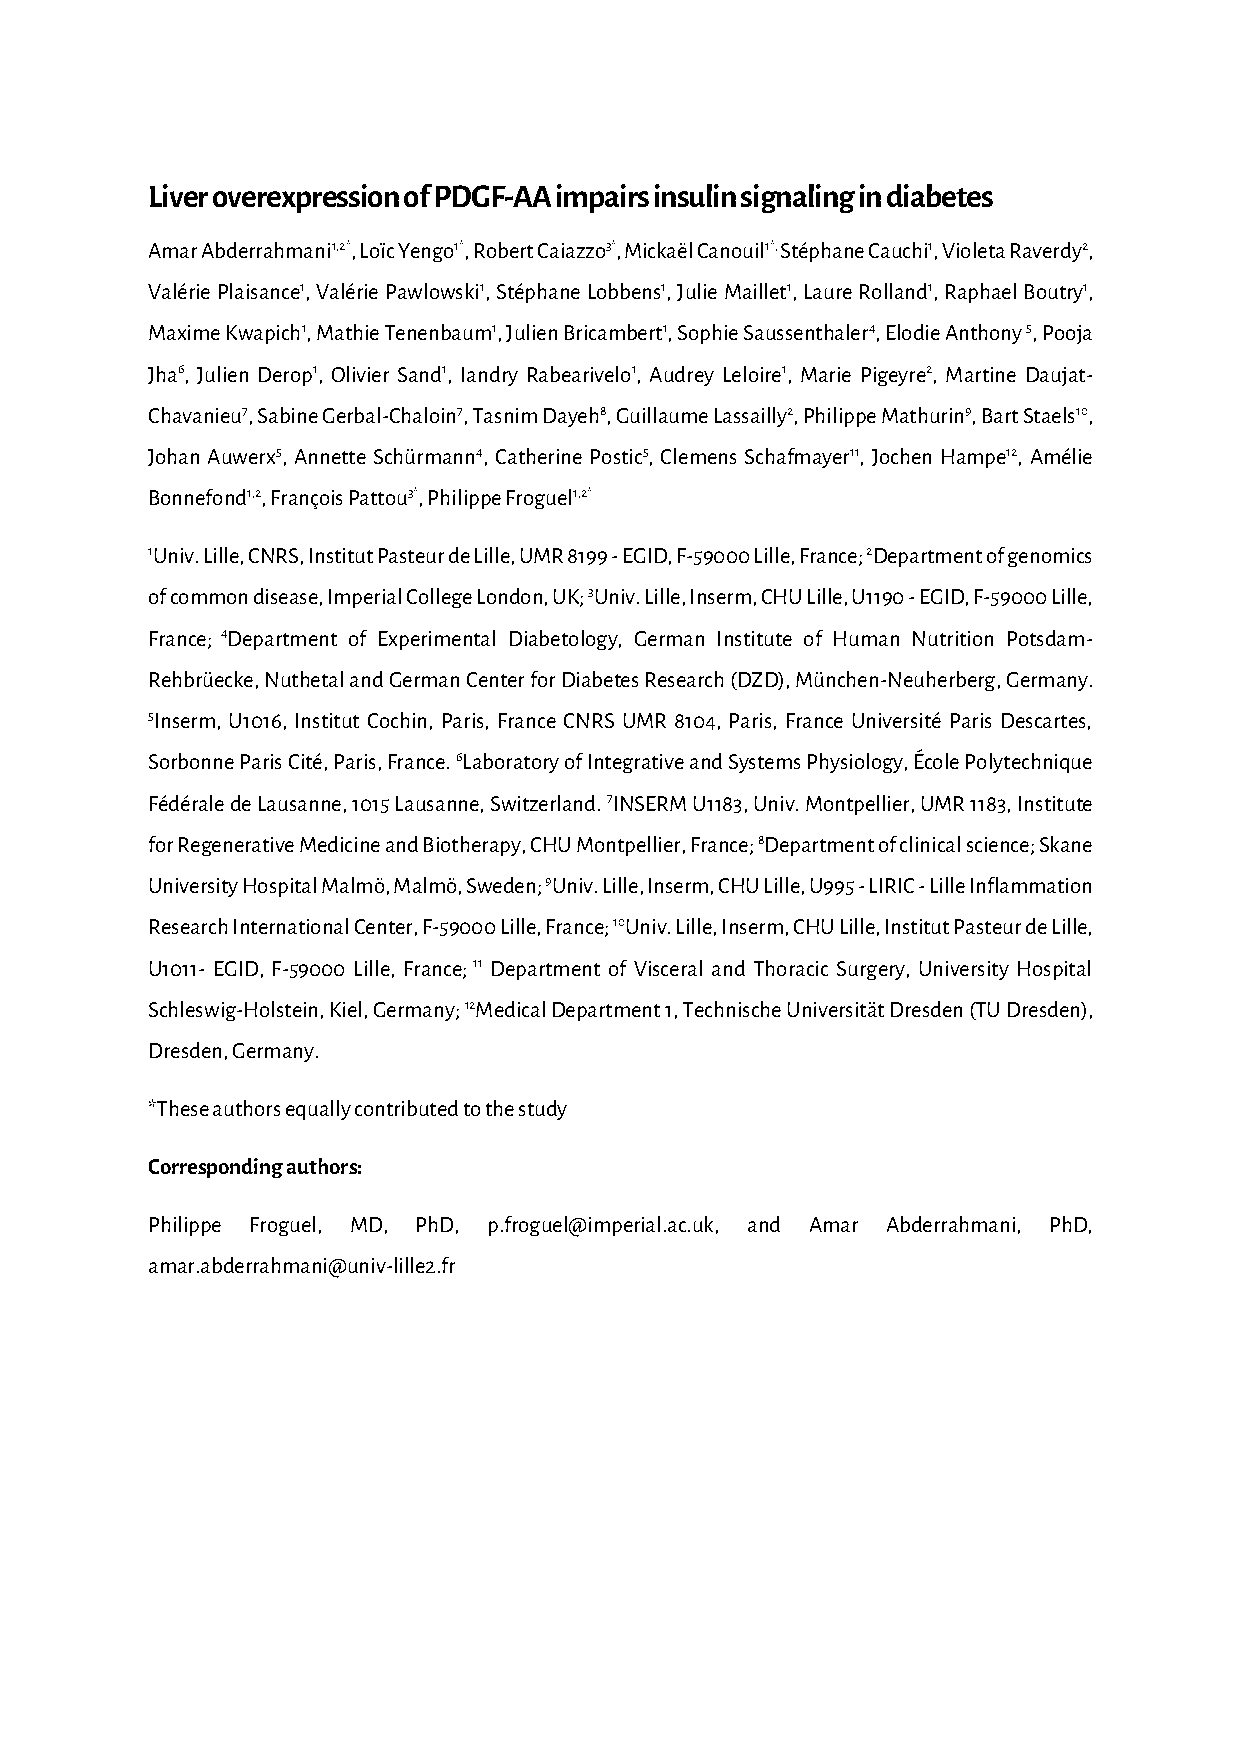
\includepdf[pages=-, scale=1, clip, fitpaper=true, offset = 0cm -0.3cm, pagecommand={\thispagestyle{headings}}]{Articles/Article3.pdf}
\includepdf[pages=35-47, scale=0.8, clip, trim=0cm 0cm 0cm 0cm, pagecommand={\thispagestyle{headings}}]{Articles/Article3_Figures.pdf}

\chapter{L'Exposition à Faible Dose aux Bisphénols A, F et S des
Adipocytes Primaires Humains Modifie les Profils d'ARN Codant et
Non-Codant}\label{Article4}

\chaptermark{L'Exposition à Faible-Dose, aux Bisphénols A, F et S, des Adipocytes Primaires Humain [...]}
Publié dans
\textbf{\emph{\href{http://doi.org/10.1371/journal.pone.0179583}{PLoS ONE}}}.

Marie Verbanck\textsuperscript{1,\textasteriskcentered}, \textbf{Mickaël
Canouil\textsuperscript{1,\textasteriskcentered}}, Audrey
Leloire\textsuperscript{1}, Véronique Dhennin\textsuperscript{1}, Xavier
Coumoul\textsuperscript{2}, Loïc Yengo\textsuperscript{1}, Philippe
Froguel\textsuperscript{1,3,\textdagger} \& Odile
Poulain-Godefroy\textsuperscript{1,\textdagger}

\footnotesize
\textsuperscript{1}Univ. Lille, CNRS, CHU Lille, Institut Pasteur de
Lille, UMR 8199 - EGID, F-59000 Lille, France~;
\textsuperscript{2}INSERM UMR-S 1124, Toxicologie Pharmacologie et
Signalisation cellulaire, 75006 Paris, France~; Université Paris
Descartes, ComUE Sorbonne Paris Cité, 75006 Paris, France~;
\textsuperscript{3}Department of Genomics of Common Disease, School of
Public Health, Imperial College London, United Kingdom.

\textsuperscript{\textasteriskcentered}Co-premier auteurs.\\
\textsuperscript{\textdagger}Co-dernier auteurs. \normalsize

\clearpage

\section{Introduction}\label{introduction-4}

\subsection{Contexte/objectifs}\label{contexteobjectifs-3}

L'exposition des populations au bisphénol A (BPA) a été suspectée de
participer à l'épidémie d'obésité et de désordres métaboliques. Le BPA,
avant son interdiction en Europe et notamment en France, était utilisé
dans la fabrication de plastiques et de résines époxy, et couramment
utilisé dans les contenants alimentaires tels que les biberons ou les
revêtements de protection des boîtes de conserve. Le BPA se retrouve
également dans certains jouets, appareils médicaux et certains papiers
comme les tickets de caisse. Depuis l'interdiction de l'usage du BPA,
des composés analogues ont vu le jour, tels que le bisphénol S (BPS) et
le bisphénol F (BPF), et sont maintenant utilisés de façon courante. À
ce jour, les études toxicologiques portant sur les BPS et BPF sont peu
nombreuses.

Notre hypothèse est que les substituts du BPA pourraient avoir un effet
similaire à celui du BPA, notamment au niveau du tissu adipeux. À cet
effet, nous avons comparé le profil d'expression des ARN codants et
non-codants d'adipocytes primaires humains exposés à ces différents
bisphénols au cours de leur différenciation.

\subsection{Méthodes}\label{methodes-3}

Les adipocytes primaires provenant de trois patientes caucasiennes et
non diabétiques ont été cultivés en présence des différents bisphénols
(BPA, BPS et BPF) à deux concentrations différentes~: 10 nM,
correspondant à la concentration de BPA observée dans les fluides
corporels de la population générale, et 10 µM, pour mesurer un potentiel
effet de concentration. Une condition contrôle, correspondant au tampon
utilisé pour diluer les différents bisphénols (DMSO) lors de la culture
et de la différenciation des adipocytes primaires, a été utilisée pour
fins de comparaison. Après différenciation des adipocytes primaires en
adipocytes, l'ARN a été extrait et les profils ARN ont été évalués via
une puce Agilent SurePrint G3 Human V2 pour les mRNA et lncRNA, et via
une puce Agilent SurePrint G3 miRNA pour les miRNA. L'ARN d'adipocyte
primaire (non différencié) a également été extrait pour évaluation du
statut de différenciation des cellules. En effet, certains gènes ne sont
exprimés que dans les adipocytes différenciés.

Un contrôle-qualité des données générées par ces deux plateformes a
ensuite été réalisé. Un premier filtre des sondes de mRNA/lncRNA est
appliqué pour exclure les sondes n'étant pas exprimées. Les valeurs
d'expression ont été considérées comme manquantes (car mal détectées ou
non exprimées) lorsque la valeur-p de détection, telle que fournie par
le logiciel d'analyse d'Agilent, était non-significative
(\(\textrm{valeur-p}>0,05\)). Les sondes dont le taux de valeurs
manquantes était inférieur à 5~\% étaient conservées pour analyse
(c.-à-d. les sondes exprimées dans au moins 95~\% des échantillons). Les
données ont ensuite été normalisées via une normalisation quantile
implémentée dans les extensions R \emph{limma} et \emph{AgiMicroRna},
pour corriger un ``effet plaque'' résultant de l'utilisation de
plusieurs puces. Afin de limiter l'impact de cet éventuel ``effet
plaque'', les différentes conditions expérimentales ont été réparties
sur les différentes puces selon un plan factoriel. À cette étape de
correction de l'effet plaque s'ajoute une normalisation de l'expression
des gènes à partir de gènes de ménage (gènes ubiquitaires dont le niveau
d'expression est constant dans l'ensemble des tissus), afin de rendre
l'expression des gènes d'intérêt comparable, en forçant l'expression des
gènes de ménage à être constante (p.~ex. égal à 1 dans le cas de
l'utilisation du ratio \(\frac{G_{cible}}{G_{ménage}}\), ou de façon
équivalente, égal à 0 après transformation logarithmique). Une analyse
en composantes principales a été réalisée sur l'ensemble des sondes
passant le contrôle-qualité pour les données de mRNA/lncRNA et miRNA
dans le but d'identifier une structuration des données associée au
statut de différenciation des adipocytes primaires ou aux différents
patients.

Pour chacun des trois patients, 4 échantillons contrôles (DMSO~:
contrôle négatif), 2 échantillons pour chaque combinaison de bisphénols
(BPA, BPS, BPF) et de concentrations (10 nM et 10 µM) ont produit
globalement \(4 + 2\times(3\times2) = 16\) échantillons par patient. Les
sondes mRNA, lncRNA et miRNA différentiellement exprimées ont été
identifiées à l'aide d'un modèle linéaire mixte, pour un bisphénol
donné, avec en effet fixe la concentration de bisphénol (10 nM et/ou 10
µM) comparée à la condition contrôle (DMSO), et avec effet aléatoire le
patient. L'analyse portant sur plus de 22~000 sondes mRNA/lncRNA et 483
sondes miRNA, une correction pour tests multiples a été appliquée pour
déterminer la significativité des effets selon la méthode de Benjamini
et Hochberg au seuil de 5~\%. Pour visualiser efficacement les
similarités et dissimilarités des différentes sondes entre les
conditions analysées, une représentation en ``heatmap'' a été utilisée.

\subsection{Résultats}\label{resultats-3}

Les analyses ont permis de mettre en évidence un ensemble de 846 sondes
mRNA/lncRNA dont l'expression était réduite en présence d'un bisphénol
(BPA, BPF et BPS) dans une concentration ``physiologique'' de 10 nM et
de 417 sondes dont l'expression était augmentée par rapport à la
condition contrôle (DMSO). Avec une concentration ``forte'' de 10 µM
lors de différenciation des adipocytes primaires, nous avons pu
identifier 774 et 1~106 sondes présentant, respectivement, une
diminution et une augmentation de l'expression en présence de
bisphénols. Certaines de ces dérégulations dans l'expression de ces
sondes, associées à la présence de bisphénols dans le milieu de culture
pendant la différenciation, sont partagées entre les BPA, BPF et BPS,
mais aussi entre les deux concentrations (10 nM et 10 µM). Des résultats
similaires ont également pu être observés pour l'ARN non codant (miRNA).

L'utilisation de l'outil IPA (\emph{Ingenuity Pathway Analysis}) a
permis d'identifier des voies/fonctions biologiques/métaboliques
présentant un enrichissement des sondes identifiées dans ces voies. Les
dérégulations associées à la présence de bisphénols pourraient être
impliquées dans les voies liées au ``cancer'' et à des ``anomalies et
blessures de l'organisme''. IPA a permis également d'analyser les
régulateurs en amont des dix gènes dérégulés communs pour les trois
bisphénols et les deux concentrations. Parmi ces régulateurs, la voie
des estrogènes a été mise en évidence.

\subsection{Conclusion}\label{conclusion-3}

L'identification de profils transcriptomiques dérégulés similaires entre
les bisphénols A, S et F, ainsi que l'identification de gènes dont les
éléments de régulation sont d'origine hormonale, suggèret un potentiel
caractère de perturbateur endocrinien pour les BPF et BPS, au même titre
que le BPA. Aussi, les résultats de notre étude suggèrent, qu'en raison
des fortes similarités entre les substituts du BPA, que sont les BPF et
BPS, que ceux-ci devraient être soumis aux mêmes restrictions.

\subsection{Note}\label{note}




\begin{figure}[!htb]

{\centering 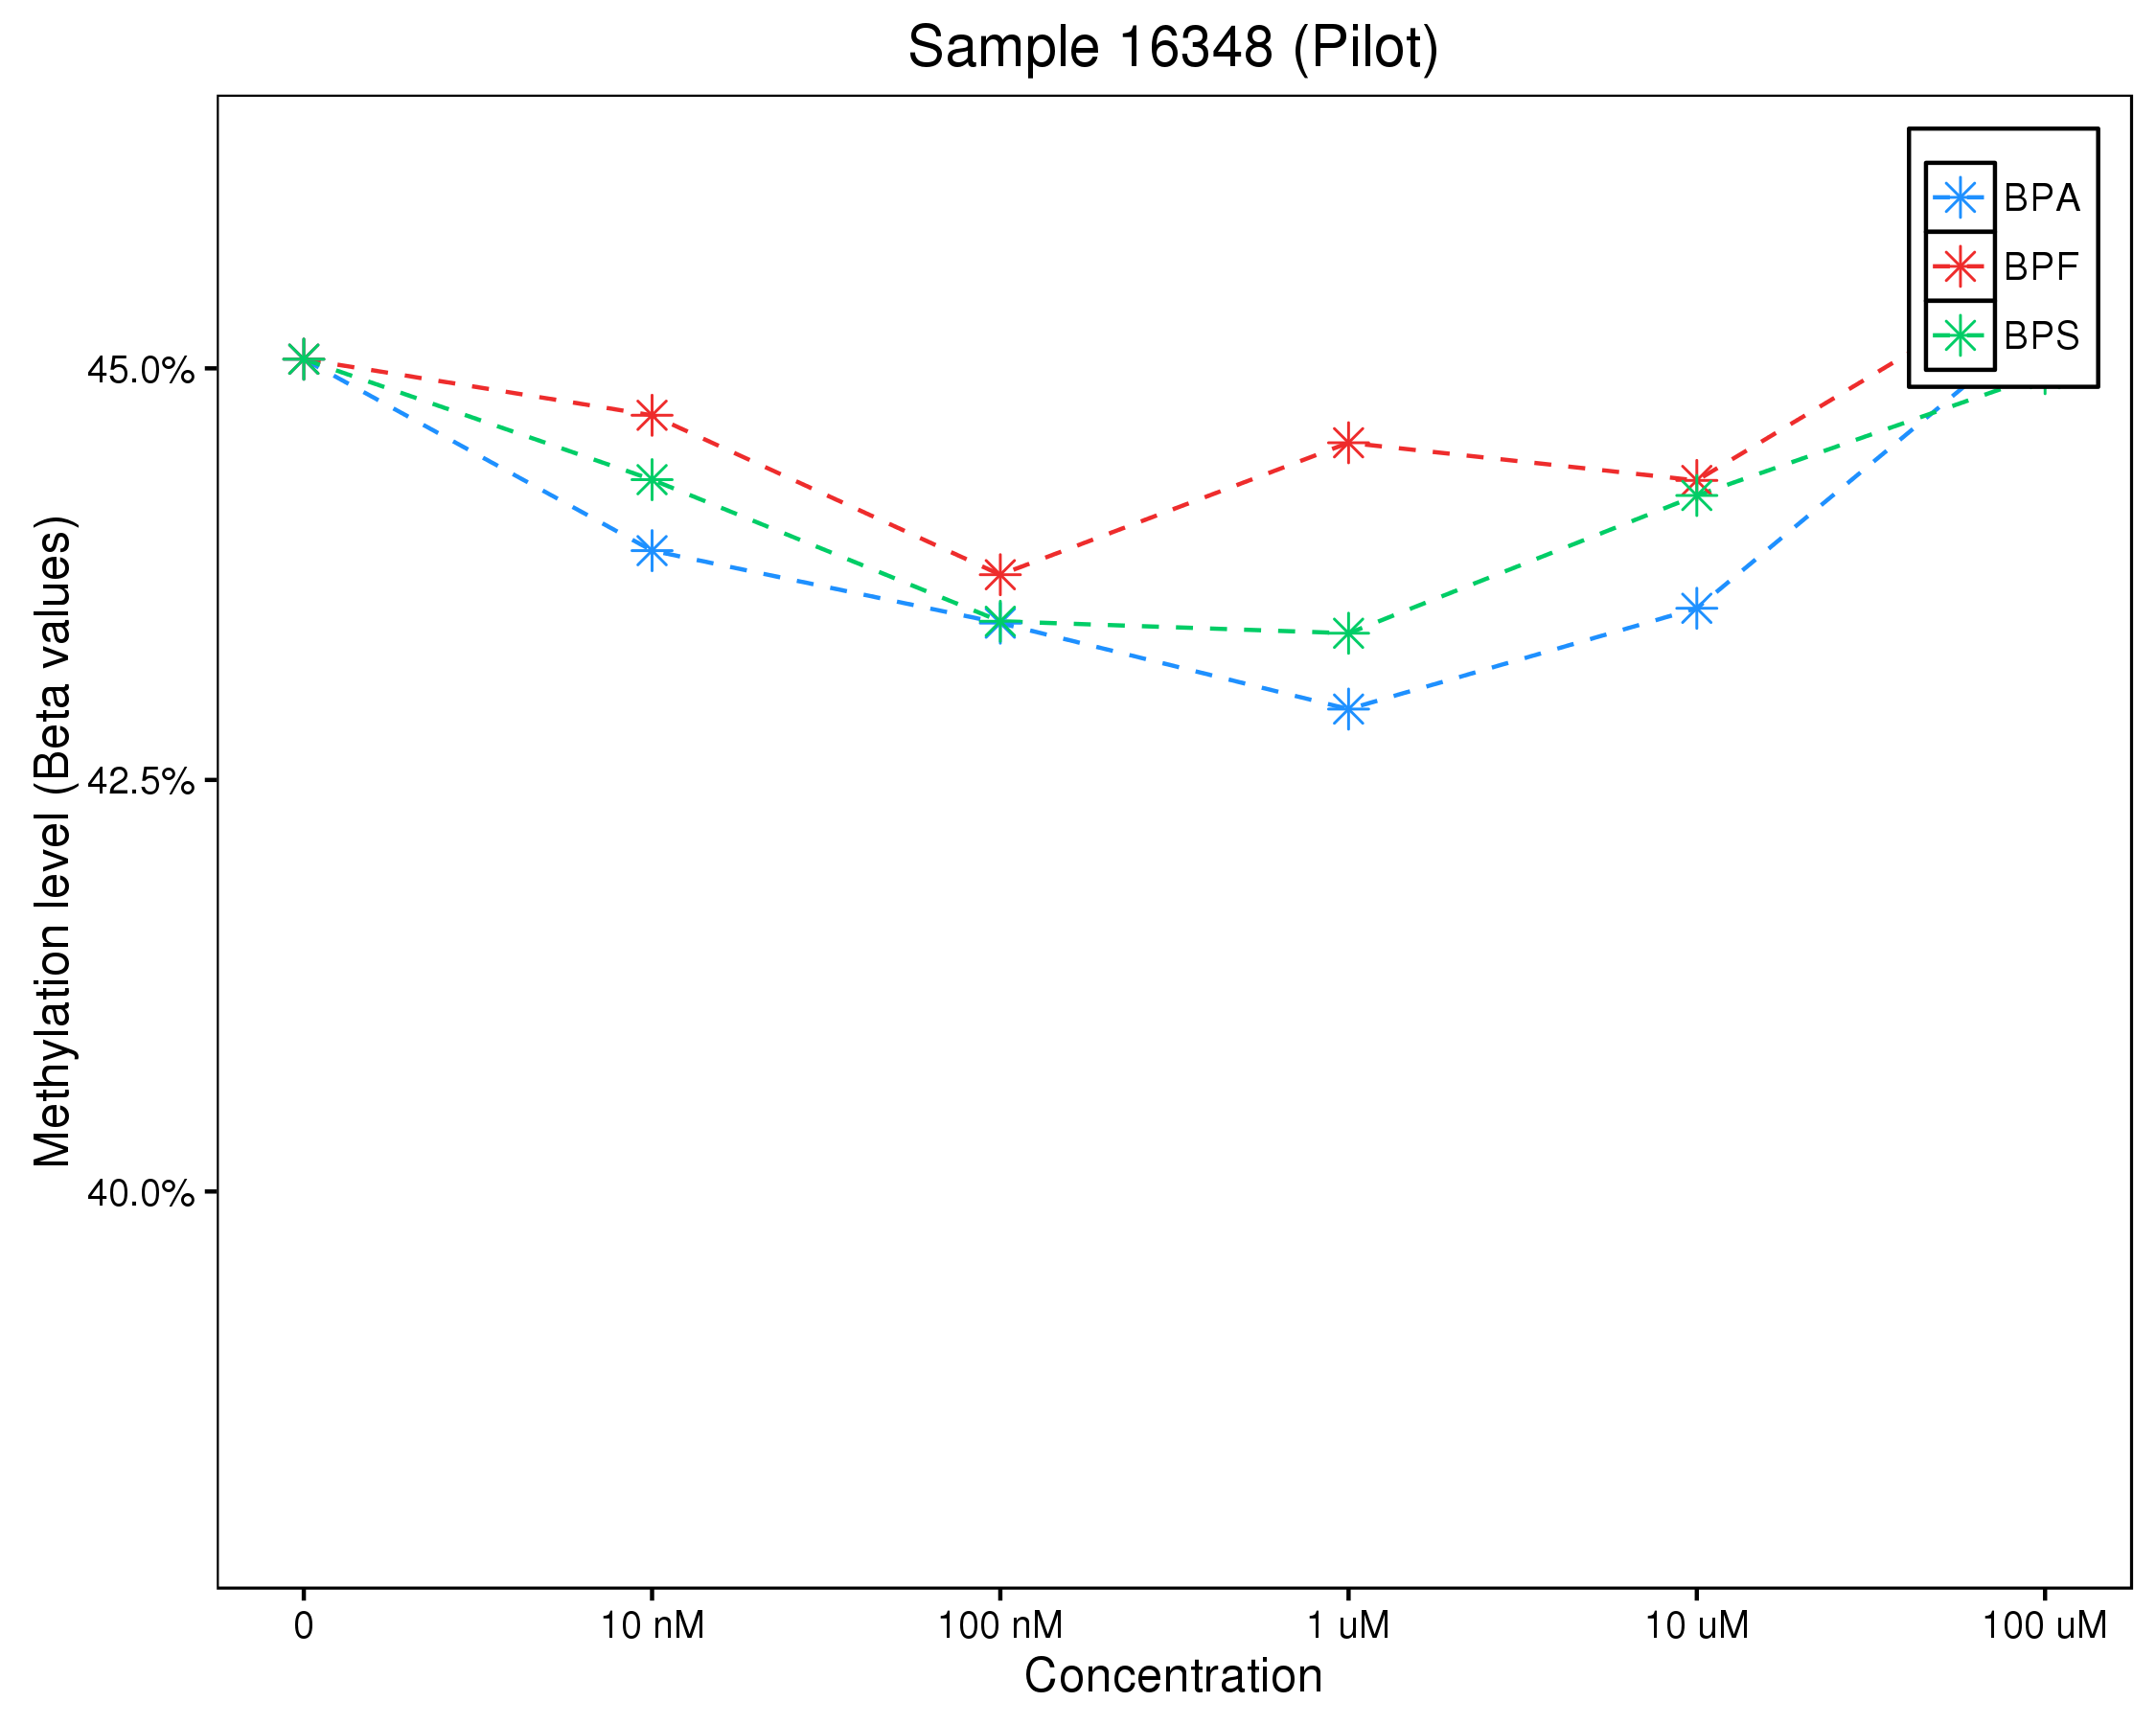
\includegraphics[width=3.75in,height=3in]{FiguresTables/ScatterPlot_GlobMethSample_16348_PilotAll} 

}

\caption{Profil de methylation globale selon
différentes concentrations de bisphénols A, F et S.}\label{fig:ScatterPlotGlobMethSample}
\end{figure}

Dans une étude pilote portant sur les cellules d'un patient, la
méthylation globale d'environ 381~000 sites CpG (puce Illumina
HumanMethylation 450K) a été analysée en fonction de la concentration en
bisphénol (10 nM, 100 nM, 1 µM, 10 µM et 100 µM), introduite dans le
milieu de culture lors de la différenciation des adipocytes primaires.
Ces premiers résultats suggéraient un effet dose-réponse de la
méthylation, pouvant être modélisé par un polynôme de degré deux (Figure
\ref{fig:ScatterPlotGlobMethSample}), dont les effets les plus
importants ont été observés au niveau du gène PTPRN2 (Protein Tyrosine
Phosphatase, Receptor type N2) avec 91 sites CpG présentant un effet
d'ordre deux significatif du logarithme de la concentration de
bisphénol. Ces sites présentaient une hypométhylation pour des
concentrations non physiologiques (c.-à-d. supérieures à 10 nM), et un
retour proche du niveau de méthylation pour une forte concentration de
100 µM, suggérant ainsi que la méthylation des adipocytes pouvait être
sensible à l'ajout de bisphénols dans le milieu, notamment pour des
concentrations de 10 nM et de 10 µM, tel qu'observé sur la méthylation
globale.

Conjointement à l'étude du transcriptome des adipocytes, le méthylome de
ces mêmes cellules a été examiné. Cependant, la forte variabilité inter
et intra-patients n'a pas permis, en plus du faible nombre de patients
(\(n=3\) en duplicats) d'identifier des sites CpG différentiellement
méthylés partagés entre les différents bisphénols. De plus,
contrairement à l'analyse transcriptomique où le statut de
différenciation des adipocytes a pu être évalué (via l'utilisation de
gènes spécifiquement exprimés dans les adipocytes matures), le méthylome
des adipocytes comparés aux adipocytes primaires n'a pas permis
d'identifier de marques de méthylation spécifiques reflétant cet état de
différenciation. Les mRNA et les miRNA identifiés dans l'analyse
transcriptomique ont fait l'objet d'une étude de corrélation avec les
sites CpG annotés (Illumina) sur les gènes correspondants. Aucune
corrélation significative entre les sondes miRNA/mRNA et la méthylation
n'a pu être mise en évidence, vraisemblablement en raison d'un manque de
puissance. Le faible nombre d'échantillons combiné à la variabilité de
la méthylation observée dans ces échantillons a probablement altéré
notre capacité à détecter des sites CpG impactés de façon similaire par
les bisphénols, malgré des études ayant démontré un effet sur la
méthylation du BPA, comme la déméthylation globale de l'ADN au cours de
la différenciation d'adipocytes (lignée cellulaire 3T3-L1)
\citep{bastos_sales_effects_2013}.

\section{Article}\label{article-3}

Article disponible en ligne sur \textbf{\emph{PLoS ONE}}
(\url{http://doi.org/10.1371/journal.pone.0179583}) \clearpage

\chapter*{Conclusion}\label{conclusion-4}


\setcounter{section}{0}

Nous proposons dans cette thèse une contribution au domaine de la
statistique génétique appliquée à la pathologie du diabète de type 2.
Cette contribution se scinde en deux aspects. Le premier aspect est un
développement méthodologique visant à améliorer les connaissances
actuelles et exploiter au mieux les données disponibles. Le second
aspect se concentre sur le support méthodologique et l'application des
méthodes adaptées aux questionnements inhérents aux différents projets
de recherche sur les données ``omiques''.

\section{Développement
méthodologique}\label{developpement-methodologique}

Deux principaux développements ont été réalisés au cours de cette thèse
(Chapitres \ref{Article1} et \ref{Article2})~:

\begin{itemize}
\item
  Le premier est une nouvelle approche, dans le domaine de la génétique,
  permettant de modéliser conjointement l'évolution d'un trait
  longitudinal et la survenue d'un événement, tout en évaluant l'effet
  des SNPs simultanément sur ces deux traits. Contrairement aux
  approches dites ``classiques'' des GWAS qui ont étudié l'effet des
  SNPs, d'une part, sur la glycémie à jeun dans des groupes d'individus
  normoglycémiques, et d'autre part, l'association des SNPs dans des
  études cas/témoins, l'approche par modèle joint que nous proposons
  dans cette thèse permet d'identifier des SNPs associés à l'évolution
  de la glycémie sans qu'ils ne soient nécessairement associés au risque
  de développement d'un diabète. De plus, nous apportons une solution au
  problème computationnel de l'application de cette approche à l'échelle
  du génome (p.~ex. puce-à-ADN imputée, séquençage, etc.), au moyen
  d'une méthode approchée dite en ``deux étapes''. Nous avons montré que
  l'approche en ``deux étapes'' est aussi robuste et précise que
  l'approche par modèle joint tout en offrant un gain en terme de temps
  de calcul.
\item
  Le second développement réalisé porte sur l'amélioration et
  l'automatisation de la récupération et l'analyse des données provenant
  de la technologie NanoString et de culture cellulaire. Dans ce second
  développement, j'ai réalisé deux applications web Shiny, nommées
  \emph{NanoStringTissueCartography} et \emph{EndoC\_Beta}~:

  \begin{itemize}
  \item
    L'application \emph{NanoStringTissueCartography} permet, en premier
    lieu, à partir des données brutes générées via la technologie
    NanoString, d'effectuer et de visualiser les différentes étapes du
    contrôle-qualité, ainsi que les niveaux d'expressions de plusieurs
    gènes de ménage, et en second lieu, d'analyser et de visualiser les
    données importées dans l'application, tout en offrant un cadre
    interactif. Par exemple, il est possible de sélectionner un ou
    plusieurs gènes selon une fonction, mais également de sélectionner
    les tissus d'intérêts, pour lesquels l'analyse d'expression et
    l'étude enrichissement doivent être réalisées.
  \item
    L'application \emph{EndoC\_Beta} permet d'inclure des fichiers de
    résultats au format Excel (ici, des mesures d'absorbance réalisées
    sur un modèle de cellule \(\beta\)) dès le remplissage de ces
    fichiers par les personnes en charge des expérimentations.
    L'agrégation de ces résultats dans un format standardisé permet de
    mesurer et de prendre en compte plusieurs facteurs techniques tels
    que l'expérimentateur, le jour d'expérimentation et la qualité de
    l'étalonnage des appareils, et de ce fait permet de réduire les
    biais que ces facteurs peuvent entraîner dans l'analyse. En outre,
    cette application permet différents niveaux de contrôle-qualité. Par
    exemple, j'ai incorporé une étape de contrôle de la gamme étalon
    utilisée pour estimer la sécrétion d'insuline. Cette étape vise à
    vérifier que les mesures d'absorbances observées, pour chaque
    concentration de référence, restent homogènes d'une expérience à
    l'autre, puisque le matériel (spectromètre et produits de référence
    de la gamme) est théoriquement le même. De plus, une erreur
    d'estimation de la pente de la gamme étalon (relation linéaire entre
    la concentration et l'absorbance) impactera l'ensemble des mesures
    utilisant celle-ci. Cette application, en plus de prendre en compte
    les facteurs techniques dans l'analyse, fournit un critère objectif
    quant à la mesure de sécrétion d'insuline par les cellules
    \(\beta\). En effet, le regroupement de l'ensemble des
    expérimentations réalisées sur les cellules \(\beta\) a permis
    d'établir un seuil à partir du ratio de la quantité d'insuline
    sécrétée dans la condition cible et dans la condition témoin. Ce
    seuil fournit une indication relative au développement des cellules
    \(\beta\) et donc indirectement sur la qualité de la culture.
  \end{itemize}
\end{itemize}

\section{Support méthodologique}\label{support-methodologique}

La nature et la complexité des données ``omiques'' nécessitent de
pouvoir identifier et appliquer une grande variété de méthodes connues
et/ou nouvelles pour s'adapter au mieux à la problématique des projets
de recherche. Il existe de nombreux articles traitant des méthodes
d'analyses des données de génomique, de transcriptomique et de
méthylomique. Cependant, le domaine de la méthylomique reste quant à lui
en retard par rapport aux deux autres, principalement en raison de son
caractère récent et en développement.\\
Les Chapitres \ref{Article3} et \ref{Article4}, sont le résultat des
études méthodologiques sur les trois ``omiques'' discutées dans cette
thèse, d'une part, au niveau des méthodes de contrôle-qualité plus ou
moins spécifiques, et d'autre part, au niveau des méthodes d'analyse
statistique. Dans ces deux chapitres, les études décrites ont fait
l'objet d'une étude pilote, en particulier pour étudier la méthylation
de l'ADN. Ces études pilotes ont permis l'identification et le
développement d'un processus d'analyse allant de la lecture des données
à la génération des résultats d'analyse, sur lequel se sont appuyées les
études définitives et les demandes de financement subséquentes. En
effet, ces résultats ont permis d'établir le nombre d'échantillon
nécessaire et/ou d'évaluer la puissance de l'étude, et d'élaborer les
plans d'expériences les mieux adaptés afin de réduire les biais
techniques ou les facteurs de confusion.

\section{Multi-omiques \&
Perspectives}\label{multi-omiques-perspectives}

Les différents projets abordés dans les Chapitres \ref{Article1},
\ref{Article2}, \ref{Article3} et \ref{Article4} s'inscrivent dans une
démarche multi-omiques, notamment par l'intégration de la méthylomique,
de la transcriptomique, de la génomique et de la phénomique (phénotype).
Néanmoins, cette intégration est partielle dans le sens où l'analyse est
réalisée sous la forme de filtres successifs~: par exemple dans le
Chapitre \ref{Article3}, l'analyse s'est concentrée sur la méthylomique,
puis les autres ``omiques'' ont été incluses pour apporter une nouvelle
couche ``mécanistique'' et ainsi remonter à la pathophysiologie. Cette
approche d'intégration successive des ``omiques'' offrent un cadre de
mise en oeuvre simple et robuste, et permet de mettre en évidence un
aspect mécanistique plus proche des hypothèses biologiques et cliniques,
que ne le permet une analyse séparée des ``omiques''.

Avec le développement de la médecine de précision, qui vise à
caractériser, à plusieurs niveaux, un individu et prédire son avenir
médical, des méthodes d'intégrations de données se sont développées
conjointement aux méthodes relatives au ``Big Data'' (c.-à-d. ``machine
learning'', tels que les ``neural network'') permettant de traiter des
gros volumes de données \citep{huang_more_2017, lin_machine_2017}. La
cohorte D.E.S.I.R. fournit un cadre idéal d'application et de
développement des approches pour données longitudinales et des approches
d'intégration de données. En effet, dans cette cohorte interrogée lors
de quatre vagues de mesure conduites à intervalle régulier sur une
période 9 ans, des données de différentes natures sont disponibles
telles que plus de 200 variables phénotypiques, des données de
génomique, de métabolomique (deux temps de mesure) et prochainement des
données de méthylomique (deux temps de mesure). À cela s'ajoute la mise
en place de consortia permettant de regrouper plusieurs laboratoires et
cohortes (p.~ex. RHAPSODY portant sur l'évaluation du risque et de la
progression du diabète de type 2 et du pré-diabète), établissant un
cadre de plus en plus adapté aux différentes méthodes décrites et
développées dans cette thèse.

\chapter*{Liste des communications
scientifiques}\label{liste-des-communications-scientifiques}


\setcounter{section}{0}

\section{Communications en lien avec la
thèse}\label{communications-en-lien-avec-la-these}

\subsection{Conférences}\label{conferences}

\begin{itemize}
\item Rocheleau, G., \underline{\textbf{Canouil, M.}}, Yengo, L., Froguel, P. (2015). Application of Joint Models in Genetic Association Studies. \textit{International Genetic Epidemiology Society - IGES}, Baltimore, United-States.

\item \underline{\textbf{Canouil, M.}}, Rocheleau, G., Yengo, L., Froguel, P. (2016). Longitudinal Genetic Modelling: Revisiting Associations of SNPs Associated with Blood Fasting Glucose in Normoglycemic Individuals. \textit{Statistical Methods for Post Genomic Data - SMPGD}, Lille, France.

\item \underline{\textbf{Canouil, M.}}, Froguel, P., Rocheleau, G. (2016). Single Nucleotide Polymorphisms Associated with Fasting Blood Glucose Trajectory and Type 2 Diabetes Incidence: A Joint Modelling Approach. \textit{International Genetic Epidemiology Society - IGES}, Toronto, Canada.

\item \underline{\textbf{Canouil, M.}}, Froguel, P., Rocheleau, G. (2016). Single Nucleotide Polymorphisms Associated with Fasting Blood Glucose Trajectory and Type 2 Diabetes Incidence: A Joint Modelling Approach. \textit{4th Symposium European Genomic Institute for Diabetes (E.g.i.d)}, Lille, France.

\item \underline{\textbf{Canouil, M.}}, Froguel, P., Rocheleau, G. (2017). Variants Génétiques Associés à la Trajectoire de la Glycémie à Jeun et à l’Incidence du Diabète de Type 2: Une Approche par Modèle Joint. \textit{Annual Congress of Société Francophone du Diabète (SFD)}, Lille, France. 
\end{itemize}

\clearpage

\subsection{Articles publiés dans des revues internationales à comité de
lecture}\label{articles-publies-dans-des-revues-internationales-a-comite-de-lecture}

\begin{itemize}
\item Ndiaye, F. K., Ortalli, A., \underline{\textbf{Canouil, M.}} \textit{et al.} (2017). Expression and functional assessment of candidate type 2 diabetes susceptibility genes identify four new genes contributing to human insulin secretion. \textit{Molecular Metabolism}.

\item Verbanck, M., \underline{\textbf{Canouil, M.}} \textit{et al.} (2017). Low-dose exposure to bisphenols A, F and S of human primary adipocyte impacts coding and non-coding RNA profiles. \textit{PLOS ONE}, 12(6), e0179583.
\end{itemize}

\section{Autres communications dans le domaine de la
génétique}\label{autres-communications-dans-le-domaine-de-la-genetique}

\begin{itemize}
\item Yengo, L., Jacques, J., Biernacki, C. and \underline{\textbf{Canouil, M.}} (2016). Variable Clustering in High-Dimensional Linear Regression: The R Package clere. \textit{The R Journal}, 8(1), 92–106.

\item Baumeier, C., Saussenthaler, S., Kammel, A., Jähnert, M., Schlüter, L., Hesse, D., \underline{\textbf{Canouil, M.}} \textit{et al.} (2017). Hepatic DPP4 DNA Methylation Associates With Fatty Liver. \textit{Diabetes}, 66(1), 25–35.

\item Carrat, G. R., Hu, M., Nguyen-Tu, M.-S., Chabosseau, P., Gaulton, K. J., van de Bunt, M., Siddiq, A., Falchi, M., Thurner, M., \underline{\textbf{Canouil, M.}} \textit{et al.} (2017). Decreased STARD10 Expression Is Associated with Defective Insulin Secretion in Humans and Mice. \textit{The American Journal of Human Genetics}, 100(2), 238–256.

\item Bonnefond, A., Yengo, L., Dechaume, A., \underline{\textbf{Canouil, M.}} \textit{et al.} (2017). Relationship between salivary/pancreatic amylase and body mass index: a systems biology approach. \textit{BMC Medicine}, 15(1).
\end{itemize}

\clearpage

\bibliography{bib/MyArticles,bib/Mickael_ThesisClean,bib/Rpackages}

\backmatter
\printindex

\end{document}
